%!TeX program = xelatex
\documentclass[a4paper, 12pt, twoside]{book}
\usepackage[top=2.5cm, bottom=3cm, left=2.25cm, right=1.75cm]{geometry}

%%% Fonts because I'm a nerd
\usepackage{setspace}
\usepackage{amsmath}
\def\myfont{1} % 0=MinionPro, 1=Times, 2=Libertine
\usepackage[MnSymbol]{mathspec}
\if\myfont0   % Minion Pro
    \setstretch{1.025}
    \setlength{\parskip}{5pt}
    \setlength{\parindent}{15pt}
    \setmainfont[
        Path = /Users/keruzore/Documents/fonts/,
        BoldFont={Minion Pro Bold.otf},
        ItalicFont={Minion Pro Italic.ttf},
        BoldItalicFont={Minion Pro Bold Italic.ttf},
        Scale=MatchLowercase
    ]{Minion Pro Regular.otf}
    \setmathsfont(Digits,Latin,Greek)[Numbers={Lining,Proportional}]{Minion Pro}
    \setmathrm[]{Minion Pro}
\else
    \setstretch{1.02}
    \setlength{\parskip}{10pt}
    \setlength{\parindent}{15pt}
    \if\myfont1   % Times/STIX/Termes
        \setmainfont{TeX Gyre Termes}
        \setmathsfont(Digits,Latin)[Scale=MatchLowercase]{TeX Gyre Termes}
        \setmathsfont(Greek)[Scale=MatchLowercase]{STIXGeneral}
        \setmathrm[]{STIXGeneral}
        \setmathcal[Scale=MatchUppercase]{TeX Gyre Chorus}
    \else\if\myfont2 % Linux Libertine
        \setmainfont{Linux Libertine O}
        \setmathsfont(Digits,Latin,Greek)[Scale=MatchLowercase]{Linux Libertine O}
        \setmathrm[]{Linux Libertine O}
    \fi
\fi
% Make digits be in correct font in URLs (this SUCKS)
\makeatletter
    \DeclareMathSymbol{0}{\mathalpha}{\eu@DigitsArabic@symfont}{`0}
    \DeclareMathSymbol{1}{\mathalpha}{\eu@DigitsArabic@symfont}{`1}
    \DeclareMathSymbol{2}{\mathalpha}{\eu@DigitsArabic@symfont}{`2}
    \DeclareMathSymbol{3}{\mathalpha}{\eu@DigitsArabic@symfont}{`3}
    \DeclareMathSymbol{4}{\mathalpha}{\eu@DigitsArabic@symfont}{`4}
    \DeclareMathSymbol{5}{\mathalpha}{\eu@DigitsArabic@symfont}{`5}
    \DeclareMathSymbol{6}{\mathalpha}{\eu@DigitsArabic@symfont}{`6}
    \DeclareMathSymbol{7}{\mathalpha}{\eu@DigitsArabic@symfont}{`7}
    \DeclareMathSymbol{8}{\mathalpha}{\eu@DigitsArabic@symfont}{`8}
    \DeclareMathSymbol{9}{\mathalpha}{\eu@DigitsArabic@symfont}{`9}
\makeatother

%%% Language options
\usepackage{polyglossia}
\setmainlanguage{french}
\usepackage{csquotes}

%%% Fix apostrophe kerning in MinionPro
\if\myfont0
    \makeatletter
    \edef\qu@te{\string'} % save a copy of the ordinary apostrophe
    \catcode`'=\active    % make ' active
    \begingroup
    \obeylines\obeyspaces%
    \gdef\@resetactivechars{%
    \def^^M{\@activechar@info{EOL}\space}%
    \def {\@activechar@info{space}\space}%
    }%
    \endgroup
    \providecommand\texorpdfstring[2]{#1}
    \protected\def'{\texorpdfstring{\texqu@te}{\string'}}
    \@ifpackagewith{inputenc}{utf8}
      {\DeclareUnicodeCharacter{2019}{\texqu@te}}{}
    \def\texqu@te{\relax
      \ifmmode
        \expandafter^\expandafter\bgroup\expandafter\prim@s
      \else
        \expandafter\futurelet\expandafter\@let@token\expandafter\qu@t@
      \fi}
    \def\qu@t@{%
      \ifx'\@let@token
        \qu@te\qu@te\expandafter\@gobble
      \else
        {\kern0em}\qu@te{\kern0em}\penalty\@M\hskip\expandafter\z@skip
      \fi}
    \scantokens\expandafter{%
      \expandafter\def\expandafter\pr@m@s\expandafter{\pr@m@s}}
    \makeatother
\fi

%%% Colors because I'm a nerd
\usepackage[dvipsnames]{xcolor}
\usepackage[colorlinks, allcolors=Maroon]{hyperref}

%%% Good looking sections&chapters
\usepackage{titlesec}
\titleformat{\chapter}[display]
  {\normalsize\huge\color{black}}%
  {\flushright\huge\color{Maroon}%
   \MakeUppercase{\chaptertitlename}\hspace{1ex}%
   {\bfseries\fontsize{40}{40}\selectfont\thechapter}}%
  {10 pt}%
  {\flushright\bfseries\Huge}%
\titlespacing\section{0pt}{12pt plus 2pt minus 2pt}{5pt plus 2pt minus 2pt}
\titlespacing\subsection{0pt}{12pt plus 2pt minus 2pt}{5pt plus 2pt minus 2pt}
\titlespacing\subsubsection{0pt}{12pt plus 2pt minus 2pt}{5pt plus 2pt minus 2pt}

%%% Mini table of contents at the beginning of chapters
\usepackage{minitoc}
\setcounter{minitocdepth}{2}
\setcounter{tocdepth}{2}

% Remove bottom page number from ALL pages
\makeatletter
  \let\ps@plain\ps@empty
\makeatother

%%% Headers and footers
\usepackage{fancyhdr}
\pagestyle{fancy}
\fancyhf{}
\fancyhead[RE]{\rightmark}
\fancyhead[LO]{\leftmark}
\fancyhead[RO,LE]{\thepage}
\fancyfoot[C]{}

%%% Misc
\usepackage{graphicx}               % figures
\usepackage[font=footnotesize]{caption}
\usepackage[rightcaption]{sidecap}  % caption on side
\sidecaptionvpos{figure}{c}
\usepackage{afterpage}              % Force next page on figures
%\usepackage{parskip}                % Set length between paragraphs
\usepackage{booktabs}               % better table rules
\usepackage{tabularx}               % control widths
\usepackage{multirow}               % multi-row cells in tables
\usepackage{enumitem}               % better lists
\usepackage{lipsum}                 % Latin placeholder text
\usepackage{hyperref}               % hyperlinks
\usepackage{afterpage}
\usepackage{cleveref}
\usepackage[toc,page]{appendix}     % Appendices
\usepackage{stackengine}            % Stack figures
\usepackage{pdfpages}               % Add ADUM cover
\usepackage{scrextend}              % To make function forcing even last page

%%% Itemize bullet
\renewcommand{\labelitemi}{--}

%%% Clear bib
\usepackage[%
    backend=biber,
    style=numeric,
    citestyle=numeric-comp,
    sorting=none,
    giveninits=true,
    mincitenames=1, % only cite {min} authors et al. when
    maxcitenames=2, % there are more than {max} total
    backref=true,
]{biblatex}
\renewbibmacro{in:}{,}
\DeclareFieldFormat{postnote}{#1}
% clickable links without full URL
\DefineBibliographyStrings{french}{url = {link}}
\DeclareFieldFormat{url}{%
  \ifhyperref
    {\href{#1}{Lien}}
    {\url{#1}}
}
\DefineBibliographyStrings{french}{phdthesis = {Thèse de doctorat}}
%
\addbibresource{phd.bib}
\AtEveryBibitem{%
    \clearfield{urlyear}%
    \clearlist{language}%
    \clearfield{month}%
    \clearfield{day}%
    \clearfield{issn}%
    \clearfield{doi}%
    \clearfield{series}%
    \clearfield{eid}%
    \clearlist{publisher}%
    \clearfield{note}
}

% Italicize et al.
\renewbibmacro*{name:andothers}{% Based on name:andothers from biblatex.def
  \ifboolexpr{
    test {\ifnumequal{\value{listcount}}{\value{liststop}}}
    and
    test \ifmorenames
  }
    {\ifnumgreater{\value{liststop}}{1}
       {\finalandcomma}
       {}%
     \andothersdelim\bibstring[\emph]{andothers}}
    {}
}

% Remove weird random smallcaps coming from french (why?)
\addto\captionsfrench{\def\figurename{Figure}}
\addto\captionsfrench{\def\tablename{Table}}
\DefineBibliographyExtras{french}{\restorecommand\mkbibnamefamily} % author names in bib

%%% Ensure last page has even number
\newcommand{\OpenNewPageIfNeeded}{%
  \ifthispageodd{%
    \newpage
    \null
  }{%
  }%
}

%%% New commands
\renewcommand{\d}{\mathrm{d}}
\newcommand{\N}{\mathcal{N}\,}
\newcommand{\da}{\mathcal{D}_\textsc{a}}
\newcommand{\pdv}[2]{\frac{\partial #1}{\partial #2}}
\newcommand{\pdvsq}[2]{\frac{\partial^2 #1}{\partial #2^2}}
\newcommand{\unit}[1]{\rm #1}
\newcommand{\xt}{\vec{x}, t}
\newcommand{\ym}{{Y|M}}
\newcommand{\yz}{{Y|Z}}
\newcommand{\yzb}{{Y\,|\,Z}}
\newcommand{\e}{{\rm e}}
\newcommand{\eg}{voir par exemple}
\newcommand{\act}{ACT-CL~J0215.4+0030} % ultimate laziness
\newcommand{\prior}{\textit{a priori}} % ultimate laziness
\newcommand{\addref}{{\color{Red}\bfseries [ADD REF]}}
\newcommand{\todo}[1]{{\color{Red}\bfseries [TODO: #1]}}
\newcommand{\myciteauthor}[1]{\citeauthor{#1} \cite{#1}}
\newcommand{\myfullcite}[1]{%
    \citeauthor{#1}, %
    \citefield{#1}{journaltitle} \citefield{#1}{volume}, \citefield{#1}{pages}, %
    \citeyear{#1} \cite{#1}%
}
\newcommand{\mypageref}[1]{\ref{#1} (page \pageref{#1})}


%%% Begin
\title{Cosmologie avec des amas de galaxies à partir d'observations de l'effet Sunyaev-Zeldovich avec la caméra NIKA2}
\author{Florian \textsc{K\'eruzor\'e}}
\date{}

\begin{document}

\begin{titlepage}
    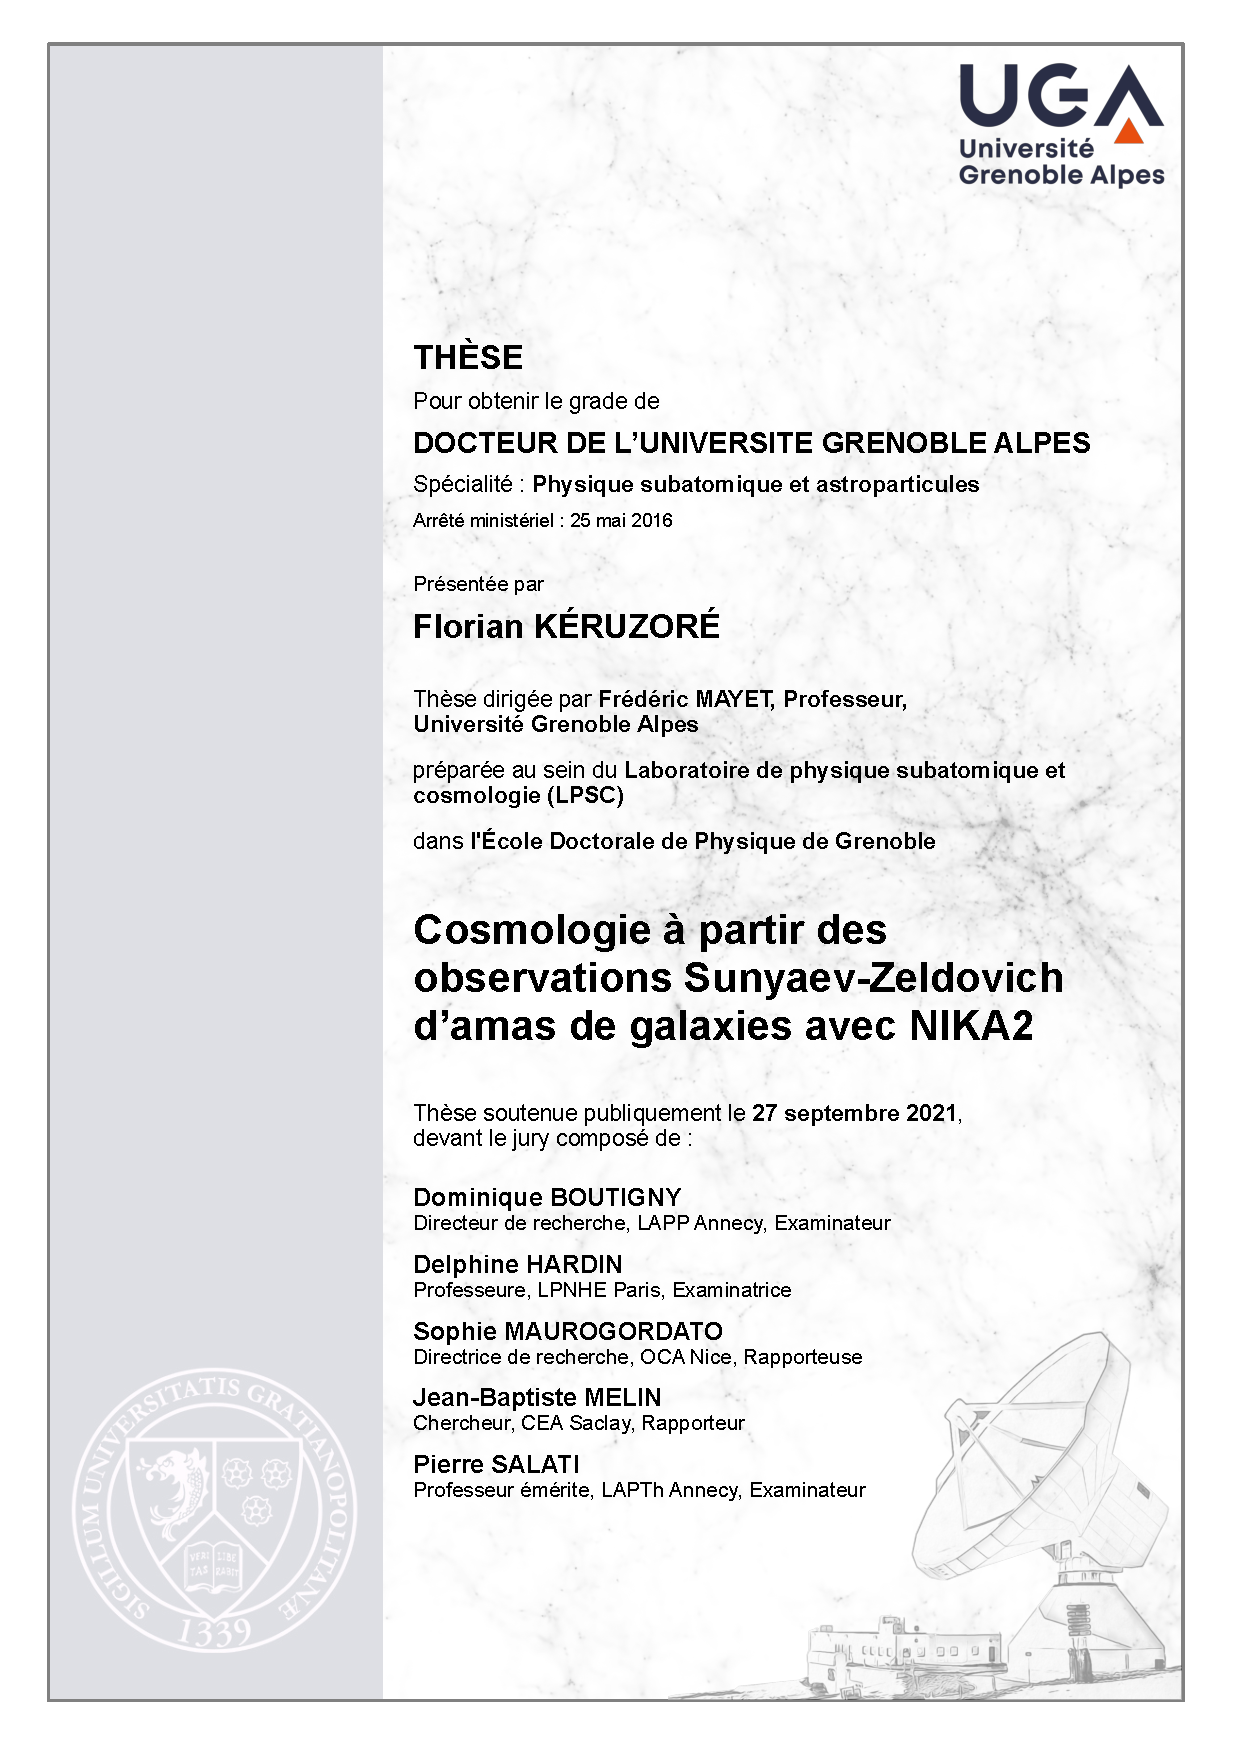
\includepdf[pages={1}]{couverture.pdf}
\end{titlepage}

\phantom{ }
\vfill
{\footnotesize \noindent
    Image de couverture: toile cosmique dans la simulation Millenium,
    crédit: Springel \textit{et al.} (2005) \cite{springel_simulations_2005}, \\
    \url{https://wwwmpa.mpa-garching.mpg.de/galform/virgo/millennium/} \\
    Télescope de 30 mètres de l'IRAM
}

\setlength{\parskip}{2.5pt}
%\newpage
\dominitoc[n]
\tableofcontents
\adjustmtc
\setlength{\parskip}{5pt}

% ==================================================================================== %

\chapter*{Introduction}
\label{chap:intro}
\addcontentsline{toc}{chapter}{\nameref{chap:intro}}
\markboth{}{\uppercase{Introduction}}
Les vingt dernières années ont été l'époque de l'essor de la cosmologie observationnelle.
Le développement de grandes expériences permettant de réaliser des relevés profonds du ciel avec une grande précision a permis d'accroître notre connaissance des propriétés de l'Univers.
En particulier, les paramètres cosmologiques ont pu être contraints avec une grande précision en ajustant les paramètres libres du modèle standard de la cosmologie à partir de ces données.
L'utilisation de plusieurs sondes pour mesurer ces paramètres cosmologiques a permis de tirer profit des différentes sensibilités des observables aux propriétés de l'Univers.
Si la plupart de ces mesures concordent, certains désaccords subsistent, pouvant être le signe de physique encore inconnue, ou bien d'effets systématiques non-maîtrisés.
Avec l'augmentation de la quantité des données disponibles et la diminution des incertitudes statistiques résultante, ces effets deviendront de plus en plus dominants.
La cosmologie observationnelle devient donc une science de grande précision, ce qui crée un besoin d'études rigoureuses des systématiques associées aux analyses cosmologiques.

Dans ce contexte, les amas de galaxies sont des objets d'un grand intérêt.
Leur abondance en masse et en redshift est étroitement liée à la distribution de masse dans l'Univers.
Cette dernière étant intimement liée aux paramètres cosmologiques, le comptage d'amas dans l'Univers par intervalles de masse et redshift peut être utilisé comme une sonde cosmologique.
De grands catalogues d'amas ont pu être compilés au cours des dernières années, qui exploitent les observables des amas dans différentes longueurs d'onde pour les détecter dans de grands relevés du ciel.
Parmi les observables utilisées, l'effet Sunyaev-Zeldovich (SZ) permet de détecter les amas dans le domaine millimétrique, grâce à leur empreinte sur le fond diffus cosmologique.
Les catalogues les plus récents construits grâce à l'effet SZ ont été obtenus à partir des télescopes ACT (Atacama Cosmology Telescope, \cite{hilton_atacama_2021}), SPT (South Pole Telescope, \cite{bleem_galaxy_2015,bleem_sptpol_2020}) et du satellite \textit{Planck} \cite{planck_collaboration_planck_2016-3}, et comportent plusieurs milliers d'amas.
Dans le futur, le Simons Observatory \cite{ade_simons_2019} et CMB-S4 \cite{abazajian_cmb-s4_2016} augmenteront ce nombre par un à deux ordres de grandeur, et seront accompagnés par les relevés du Vera Rubin Observatory \cite{lsst_dark_energy_science_collaboration_large_2012} et d'\textit{Euclid} \cite{sartoris_next_2016} en optique et infrarouge, et d'eROSITA \cite{pillepich_forecasts_2018} en X.

Ainsi, à l'instar de la cosmologie observationnelle dans laquelle elle s'inscrit, la cosmologie avec des amas entre dans une ère de précision, avec un grand nombre de catalogues comportant chacun de grands nombres d'amas.
Le contrôle des systématiques s’avère être d’une importance cruciale, afin de pouvoir tirer pleinement profit de ces catalogues d'amas comme sondes cosmologiques.
Cette maîtrise est actuellement limitée par une faible connaissance des propriétés physiques des amas de galaxies, en particulier des amas distants.
En effet, une caractérisation précise de la physique des amas est nécessaire à leur exploitation cosmologique.
Dans le cadre des relevés de l'effet SZ mentionnés précédemment, cette connaissance est limitée aux objets proches du fait de la faible résolution angulaire des instruments.
Il est donc nécessaire de compléter ces relevés avec des suivis d'amas distants, en utilisant des instruments à haute résolution.
Parmi ces études, le grand programme SZ de NIKA2 réalise un suivi d'amas distants détectés par \textit{Planck} et ACT avec la caméra millimétrique à grande résolution angulaire NIKA2, installée au télescope de 30 mètres de l'IRAM \cite{perotto_calibration_2020}.
L'objectif de ce suivi est d'exploiter les observations SZ résolues pour mesurer deux outils nécessaires à la cosmologie à partir de relevés SZ: le profil de pression moyen des amas de galaxies, et la relation d'échelle masse-observable.
Ces outils sont actuellement étalonnés sur des amas proches, en utilisant des observations SZ à basse résolution ou X.

Le travail développé au cours de cette thèse s'inscrit dans le cadre du grand programme SZ de NIKA2, et de l'étude des effets systématiques en cosmologie avec des amas détectés par effet SZ.
Ce manuscrit présente le travail effectué, de l'analyse des données NIKA2 aux prédictions des contraintes pouvant être mises sur la relation d'échelle masse-observable grâce au grand programme SZ, en passant par la mesure des propriétés thermodynamiques des amas de galaxies en tenant compte des systématiques caractéristiques des observations millimétriques.
Il se découpe en sept chapitres.
\begin{itemize}[leftmargin=*]
\setlength\itemsep{5pt}
\item
    Le chapitre \ref{chap:cosmo1} présente le contexte du modèle standard de la cosmologie, en décrivant le lien entre le contenu de l'Univers et ses propriétés, et la formation des grandes structures.
    Il permet d'introduire les éléments importants des analyses cosmologiques basées sur des amas de galaxies.
\item
    Le chapitre \ref{chap:amas} est consacré aux amas de galaxies et à leur utilisation en cosmologie.
    La définition des amas de galaxies, leur composition et leurs caractéristiques sont présentées, de même que les différentes possibilités pour les observer.
   Nous décrivons le lien entre la distribution d'amas en masse et en redshift et les paramètres cosmologiques, et les analyses par comptage d'amas permettant de contraindre ces derniers à partir de catalogues d'amas.
   Nous présentons quelques-uns des résultats les plus récents de telles études, et les expériences à venir.
\item
    Le chapitre \ref{chap:nika2} présente la caméra NIKA2 au télescope de 30 mètres de l'IRAM, ainsi que son grand programme SZ.
    Nous décrivons les caractéristiques techniques du télescope et de NIKA2, notamment les détecteurs à inductance cinétiques de cette caméra.
    Les performances de l'instrument sont également présentées, de même que les observations au télescope, que j'ai pu réaliser en participant à cinq semaines d'observation au télescope au cours des 18 premiers mois de ma thèse, puis trois semaines d'observations à distance.
    Nous présentons les caractéristiques du grand programme SZ de NIKA2, son échantillon d'amas, et ses objectifs scientifiques.
\item
    Le chapitre \ref{chap:decorr} décrit la procédure utilisée pour construire des cartes de l'effet SZ à partir des données brutes de NIKA2.
    Nous présentons tout d'abord la procédure employée pour séparer le signal astrophysique d'intérêt du bruit dans les données.
    Cette procédure, nommée décorrélation, nécessite un traitement complexe du bruit dans les données, car celui-ci est plusieurs ordres de grandeur supérieur au signal d'intérêt.
    Nous présentons l'évaluation de la performance de la décorrélation et des systématiques qu'elle induit, qui sont prises en compte au cours de l'analyse des cartes SZ résultantes.
    Nous décrivons également la procédure mise en place pour estimer la contamination des cartes SZ par des sources ponctuelles.
\item
    Le chapitre \ref{chap:panco} présente le logiciel \texttt{PANCO2}, que j'ai développé au cours de ma thèse.
    L'objectif de ce programme est de contraindre les propriétés thermodynamiques des amas de galaxies à partir d'observations SZ par analyse Monte Carlo à chaînes de Markov.
    Le développement d'un nouveau logiciel pour de telles analyses était nécessaire pour des raisons de performance: les outils existants ne permettaient pas de réaliser l'analyse d'un échantillon d'amas en un temps raisonnablement court.
    Son fonctionnement permet de tenir compte des effets systématiques caractéristiques des observations SZ, comme la corrélation du bruit résiduel, le filtrage du signal, et la contamination par des sources ponctuelles.
    Nous décrivons le fonctionnement du logiciel et les propriétés physiques qu'il permet de sonder, puis présentons sa validation sur des données simulées.
    \texttt{PANCO2} est le \textit{pipeline} officiel pour l'analyse des données du grand programme SZ de NIKA2, et une généralisation est en cours pour qu'il puisse être utilisé pour d'autres instruments.
    Ce logiciel sera alors rendu public pour la communauté scientifique.
\item
    Le chapitre \ref{chap:actj0215} est dédié à l'analyse des propriétés thermodynamiques de l'un des amas les plus complexes du grand programme SZ, \act.
    Il représente l'un des amas de plus faible masse et de plus haut redshift de l'échantillon, et le premier amas du programme pour lequel les observations NIKA2 sont de qualité standard.
    De plus, le signal SZ de l'amas est fortement contaminé par des sources ponctuelles, dont le flux masque le signal de l'amas.
    Nous présentons l'extraction des propriétés thermodynamiques de l'amas en considérant les sources ponctuelles comme des paramètres de nuisance de l'analyse, dont le flux est connu \prior\ grâce à des observations du satellite \textit{Herschel}.
    Nous combinons les observations SZ avec NIKA2 avec des données X obtenues par le satellite \textit{XMM-Newton}, ce qui permet une caractérisation complète des propriétés de l'amas.
    %Bien que l'analyse soit complexe, nous réussissons à obtenir des contraintes fortes sur les propriétés de l'amas, ce qui témoigne du pouvoir de contrainte des observations avec NIKA2.
\item
    Enfin, le chapitre \ref{chap:scaling} présente la relation d'échelle liant la masse des amas à leur observable dans les relevés SZ.
    Nous présentons une approche probabiliste basée sur un modèle bayésien hiérarchique.
    Cette approche permet de tenir compte d'un grand nombre d'effets systématiques caractéristiques des relations masse-observable, comme la dispersion ou le biais des estimateurs de masse, la dispersion intrinsèque autour de la relation, et les effets de sélection.
    Nous appliquons cette modélisation à des simulations réalistes d'échantillons d'amas similaires au grand programme SZ de NIKA2, ce qui permet d'identifier les biais et systématiques et de prévoir les incertitudes attendues sur les paramètres de la relation à l'issue du grand programme SZ.
    Nous utilisons également cet outil pour évaluer l'intérêt d'extensions du grand programme SZ.
\end{itemize}


% ------------------------------------------- %
\chapter{Évolution de l'Univers et des grandes structures}
\label{chap:cosmo1}
\minitoc
%Cette thèse parle de la cosmologie avec des amas de galaxies.
%Pour comprendre, il faut donc savoir ce que c'est la cosmologie.
%Dans ce chapitre, on fait ça.

Le modèle standard de la cosmologie offre un formalisme décrivant l'évolution de l'Univers, du \textit{Big Bang} à aujourd'hui.
Ses succès observationnels sont nombreux, de l'expansion de l'Univers à l'existence du fond diffus cosmologique, en passant par la nucléosynthèse primordiale; aujourd'hui, il n'existe pas d'observations le mettant en échec.
Dans ce cadre, les propriétés de l'Univers sont décrites par un nombre restreint de quantités, nommées paramètres cosmologiques, dont la mesure est aujourd'hui l'enjeu de la cosmologie observationnelle.
Cette thèse s'inscrit dans ce cadre, et propose en particulier de contribuer à l'étude des mesures des paramètres cosmologiques en utilisant les amas de galaxies comme sondes cosmologiques.

Ce chapitre décrit les éléments nécessaires à la compréhension des analyses cosmologiques basées sur des amas de galaxies.
Nous commençons par présenter le modèle $\Lambda {\rm CDM}$, ou modèle standard de la cosmologie, décrivant le lien entre le contenu de l'Univers et sa dynamique.
Nous décrivons ensuite la formation des grandes structures, de leur origine à l'issue de l'inflation à leur développement récent par croissance des instabilités.

% ===================================================================================== %
\section{Le modèle standard de la cosmologie}

% ------------------------------------------------------------------------------------- %
\subsection{Les équations de Friedmann}\label{sec:friedmann}

La cosmologie moderne décrit l'Univers comme un objet dynamique obéissant aux lois de la relativité générale.
Ce cadre permet de lier la structure de l'espace-temps avec le contenu de l'Univers au travers des équations d'\myciteauthor{einstein_feldgleichungen_1915}:
\begin{equation}
    \label{eq:einst_field}
    G_{\mu\nu} + \Lambda g_{\mu\nu} = \frac{8\pi G}{c^4} T_{\mu\nu}.
\end{equation}
La partie gauche de l'équation encode la géométrie de l'espace-temps au travers du tenseur d'Einstein $G_{\mu\nu}$ et de la métrique $g_{\mu\nu}$, et la partie droite décrit la dynamique des composants de l'Univers par leur tenseur énergie-impulsion $T_{\mu\nu}$.
$G$ est la constante gravitationnelle Newtonienne, $c$ la vitesse de la lumière dans le vide, et $\Lambda$ la constante cosmologique, qui sera discutée en section \ref{sec:dark_energy}.
Dans l'hypothèse d'un Univers globalement homogène et isotrope, la solution dynamique la plus simple de l'équation (\ref{eq:einst_field}) est donnée par la métrique de Friedmann–Lemaître–Robertson–Walker (FLRW):
\begin{equation}
    \label{eq:flrw}
    \d s^2 = g_{\mu\nu} \d x^\mu \d x^\nu = c^2 \d t^2 - a^2(t) \left[ \frac{1}{1 - kr^2} \d r^2 + r^2 \d\theta^2 + r^2 \sin^2\theta \, \d\phi^2 \right],
\end{equation}
où $(t, r, \theta, \phi)$ sont les coordonnées sphériques à quatre dimensions. \\
Le paramètre de courbure $k$ caractérise la géométrie globale de l'Univers, qui peut être hyperbolique ($k=-1$), sphérique ($k=1$), ou plate ($k=0$, cas favorisé par les observations).
La fonction $a(t)$ est le facteur d'échelle de l'Univers, décrivant son expansion.
Son expression peut être écrite en considérant le contenu de l'Univers comme un fluide parfait comobile de densité d'énergie $\rho$ et de pression $p$, dont le tenseur énergie-impulsion s'écrit en fonction de la quadri-vitesse du fluide $u^\mu$
\begin{equation}
    \label{eq:tmunu}
    T^{\mu\nu} = (p/c^2 + \rho)u^\mu u^\nu - p g^{\mu\nu}.
\end{equation}
Alors, la combinaison des équations (\ref{eq:einst_field}), (\ref{eq:flrw}) et (\ref{eq:tmunu}) permet d'aboutir aux équations de Friedmann:
\begin{equation}
    \label{eq:fried1}
    H^2(t) \equiv \left(\frac{\dot{a}}{a}\right)^2 = \frac{8\pi G}{3} \rho + \frac{\Lambda c^2}{3} - \frac{kc^2}{a^2}
\end{equation}
\begin{equation}
    \label{eq:fried2}
    \frac{\ddot{a}}{a} = -\frac{4\pi G}{3} \left(\rho + \frac{3}{c^2} p\right) + \frac{\Lambda c^2}{3}
\end{equation}
où $\dot{a}$ dénote la dérivée temporelle de $a$, et $H(t)$ est le paramètre de Hubble, quantifiant le taux d'expansion de l'Univers.

Ces équations différentielles lient la dynamique de l'Univers à l'évolution de la densité d'énergie et de pression de son contenu.
Cette évolution dépend du paramètre d'équation d'état $w=p/\rho c^2$ du fluide: la combinaison des équations (\ref{eq:fried1}) et (\ref{eq:fried2}) donne l'équation de conservation de l'énergie pour un fluide parfait comobile,
\begin{equation}
    \dot{\rho} = -3(\rho + p/c^2) \times H(t),
\end{equation}
et donc l'évolution avec le facteur d'échelle de la densité d'énergie $\rho$:
\begin{equation}
    \label{eq:rho_w}
    \rho(a) \propto a^{-3(1+w)}
\end{equation}
Le contenu de l'Univers peut être séparé en plusieurs fluides parfaits comobiles, notés $j$, représentant les différents constituants de l'Univers, et possédant chacun un paramètre d'état $w_j$.
Ces constituants sont la matière, comprenant l'ensemble des baryons de l'Univers, ainsi que la matière sombre, et le rayonnement, composé des photons et autres espèces relativistes de l'Univers.
L'équation de Friedmann (\ref{eq:fried1}) peut s'écrire en fonction des densités $\rho_j$ des différents constituants $j$ de l'Univers:
\begin{equation}
    H^2(a) = \frac{8\pi G}{3 }\sum_j \rho_j(a) + \frac{\Lambda c^2}{3} - \frac{kc^2}{a^2}
\end{equation}
où $H_0$ est le taux d'expansion actuel de l'Univers. \\
Ainsi, en introduisant la densité critique $\rho_c$ comme:
\begin{equation}
    \label{eq:rho_crit}
    \rho_c(a) \equiv \frac{3 H^2(a)}{8 \pi G},
\end{equation}
on peut définir les abondances relatives de chaque composante comme $\Omega_j \equiv \rho_j / \rho_c$.
La constante cosmologique et la courbure peuvent donc être considérées comme des constituants supplémentaires de l'Univers, d'abondances relatives respectives $\Omega_\Lambda \equiv \Lambda c^2 / 3H^2$ et $\Omega_k \equiv -kc^2 / (aH)^2$.
La première équation de Friedmann (\ref{eq:fried1}) s'écrit finalement:
\begin{equation}
    \label{eq:fried_omega}
    H^2(a) = H_0^2 \sum_i \Omega_{i,0} \, a^{-3(1+w_i)},
\end{equation}
où les composantes $i$ comprennent les constituants précédemment notés $j$ (matière et rayonnement), ainsi que la courbure et la constante cosmologique.
Leurs abondances relatives actuelles sont notées $\Omega_{i,0}$.
Les différents constituants de l'Univers, leurs paramètres d'équation d'état, et leur abondances actuelles mesurées par l'analyse des anisotropies du fond diffus cosmologique (ou CMB pour \textit{Cosmic Microwave Background}) par le satellite \textit{Planck} \cite{planck_collaboration_planck_2020} sont résumés dans la table \ref{tab:cosmo_params}.

\begin{table}[t]
    \small
    \centering
    \begin{tabular}{c c c}
        \toprule
        Composante $i$ & $w_i$ & $\Omega_{i,0}$ \\
        \midrule
        Matière $m$                         & $0$     & $0.3111 \pm 0.0056$ \\
        Rayonnement $r$                     & $1/3$   & $\sim 10^{-5}$ \\
        Constante cosmologique $\Lambda$    & $-1$    & $0.6889 \pm 0.0056$ \\
        Courbure $k$                        & $-1/3$  & $0.0007 \pm 0.0019$ \\
        \bottomrule
    \end{tabular}
    \caption{%
        Paramètres d'état $w$ et abondances actuelles $\Omega_0$ des constituants de l'Univers issues de l'analyse des anisotropies du fond diffus cosmologique mesurées par \textit{Planck} \cite{planck_collaboration_planck_2020}.
    }
    \label{tab:cosmo_params}
\end{table}

% ------------------------------------------------------------------------------------- %
\subsection{Expansion de l'Univers, accélération et énergie sombre}
\label{sec:dark_energy}

Les équations de Friedmann permettent de lier l'évolution du facteur d'échelle de l'Univers aux densités d'énergie de ses différents constituants, et d'étudier cette évolution dans le temps.
D'après la combinaison de la première équation de Friedmann (\ref{eq:fried_omega}) et de l'équation (\ref{eq:rho_w}), il apparait que le facteur d'échelle d'un Univers de densité d'énergie dominée par un constituant d'équation d'état $w \geqslant -1$ ne peut qu'augmenter avec le temps.
Chacun des constituants de notre Univers vérifiant cette condition (comme montré en table \ref{tab:cosmo_params}), nous pouvons en déduire que celui-ci est en expansion.
Cette expansion se caractérise par une dilatation de l'espace-temps avec le temps, et une augmentation des distances séparant les différents objets présents dans l'Univers.
Il en découle que par le passé, l'Univers entier était contenu dans un volume bien plus faible qu'aujourd'hui, diminuant en remontant le temps jusqu'à atteindre une singularité de l'espace-temps: c'est le modèle du \textit{Big Bang}, élément majeur de notre compréhension de la cosmologie.

Historiquement, la constante cosmologique $\Lambda$ fût introduite par Einstein dans les équations du champ (\ref{eq:einst_field}) afin de pouvoir décrire un modèle d'Univers statique.
Cette hypothèse fût mise en échec par les confirmations observationnelles de l'expansion par \myciteauthor{lemaitre_univers_1927} et \myciteauthor{hubble_relation_1929}.
Ces études ont mis en évidence le décalage vers le rouge des spectres de galaxies l'expansion: un photon émis a un instant $t_1$ et à une longueur d'onde $\lambda_1$, verra sa longueur d'onde augmenter au cours de son voyage dans l'Univers de par la dilatation de l'espace temps.
Ainsi, à un instant postérieur $t_0$, sa longueur d'onde $\lambda_0$ sera décalée vers les grandes longueurs d'onde -- et donc vers le rouge, décalage quantifié par le \textit{redshift} $z$:
\begin{equation}
    \label{eq:redshift}
    1 + z = \frac{\lambda_0}{\lambda_1} = \frac{a(t_0)}{a(t_1)}.
\end{equation}
Einstein retira alors son hypothèse d'Univers statique et la constante cosmologique, menant aux travaux sur le modèle cosmologique Einstein-de Sitter \cite{einstein_relation_1932} décrivant un univers en expansion continue avec $\Lambda = 0$.

Les modèles d'univers à constante cosmologique non-nulle ne refirent leur apparition que soixante ans plus tard, lorsque les observations de supernovas de type Ia par \myciteauthor{riess_observational_1998} et \myciteauthor{perlmutter_measurements_1999} mirent en évidence l'accélération récente de l'expansion de l'Univers.
En vertu de la deuxième équation de Friedmann (\ref{eq:fried2}), une telle accélération, caractérisée par $\ddot{a} > 0$, ne peut avoir lieu sans la présence d'un constituant de l'Univers de paramètre d'équation d'état $w < -1/3$.
Une nouvelle espèce fût donc ajoutée au contenu de l'Univers, génériquement nommée énergie sombre (\textit{dark energy}), d'abondance relative $\Omega_\textsc{de}$ et d'équation d'état $w_\textsc{de}$.
Dans le cas où $w_\textsc{de} = -1$, l'énergie sombre se comporte comme la constante cosmologique d'Einstein.
Les analyses cosmologiques actuelles, basées sur l'exploitation de différentes sondes pour mesurer les différents paramètres cosmologiques, sont toutes en accord avec la valeur de $w_\textsc{de} = -1$, faisant de la constante cosmologique un candidat à l'explication de l'origine de l'accélération de l'expansion.
Des modèles plus élaborés permettent au paramètre d'état de varier dans le temps, par exemple dans la paramétrisation CPL \cite{chevallier_accelerating_2001,linder_exploring_2003},
\begin{equation}
    \label{eq:de_cpl}
    w(a) = w_0 + (1-a) w_a,
\end{equation}
mais les incertitudes sur les mesures ne permettent actuellement pas de différencier de tels modèles d'une constante cosmologique.
De même, des modèles de gravitation modifiée cherchent à expliquer l'accélération en modifiant la relativité générale aux échelles cosmologiques, mais ne sont pour l'instant pas contraignables observationnellement (voir \cite{clifton_modified_2012,tamosiunas_testing_2020} pour des revues).

Le modèle actuellement adopté comme modèle standard de la cosmologie est le modèle $\Lambda{\rm CDM}$ pour \textit{Lambda Cold Dark Matter}, dans lequel l'énergie sombre est une constante cosmologique ($w_\textsc{de} = -1$), la matière sombre est non-relativiste, et l'Univers est plat ($\Omega_k = 0$).
Ses extensions les plus couramment considérées en cosmologie observationnelles sont:
\begin{itemize}[leftmargin=*]
    \setlength\itemsep{5pt}
\item le modèle $w{\rm CDM}$, dans lequel la densité d'énergie sombre peut varier dans le temps ($w_\textsc{de} \neq -1$);
\item le modèle $w_0 w_a {\rm CDM}$, extension du modèle $w{\rm CDM}$ dans laquelle le paramètre d'état de l'énergie sombre peut également varier dans le temps (voir équation \ref{eq:de_cpl});
\item le modèle $k{\rm CDM}$, dans lequel l'Univers n'est pas nécessairement plat;
\item le modèle $\nu{\rm CDM}$, dans lequel on considère la masse des neutrinos comme un paramètre cosmologique, du fait de l'importance de ceux-ci dans la formation des structures (voir par exemple \cite{lesgourgues_massive_2006} pour une revue).
\end{itemize}

% ------------------------------------------------------------------------------------- %
\subsection{Histoire thermique de l'Univers}

Le modèle standard de la cosmologie fournit une description du contenu de l'Univers et de son évolution dans le temps.
Quelques instants après le Big Bang, l'intégralité des constituants de l'Univers est contenue dans un volume très faible.
Il est alors rempli d'un gaz chaud ionisé de pression et température extrêmes, nommé plasma primordial, dans lequel les particules élémentaires sont toutes libres et en interaction constante.
La densité d'énergie est alors dominée par le rayonnement, et le facteur d'échelle évolue comme $a \propto t^{1/2}$.

Avec l'expansion, le volume de l'Univers augmente, permettant au plasma primordial de se diluer.
Sa densité, sa température et sa pression décroissent, diminuant ainsi les taux d'interaction des particules.
Les espèces interagissant le plus faiblement, comme les neutrinos et la matière sombre, commencent alors à se découpler du plasma primordial alors que leur taux d'interaction devient plus faible que le taux d'expansion de l'Univers.
Lorsque la température atteint $\sim 100 \;{\rm keV}$, les premiers noyaux se forment par interaction entre protons et neutrons: des noyaux de deutérium, hélium, puis lithium sont alors formés, marquant la nucléosynthèse primordiale (pour une revue du processus et de résultats récents, voir \cite{cyburt_big_2016}).

Alors que l'expansion continue son cours, la densité d'énergie du rayonnement décroit en $\rho_r \propto a^{-4}$, plus vite que celle de la matière qui diminue en $\rho_m \propto a^{-3}$ (cf. section \ref{sec:friedmann}).
L'Univers arrive donc dans une phase où la densité d'énergie de la matière domine, à partir d'un redshift de $z \sim 3400 \;(T \sim 10^4 \;{\rm K})$, soit quelques soixante mille ans après le Big Bang, et l'expansion continue avec $a \propto t^{2/3}$.
Par la suite, alors que le taux d'interactions continue de chuter, les premiers atomes d'hydrogène se forment par combinaison d'électrons avec les noyaux formés lors de la nucléosynthèse primordiale, constituant la recombinaison.
L'Univers devient alors neutre, et les photons peuvent se propager librement et se découplent: c'est l'émission du fond diffus cosmologique (ou CMB), à $z \sim 1000$.
Ce rayonnement constitue la première lumière émise dans l'Univers jusqu'alors opaque, et il constitue l'une des sondes majeures de la cosmologie.
Il se manifeste observationnellement comme un rayonnement dont le spectre est celui d'un corps noir de température $T_{\rm CMB} = 2.725 \; {\rm K}$ \cite{fixsen_cosmic_1996}, remarquablement homogène sur tout le ciel, présentant des fluctuations en température de l'ordre de $10^{-4} \;{\rm K}$.
Le spectre de puissance de ces fluctuations est intimement lié aux propriétés de l'Univers au moment du découplage des photons, et donc aux paramètres cosmologiques.

La matière s'arrange alors par effondrement gravitationnel autour des régions les plus denses, donnant naissance à la structure à grande échelle de l'Univers.
L'origine de ces fluctuations, de même que le processus de formation des structures, sera détaillée dans la section \ref{sec:struct_form}.
Enfin, à un redshift $z \sim 0.5$, la densité d'énergie de la matière devient plus faible que celle de l'énergie sombre, qui commence à dominer le contenu énergétique de l'Univers.
C'est alors que l'accélération de l'expansion commence.

Les grandes étapes de l'histoire thermique de l'Univers sont résumées sur la figure \ref{fig:cosmo:thermal_history}.
Celle-ci montre une représentation schématique de l'Univers au fur et à mesure de ces grandes étapes.
L'évolution du facteur d'échelle est représentée par l'agrandissement avec le temps (de gauche à droite) de la représentation de l'Univers.
Entre l'inflation et la recombinaison, l'Univers est opaque aux photons et très homogène.
Par la suite, la matière le composant se structure pour former la toile cosmique, composée de filaments séparés par des vides, et dont les intersections forment des pics de surdensité qui donneront naissance aux amas de galaxies: c'est la formation des grandes structures, qui sera détaillée dans la section suivante.
Les régions denses continuent par la suite à accréter de la matière, et deviennent de plus en plus denses, donnant lieu à la structure de l'Univers contemporain.

\vfill % bidouille

\begin{figure*}[t]
    \centering
    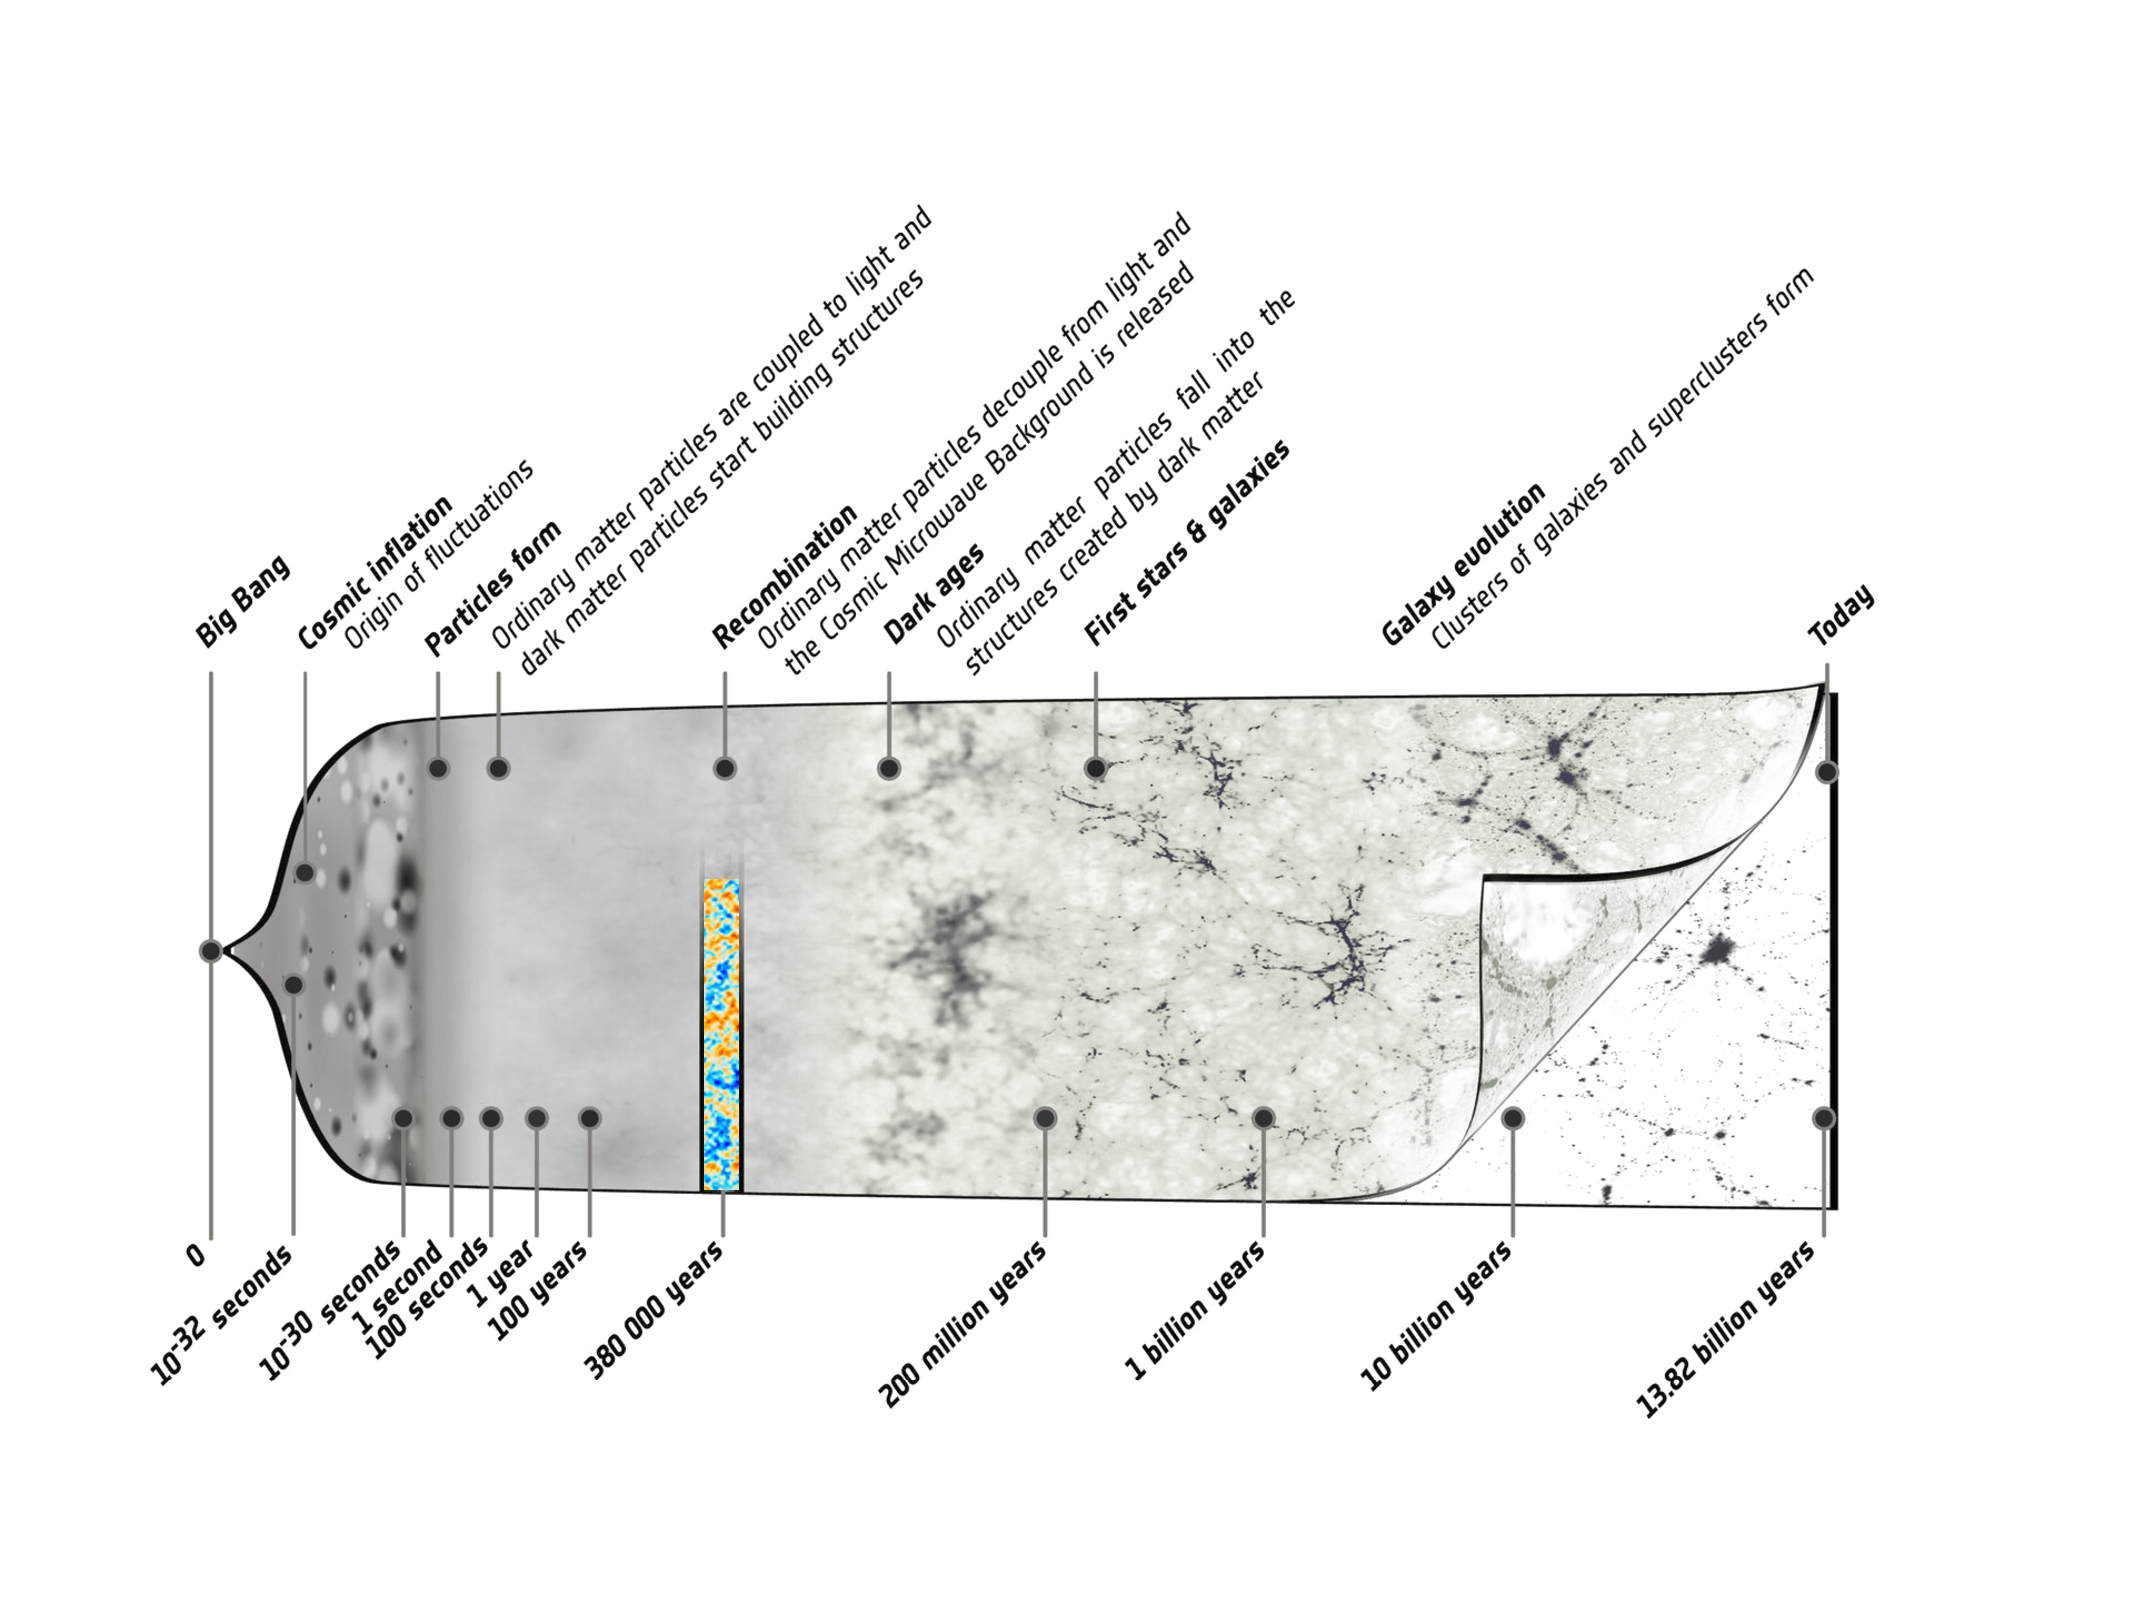
\includegraphics[width=.9\linewidth, trim={2cm 3cm 2cm 3cm}, clip]{Figures/Chap_cosmo/history_of_Universe.pdf}
    \caption{
        Résumé des étapes de l'histoire thermique de l'Univers, du Big Bang à aujourd'hui.
        Crédit: \href{https://www.esa.int/ESA_Multimedia/Images/2013/03/Planck_history_of_Universe_zoom}{ESA – C. Carreau}
    }
    \label{fig:cosmo:thermal_history}
\end{figure*}

% ===================================================================================== %
\section{Origine des grandes structures}\label{sec:struct_form}

Les équations de Friedmann permettent l'étude de la dynamique d'un univers homogène et isotrope.
La faible amplitude des fluctuations en température du CMB nous confirme l'isotropie à grande échelle de l'Univers.
Cependant, l'Univers contemporain est hautement hétérogène aux petites échelles, comme en témoigne l'existence de structures telles que les galaxies, amas de galaxies, étoiles et autres astres.
Notre Univers est donc homogène aux grandes échelles et hétérogène aux petites, ce qui n'est pas expliqué par le modèle standard de la cosmologie.
Nous décrivons dans cette section le paradigme inflationnaire, permettant de pallier aux lacunes du modèle standard, et offrant un cadre théorique pouvant expliquer l'origine de la formation des grandes structures de l'Univers.

% ------------------------------------------------------------------------------------- %
\subsection{Limitations du modèle standard de la cosmologie}

Bien que capable d'expliquer une grande variété de phénomènes observés dans l'Univers, le modèle $\Lambda\mathrm{CDM}$ est limité et ne fournit pas de réponse à certaines questions fondamentales de la cosmologie, parmi lesquelles:

%\subsubsection{Origine de l'accélération contemporaine} % ----------------------------- %
%Nous avons vu en \mypageref{sec:dark_energy} que l'Univers était actuellement dans une phase d'expansion accélérée, et que celle-ci pouvait s'expliquer par la présence d'énergie sombre dominant l'Univers contemporain.
%Cependant, il n'existe à ce jour pas d'explication sur la nature de cette énergie.

\subsubsection{Le problème de l'homogénéité à grande échelle} % ----------------------- %
Les observations des anisotropies en température du fond diffus cosmologique nous indiquent que l'Univers était extraordinairement homogène au moment de son découplage 380 000 ans après le Big Bang, avec des fluctuations quatre ordres de grandeurs plus faibles que sa température moyenne.
Cette homogénéité peut s'expliquer par un équilibre thermique dans le plasma primordial.
Cependant, un tel équilibre requiert un contact causal entre les différentes régions de l'Univers, contact n'ayant pu exister au moment de l'émission du CMB au vu de la valeur du facteur d'échelle à cette époque.
Quantitativement, alors que le CMB est homogène sur tout le ciel (et donc pour des points séparés par des angles allant jusqu'à 180\textdegree), l'angle tendu par le rayon d'horizon de Hubble à cette époque est de l'ordre du degré.
Le modèle standard de la cosmologie ne permet donc pas d'expliquer l'homogénéité en température du fond diffus cosmologique.

\subsubsection{Le problème de l'hétérogénéité à petite échelle} % --------------------- %
Bien que remarquablement homogène à grande échelle, l'Univers est très hétérogène à petite échelle.
Le modèle cosmologique standard ne permet d'expliquer que partiellement ce constat: de faibles inhomogénéités dans l'Univers primordial peuvent croître avec l'expansion jusqu'à devenir les structures que nous connaissons.
Cependant, l'origine des fluctuations de densité primordiales nécessaires à ce développement n'est pas expliquée par le modèle cosmologique standard.

\subsubsection{Le problème de la platitude} % ----------------------------------------- %
Les analyses cosmologiques récentes, basées sur l'exploitation de différentes sondes, s'accordent à dire que la géométrie de l'Univers est extrêmement plate, correspondant à une densité d'énergie dans l'Univers très proche de la densité critique (équation \ref{eq:rho_crit}).
Une courbure aussi faible que celle mesurée par l'analyse des anisotropies du CMB avec \textit{Planck} ($\Omega_{k,0} \sim 10^{-3}$) nécessite une courbure inférieure à $10^{-60}$ à l'issue de l'ère de Planck\footnote{Premières $10^{-43}$ secondes de l'Univers.}.
Des contraintes aussi fortes requièrent donc un ajustement fin des propriétés physiques de l'Univers primordial pour qu'il puisse se développer en l'Univers contemporain que nous observons, sans que le modèle cosmologique standard n'offre d'explication.

% ------------------------------------------------------------------------------------- %
\subsection{Fluctuations primordiales et inflation}

Les problèmes d'homogénéité à grande échelle et de platitude peuvent être résolus par un même mécanisme: l'inflation.
Dans ce scénario, l'Univers primordial a subi une phase d'expansion accélérée très rapide, caractérisée par $\ddot{a} > 0$, soit:
\begin{equation}
    \frac{\d}{\d t} \frac{1}{aH} < 0
\end{equation}
La présence de faibles hétérogénéités dans l'Univers primordial, à l'origine du processus de formation des structures, peut également être expliquée dans ce cadre.

Le paradigme de l'inflation comprend un grand nombre de modèles visant à expliquer l'origine de l'expansion accélérée dans l'Univers primordial.
Dans sa forme la plus simple, l'inflation est due à un champ scalaire homogène $\varphi$ nommé \textit{inflaton}, faiblement couplé et de potentiel $V(\varphi)$, dont la densité d'énergie domine celles de la matière et du rayonnement dans l'Univers primordial, avant de s'effondrer.
Le Lagrangien de ce champ s'écrit
\begin{equation}
    \mathcal{L} = \frac{1}{2} \partial^\mu\varphi \, \partial_\mu\varphi - V(\varphi) = \frac{\dot{\varphi}^2}{2} - V(\varphi),
\end{equation}
et le tenseur énergie-impulsion de ce champ $T^{\mu\nu} = \partial^\mu\varphi \, \partial^\nu\varphi - \mathcal{L}g^{\mu\nu}$ prend alors la forme de celui d'un fluide parfait dont la densité et la pression s'écrivent
\begin{align}
    \label{eq:infla_dens_press}
    \nonumber \rho_\varphi c^2 &= \frac{\dot{\varphi}^2}{2} + V(\varphi)
    + \frac{1}{2}\left(\frac{\nabla\varphi}{a}\right)^2, \\
    %\qquad
    p_\varphi &= \frac{\dot{\varphi}^2}{2} - V(\varphi)
    - \frac{1}{6}\left(\frac{\nabla\varphi}{a}\right)^2.
\end{align}
Dans une phase d'expansion rapide de l'Univers (comme au cours du \textit{slow-roll} discuté dans le paragraphe suivant), les termes proportionnels au gradient du champ d'inflaton $\nabla\varphi$ deviennent rapidement négligeables, du fait de la présence au dénominateur du facteur d'échelle.
La conservation du tenseur énergie-impulsion donne alors l'équation du mouvement de ce champ:
\begin{equation}
    \label{eq:infla_mvt}
    \ddot{\varphi} + 3H\dot{\varphi} + \frac{\d V(\varphi)}{\d\varphi} = 0.
\end{equation}

On peut alors distinguer deux régimes.
Dans le cas où $\ddot{\varphi}$ est négligeable devant les autres termes, l'énergie potentielle du champ d'inflaton domine son énergie cinétique: on dit que le champ se trouve dans une phase de \textit{slow-roll}\footnote{L'équation du mouvement (\ref{eq:infla_mvt}) est similaire à celle d'une balle dévalant une colline avec une friction non-nulle. Le \textit{slow-roll} correspond au roulement initial, où la friction domine et ralentit le mouvement -- voir figure \ref{fig:inflation}, panneau gauche.}.
On peut alors écrire $\dot{\varphi}^2 \ll V(\varphi)$, et le rapport de la densité d'énergie et de la pression du champ d'inflaton (équation \ref{eq:infla_dens_press}) donne un paramètre d'équation d'état $w_\varphi = -1$, caractéristique d'une expansion accélérée de l'Univers.
À l'inverse, si le terme cinétique domine par rapport au potentiel, l'équation du mouvement est celle d'un oscillateur harmonique amorti, et le champ se trouve dans une phase de \textit{reheating}.
Dans cette phase, l'oscillation du champ d'inflaton permet de convertir son énergie par production de particules élémentaires (\eg\ \cite{abbott_particle_1982,albrecht_reheating_1982}).

Le comportement de l'inflaton est illustré en figure \ref{fig:inflation}.
S'il se trouve dans une région de potentiel élevé, il se dirigera vers un potentiel plus faible en \textit{slow-roll}, générant l'inflation dans la région grisée.
Une fois proche d'un minimum de potentiel, le champ se trouvera dans une phase d'oscillations périodiques amorties avant de se stabiliser, mettant un terme à l'inflation.

\begin{figure*}[t]
    \centering
    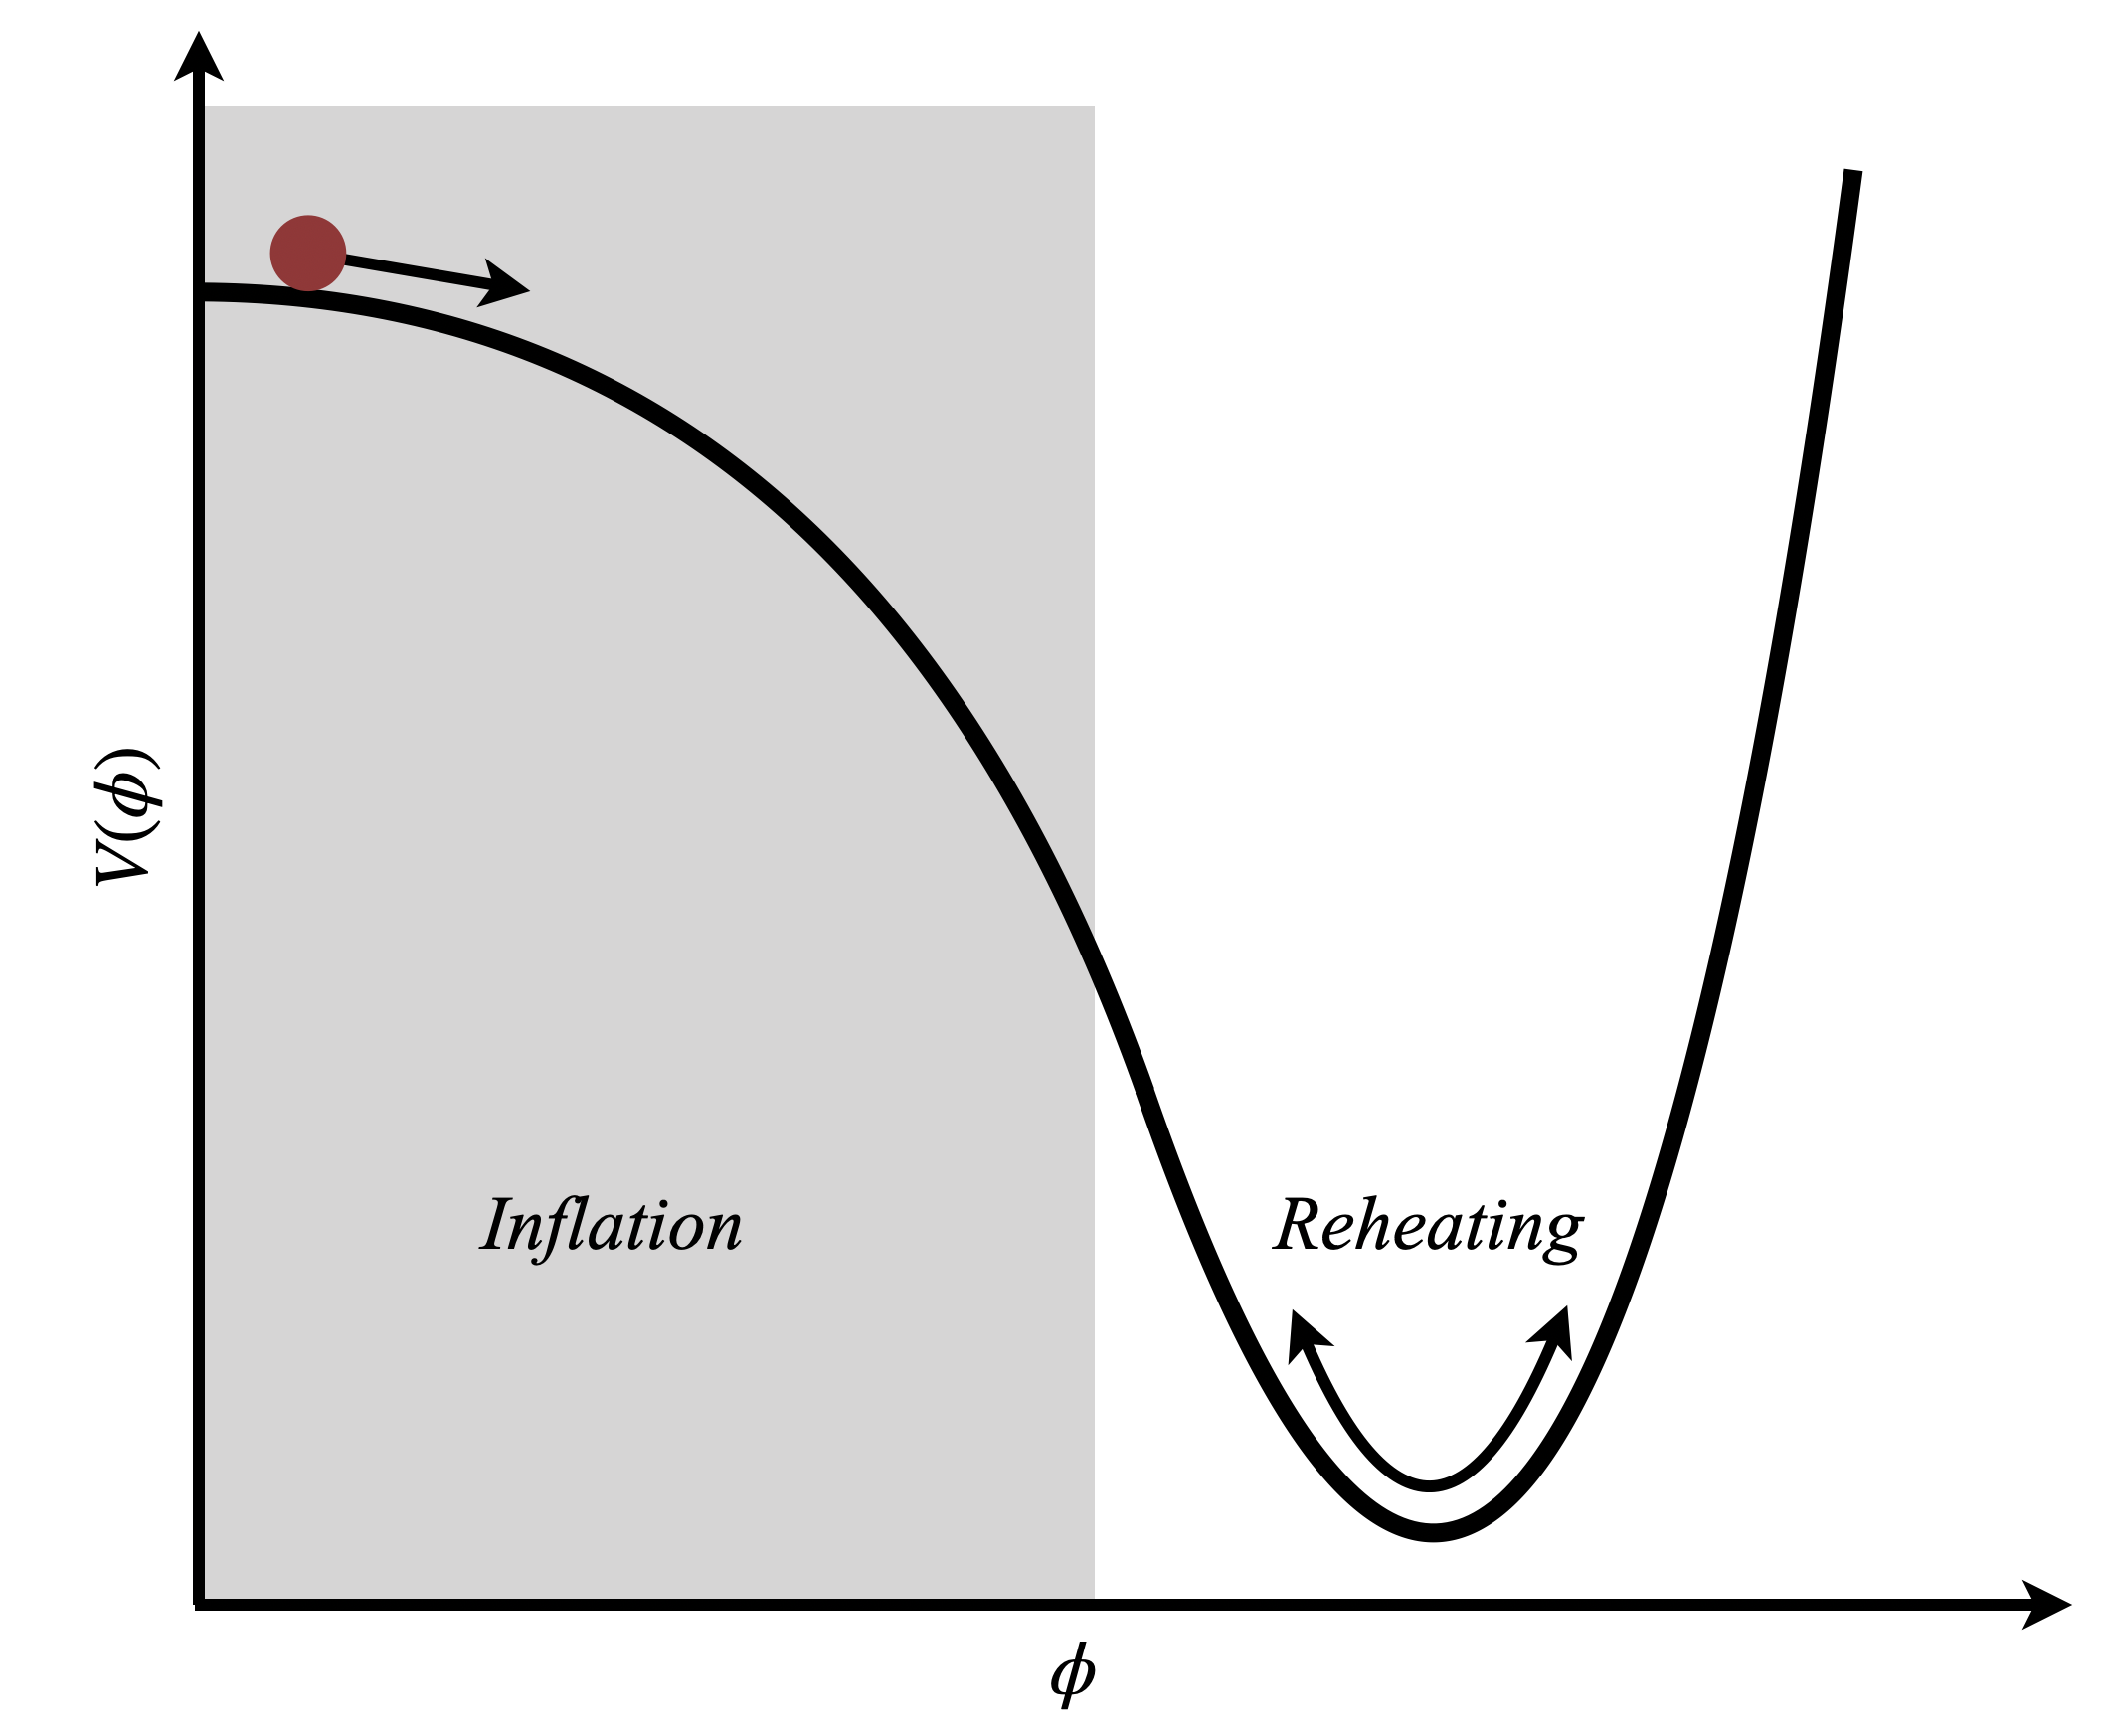
\includegraphics[height=6.6cm]{Figures/Chap_cosmo/SlowRoll2.png}\hfill
    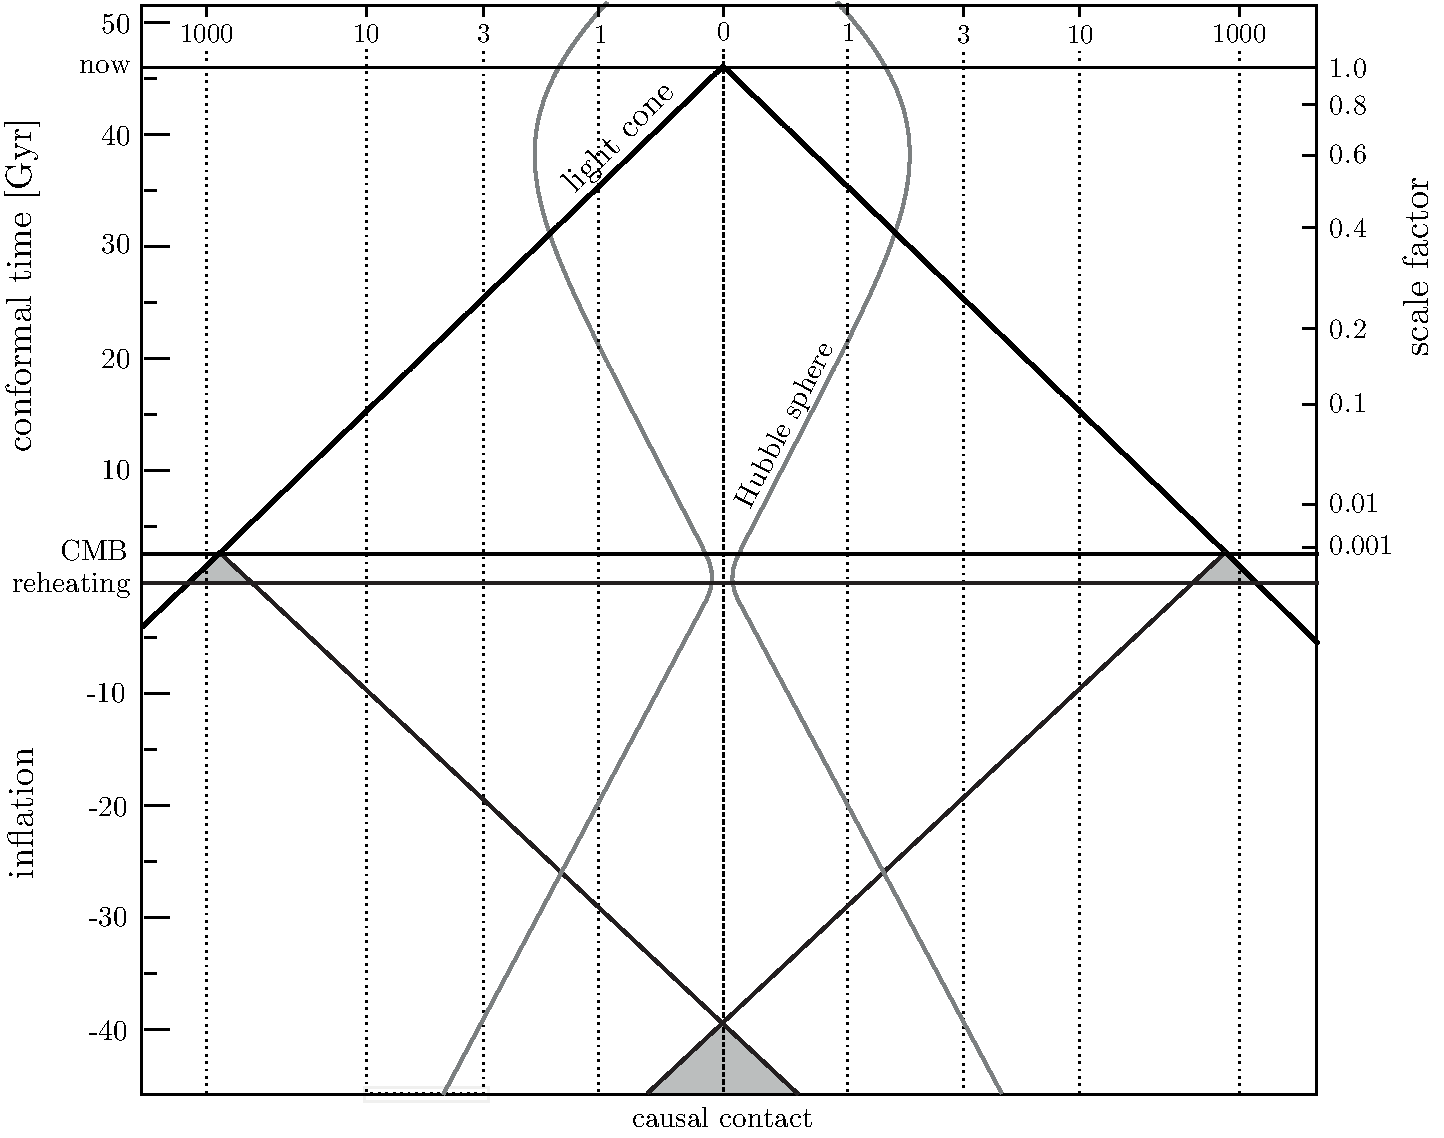
\includegraphics[height=6.6cm]{Figures/Chap_cosmo/spacetime_inflation.pdf}
    \caption{
        \textbf{Gauche:} Exemple de comportement du champ d'inflaton illustrant les deux régimes de l'équation (\ref{eq:infla_mvt}): le champ commence en \textit{slow roll} dans une région de potentiel élevé, puis se stabilise dans une région de bas potentiel, avec des oscillations rapides correspondant au \textit{reheating}.
        \textbf{Droite:} Diagramme d'espace-temps illustrant le contact causal de régions opposées dans le CMB au début de l'inflation.
        Figure extraite de \cite{baumann_inflation_2015}.
    }
    \label{fig:inflation}
\end{figure*}

La dynamique de l'inflation permet de comprendre la raison pour laquelle elle résout les problèmes de la platitude, de l'horizon et de l'hétérogénéité.
La densité d'énergie correspondant à la courbure de l'Univers étant définie par $\Omega_k = -kc^2 / (aH)^2$, celle-ci diminue rapidement avec le facteur d'échelle.
Quantitativement, en introduisant le nombre de \textit{e-folds} $N_e$, quantifiant l'augmentation du facteur d'échelle au cours de la phase inflationnaire, comme
\begin{equation}
    N_e = \ln \frac{a_f}{a_i} = \int_{t_i}^{t_f} H(t) \d t,
\end{equation}
il aparaît que $N_e \sim 60$ permet de passer d'une courbure $\Omega_k \sim 1$ au début de l'inflation à $\Omega_k \sim 10^{-60}$ à son issue, condition requise pour observer une courbure actuelle aussi faible que celle mesurée par le satellite \textit{Planck}.
De plus, le rayon de Hubble diminue pendant la phase inflationnaire, permettant à des points diamétralement opposés dans le CMB d'avoir été en contact causal.
Cela permet donc d'expliquer l'homogénéité du CMB, comme illustré sur le panneau droit de la figure \ref{fig:inflation}.

Enfin, le champ d'inflaton permet de comprendre l'origine des fluctuations de densité dans l'Univers primordial: considérons des fluctuations quantiques du champ comme une perturbation au premier ordre, soit
\begin{equation}
    \varphi(\xt) = \bar{\varphi}(t) + \delta\varphi(\xt),
\end{equation}
où $\bar{\varphi}(t)$ est la valeur moyenne du champ dans l'espace, ne dépendant que du temps dans l'hypothèse d'homogénéité. \\
Il apparait alors que la valeur du champ et de son potentiel ne sont pas égales en tout point de l'espace.
%On peut introduire le spectre de puissance des fluctuations de $\varphi$ comme la transformée de Fourier de sa fonction de corrélation à deux points $\xi_{\delta\varphi}(\vec{x})$:
%\begin{equation}
%    \label{eq:infla_pk}
%    P_{\delta\varphi}(k) = \int \xi_{\delta\varphi}(\vec{x}) e^{-i \vec{k} \cdot \vec{x}} \, \d^3 \vec{x}.
%\end{equation}
En vertu du lien entre densité d'énergie et espace-temps décrit par les équations d'Einstein (\ref{eq:einst_field}), ces inhomogénéités créent des perturbations dans la métrique de l'Univers, qui génèrent à leur tour des fluctuations dans la densité d'énergie du plasma primordial.
Ainsi, en plus des problèmes de l'horizon et de la platitude, l'inflation offre une origine au processus de formation des structures, qui sera détaillée dans la section suivante.

% ===================================================================================== %
\section{Évolution des grandes structures}

% ------------------------------------------------------------------------------------- %
\subsection{Croissance des inhomogénéités de densité}

Nous avons vu dans la section précédente comment l'inflation permettait de générer des fluctuations de densité dans l'Univers primordial.
Celles-ci seront ensuite amplifiées au cours de l'évolution de l'Univers par effondrement gravitationnel de la matière vers les régions les plus denses.
Ce processus de formation des structures est à l'origine des galaxies et de la distribution à grande échelle de la matière dans l'Univers contemporain, formant la toile cosmique.
Cette section détaille ce formalisme dans le but de comprendre l'origine des amas de galaxies, qui constituent la sonde cosmologique étudiée dans cette thèse.

Dans le régime linéaire, les fluctuations de densité issues de l'inflation peuvent s'écrire comme une perturbation au premier ordre de la densité moyenne,
\begin{equation}
    \label{eq:contrast}
    \rho(\xt) = \bar{\rho}(t) \left[1 + \delta(\xt) \right],
\end{equation}
où $\bar{\rho}(t)$ est la densité moyenne de l'Univers, $\vec{x}$ les coordonnées comobiles\footnotemark\ tri-dimensionelles, et $\delta(\xt)$ est appelé le paramètre de contraste. \\
\footnotetext{Le système de coordonnées comobiles se dilate avec le temps suivant l'expansion de l'Univers.}
La densité moyenne de l'Univers ne dépend que du temps, traduisant l'hypothèse d'un univers homogène à grande échelle et hétérogène seulement aux petites échelles.
Le fluide parfait comobile composant l'Univers doit alors satisfaire aux équations d'Euler, de la continuité, et de Poisson:
\begin{equation}
    \pdv{\vec{v}}{t} + (\vec{v} \cdot \vec{\nabla}) \vec{v} = -\vec{\nabla}\varphi - \frac{\vec{\nabla}p}{\rho} \label{eq:cosmo:euler}
\end{equation}
\begin{equation}
    \pdv{\rho}{t} + \vec{\nabla} \cdot (\rho \vec{v}) = 0 \label{eq:cosmo:conti}
\end{equation}
\begin{equation}
    \nabla^2 \Phi = 4\pi G \rho \label{eq:cosmo:poisson}
\end{equation}
où $p$ est la pression des fluides, $\vec{v}$ leur vitesse, et $\Phi$ le potentiel gravitationnel. \\
En injectant l'expression de la densité perturbée (\ref{eq:contrast}) dans ces équations, et en les combinant, on trouve l'expression de l'évolution des perturbations dans le temps:
\begin{equation}
    \pdvsq{\delta(\xt)}{t} + 2H(t)\pdv{\delta(\xt)}{t} = \left[4\pi G \bar{\rho}(t) + \frac{c_s^2}{a^2} \nabla^2\right] \delta(\xt),
\end{equation}
où $c_s$ est la vitesse du son dans le fluide. \\
Dans l'espace de Fourier, et en définissant $\delta_k {\rm sin}(\vec{k}\cdot\vec{r}) = \delta(\xt)$, cette équation prend la forme
\begin{equation}
    \ddot{\delta}_k + 2H\dot{\delta}_k = \left[4\pi G \bar{\rho} - \frac{c_s^2}{a^2} k^2\right] \delta_k
\end{equation}
ou encore, en introduisant l'échelle de Jeans $\lambda_{\rm J} \equiv c_s / \sqrt{\pi / G\bar{\rho}}$ et le mode associé $k_{\rm J} =2\pi a/\lambda_{\rm J}$, %= a/c_s \times \sqrt{4\pi G \bar{\rho}}$,
\begin{equation}
    \label{eq:cosmo:delta_k}
    \ddot{\delta}_k + 2H\dot{\delta}_k = \frac{c_s^2}{a^2} (k_{\rm J}^2 - k^2) \delta_k.
\end{equation}

Deux régimes asymptotiques apparaissent.
Pour les perturbations plus grandes que l'échelle de Jeans, soit $k^2 \ll k_{\rm J}^2$, la gravitation domine l'évolution des perturbations, et leur croissance est permise.
À l'inverse, lorsque $k^2 \gg k_{\rm J}^2$, la pression domine l'effondrement gravitationnel et la croissance des perturbations est atténuée.
Ainsi, lorsque la densité d'énergie est partagée entre matière et rayonnement (dans l'Univers primordial, à $z \lesssim 3000$), les inhomogénéités de densité oscillent, augmentant sous domination de la force gravitationnelle, puis diminuant lorsque cette dernière devient faible devant les forces de pression.
Ce mécanisme empêche le développement des inhomogénéités au cours de l'ère du rayonnement. %, et est à l'origine des oscillations acoustiques de baryons (BAO) qui constituent aujourd'hui l'une des sondes majeures utilisées en cosmologie observationnelle (voir \cite{weinberg_observational_2013,aubourg_cosmological_2015} pour des revues).

Lorsque la matière domine la densité d'énergie de l'Univers, soit $a(t) \propto t^{2/3}$ d'après l'équation de Friedmann (\ref{eq:fried1}), les forces de pression deviennent négligeables, autorisant la croissance des inhomogénéités et la formation des structures.
La résolution de l'équation (\ref{eq:cosmo:delta_k}) montre alors que le contraste augmente comme $\delta(t) \propto t^{2/3}$.
Plus tard, lors de la domination de l'énergie sombre, le facteur d'échelle croît comme $a(t) \propto {\rm exp}(Ht)$, et la résolution de (\ref{eq:cosmo:delta_k}) montre une diminution du paramètre de contraste comme $\delta(t) \propto {\rm exp}(-2Ht)$.

% ------------------------------------------------------------------------------------- %
\subsection{Spectre de puissance de la distribution de matière}

Comme nous l'avons vu dans la section précédente, la distribution de densité de l'Univers primordial résulte d'un processus aléatoire, et la structure de l'Univers contemporain du développement de ces inhomogénéités.
Dans le cas de fluctuations gaussiennes, la distribution de densité primordiale peut se résumer à la fonction de corrélation du paramètre de contraste,
\begin{equation}
    \xi(\vec{r}) = \left< \delta(\vec{x} + \vec{r}) \delta(\vec{r}) \right>,
\end{equation}
où $\left< \cdots \right>$ représente la valeur moyenne prise en toute position $\vec{x}$ de l'Univers. \\
On peut encore définir le spectre de puissance primordial $P_{\rm prim.}(k)$ comme la transformé de Fourier de cette fonction de corrélation, %ou bien sous la forme:
\begin{equation}
    %\Delta^2(k) \equiv \frac{k^3}{2\pi^2} P(k) = \frac{k^3}{2\pi^2} \int \xi(\vec{r}) e^{-i \vec{k} \cdot \vec{r}} \, \d^3 \vec{r}.
    P_{\rm prim.}(k) = \int \xi(\vec{r}) e^{-i \vec{k} \cdot \vec{r}} \, \d^3 \vec{r}.
\end{equation}
Les contraintes observationnelles sur le spectre de puissance primordial, obtenues notamment à partir de l'analyse des anisotropies du CMB, favorisent une forme en loi de puissance de ce dernier, soit $P(k) \propto k^n$, avec $n \simeq 1$ \cite{planck_collaboration_planck_2020}.
Le cas où $n = 1$ donne le spectre dit de Harrison-Zeldovich \cite{harrison_fluctuations_1970,zeldovich_hypothesis_1972}, qualifié d'invariant d'échelle.
En effet, en vertu de l'équation de Poisson, un spectre de puissance de la densité de matière de la forme $P(k) \propto k$ mène à un spectre de puissance du potentiel gravitationnel plat.

Dans l'Univers contemporain, les inhomogénéités de densité proviennent de l'accroissement des fluctuations primordiales.
Le spectre de puissance de la distribution de matière observable à un redshift $z$ est donc étroitement lié au spectre de puissance primordial, à travers
\begin{equation}
    P(z, k) = P_{\rm prim.}(k) \times T^2(z, k),
\end{equation}
où $T(z, k)$ est la fonction de transfert caractérisant l'évolution des perturbations. \\
La variance de la distribution de matière dans une sphère de rayon $r$ à un redshift $z$ est alors donnée par:
\begin{equation}
    \label{eq:matter_fluct}
    \sigma^2(z, r) = \frac{1}{(2\pi)^3} \int W(kr) P(z, k) \, \d^3k,
\end{equation}
où $W(kr)$ est la fonction fenêtre utilisée pour lisser la distribution de matière; par exemple, la fonction \textit{top-hat} considérant une sphère de rayon $r$,
\begin{equation}
    \label{eq:tophat}
    W(kr) = 3 \frac{\sin kr}{(kr)^3} - 3 \frac{\cos kr}{(kr)^2}.
\end{equation}
L'équation (\ref{eq:matter_fluct}) permet de définir le paramètre cosmologique $\sigma_8$ comme l'amplitude moyenne des fluctuations dans une sphère de $8 \, h^{-1}\, {\rm Mpc}$, soit
\begin{equation}
    \label{eq:sigma8}
    \sigma_8 = \sqrt{\sigma^2(z=0, r=8 \, h^{-1}\, {\rm Mpc})}.
\end{equation}
Ce paramètre a été mesuré par l'analyses des anisotropies primaires du CMB vues par \textit{Planck} à une valeur de $\sigma_8 = 0.8102 \pm  0.006$ \cite{planck_collaboration_planck_2020}.
Nous discuterons des différentes mesures obtenues par d'autres sondes en \mypageref{sec:current_surveys}.

% ------------------------------------------------------------------------------------- %
\subsection{Fonction de masse et distribution de halos}\label{sec:cosmo_hmf}

Le formalisme développé jusqu'ici repose sur l'hypothèse de linéarité des inhomogénéités du champ de matière primordial: d'après l'équation (\ref{eq:contrast}), les surdensités représentent des perturbations au premier ordre d'un Univers globalement homogène.
Cette hypothèse suppose donc que $\delta \ll 1$, condition non-remplie dans les surdensités de l'Univers contemporain.
Par exemple, les amas de galaxies peuvent aujourd'hui atteindre des densités centrales de l'ordre de $\sim 10^{-22} \;{\rm kg \cdot m^{-3}}$, correspondant à un contraste de l'ordre de $10^4$.
La description de l'Univers contemporain par le seul formalisme de la croissance des structures par développement des inhomogénéités en régime linéaire est donc incomplète.

Les phénomènes physiques devant être pris en compte lors du traitement non-linéaire de la croissance des structures sont très riches, et font de ce formalisme un cadre complexe.
Une approche possible est la théorie de \myciteauthor{press_formation_1974}, dans laquelle l'hypothèse principale est le fait que l'intégralité de la matière est aujourd'hui contenue dans des halos sphériques à l'équilibre hydrostatique.
Dans le cadre de cette théorie, le nombre de halos de masse comprise dans un intervalle $[M, M + \d M]$ est donné par la fonction de masse $\d N / \d M$.
Dans sa formulation courante, formalisée par \myciteauthor{tinker_toward_2008}, celle-ci s'écrit à un redshift donné:
\begin{equation}
    \label{eq:hmf}
    \frac{\d N}{\d M} = f(\sigma) \frac{\bar{\rho}}{M} \left| \frac{\d \, {\rm ln}\, \sigma^{-1}}{\d M} \right|,
\end{equation}
où $\bar{\rho}$ est la densité moyenne de l'Univers, $\sigma$ la racine de la variance de la distribution de matière, reliée au spectre de puissance par l'équation (\ref{eq:matter_fluct}), et $f(\sigma)$ est la fonction de multiplicité dépendant de $\sigma$, par
\begin{equation}
    f(\sigma) = A \left[ 1 + \left(\frac{b}{\sigma}\right)^a \right] e^{-c / \sigma^2}
\end{equation}
Les valeurs des paramètres $(A, a, b, c)$ de la fonction de multiplicité sont donc des paramètres de la fonction de masse, et sont généralement mesurés dans des simulations numériques (\eg\ \cite{tinker_toward_2008,bocquet_halo_2016,bocquet_mira-titan_2020}).
Comme nous le verrons dans le chapitre suivant, la fonction de masse est un élément central des analyses cosmologiques basées sur les amas de galaxies.
En effet, elle dépend de la distribution de matière dans l'Univers, et donc des paramètres cosmologiques.

C'est cette dépendance, illustrée en figure \ref{fig:hmf_cosmo}, qui est exploitée pour contraindre la cosmologie à l'aide d'amas de galaxies.
Celle-ci montre l'évolution des valeurs de la fonction de masse de \myciteauthor{tinker_toward_2008} avec les paramètres $\Omega_m$ et $\sigma_8$.
On y observe que la fonction de masse croît avec $\Omega_m$: plus la matière est abondante dans l'Univers (c'est-à-dire plus $\Omega_m$ est grand), plus les halos, et donc les amas de galaxies, sont nombreux\footnotemark.
On y remarque également un comportement similaire pour $\sigma_8$: plus les fluctuations de la distribution de matière sont grandes (c'est-à-dire plus $\sigma_8$ est grand), plus les amas sont nombreux.
On note enfin que les deux paramètres cosmologiques ont une influence différente sur l'abondance d'amas.
Une variation de $\Omega_m$ influera principalement sur l'abondance d'amas de faible masse, alors qu'à l'inverse, une variation de $\sigma_8$ modifiera surtout l'abondance d'amas massifs.
Les contraintes basées sur l'abondance d'amas sont de fait sensibles à une combinaison des deux paramètres, pouvant varier d'une analyse à l'autre, et souvent exprimée par le paramètre $S_8$:
\begin{equation}
    S_8 \equiv \sigma_8 \sqrt{\Omega_m/0.3}.
\end{equation}
\footnotetext{Cette observation n'est plus vraie pour les objets extrêmement massifs, au delà de $2 \times 10^{15} \, M_\odot$ à $z=0.5$. On note que de tels objets sont des cas extrêmes; leur existence seule pousserait le modèle $\Lambda{\rm CDM}$ à ses limites, et des objets plus massifs pourrait même permettre de l'invalider -- voir par exemple \cite{harrison_consistent_2013}.}

La connaissance de la fonction de masse est donc une nécessité pour la justesse des analyses cosmologiques basées sur les statistiques d'amas (\eg\ \cite{salvati_impact_2020,artis_impact_2021}).
De telles analyses seront détaillées au chapitre suivant, et en particulier en section \mypageref{sec:cluster_nbcount}.

\begin{figure*}[t]
    \centering
    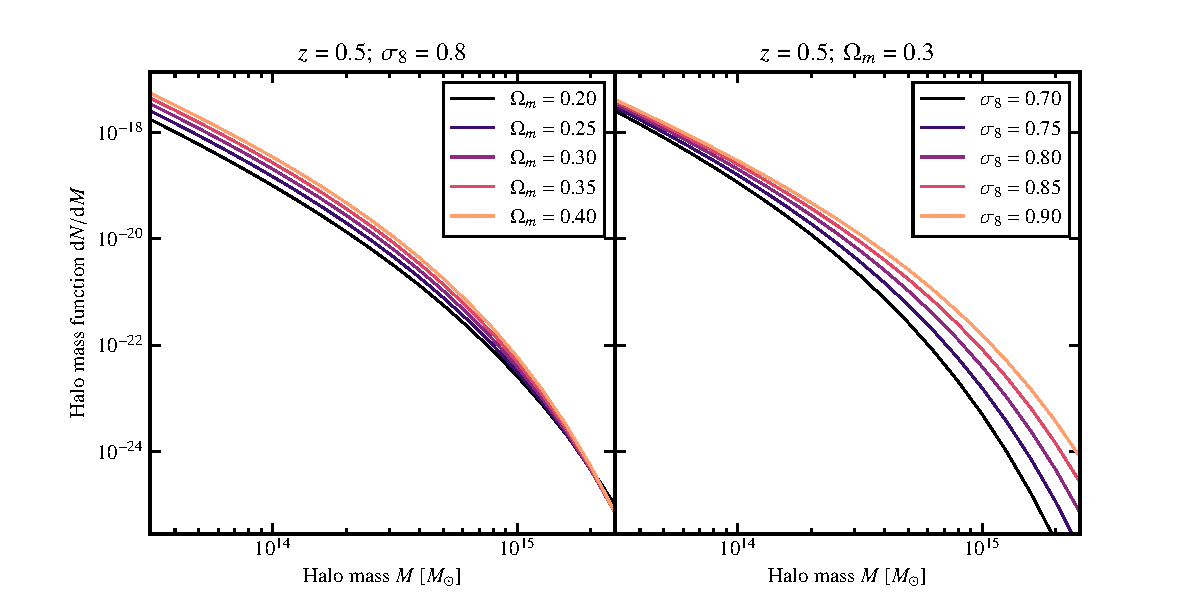
\includegraphics[width=\linewidth]{Figures/Chap_cosmo/hmf_cosmo.pdf}
    \caption{
        Illustration de l'évolution de la fonction de masse avec les paramètres cosmologiques.
        La fonction de masse de \myciteauthor{tinker_toward_2008} est représentée pour différentes valeurs de $\Omega_m$ (\textit{gauche}), et de $\sigma_8$ (\textit{droite}).
        Le redshift est fixé à $z = 0.5$.
    }
    \label{fig:hmf_cosmo}
\end{figure*}

% ===================================================================================== %
\section{Conclusions}

Le modèle standard de la cosmologie, accompagné du paradigme de l'inflation, fournit une description de l'Univers et de son évolution basée sur des hypothèses simples.
À l'heure actuelle, il est en remarquable accord avec les observations disponibles.
Cependant, plusieurs questions restent en suspens.
Par exemple, la nature de l'énergie sombre, cause de l'accélération récente de l'expansion, est une des énigmes non-résolues par le modèle $\Lambda {\rm CDM}$.
La mesure de son paramètre d'équation d'état, et de son éventuelle évolution dans le temps, peut apporter des réponses à cette question.

La mesure toujours plus précise des valeurs des paramètres cosmologiques est l'un des enjeux majeurs de la cosmologie moderne.
Dans ce but, la combinaison de plusieurs observables, nommées \textit{sondes cosmologiques}, s'impose comme un puissant moyen de mitiger les différentes incertitudes systématiques associées à chacune des sondes individuelles.
Plusieurs études récentes semblent indiquer un désaccord entre les mesures des paramètres cosmologiques effectués avec différentes sondes.
Par exemple, les mesures du taux actuel d'expansion de l'Univers $H_0$ réalisées par l'analyse des anisotropies du CMB sont en désaccord avec les mesures réalisées dans l'Univers contemporain (voir par exemple \cite{riess_large_2019,wong_h0licow_2020,efstathiou_h0_2021, freedman_measurements_2021}).
On note également la différence entre les estimations du paramètre $S_8$ par l'analyse du CMB et d'autres sondes, qui sera discutée au chapitre suivant.
Ces tensions peuvent être un signe de nouvelle physique, ou bien indiquer des effets systématiques non-maîtrisés.
Alors même que les incertitudes statistiques s'apprêtent à être réduites de manière conséquente avec les différents relevés cosmologiques du futur, ces systématiques deviendront de plus en plus importantes, et devront être étudiées afin de pouvoir répondre aux questions toujours ouvertes sur les propriétés les plus fondamentales de l'Univers.
Cette thèse s'inscrit dans le cadre de l'étude de ces effets systématiques dans l'exploitation cosmologique des amas de galaxies, qui sera décrite dans le chapitre suivant.


% ------------------------------------------- %
\chapter{Sonder la cosmologie à l'aide d'amas de galaxies}
\label{chap:amas}
\minitoc
Nous avons vu au chapitre \ref{chap:cosmo1} que la fonction de masse prédisait l'abondance de halos de matière sombre par unité de masse et de redshift.
Étant donné le lien étroit entre le processus de formation des structures et la cosmologie sous-jacente, on peut prédire que la fonction de masse dépend des propriétés de l'Univers et de son évolution depuis l'inflation.
Elle fait donc le lien entre la distribution de matière dans l'Univers et les paramètres cosmologiques à travers l'abondance de surdensités par unités de masse et de redshift.

C'est dans ce contexte que les amas de galaxies apparaissent comme une sonde cosmologique.
Ils constituent en effet les plus grandes structures gravitationnellement liées de l'Univers, et apparaissent comme l'aboutissement du processus de formation hiérarchique des structures.
Le nombre d'amas de galaxies observables dans le ciel est donc directement lié à la fonction de masse.
Par conséquent, un catalogue d'amas de galaxies de masse et redshift connus permet de   contraindre la fonction de masse, et donc les paramètres cosmologiques.

Ce chapitre décrit les éléments nécessaires à la réalisation de telles analyses.
Nous nous intéresserons tout d'abord à la définition des amas de galaxies et à leurs caractéristiques.
Nous discuterons ensuite des différentes observables des amas dans différentes longueurs d'onde, puis des contraintes cosmologiques par comptage d'amas de galaxies.
Nous terminerons par un tour d'horizon des résultats récents en cosmologie avec des amas de galaxies, et des perspectives de ce domaine.

% ===================================================================================== %
\section{Composition et masse des amas de galaxies}

% ------------------------------------------------------------------------------------- %
\subsection{Définition d'un amas de galaxies}

Les amas de galaxies représentent la dernière étape du processus de formation hiérarchique des structures développé dans la section \ref{sec:struct_form}, et constituent les plus grandes structures gravitationnellement liées de l'Univers.
Ils se forment par effondrement gravitationnel de la matière et par accrétion du milieu environnant autour des pics de densité de la toile cosmique, c'est-à-dire aux intersections de ses filaments.
Ils offrent donc un traceur de la distribution de matière dans l'Univers.
C'est la raison pour laquelle leur distribution en masse et en redshift constitue une sonde permettant d'étudier les processus de formation des structures, et donc la cosmologie sous-jacente.
Ce point sera abordé plus en détail en section \ref{sec:cluster_nbcount}.

La formation des amas de galaxies a lieu dans l'Univers contemporain, à des redshifts $z \lesssim 3$.
Les structures de plus haut redshift sont essentiellement représentées par des galaxies seules, ou par des groupes d'un petit nombre de galaxies, désignés comme proto-amas (voir par exemple \cite{zhou_goods-alma_2020}).

La composition des amas de galaxies est représentative de celle de la matière dans l'Univers (voir \eg\ \cite{pratt_galaxy_2019}).
Elle est dominée par la matière sombre, comptant pour $\sim$ 85 \% de leur masse.
La matière baryonique des amas est principalement contenue dans un gaz chaud ionisé nommé milieu intra-amas (ou ICM pour \textit{intracluster medium}), représentant $\sim$ 12 \% du contenu en masse des amas.
Ce gaz est principalement composé de noyaux légers et d'électrons libres, à des températures de l'ordre de $10^7 - 10^8 \;{\rm K}$.
Enfin, le reste de la matière baryonique des amas est contenu dans leurs galaxies, qui ne représentent qu'une faible fraction de la masse totale des amas ($\sim$ 3\%).

% ------------------------------------------------------------------------------------- %
\subsection{Masse et rayon des amas de galaxies} \label{sec:int_quant}

Les amas de galaxies sont des objets complexes et diffus par nature, auxquels il est difficile d'attribuer une taille physique.
Leur étude passe donc par la définition d'un rayon caractéristique à l'intérieur duquel leurs propriétés physiques seront étudiées.
Pour cela, le rayon de viriel peut être utilisé, décrivant un halo à l'équilibre.
En pratique, celui-ci est difficile à estimer, du fait des différents processus physiques perturbant leur équilibre, et de sa taille souvent plus grande que les champs couverts par les observations.
Par conséquent, il est plus utile de définir un rayon $R_\Delta$ par la valeur moyenne du contraste de densité $\Delta$ qu'il contient:
\begin{equation}
    \label{eq:cluster_contrast_R}
    \Delta \equiv \frac{\left<\rho(<R_\Delta)\right>}{\rho_{\rm crit}(z)},
\end{equation}
ce qui correspond à considérer l'amas comme une boule homogène de masse volumique $\Delta$ fois supérieure à la densité critique de l'Univers. \\
La valeur de contraste considérée est arbitraire; les valeurs usuelles sont $\Delta \in [200, 500, 2500]$, en fonction de la couverture angulaire des observations utilisées et des régions d'intérêt.
Des études portant sur les propriétés des amas dans $R_{2500}$ se focaliseront sur le cœur des amas, alors que des études à $R_{200}$ permettront des contraintes sur leur périphérie.
Au cours de cette thèse, nous utiliserons principalement $R_{500}$, valeur conventionnellement utilisée pour des études sur les régions intermédiaires des amas de galaxies et du milieu intra-amas.
Comme nous le verrons en section \mypageref{sec:current_surveys}, les amas de galaxies détectés par les instruments actuels ont des masses $M_{500}$ typiquement de l'ordre de $10^{14} - 10^{15} \;M_\odot$.

Parmi les propriétés fondamentales des amas de galaxies, leur masse joue un rôle crucial dans l'estimation de contraintes sur les paramètres cosmologiques.
La connaissance des masses individuelles d'un grand nombre d'amas de galaxies est en effet nécessaire aux études de comptage, qui constituent l'une des sondes cosmologiques majeures basées sur les amas de galaxies, et qui sera détaillée en section \ref{sec:cluster_nbcount}.

Plusieurs méthodes existent pour estimer la masse d'amas individuels; nous renvoyons le lecteur vers la revue récente de \myciteauthor{pratt_galaxy_2019} pour une liste détaillée des différentes possibilités ouvertes par les observations récentes d'amas de galaxies à différentes longueurs d'onde.
La mesure principale utilisée dans cette thèse repose sur la connaissance des propriétés thermodynamiques du milieu intra-amas, et sur l'hypothèse de l'équilibre hydrostatique.
Dans le cadre de cette hypothèse, les forces gravitationnelles subies par un élément de fluide sont compensées par les forces de pression:
\begin{equation}
    \frac{1}{\rho} \vec{\nabla} P = \vec{g} = \frac{-G M^{\rm HSE}}{r^2} \vec{u}_r,
\end{equation}
où $\vec{u}_r$ est un vecteur unitaire radial en coordonnées sphériques. \\
Alors, dans l'hypothèse de symétrie sphérique de l'amas, le profil de masse, soit la valeur de masse contenue dans une sphère de rayon $r$, s'écrit
\begin{equation}
    \label{eq:mhse}
    M^{\rm HSE}(<r) = \frac{-r^2}{G \mu m_{\rm p} n_\e(r)} \frac{\d P_\e}{\d r},
\end{equation}
où $\mu$ est le poids moléculaire moyen du milieu intra-amas, $\mu \equiv m/m_{\rm p}$; et $n_\e(r)$ et $P_\e(r)$ sont respectivement la densité et la pression des électrons du milieu intra-amas. \\
L'hypothèse de l'équilibre hydrostatique offre donc un estimateur du profil de masse des amas de galaxies.
La masse $M_\Delta$ contenue dans un rayon $R_\Delta$ peut alors être estimée grâce à la connaissance du profil de masse d'un amas de galaxies.
En effet, le rayon $R_\Delta$ peut être calculé en considérant une boule homogène de rayon $R_\Delta$ et de masse volumique $\rho_c(z)$, soit en résolvant:
\begin{equation}
    \label{eq:r_delta_from_m}
    \frac{M(<R_\Delta)}{\rho_c(z) \times \frac{4}{3} \pi R_\Delta^3} = \Delta.
\end{equation}
La valeur du profil de masse à ce rayon donne donc la masse $M_\Delta = M(<R_\Delta)$.
On note au passage la corrélation entre $R_\Delta$ et $M_\Delta$ par construction. Ce point revêt une importance capitale pour les mesures de relations d'échelle masse-observable, et sera discuté dans les chapitres \ref{chap:panco} et \ref{chap:scaling}.

La masse hydrostatique se présente donc comme un estimateur de la masse d'un amas reposant sur la mesure du profil de densité et de pression des électrons de l'ICM.
Comme nous le verrons par la suite, il est possible de mesurer ces propriétés grâce à l'émission des amas de galaxies en X et à l'observation de l'effet Sunyaev-Zeldovich.

% ------------------------------------------------------------------------------------- %
\subsection{Le biais hydrostatique}\label{sec:hse_bias}

La validité de l'hypothèse de l'équilibre hydrostatique dans les amas est le sujet de nombreuses études (\eg\ \cite{salvati_mass_2019}).
En effet, comme nous le verrons par la suite, les analyses cosmologiques par comptage d'amas sont limitées par la connaissance des masses des amas.
Une grande variété des processus physiques ayant lieu au sein de ces derniers (fusion de sous-structures, injection d'énergie par des noyaux actifs de galaxies) créent dans le milieu intra-amas des forces de pression non-thermiques.
Celles-ci ne sont en général pas contraintes par les observations, comme nous le verrons par la suite.
Les masses estimées par observation des propriétés thermodynamiques du milieu intra-amas peuvent donc souffrir d'un biais.
Celui-ci est nommé biais hydrostatique $b$, et permet de quantifier l'état de perturbation des amas:
\begin{equation}
    \label{eq:hse_bias}
    M^{\rm HSE} = (1-b)M^{\rm total}.
\end{equation}
On remarque alors que ce biais se propage au profil de masse hydrostatique discuté dans la section précédente, et donc au calcul du rayon caractéristique $R_\Delta$ décrit dans l'équation (\ref{eq:r_delta_from_m}).
La masse caractéristique $M_\Delta$ obtenue grâce au profil de masse hydrostatique est donc affectée de ce biais non-seulement de par la différence entre les profils de masse, mais également par la différence des rayons caractéristiques inférés.

La mesure du biais hydrostatique peut être réalisée par plusieurs moyens.
On peut étudier le biais à partir de simulations hydrodynamiques, dans lesquelles la masse réelle des amas est connue et la masse hydrostatique peut être calculée à partir de l'équation (\ref{eq:mhse}) (\eg\ \cite{barnes_characterizing_2021,gianfagna_exploring_2021}).
Cependant, cette approche suppose que les simulations sont parfaitement réalistes, et les résultats dépendent fortement de la modélisation des différents processus physiques inclus dans les simulations utilisées \cite{gianfagna_exploring_2021}.
Le biais hydrostatique peut également être étudié à partir d'observations.
En effet, il existe plusieurs estimateurs de masse des amas qui ne reposent pas sur l'hypothèse de l'équilibre hydrostatique.
Par exemple, les mesures de masse par effet de lentillage gravitationnel du CMB (\eg\ \cite{madhavacheril_atacama_2020, louis_calibrating_2017, zubeldia_cosmological_2019}) ou de galaxies d'arrière-plan\footnotemark (\eg\ \cite{sereno_comparing_2015}).
Les différents estimateurs de masse peuvent être comparés sur des échantillons d'amas afin de mesurer l'écart moyen entre les mesures de masse hydrostatique et celles ne reposant pas sur cette hypothèse.
\footnotetext{Plus de détails seront donnés en section \mypageref{sec:opt}.}

Une compilation de mesures de $(1-b)$ est présentée en figure \ref{fig:hse_bias}, montrant les différentes valeurs de biais obtenues par comparaison d'estimateurs de masse à partir d'observations et de simulations.
La région orange montre la valeur du biais hydrostatique obtenue par l'analyse cosmologique jointe des observations par \textit{Planck} de l'effet Sunyaev-Zeldovich et du CMB réalisée par \myciteauthor{salvati_constraints_2018}.
Une tension apparait: ce résultat est incompatible avec les mesures de biais réalisées par la comparaison de différents estimateurs de masse d'amas observés, à partir d'observations (points noirs) et de simulations (région violette).
S'il est à noter que cette différence a récemment été réduite par la réanalyse des observations du CMB par \textit{Planck}\footnotemark, la détermination de la valeur du biais hydrostatique reste l'un des enjeux majeurs de la cosmologie avec des amas de galaxies.
En effet, elle peut avoir un impact prononcé sur les mesures de paramètres cosmologiques, et une mauvaise estimation de $b$ entraîne un biais sur la mesure du paramètre $S_8$ (introduit en \ref{sec:cosmo_hmf}, et qui sera discuté en \ref{sec:current_surveys}).
\footnotetext{En particulier, la valeur de la profondeur optique jusqu'à la réionisation, $\tau$, a évolué entre les analyses de la collaboration \textit{Planck} en 2015 et 2018. Plus de détails peuvent être trouvés dans \cite{planck_collaboration_planck_2020}.}

\begin{SCfigure}[][t]
    \centering
    \includegraphics[width=.4\linewidth]{Figures/Chap_amas/b_salvati.eps}
    \hspace{15pt}
    \caption{
        Estimation du biais hydrostatique par comparaison de mesures de masse hydrostatique et par lentillage faible (voir section \ref{sec:opt}) pour différentes études (noir).
        La valeur nécessaire pour concilier les réultats du CMB et des amas de galaxies, mesurée par \cite{salvati_constraints_2018}, est indiquée en orange.
        La région violette représente les valeurs de $(1-b)$ permises par plusieurs analyses d'amas simulés \cite{planck_collaboration_planck_2013}.
        Figure extraite de \cite{salvati_constraints_2018}.
    }
    \label{fig:hse_bias}
\end{SCfigure}

% ===================================================================================== %
\section{Observations des amas de galaxies} \label{sec:cluster_obs}

La richesse des processus physiques ayant lieu au sein des amas de galaxies font de ceux-ci des objets multilongueur d'onde par nature, pouvant être détectés dans tous des domaines du spectre électromagnétique.
Dans cette section, nous présentons les longueurs d'onde principales utilisées pour la caractérisation des amas de galaxies, ainsi que les propriétés physiques des amas qu'elles permettent respectivement de sonder.
Une attention particulière sera portée à l'effet Sunyaev-Zeldovich, qui constitue l'observable principale étudiée au cours de cette thèse, en \ref{sec:sz}.

À titre d'illustration, les cartes d'un amas de galaxies dans les trois domaines de longueur d'onde discutés ici sont présentées en figure \ref{fig:macsj1149}.
On y voit que les amas apparaissent comme des objets diffus dans les observations dans les domaines millimétrique et X.
Comme nous le verrons par la suite, la raison en est que de telles observations cartographient le gaz du milieu intra-amas; c'est pourquoi la structure des amas à ces longueurs d'onde sont souvent similaires.
Les observations en visible des amas révèlent quant à elles la distribution des galaxies membres de l'amas.

\afterpage{
\begin{figure*}[t]
    \centering
    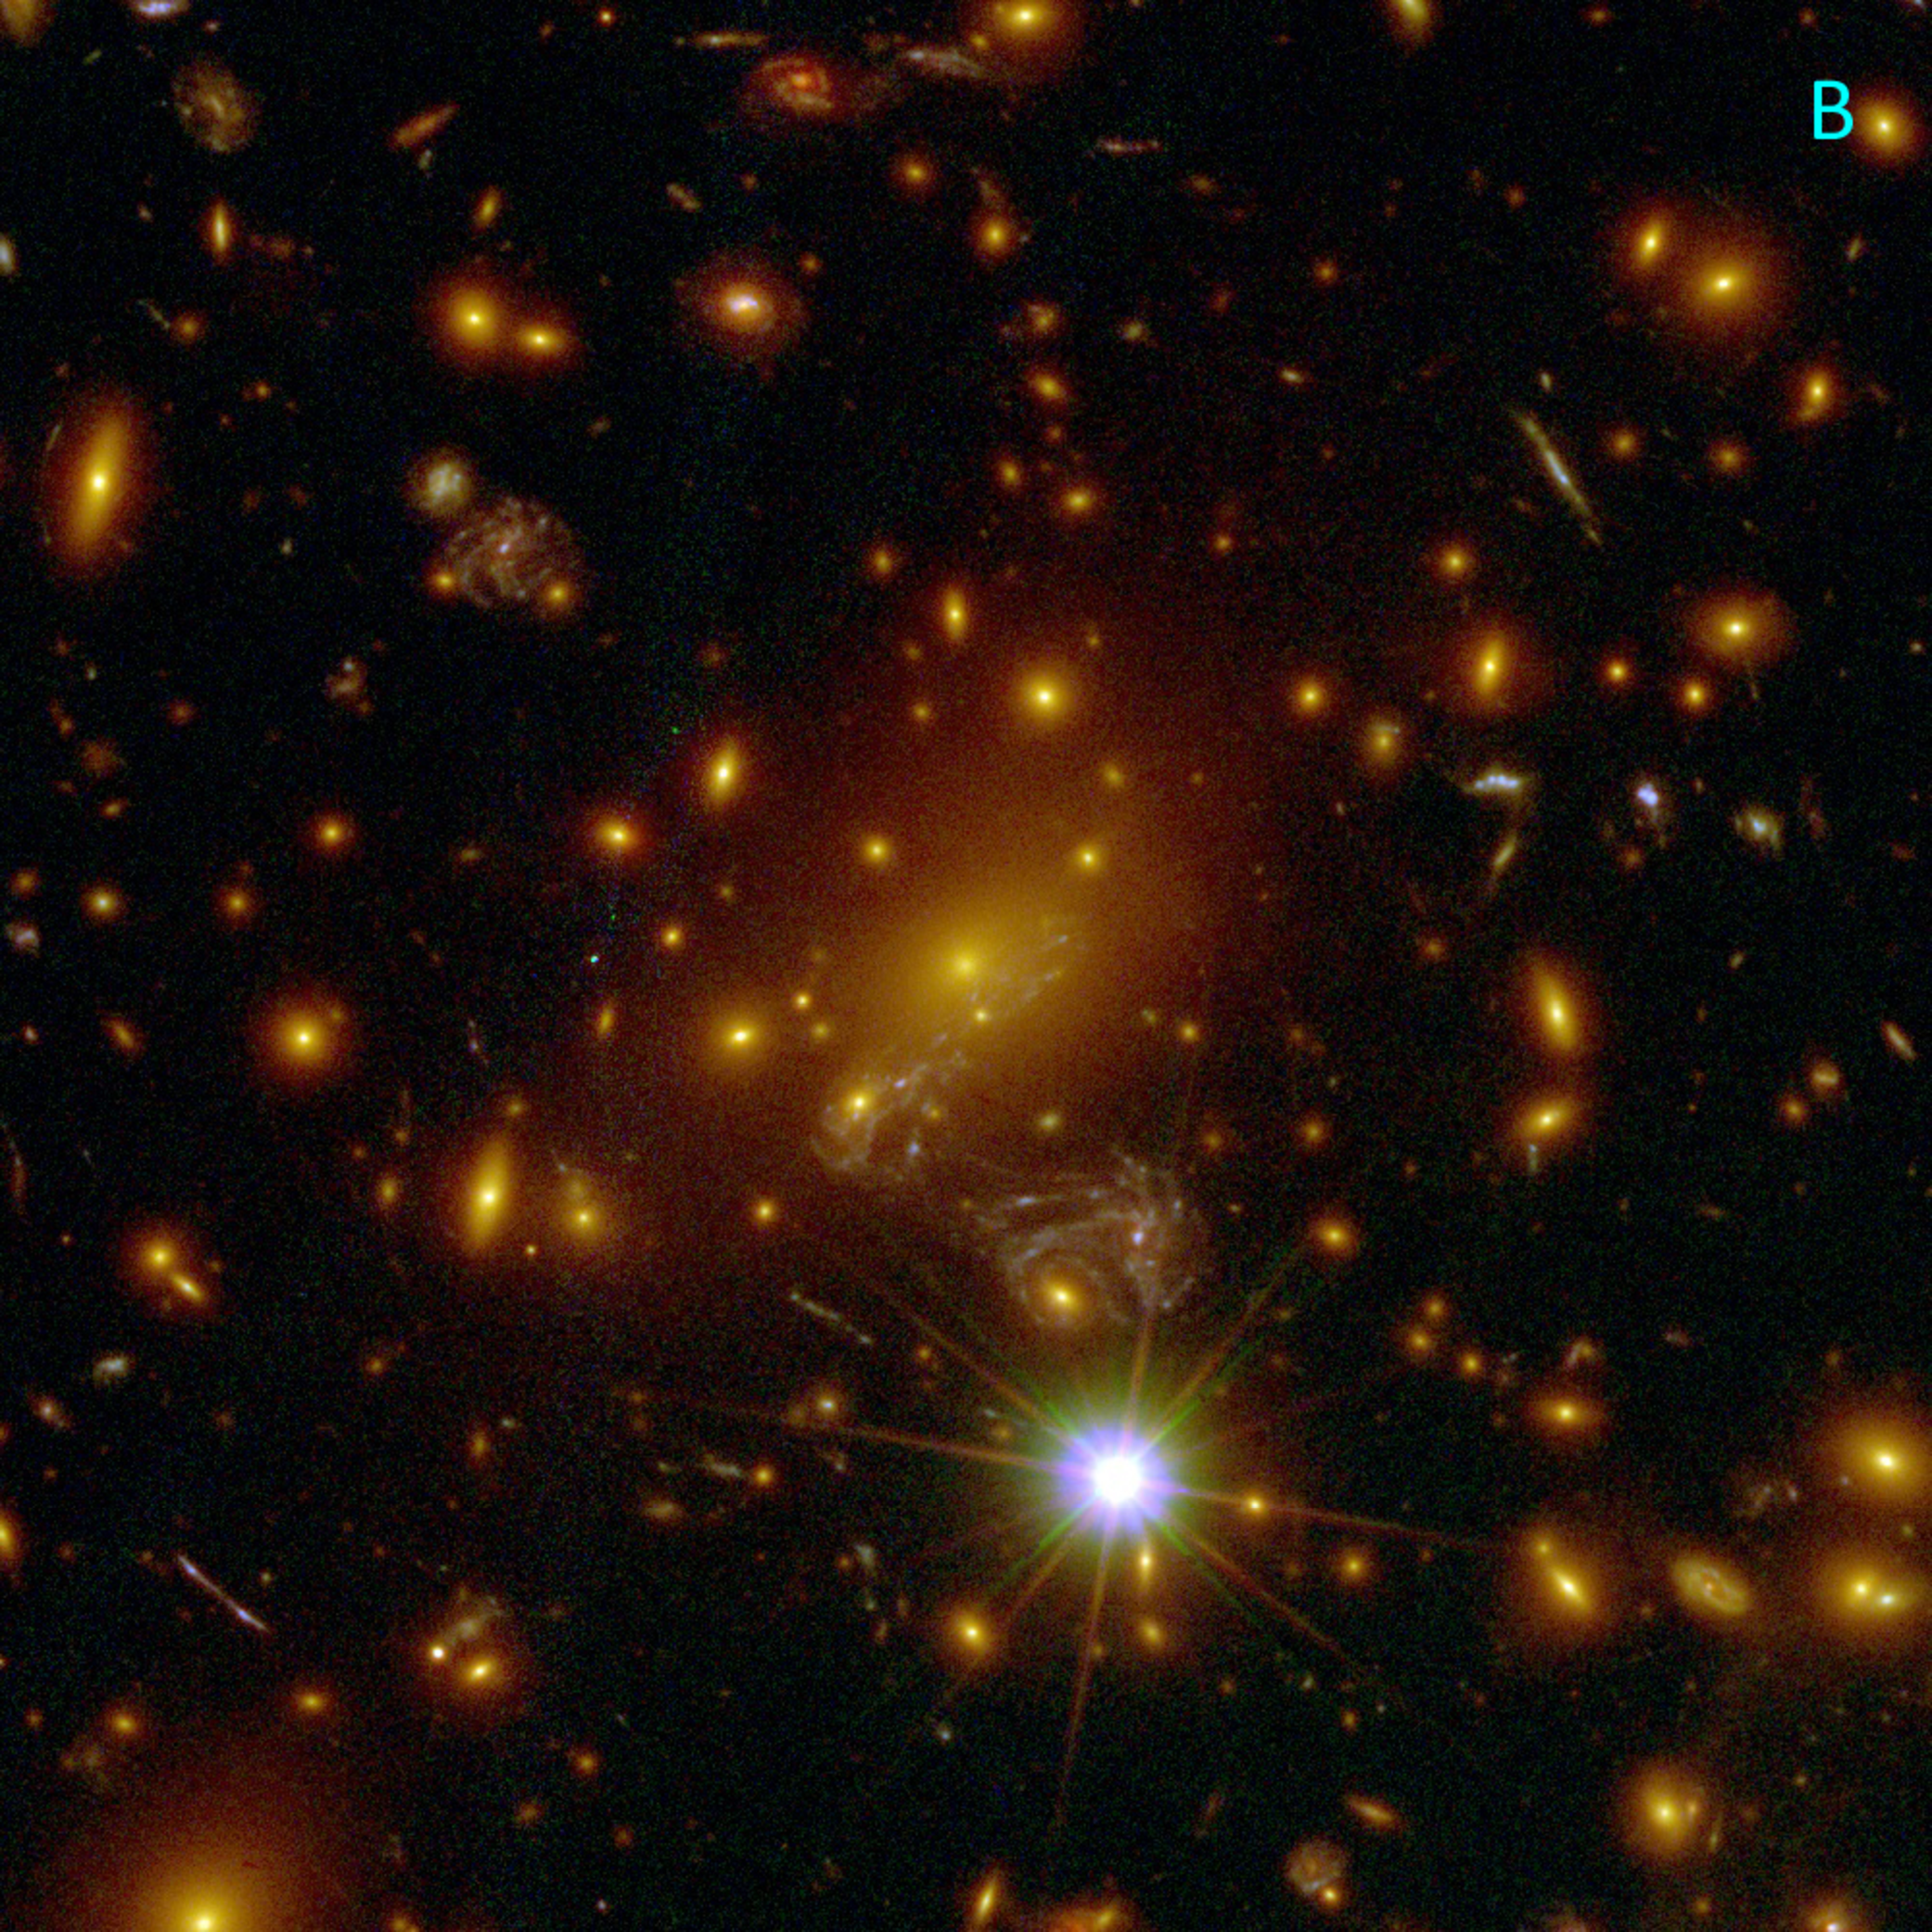
\includegraphics[width=.3\linewidth]{Figures/Chap_amas/macsj1149_opt.pdf}\hspace{10pt}
    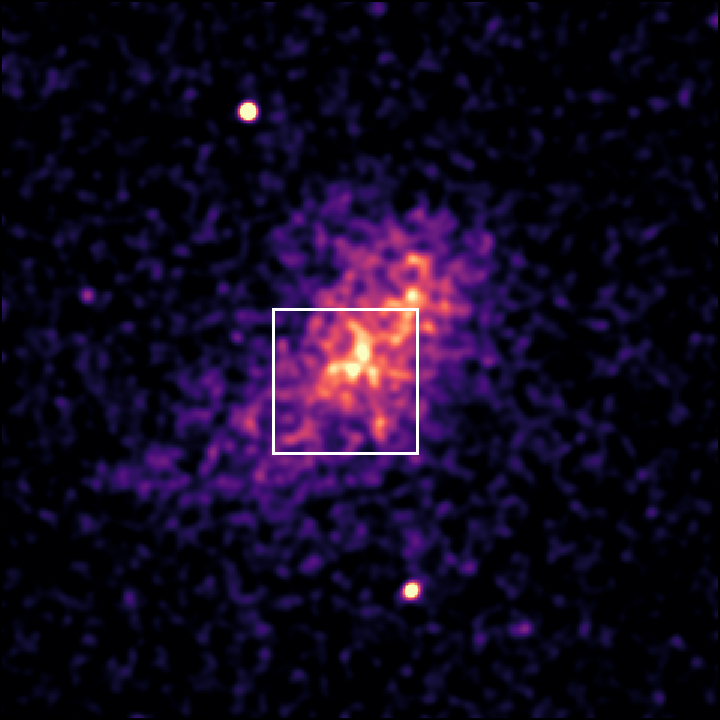
\includegraphics[width=.3\linewidth]{Figures/Chap_amas/macsj1149_X_frame.pdf}\hspace{10pt}
    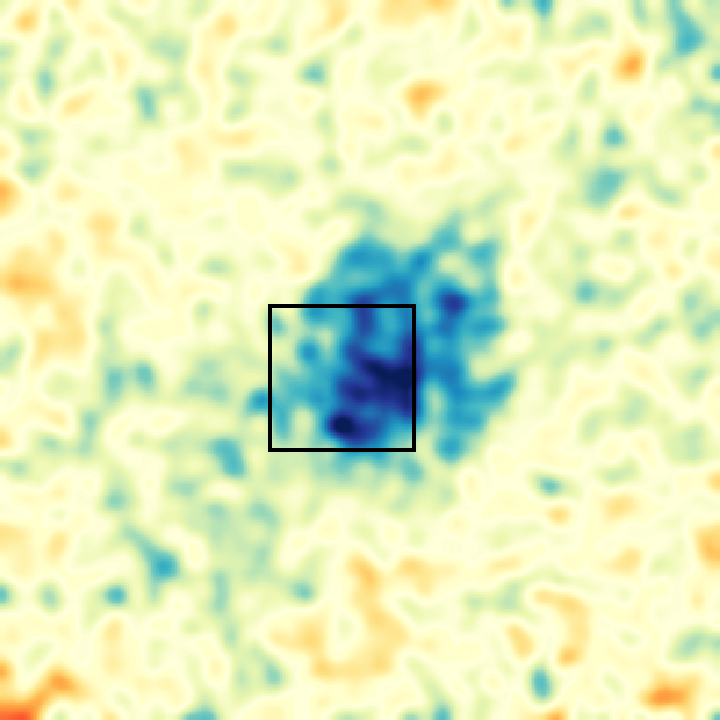
\includegraphics[width=.3\linewidth]{Figures/Chap_amas/macsj1149_SZ_frame.pdf}
    \caption{
        Cartographie de l'amas de galaxies MACSJ1149.5+2223 par le \textit{Hubble Space Telescope} en optique et infrarouge (\textit{gauche}, extraite de \cite{postman_cluster_2012}), en X avec \textit{Chandra} (\textit{centre}), et en millimétrique par l'effet Sunyaev-Zeldovich avec NIKA2 (\textit{droite}).
        La taille de la région cartographiée est de 1 arcmin pour la carte optique, et de 5 arcmin pour les cartes X et SZ.
        La région cartographiée en optique est représentée par un carré sur les cartes X et SZ.
    }
    \label{fig:macsj1149}
\end{figure*}
}

% ------------------------------------------------------------------------------------- %
\subsection{Observations en visible et infrarouge}\label{sec:opt}

De la première détection d'un amas de galaxies à la fin du 18$^\e$ siècle à l'avènement des premiers satellites X dans la deuxième moitié du 20$^\e$ siècle, les amas de galaxies étaient uniquement observés dans des longueurs d'ondes visibles \cite{biviano_messier_2000}.
L'émission visible et infrarouge des amas provient de leur composante stellaire, contenue dans les galaxies membres des amas.
Elle peut être étudiée par observations photométriques ou spectroscopiques, donnant chacune accès à des informations différentes sur les amas de galaxies observés.

Les mesures photométriques, basées sur l'acquisition d'images du ciel dans différentes bandes de longueurs d'onde, permettent l'étude des images des galaxies du champ.
La position de ces galaxies dans un diagramme couleur-magnitude permet de séparer les galaxies membres de l'amas de celles d'avant- ou arrière-plan; c'est sur ce principe que sont basés certains algorithmes de détection des amas en optique, par exemple redMaPPer \cite{rykoff_redmapper_2014}.
D'autres algorithmes existent, notamment basés sur la géométrie de la distribution de galaxies (voir par exemple \cite{adam_euclid_2019}).
La distribution des galaxies membres peut être utilisée comme un traceur du potentiel gravitationnel, offrant des contraintes sur la distribution de masse et sur l'état dynamique des amas.
En particulier, la richesse d'un amas, définie comme le nombre de galaxies membres observables, fait partie des observables étroitement liées à la masse des amas (cf. section \ref{sec:scaling}).
Elle est par conséquent fréquemment utilisée dans les relevés optiques pour estimer la masse d'amas pour lesquels des mesures individuelles de masse ne sont pas possibles\footnote{Voir par exemple \cite{costanzi_cosmological_2021,phriksee_weak_2020} pour des résultats récents.}.

L'étude des galaxies d'arrière-plan offre la possibilité de mesurer la masse d'un amas grâce au lentillage gravitationnel.
En effet, les photons en provenance de ces sources distantes sont déviés par le fort potentiel gravitationnel des amas, résultant en des distorsions de leurs images.
Ces distorsions peuvent être séparées en deux grands régimes.
Dans le cas de faibles distorsions, souvent caractérisées par une simple déformation des galaxies d'arrière-plan, on parle de lentillage gravitationnel faible (ou \textit{weak lensing}).
Celui-ci n'est souvent détectable que par étude statistique des déformations des galaxies d'arrière-plan, ne permettant pas toujours une mesure des masses individuelles des amas de galaxies (voir \cite{umetsu_clustergalaxy_2020} pour une revue sur le lentillage faible autour des amas).
Le régime de lentillage fort (ou \textit{strong lensing}) est quant à lui caractérisé par l'apparition de plusieurs images d'une même galaxie d'arrière-plan, ou bien d'une déformation extrême comme l'apparition darcs, ou plus rarement d'anneaux d'Einstein.
Il permet alors une étude plus détaillée de la distribution du potentiel gravitationnel au sein d'amas individuels.
Le lentillage gravitationnel n'est pas nécessairement présent et détectable autour d'un amas de galaxies.
En particulier, il nécessite la présence de sources d'arrière-plan, qui sont plus rares pour les amas distants, limitant le potentiel des mesures de masses par lentillage à haut redshift.
De plus, les mesures de déformations des galaxies d'arrière-plan sont fortement affectées par des effets systématiques, de par le fait qu'elles requièrent des hypothèses sur la forme réelle de ces galaxies, et qu'elles dépendent fortement des conditions d'observations et des caractéristiques des instruments utilisés (\eg\ \cite{becker_accuracy_2011,mandelbaum_instrumental_2015,grandis_calibration_2021,sommer_weak_2021}).
Ainsi, si les estimations de masses des amas ne sont pas biaisées\footnotemark, elles sont en général plus dispersées que les estimations basées sur les mesures des propriétés thermodynamiques du milieu intra-amas (\cite{pratt_galaxy_2019,umetsu_clustergalaxy_2020,grandis_calibration_2021}).
\footnotetext{Au sens où elles mesurent la masse gravitationnelle de l'amas sans reposer sur l'hypothèse de l'équilibre hydrostatique; elles sont toutefois affectées d'autres biais -- voir \eg\ \cite{pratt_galaxy_2019,grandis_calibration_2021,sommer_weak_2021}.}

Enfin, les amas de galaxies peuvent être observés aux longueurs d'onde visibles et infrarouges par spectroscopie.
Ce sont alors les spectres des galaxies qui sont mesurés, c'est-à-dire l'évolution de leur flux avec la fréquence.
De tels relevés sont capables de mesurer les redshifts des galaxies des amas, à l'aide de l'identification des longueurs d'onde observées de raies spectrales connues.
Les observations spectroscopiques d'amas de galaxies offrent aussi un moyen d'estimer la dispersion des vitesses des galaxies membres par mesure de l'effet Doppler.
Cette dispersion étant liée à la distribution de masse dans les amas, elle peut également être utilisée comme observable reliée à la masse pour des analyses cosmologiques (\eg\ \cite{munari_relation_2013, ferragamo_biases_2020}).

Plusieurs grands relevés dans les domaines visible et infrarouge sont sur le point de commencer; par exemple, le Legacy Survey of Space and Time réalisé par le Vera Rubin Observatory \cite{lsst_science_collaboration_lsst_2009} et le relevé \textit{Euclid} \cite{amendola_cosmology_2013}.
Il est prévu que ces deux relevés détectent un nombre d'amas supérieur de plusieurs ordres de grandeurs au nombre d'amas actuellement connus, avec des mesures de masses par lentillage d'une grande qualité grâce aux performances des instruments \cite{lsst_dark_energy_science_collaboration_large_2012,sartoris_next_2016}.

% ------------------------------------------------------------------------------------- %
\subsection{Observations en X}\label{sec:x}

L'un des domaines de longueur d'onde couramment utilisés pour l'étude des amas de galaxies est le domaine des rayons X.
Les amas de galaxies sont émetteurs en X principalement au travers du rayonnement de freinage (\textit{bremsstrahlung}) des électrons dans le gaz chaud du milieu intra-amas (voir \cite{bohringer_x-ray_2013} pour une revue).
La brillance de surface observée en direction d'un amas $S_X$ est liée aux propriétés thermodynamiques du milieu intra-amas:
\begin{equation}
    \label{eq:x_brightness}
    S_X = \frac{1}{4\pi (1+z)^4} \int \Lambda(T_\e, Z) \, n_\e^2 \, \d l,
\end{equation}
où $n_\e$ est la densité des électrons du milieu intra-amas, et $\Lambda(T_\e, Z)$ est la fonction de refroidissement dépendant de la température des électrons du milieu $T_\e$ et de sa métallicité $Z$, quantifiant l'abondance d'éléments plus lourds que l'hélium dans le milieu intra-amas. \\
La fonction de refroidissement peut être déterminée par étude spectroscopique du signal X, qui sera détaillée au prochain paragraphe.
L'intégration a lieu le long de la ligne de visée $l$.
Comme le montre l'équation (\ref{eq:x_brightness}), l'amplitude du signal X mesuré en direction d'un amas renseigne sur la densité d'électrons présente le long de la ligne de visée considérée.
Les observations d'amas en X permettent donc la mesure de la distribution des électrons dans le milieu intra-amas, nécessaire au calcul de la masse détaillé plus tôt (équation \ref{eq:mhse}).

En plus du continuum d'émission X due au \textit{bremsstrahlung} thermique des électrons, l'émission X dans le milieu intra-amas comporte des raies spectrales caractéristiques des transitions entre niveaux d'énergie des éléments présents dans le gaz.
Lorsqu'une observation d'un amas a permis d'accumuler suffisamment de photons X, ils est alors possible d'étudier leur distribution en énergie, qui représente le spectre du milieu intra-amas.
La connaissance de ce spectre permet de quantifier l'abondance des éléments émettant les raies spectrales étudiées, et donc la métallicité $Z$ de l'amas.
De plus, le spectre étant intimement lié à la température des électrons du gaz, les études de spectroscopie X permettent également de la mesurer\footnote{Voir \cite{bohringer_x-ray_2010} pour une revue de la spectroscopie X}.
Ainsi, des observations profondes d'amas de galaxies en X permettent de mesurer à la fois la densité et la température électronique du milieu intra-amas.
Ce milieu étant très dilué, avec des densités rarement supérieures à $10^{-2}$ électrons par centimètre cube, il peut être modélisé comme un gaz parfait.
Les mesures de densité et de pression peuvent alors être combinées pour obtenir une estimation de la pression électronique:
\begin{equation}
    \label{eq:pvnrt}
    P_\e = n_\e k_\textsc{b} T_\e,
\end{equation}
qui peut à son tour être combinée à la densité d'électrons pour calculer la masse des amas par l'équation (\ref{eq:mhse}).

Étant donnée l'opacité de l'atmosphère aux rayons X, les observations d'amas à ces longueurs d'onde ne peuvent être réalisées que depuis des satellites.
La plupart des études d'amas de galaxies en X font actuellement appel à des mesures avec les satellites \textit{XMM-Newton} \cite{jansen_xmm-newton_2001} et \textit{Chandra} \cite{weisskopf_overview_2002}.
Dans le futur, les mesures spectroscopiques fournies par la mission \textit{Athena} \cite{nandra_hot_2013} permettront la caractérisation des propriétés du milieu intra-amas avec une grande précision.
L'émission X des amas peut également être utilisée pour créer des catalogues d'amas, comme le relevé actuellement réalisé par l'instrument eROSITA \cite{merloni_erosita_2012} qui permettra la détection de plusieurs centaines de milliers d'amas.

Ainsi, l'étude du rayonnement X des amas de galaxies permet de mesurer les propriétés thermodynamiques de leur milieu intra-amas, jusqu'à leur masse, de manière autonome et sans avoir à recourir à des observations dans d'autres longueurs d'onde.
Il est toutefois à noter que l'analyse spectroscopique des photons X en provenance d'amas recquiert des observations très profondes, et est donc particulièrement coûteuse en temps.
C'est l'une des raisons qui motive la combinaison d'observations X peu profondes, ne permettant de mesurer que la distribution de densité du milieu intra-amas, avec des observations effectuées à d'autres longueurs d'onde, sensibles à d'autres propriétés physiques.
C'est par exemple le cas de l'effet Sunyaev-Zeldovich, détaillé dans la section suivante.


% ------------------------------------------------------------------------------------- %
\subsection{Observations en millimétrique: l'effet Sunyaev-Zeldovich}\label{sec:sz}

L'effet Sunyaev-Zeldovich (SZ, \cite{zeldovich_interaction_1969, sunyaev_interaction_1970,sunyaev_observations_1972,sunyaev_velocity_1980}) est une distorsion du fond diffus cosmologique due à l'interaction de ses photons avec les électrons des amas de galaxies.
L'interaction ayant lieu est une diffusion Compton inverse: les photons du CMB, peu énergétiques ($\sim 10^{-6} \;{\rm keV}$ lors de la formation des amas, à $z \lesssim 3$), diffusent sur les électrons libres du milieu intra-amas.
Ces derniers possédant une grande énergie cinétique, les photons acquièrent de l'énergie, modifiant la forme du spectre observé du CMB dans la direction des amas.

L'effet SZ peut être séparé en plusieurs composantes, parfois considérées comme des effets SZ différents, selon le processus physique à l'origine de l'énergie cinétique des électrons transmise aux photons du CMB.
Dans chacun des cas, le gain en énergie est lié aux propriétés physiques du milieu intra-amas, et l'observation des effets SZ permet de mesurer ces propriétés et donc de caractériser la physique des amas de galaxies.
Nous listons ici les trois effets SZ les plus fréquemment utilisés: l'effet SZ thermique (tSZ), cinétique (kSZ) et relativiste (rSZ).
Des revues détaillées des différents effets SZ et de leur utilisation en astrophysique et cosmologie peuvent être trouvées, par exemple, dans \cite{birkinshaw_sunyaevzeldovich_1999,carlstrom_cosmology_2002,mroczkowski_astrophysics_2019}.

\subsubsection{L'effet Sunyaev-Zeldovich thermique} % --------------------------------- %
Le milieu intra-amas est composé d'un gaz chaud ionisé, dont la température est généralement de l'ordre de $10^7 - 10^8 \;{\rm K}$.
Dans l'hypothèse d'un gaz parfait, ces températures correspondent à une énergie d'agitation thermique $3 k_\textsc{b} T / 2$ de l'ordre de $1-10 \;{\rm keV}$, bien supérieure à l'énergie des photons du CMB.
La diffusion de Compton inverse permet alors aux électrons de céder une partie de cette énergie aux photons du CMB.

La dépendance spectrale de la distorsion peut être calculée à partir de l'équation de Kompaneets \cite{kompaneets_establishment_1957, freire_oliveira_derivation_2021}: pour un bain d'électrons non-relativistes ($k_\textsc{b} T_\e \ll m_\e c^2$) traversé par des photons de fréquence réduite $x_\e \equiv h\nu/k_\textsc{b} T_\e$, on a
\begin{equation}
    \label{eq:kompaneets}
    \pdv{n}{y} = \frac{1}{x_\e^2}\pdv{}{x_\e} \left[ x_\e^4\left( \pdv{n}{x_\e} + n^2 + n \right) \right],
\end{equation}
où $n$ est l'indice d'occupation des photons, défini pour une intensité spécifique $I_\nu$ à une fréquence $\nu$ comme
\begin{equation}
    n \equiv \frac{I_\nu c^2}{2 h \nu^3},
\end{equation}
et $y$ est le paramètre de Compton, défini comme
\begin{equation}
    y \equiv \int \frac{k_\textsc{b} T_\e}{m_\e c^2} \, \d\tau_\e
\end{equation}
où $\tau_\e \equiv n_\e \sigma_\textsc{t} l$ est la profondeur optique\footnotemark\ parcourue par les photons le long de la ligne de visée $l$; $n_\e$ est la densité d'électrons, et $\sigma_\textsc{t}$ la section efficace de diffusion Thompson. \\
\footnotetext{Dans l'hypothèse d'un milieu optiquement mince.}
Cette équation peut alors aussi s'écrire
\begin{equation}
    \label{eq:sz_y}
    y = \int \frac{k_\textsc{b} T_\e}{m_\e c^2} n_\e \sigma_\textsc{t} \, \d l
      = \frac{\sigma_\textsc{t}}{m_\e c^2} \int k_\textsc{b} T_\e \, n_\e \, \d l.
\end{equation}
Dans le cas de l'effet SZ, l'énergie des photons incidents est très faible par rapport à celle des électrons, soit $x_\e \ll 1$ et donc $\partial n / \partial x_\e \gg n, n^2$.
L'équation (\ref{eq:kompaneets}) se simplifie alors, et en y injectant l'expression d'un spectre de corps noir pour les photons du CMB, on trouve l'expression de la variation d'intensité spécifique due à l'effet tSZ:
\begin{equation}
    \label{eq:sz_dI}
    \frac{\Delta I_\nu^{\rm tSZ}}{I_0} = y \times \frac{x^4 e^x}{(e^x - 1)^2} \big[ x \, {\rm coth}(x/2) - 4 \big] \big[ 1 + \delta_r(x, T) \big],
\end{equation}
où $x \equiv h\nu / k_\textsc{b}T_\textsc{cmb}$, et $\delta_r(x, T)$ traduit les corrections relativistes à l'effet tSZ, qui seront discutées par la suite, et $I_0 \equiv 2(k_\textsc{b} T_\textsc{cmb})^3 / (hc)^2$ est l'intensité spécifique du CMB.

\begin{figure*}[t]
    \centering
    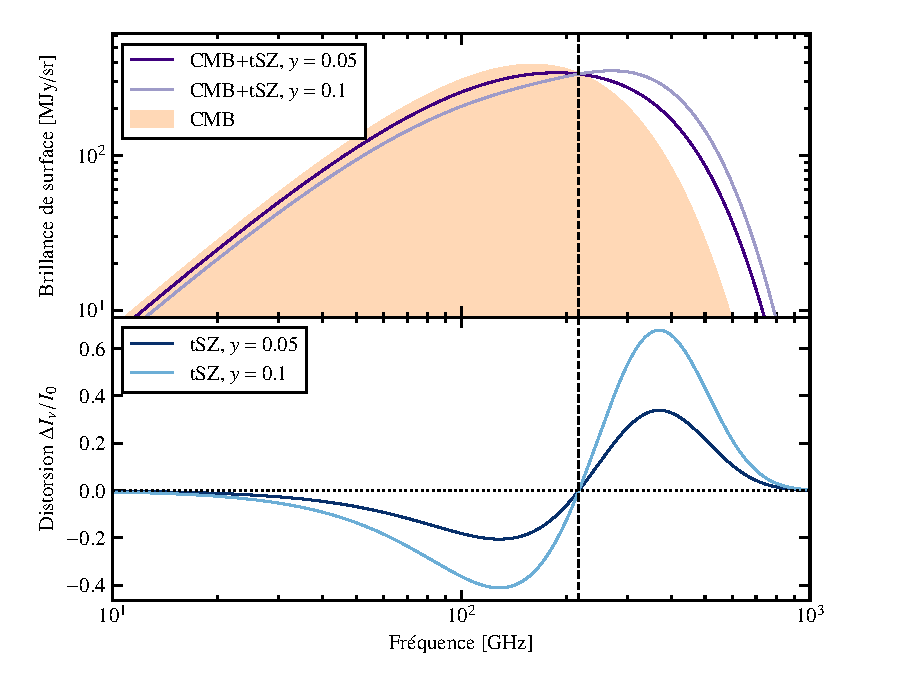
\includegraphics[width=.8\linewidth]{Figures/Chap_amas/CMB_SZ_spectrum.pdf}
    \caption{
        \textbf{Haut:} Spectre des photons du CMB (orange) et de photons ayant interagi avec un amas pour deux valeurs de paramètres de Compton $y$ (violet).
        Au premier ordre, l'effet tSZ représente un décalage du spectre vers les grandes fréquences.
        \textbf{Bas:} Distorsion spectrale due à l'effet tSZ pour les mêmes valeurs de paramètre de Compton.
        La signature observationnelle de l'effet tSZ apparaît comme un décrément dans la brillance de surface du CMB aux fréquences inférieures à 217 GHz (ligne noire verticale), et un incrément au-delà.
        Les valeurs de paramètre de Compton utilisées sont grandement exagérées pour des raisons visuelles.
        Les corrections relativistes à l'effet tSZ sont négligées.
    }
    \label{fig:tsz_spec}
\end{figure*}

La distorsion spectrale due à l'effet tSZ est représentée sur la figure \ref{fig:tsz_spec}.
On peut voir sur le panneau haut que le spectre de photons ayant interagi par effet tSZ est décalé vers les grandes fréquences, correspondant à un gain d'énergie par diffusion Compton inverse.
Le panneau bas montre la distorsion spectrale relative provoquée par l'effet tSZ (équation \ref{eq:sz_dI}).
Celle-ci se manifeste par un déficit de photons de basse énergie, et une augmentation du nombre de photons à haute énergie, par rapport au spectre du CMB avant interaction.
Ainsi, en observant le fond diffus cosmologique en direction d'amas de galaxies, on détectera un décrément dans sa brillance de surface aux fréquences inférieures à 217 GHz, et un incrément aux fréquences supérieures.
Cette signature spectrale est très caractéristique de l'effet tSZ, et permet de le différencier des autres sources astrophysiques, comme nous le verrons en \ref{sec:current_surveys}.

D'après l'équation (\ref{eq:sz_dI}), l'amplitude de la distorsion due à l'effet tSZ est donnée par le paramètre de Compton $y$.
Ce lien est également illustré en figure \ref{fig:tsz_spec}, montrant un incrément et un décrément plus importants pour des valeurs de $y$ plus élevées.
En supposant que le gaz chaud du milieu intra-amas est bien décrit par un gaz parfait (hypothèse discutée en \ref{sec:x}), l'expression du paramètre de Compton (équation \ref{eq:sz_y}) prend la forme:
\begin{equation}
    \label{}
    y(\theta) = \frac{\sigma_\textsc{t}}{m_\e c^2} \int P_\e \, \d l(\theta),
\end{equation}
où $\theta$ représente les coordonnées observées dans le ciel, et $P_\e$ est la pression due aux électrons, donnée par l'équation (\ref{eq:pvnrt}). \\
La cartographie de l'effet SZ en direction d'amas de galaxies permet donc de mesurer la distribution de pression électronique dans le milieu intra-amas.

Comme le montre l'équation (\ref{eq:sz_y}), l'amplitude de la distorsion spectrale due à l'effet tSZ ne dépend pas du redshift des amas.
Cette indépendance permet à l'effet tSZ d'être l'un des moyens privilégiés pour la détection d'amas de galaxies distants.
En effet, alors même que la brillance de surface X décroît comme $(1+z)^{-4}$ (équation \ref{eq:x_brightness}), et que les amas distants sont composés de galaxies moins brillantes, un amas de galaxies de haut redshift ne sera pas moins brillant en millimétrique qu'un amas proche de même masse.
Les relevés d'amas de galaxies par effet SZ sont donc capables de détecter des amas plus distants et donc plus anciens que leurs équivalents optiques et X.
De plus, les observations de l'effet tSZ permettent la mesure du paramètre de Compton intégré $Y$,
\begin{equation}
    \label{eq:sz_yinteg}
    Y_\Delta = 4\pi\frac{\sigma_\textsc{t}}{m_\e c^2}\int_0^{R_\Delta} P_\e(r) \, r^2 \, \d r,
\end{equation}
qui représente une mesure du contenu en énergie thermique dans le milieu intra-amas.
Ainsi, l'effet tSZ permet la détection d'amas de galaxies distants, ainsi qu'une mesure de l'énergie contenue dans leur milieu intra-amas.

\subsubsection{L'effet Sunyaev-Zeldovich cinétique} % --------------------------------- %
En plus de l'énergie provenant de leur agitation thermique, les électrons libres du milieu intra-amas peuvent posséder une énergie cinétique du fait de mouvements d'ensemble du gaz.
Une partie de cette énergie peut alors se transmettre aux photons du CMB traversant le milieu intra-amas, provoquant l'effet SZ cinétique, ou kSZ \cite{sunyaev_velocity_1980}.
Contrairement à l'effet tSZ, le mouvement des électrons ne peut par construction pas être supposé isotrope.
La distorsion spectrale du CMB s'écrit alors
\begin{equation}
    \label{eq:ksz_dI}
    \frac{\Delta I_\nu^{\rm kSZ}}{I_0} = y_{\rm kSZ} \frac{x^4 e^x}{(e^x - 1)^2}\left[ 1 + \delta_r'(x, T, v_z) \right],
\end{equation}
où $\delta_r'$ représente les corrections relativistes à l'effet kSZ, discutées par la suite, et $v_z$ est la vitesse de déplacement du gaz le long de la ligne de visée, dont dépend l'amplitude de la distorsion dans une direction $\theta$:
\begin{equation}
    \label{eq:ksz_y}
    y_{\rm kSZ}(\theta) \equiv \frac{v_z(\theta)}{c} \int \d\tau_\e
    = \frac{\sigma_\textsc{t} v_z(\theta)}{c} \int n_\e(l) \,\d l(\theta).
\end{equation}

La comparaison des équations (\ref{eq:sz_dI}) et (\ref{eq:ksz_dI}) permet de mettre en évidence la différence entre les signatures spectrales des deux effets.
Celle-ci est illustrée en figure \ref{fig:ksz_spec}, montrant que l'effet kSZ peut se manifester comme un incrément ou un décrément en brillance de surface du CMB, selon la direction du déplacement de l'amas.
En effet, d'après les équations (\ref{eq:ksz_dI}) et (\ref{eq:ksz_y}), un mouvement de gaz en direction de l'observateur ($v_z > 0$) créera un incrément en brillance de surface, et à l'inverse, le gaz s'éloignant de l'observateur ($v_z < 0$) créera un décrément.
Ainsi par exemple, dans le cas d'un amas en rotation selon un axe non parallèle à la ligne de visée, l'effet kSZ se manifestera, à une même fréquence, comme un incrément dans les régions où le gaz s'approche de l'observateur, et comme un décrément dans les régions s'en éloignant.
On remarque enfin que le maximum de la distorsion due à l'effet kSZ se situe à la fréquence à laquelle celle de l'effet tSZ est nulle, c'est-à-dire $217 \;{\rm GHz}$.
Une mesure du ciel à cette fréquence permet donc \prior\ de mesurer l'effet kSZ sans contamination par le tSZ.
Cependant, pour les amas de grande extension spatiale -- proches et massifs -- l'effet kSZ est confondu avec les anisotropies primaires du CMB, du fait de la similarité entre les spectres de puissance de ces deux types d'anisotropie.

\begin{figure*}[t]
    \centering
    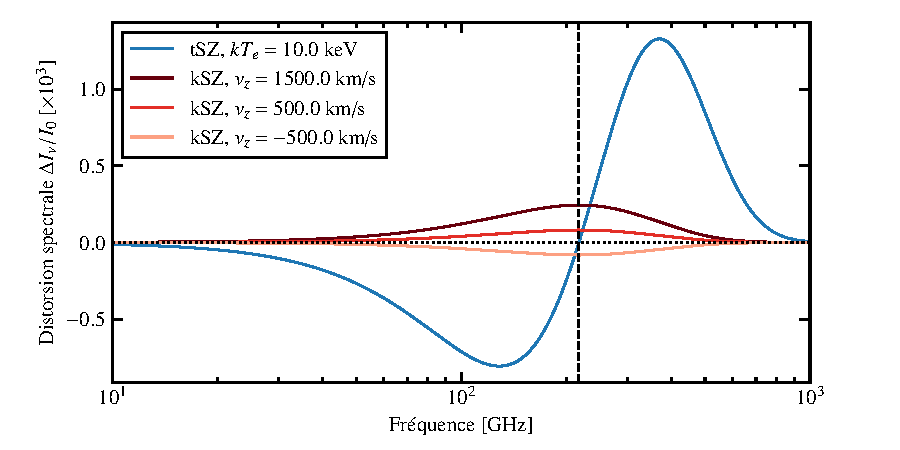
\includegraphics[width=.8\linewidth]{Figures/Chap_amas/tSZ_kSZ_spectrum.pdf}
    \caption{
        Signatures spectrales de l'effet tSZ (bleu) et kSZ (rouge) pour un amas de profondeur optique $\tau_\e = 10^{-2}$.
        L'amplitude de l'effet tSZ est calculée en supposant un milieu intra-amas isotherme avec $k_\textsc{b} T_\e = 10\;{\rm keV}$.
        Les amplitudes pour l'effet kSZ sont calculées pour différentes valeurs de vitesse le long de la ligne de visée.
        Dans les deux cas, les corrections relativistes sont négligées.
    }
    \label{fig:ksz_spec}
\end{figure*}

Comme le montre l'équation (\ref{eq:ksz_y}), la mesure de l'effet kSZ permet de mesurer le produit de la densité d'électrons et de la vitesse de déplacement du gaz.
En combinaison avec des mesures de champs de vitesses dans les amas réalisées en optique (cf. \ref{sec:opt}), l'effet kSZ offre donc l'opportunité de mesurer la densité du milieu intra-amas.
D'après l'équation (\ref{eq:mhse}), la combinaison des effets tSZ et kSZ peut donc fournir une mesure de la masse des amas dans l'hypothèse de l'équilibre hydrostatique.
Cependant, l'amplitude de l'effet kSZ est bien plus faible que celle de l'effet tSZ.
En effet, le rapport entre les deux est de l'ordre de $(k_\textsc{b} T_\e / m_\e c^2) / (v_z / c) \sim 10$ pour des vitesses de l'ordre de la centaine de km/s et des températures de l'ordre de la dizaine de keV (propriétés caractéristiques d'une grande majorité des amas de galaxies).
Cette différence d'amplitude entre les effets tSZ et kSZ pour des propriétés d'amas réalistes est visible sur la figure \ref{fig:krsz_spec}.

La mesure d'un signal kSZ significatif requiert donc une grande sensibilité, de même que des mesures à plusieurs longueurs d'onde pour pouvoir séparer sa contribution au signal total de celle de l'effet tSZ.
Des détections de l'effet kSZ existent, basées sur l'empilement de signaux en provenance de plusieurs amas (\eg\ \cite{hand_evidence_2012}) ou sur les mesures profondes d'amas dans lesquels des grandes vitesses de mouvements sont attendues (comme l'amas MACS~J0717.5+3745, \cite{mroczkowski_multi-wavelength_2012, adam_mapping_2017-1}).
Dans le cadre des observations traitées au cours de cette thèse, il est souvent négligeable: au vu du faible rapport signal sur bruit des observations, le niveau de signal kSZ sera inférieur au bruit.

\begin{figure*}[t]
    \centering
    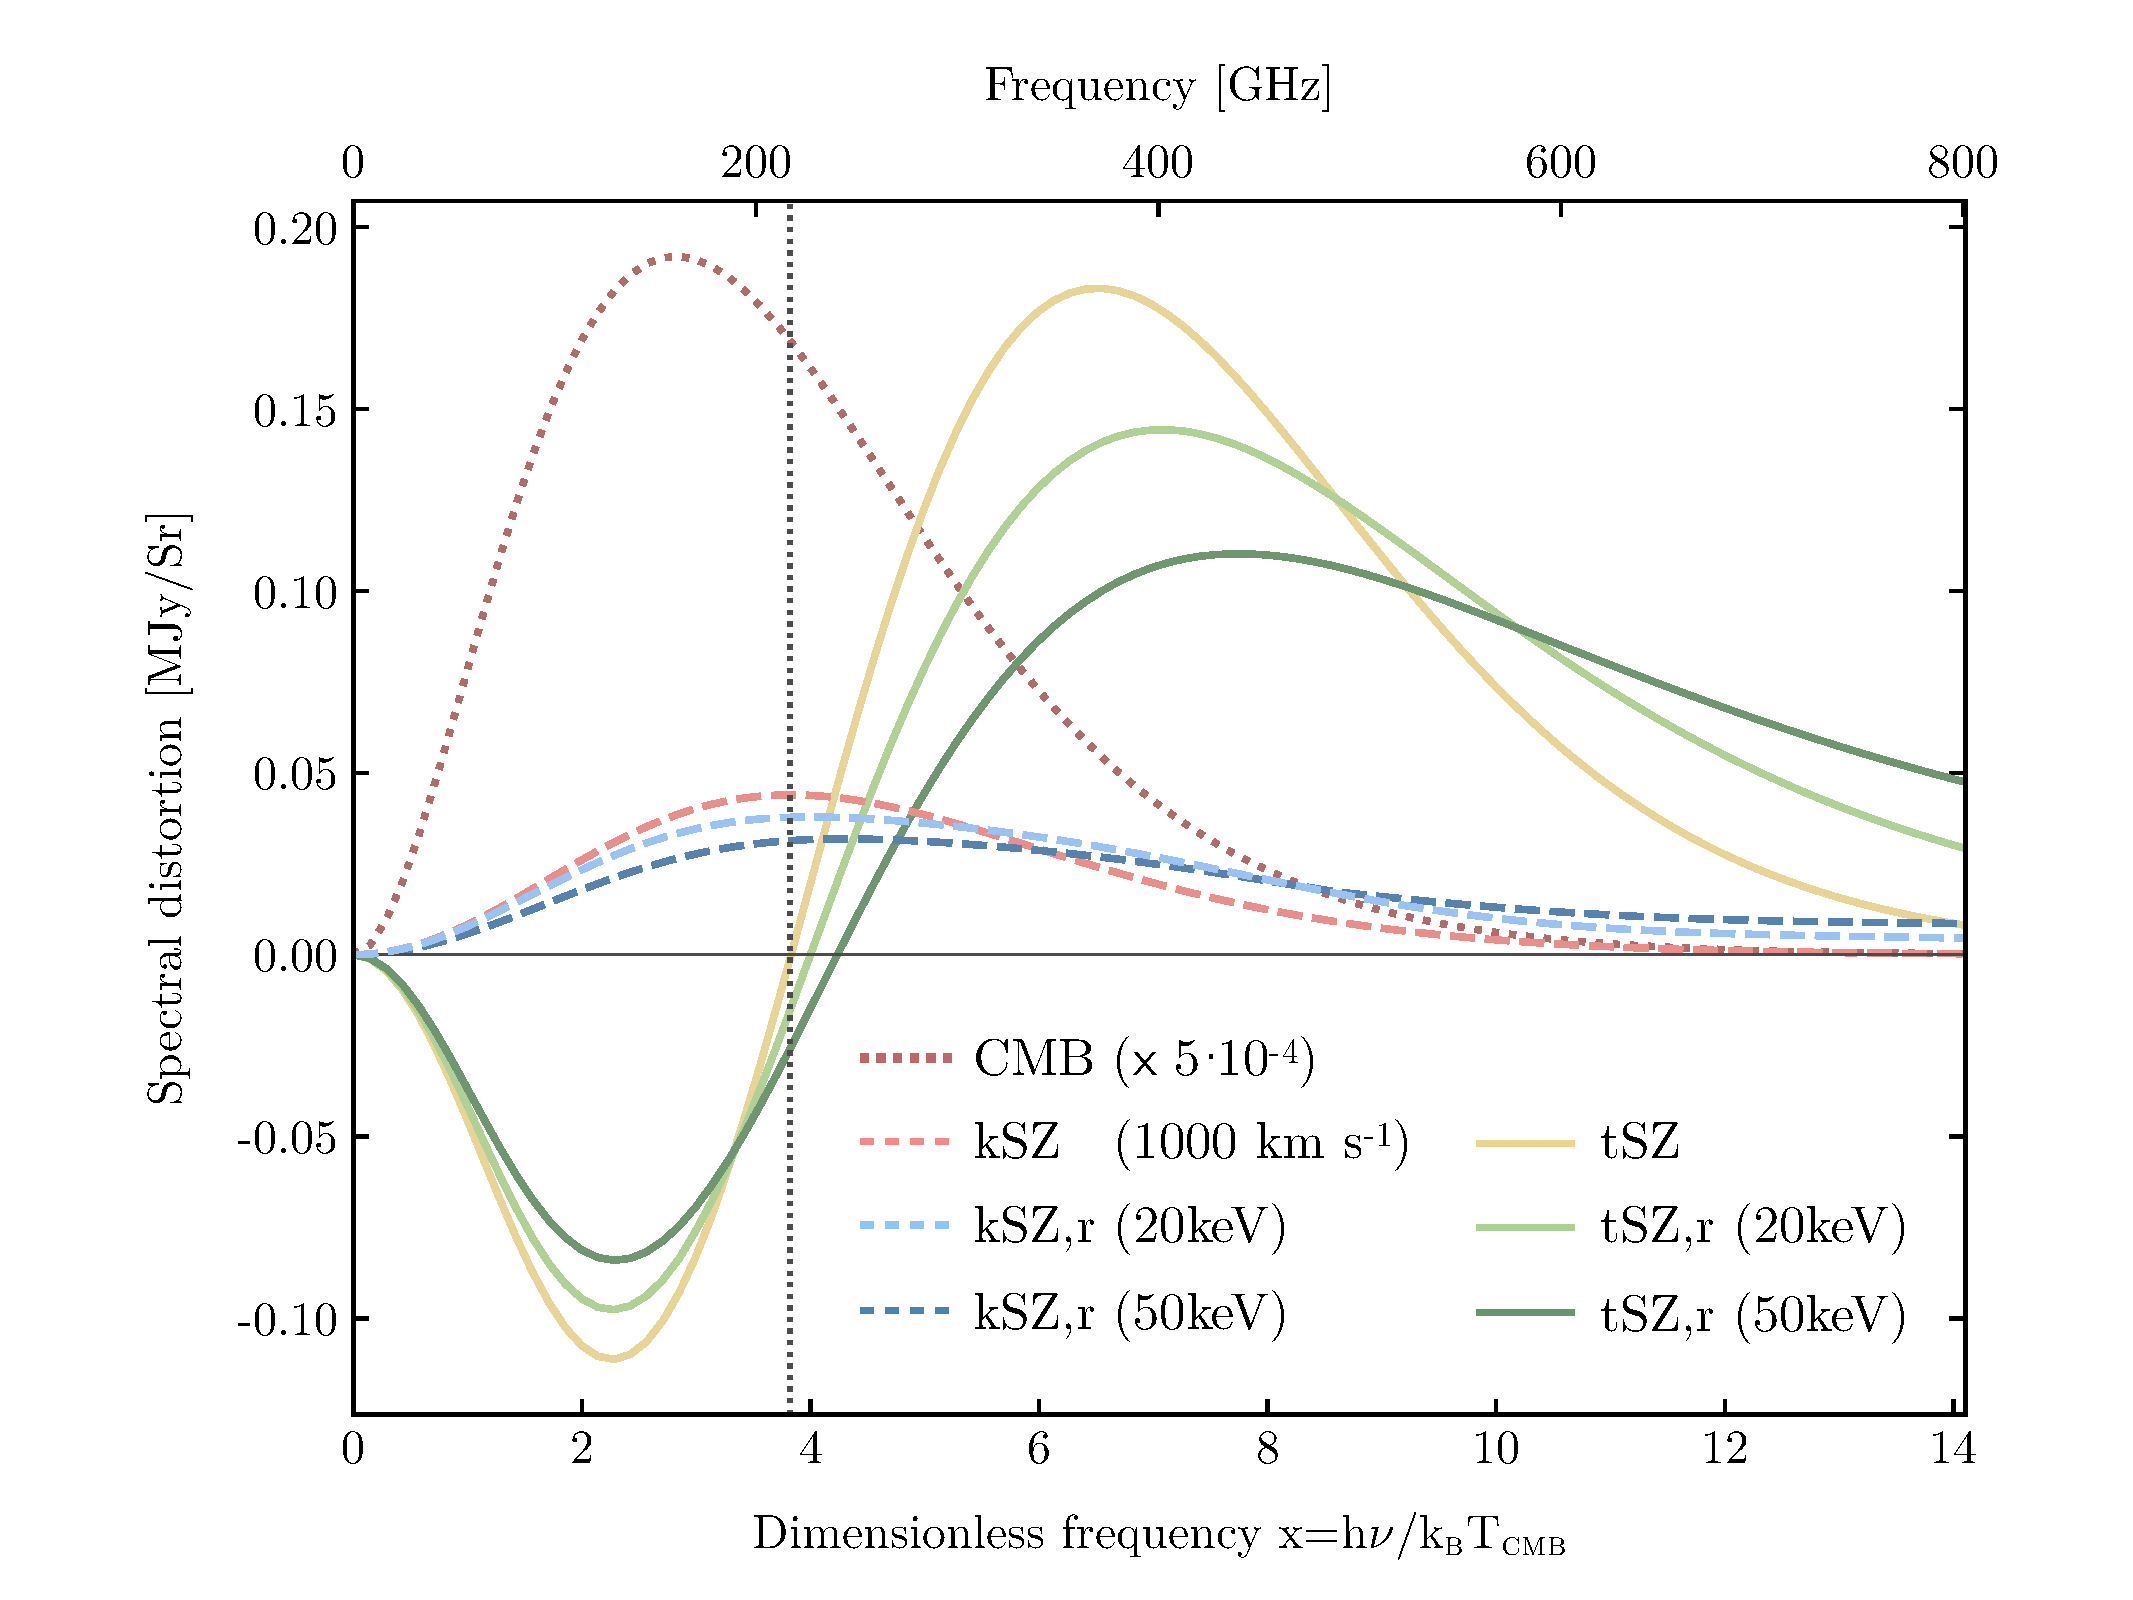
\includegraphics[width=.8\linewidth, trim={0cm 0cm 0cm 1cm}, clip]{Figures/Chap_amas/sz_tony.pdf}
    \caption{
        Spectres de l'effet tSZ (courbes pleines) et kSZ (courbes pointillées), incluant les corrections relativistes pour différentes valeurs de température.
        La profondeur optique considérée est de $\tau_\e = 10^{-2}$.
        Le spectre des photons du CMB sans interaction par effet SZ est également représenté en rouge pour comparaison.
        Figure extraite de \cite{mroczkowski_astrophysics_2019}.
    }
    \label{fig:krsz_spec}
\end{figure*}

\subsubsection{L'effet SZ relativiste} % ---------------------------------------------- %
Les corrections relativistes aux effets tSZ et kSZ, apparaissant respectivement dans les équations (\ref{eq:sz_dI}) et (\ref{eq:ksz_y}), sont parfois regroupées sous le terme d'effet SZ relativiste, ou effet rSZ.
La raison de cette dénomination est la signature spectrale particulière de ces corrections relativistes, permettant de les différencier des contributions au premier ordre des effets tSZ et kSZ, ainsi que le fait qu'elles encodent une information sur les propriétés du milieu intra-amas différentes de ces derniers.
Il est toutefois à noter qu'il s'agit bel et bien seulement de corrections relativistes aux effets susmentionnés: l'effet rSZ ne peut être détecté seul sans la présence des effets principaux.

Nous avons jusqu'à présent négligé les corrections relativistes aux effets SZ.
Cette hypothèse est facilement vérifiée dans le cas de l'effet kSZ, où les mouvements d'ensemble du milieu intra-amas ont des vitesses de l'ordre de la centaine de kilomètres par seconde, soit $\beta = v/c \sim 10^{-4}$.
Elle est moins évidente dans le cas de l'effet tSZ, où une température de $k_\textsc{b} T_\e \sim 1-10 \;{\rm keV}$ conduit à des vitesses\footnotemark $\beta = \sqrt{3 k_\textsc{b} T_\e / 2 m_\e c^2} \sim 0.1$.
\footnotetext{D'après la théorie des gaz parfaits.}

Le calcul des corrections relativistes ne sera pas détaillé ici, et nous renvoyons le lecteur vers des revues telles que \cite{mroczkowski_astrophysics_2019} pour plus de détails.
En pratique, l'effet rSZ dépend principalement de la température du milieu intra-amas, et a pour conséquence l'étalement des spectres des effets tSZ et kSZ, ainsi que le décalage de la fréquence à laquelle la distorsion due à l'effet tSZ s'annule.
Ces effets sont illustrés sur la figure \ref{fig:krsz_spec}: pour des températures croissantes, les amplitudes des spectres tSZ et kSZ sont diminuées aux fréquences inférieures à $\sim 400 \;{\rm GHz}$, et augmentées au-delà.
La fréquence correspondant au zéro de l'effet tSZ est également augmentée, de $217 \;{\rm GHz}$ en négligeant les corrections relativistes, à $\sim 240 \;{\rm GHz}$ pour une température de $k_\textsc{b} T_\e = 50 \;{\rm keV}$.
D'un point de vue observationnel, l'effet rSZ induit donc une modification des signaux tSZ et kSZ dépendant de la température du milieu intra-amas.
Cette modification peut être détectée en observant les effets SZ en provenance d'amas à un grand nombre de fréquences, afin de pouvoir séparer les contributions des termes thermique, cinétique et relativiste.
L'effet rSZ n'a à ce jour été détecté que dans des analyses sur l'empilement du signal SZ de plusieurs amas (\eg\ \cite{hurier_high_2016}), ou à travers son impact sur le spectre de puissance de la cartographie de l'effet SZ sur tout le ciel (\eg\ \cite{remazeilles_can_2019}).
Des études sont en cours pour essayer d'en obtenir des mesures individuelles, qui permettraient une première mesure de la température du milieu intra-amas aux longueurs d'ondes millimétriques, par exemple avec le spectromètre CONCERTO \cite{the_concerto_collaboration_wide_2020}.

D'autres composantes de l'effet Sunyaev-Zeldovich existent, telles que l'effet SZ polarisé ou non-thermique.
Cette thèse étudie exclusivement la composante thermique; toute mention ultérieure de l'effet SZ fera référence à l'effet tSZ, à moins que le contraire soit explicitement écrit.

% ------------------------------------------------------------------------------------- %
\subsection{Relevés d'amas de galaxies par effet SZ}

Comme nous le verrons dans la section \ref{sec:cluster_nbcount}, la contrainte des paramètres cosmologiques à l'aide d'amas de galaxies requiert la connaissance d'un catalogue d'amas de masses et redshifts connus.
De tels catalogues peuvent être construits à partir d'observations de grandes portions du ciel dans l'une des longueurs d'onde auxquelles les amas de galaxies sont détectables, puis par recensement des amas présents dans ce champ.

\subsubsection{Détection par filtre adapté} % ----------------------------------------- %
Dans le cas de l'effet SZ, la détection des amas est faite à partir de cartes dans le domaine millimétrique.
Les algorithmes de détection d'amas utilisés sont basés sur des techniques de filtre adaptés (\textit{matched filter}, voir par exemple \cite{melin_catalog_2006, melin_comparison_2012, zubeldia_understanding_2021}).
Cette approche consiste en l'exploitation d'une connaissance \prior\ de la distribution attendue du signal typique d'un amas de galaxies, et de la dépendance spectrale de l'effet étudié.
Considérons un relevé du ciel à plusieurs fréquences du domaine millimétrique $\nu_i, \, i \in [1 \dots N]$, comme le relevé réalisé à l'aide de l'instrument HFI du satellite \textit{Planck} \cite{lamarre_planck_2010,planck_collaboration_planck_2020-1}.
Les cartes peuvent être regroupées dans un vecteur $\mathbf{M}$, dont la composante $i$ représente la carte à la fréquence $\nu_i$:
\begin{equation}
    \label{eq:matched_filter}
    \mathbf{M}(\vec{x}) = y_0 \, \mathbf{S}(\vec{x}, \theta_c) + \mathbf{N}(\vec{x}),
\end{equation}
où $\vec{x}$ représente les coordonnées célestes observées, $y_0$ le paramètre de Compton central d'un amas, $\mathbf{S}(\vec{x}, \theta_c)$ la distribution spatiale du signal SZ d'un amas de taille $\theta_c$, et $\mathbf{N}(\vec{x})$ un vecteur analogue à $\mathbf{M}$ contenant les cartes de bruit aux différentes fréquences, incluant le bruit instrumental et astrophysique. \\
On définit alors un filtre adapté $\mathbf{\psi}(x, \theta_c)$, dont la transformée de Fourier s'écrit:
\begin{equation}
    \label{eq:matched_filter_filter}
    \mathbf{\psi}(\vec{k}, \theta_c) = \mathbf{\sigma}^2(\theta_c) \, \mathbf{P}^{-1}(\vec{k}) \, \mathbf{S}(\vec{k}, \theta_c),
\end{equation}
où $\mathbf{\sigma}^2(\theta_c)$ est la variance dans la carte de bruit convoluée par le filtre considéré, et $\mathbf{P}(\vec{k})$ le spectre de puissance de la carte de bruit $\mathbf{N}$. \\
La convolution des cartes formant le vecteur $\mathbf{M}$ par ce filtre permet alors d'obtenir un estimateur non-biaisé du paramètre de Compton central des amas,
\begin{equation}
    \hat{y}_0 = \int \mathbf{\psi}(\vec{x}, \theta_c) \, \mathbf{M}(\vec{x}) \, \d\vec{x}.
\end{equation}
La procédure est répétée pour plusieurs valeurs de taille de filtre $\theta_c$, afin de pouvoir détecter aussi bien des amas étendus que compacts.

Les cartes ainsi filtrées permettent d'identifier les positions des pics de paramètre de Compton, correspondant aux positions abritant des amas de galaxies.
La significativité de ces pics, donnée par les cartes du rapport $\hat{y}_0 / \sigma(\theta_c)$, permet d'associer à chaque pic la probabilité qu'il soit effectivement lié à un amas.
Ainsi, seuls les détections de significativité supérieure à un seuil fixé sont considérées comme des détections.
Le choix de ce seuil reflète la nécessité d'un compromis entre la pureté (fraction de faux positifs, détections non associées à un amas de galaxies) et la complétude (fractions d'amas existants effectivement détectés, liée au taux de faux négatifs).
En effet, plus le seuil sera bas, plus un catalogue sera complet (car incluant les amas de faible significativité), mais moins il sera pur (car composé de plus de détections ne correspondant pas à des amas).

\subsubsection{Profil de pression moyen des amas} % ----------------------------------- %
\label{sec:univ_press_prof}
Les cartes composant les vecteurs $\mathbf{M}$ et $\mathbf{N}$ dans l'équation (\ref{eq:matched_filter}) étant connues\footnotemark, l'enjeu est l'utilisation du meilleur modèle possible pour la distribution radiale du signal de l'amas, $\mathbf{S}$.
\footnotetext{Le signal SZ étant largement sous-dominant dans les relevés du ciel par rapport aux signaux contaminants (comme l'atmosphère) ou astrophysiques (comme les anisotropies primaires du CMB), les spectres de puissance des cartes de bruit $\mathbf{N}(\vec{x})$ sont en général supposés égaux à ceux des cartes complètes $\mathbf{M}(\vec{x})$.}
En effet, une mauvaise connaissance de la distribution du signal SZ en direction d'un amas entraînera de mauvaises performances pour l'algorithme de détection.

Du fait du lien entre l'amplitude de l'effet tSZ et la pression du milieu intra-amas (équation \ref{eq:sz_y}), la connaissance de la distribution radiale du signal requiert une connaissance \prior\ du profil de pression des amas\footnotemark.
\footnotetext{On note qu'il est également possible de s'affranchir de cette connaissance en utilisant un filtre adapté modélisant directement le profil de paramètre de Compton $y$, par exemple avec un smple modèle $\beta$ (approche utilisée par exemple dans les relevés réalisés à partir des données SPT, \eg\ \cite{bleem_sptpol_2020}).}
En effet, connaître la distribution de pression dans le milieu intra-amas permet d'estimer la distribution de paramètre de Compton par intégration le long de la ligne de visée, et donc la distribution de brillance de surface de l'effet tSZ.
La connaissance du profil de pression tridimensionnel moyen des amas $P(r)$ permet donc de remonter à un profil de paramètre de Compton dans le ciel $y(\vec{x})$.
Celui-ci peut alors être utilisé pour calculer le modèle de distribution spatiale de signal SZ nécessaire au calcul du filtre adapté (équation \ref{eq:matched_filter_filter}):
\begin{equation}
    \label{}
    \mathbf{S}(\vec{x}, \theta_c) = f(\nu_i) \left[ b_i \ast y(\vec{x}, \theta_c) \right],
\end{equation}
où $f(\nu)$ est la dépendance spectrale de l'effet SZ (équation \ref{eq:sz_dI}), et $b_i$ le lobe\footnotemark\ de l'instrument utilisé pour réaliser les mesures à la fréquence $\nu_i$.
\footnotetext{Le \guillemotleft lobe \guillemotright\ d'un instrument est le terme employé en radioastronomie pour désigner sa fonction d'étalement du point, ou PSF pour \textit{point spread function}.}

De plus, les cartes obtenues par convolution par le filtre adapté permettent la mesure du paramètre de Compton intégré par intégration polaire du profil de paramètre de Compton.
Par exemple, dans un rayon caractéristique $R_{500}$, on a
\begin{equation}
    \label{eq:sz_yinteg_cyl}
    Y_{500}^{\rm cyl.} = 2\pi \int_0^{\theta_{500}} \hat{y}(\theta) \theta \, \d\theta,
\end{equation}
où $\theta_{500} = c_{500} \, \theta_c$ est l'angle sous-tendu par le rayon caractéristique $R_{500}$, avec $c_{500}$ le paramètre de concentration de l'amas. \\
On note une différence fondamentale entre les grandeurs $Y_{500}$ et $Y_{500}^{\rm cyl.}$ définis dans les équations (\ref{eq:sz_yinteg}) et (\ref{eq:sz_yinteg_cyl}).
Dans la première, l'intégration réalisée est celle du profil de pression dans une sphère de rayon $R_{500}$, alors que la seconde revient à une intégration dans un cylindre de rayon $R_{500}$ et de profondeur infinie.
En pratique, la différence est faible, puisque la pression au-delà de $R_{500}$ est plusieurs ordres de grandeur plus faible qu'à l'intérieur de ce rayon.
Pour le profil de pression universel des amas de galaxies mesuré par \myciteauthor{arnaud_universal_2010} (discuté au paragraphe suivant), le rapport entre les deux est de $0.83$ (voir section 6 de \cite{arnaud_universal_2010}).
Dans la suite, nous considèrerons des valeurs calculées par intégration sphérique.

Le profil de pression moyen du milieu intra-amas est donc l'un des ingrédients nécessaires aux études cosmologiques basées sur l'effet SZ.
Dans l'hypothèse autosimilaire, la distribution radiale des propriétés thermodynamiques du milieu intra-amas doit pouvoir être bien décrite par un profil universel, mis à l'échelle par rapport à leur masse et taille caractéristique.
Les écarts à cette hypothèse proviennent de la diversité des phénomènes physiques liés aux baryons et pouvant modifier le contenu énergétique des amas.
Le profil de pression, étant directement lié au potentiel gravitationnel de l'amas par l'équation de Poisson, est supposé être le moins affecté par ces phénomènes, et particulièrement bien décrit par un profil moyen à l'échelle.
Cette hypothèse a été vérifiée expérimentalement à plusieurs reprises, menant à plusieurs mesures du profil de pression dit universel des amas de galaxies.
L'exemple le plus notable est le profil universel de \myciteauthor{arnaud_universal_2010}, mesurant le profil de pression moyen de 33 amas de galaxies à bas redshift ($z < 0.2$), en utilisant des observations X seulement.
Le profil résultant est représenté en figure \ref{fig:a10_upp}.
Cette étude montre que le profil de pression des amas est remarquablement autosimilaire: les profils des différents amas normalisés par leur masse (courbes noires en \ref{fig:a10_upp}) montrent très peu de dispersion.
Cela atteste du fait que les amas se comportent bien comme des répliques à l'échelle les uns des autres.

\begin{figure*}[t]
    \centering
    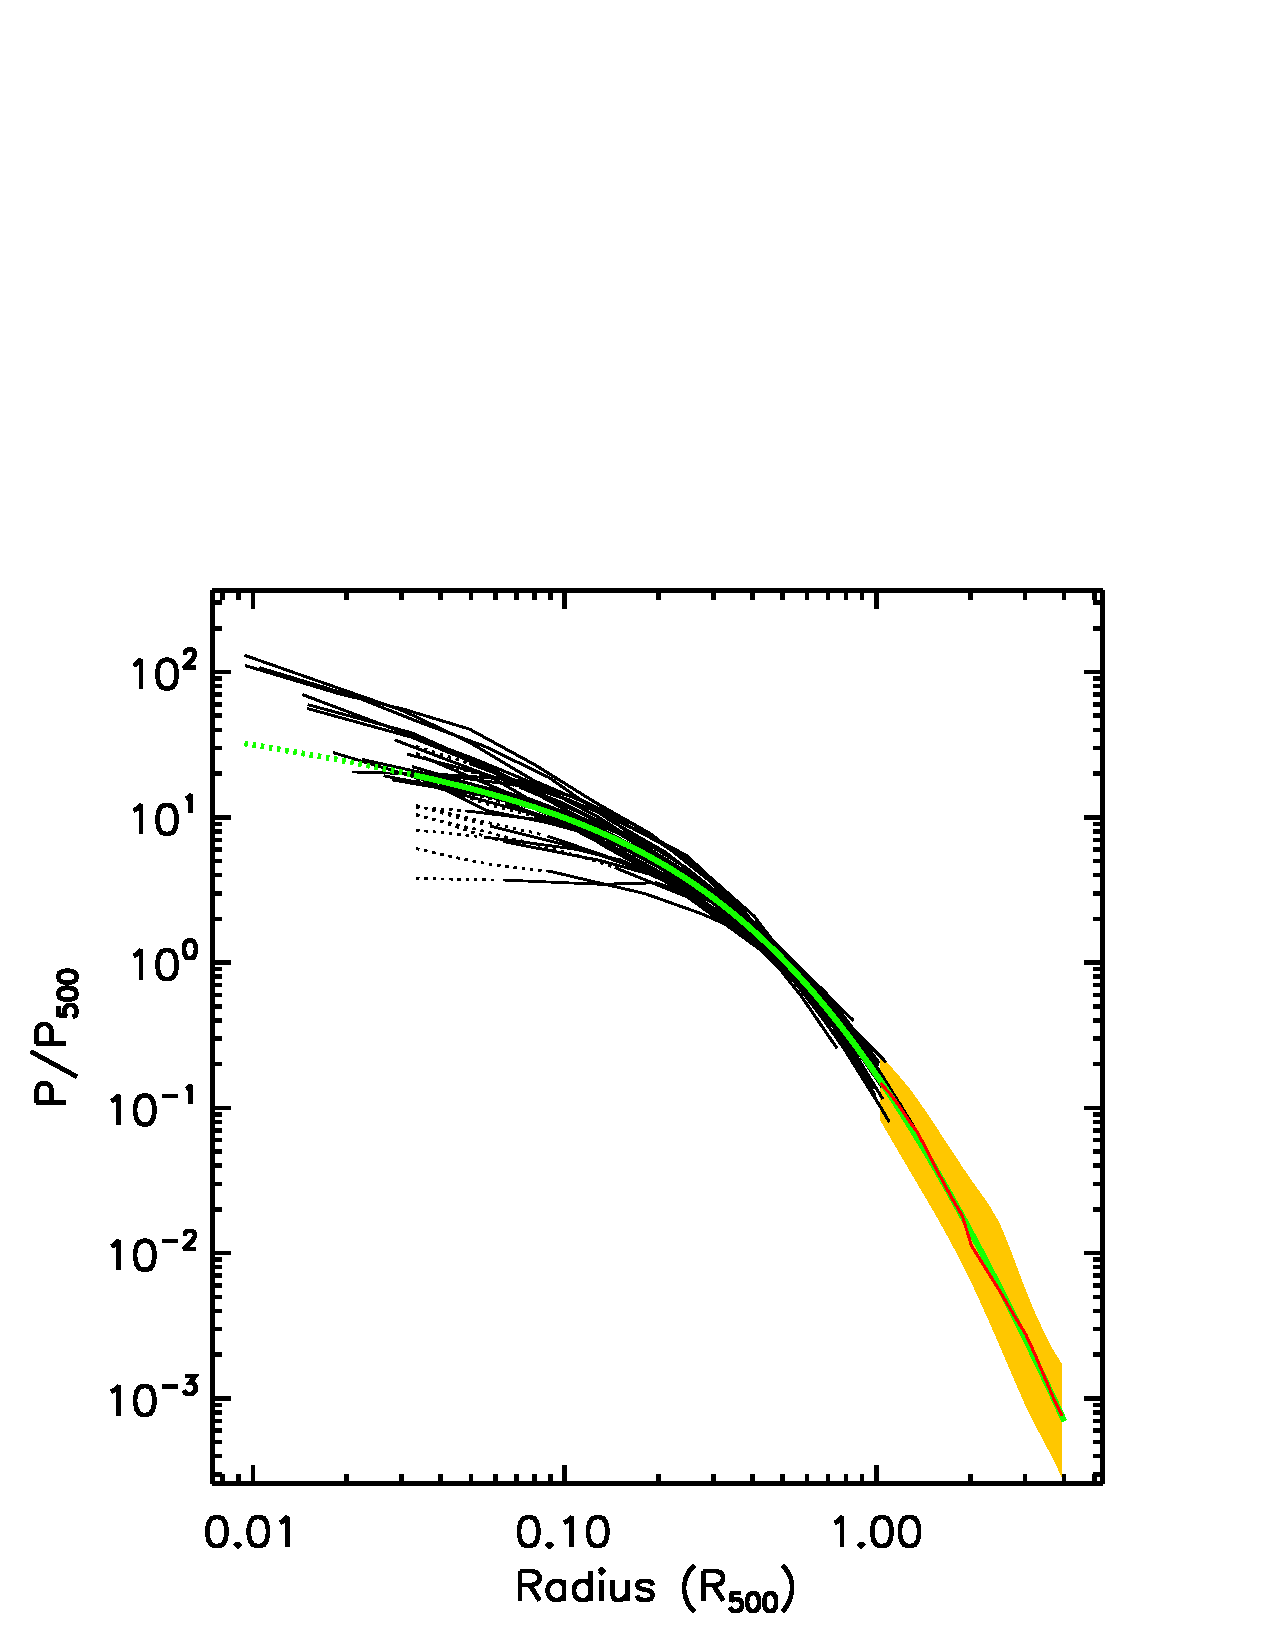
\includegraphics[width=.6\linewidth]{Figures/Chap_nk/Fig_universal.pdf}
    \caption{
        Profils de pression des amas de galaxies de l'échantillon REXCESS mesurés par \textit{XMM-Newton} (noir) et profil de pression moyen de l'échantillon, dit universel (vert).
        Figure extraite de \cite{arnaud_universal_2010}.
    }
    \label{fig:a10_upp}
\end{figure*}

% ===================================================================================== %
\section{Cosmologie par comptage d'amas de galaxies} \label{sec:cluster_nbcount}

Le lien étroit entre la formation et l'évolution des amas de galaxies et la cosmologie fait de ces derniers d'excellents outils pour la mesure des propriétés de l'Univers (voir par exemple \cite{allen_cosmological_2011} pour une revue).
Ce lien peut être exploité de plusieurs façons complémentaires, du diagramme de Hubble des amas (\eg\ \cite{kozmanyan_deriving_2019}) au spectre de puissance de l'effet SZ (\eg\ \cite{ruppin_impact_2019}), en passant par la fraction de gaz dans les amas (\eg\ \cite{mantz_cosmology_2014}).
Dans cette thèse, nous sous intéresserons au comptage d'amas de galaxies par intervalles de masse et de redshift.
Cette section présente le principe des contraintes cosmologiques par comptage d'amas.

% ------------------------------------------------------------------------------------- %
\subsection{Fonction de masse et comptage d'amas}

Comme décrit dans la section \ref{sec:cosmo_hmf}, la fonction de masse $\d N / \d M$ quantifie le nombre de halos par unité de masse dans l'Univers (équation \ref{eq:hmf}).
Afin de pouvoir l'utiliser pour prédire un nombre d'amas visibles par un observateur, il est nécessaire de tenir compte du fait que seule une portion limitée de l'Univers lui est accessible.
Deux raisons motivent ce constat.
Premièrement, l'angle solide $\Omega$ couvert par des observations doit être pris en compte, puisque les amas situés en dehors de cette région ne pourront pas être détectés.
Deuxièmement, il est nécessaire de calculer le volume effectivement accessible à un redshift donné.
Étant donné la vitesse de déplacement finie de la lumière, celle qui nous parvient depuis un amas a été émise à une époque ancienne, à un redshift d'autant plus grand que l'amas est distant.
Le volume accessible dans une tranche de redshifts $z_1 < z < z_2$ est donc celui d'une coquille sphérique, de volume
\begin{equation}
    V_c = \frac{4\pi}{3}\left[\chi^3(z_2) - \chi^3(z_1)\right],
\end{equation}
où $\chi(z)$ est la distance comobile entre l'observateur et un point de redshift $z$, qui dépend des paramètres cosmologiques. \\
On définit alors l'abondance d'amas par unités de masse, de redshift et d'angle solide potentiellement accessibles par un observateur comme:
\begin{equation}
    \label{eq:hmf_comoving}
    \frac{\d N}{\d M \, \d z \, \d\Omega} = \frac{\d N}{\d M} \frac{\d V_c}{\d z \, \d\Omega}.
\end{equation}
Enfin, la complétude du relevé traduit la probabilité de détecter un amas de galaxies à une masse $M$, un redshift $z$ et une position $\vec{r}$ donnée.
Cette probabilité est nommée \textit{fonction de sélection en masse} du relevé, $\hat{\chi}(z, M; \vec{r})$, et dépend à la fois de l'éventuelle anisotropie de la couverture du ciel réalisée, mais également de l'observable des amas considérée et de l'algorithme utilisé pour leur détection, comme discuté dans la section \ref{sec:scaling}.

Le nombre d'amas potentiellement observables entre des redshifts $z_1$ et $z_2$, entre des masses $M_1$ et $M_2$, pour un relevé de complétude $\hat{\chi}$ couvrant un angle solide $\Omega$, est alors donné par:
\begin{equation}
    \label{eq:nbcount_mass}
    n(\vec{\vartheta})
    = \int_{z_1}^{z_2} \d z
      \int_\Omega \d\Omega'
      \int_{M_1}^{M_2} \d M \,
        \hat{\chi}(z, M; \Omega') \frac{\d N}{\d M} \frac{\d V_c}{\d z \, \d\Omega'}.
\end{equation}
Celui-ci dépend des paramètres cosmologiques $\vec{\vartheta}$ au travers de la fonction de masse $\d N / \d M$ et du volume comobile $V_c$.
Ainsi, un catalogue d'amas de masses et redshifts connus peut être organisé en différentes classes $i$ de masse et redshift, et le nombre d'amas dans chaque classe $N_i$ peut être comparé à celui attendu pour un jeu de paramètres cosmologiques $\vec{\vartheta}$.
Les nombres d'amas dans chaque classe représentant un comptage discret, la comparaison se fait par le biais d'une fonction de vraisemblance poissonienne:
\begin{equation}
    \label{eq:nbcount_likelihood}
    {\rm ln}\, \mathcal{L}
    = \sum_i {\rm ln}\, P(N_i \,|\, \vec{\vartheta})
    = \sum_i \left[N_i \; {\rm ln}\, n_i(\vec{\vartheta}) - n_i(\vec{\vartheta}) - {\rm ln}\, N_i! \right].
\end{equation}
Cette fonction de vraisemblance peut être utilisée pour chercher le jeu de paramètres cosmologiques générant les comptages d'amas décrivant le mieux le jeu de données observé, ou encore injecté dans une procédure Monte Carlo à Chaînes de Markov (MCMC) pour trouver les distributions de probabilité permises pour les paramètres cosmologiques.
De telles analyses seront détaillées dans le cadre de l'analyse des propriétés thermodynamiques du milieu intra-amas, au chapitre \ref{chap:panco}.
L'exploitation cosmologique d'un relevé d'amas de galaxies requiert donc l'obtention d'un catalogue d'amas dont la masse et le redshift sont connus, qui peut être comparé à un modèle dépendant des paramètres cosmologiques à travers l'équation (\ref{eq:nbcount_likelihood}).

Un exemple d'analyse par comptage d'amas et de ses résultats est présenté en figure \ref{fig:nbcount_bocquet}, illustrant la distribution d'amas en redshift dans l'échantillon SPT-SZ $2500 \;{\rm deg^2}$ \cite{bleem_galaxy_2015} et les résultats cosmologiques issus de l'analyse \cite{bocquet_cluster_2019}.
On observe sur le panneau droit l'histogramme du nombre d'amas détectés par classes de redshift (en bleu) dans le relevé.
La région verte montre les intervalles de confiance de l'ajustement de cet histogramme par un modèle de comptage d'amas (équation \ref{eq:nbcount_mass}), en utilisant une fonction de vraisemblance similaire à l'équation (\ref{eq:nbcount_likelihood}).
Les paramètres ajustés sont (entre autres) les paramètres cosmologiques $\Omega_m$ et $\sigma_8$ d'un modèle cosmologique standard $\Lambda{\rm CDM}$.
Le panneau droit montre les intervalles de confiance obtenus sur ces deux paramètres en bleu.
Des études similaires ont pu être menées à partir des relevés réalisés par les instruments \textit{Planck} \cite{planck_collaboration_planck_2016-2} et ACT \cite{hilton_atacama_2021}.

\begin{figure*}[t]
    \centering
    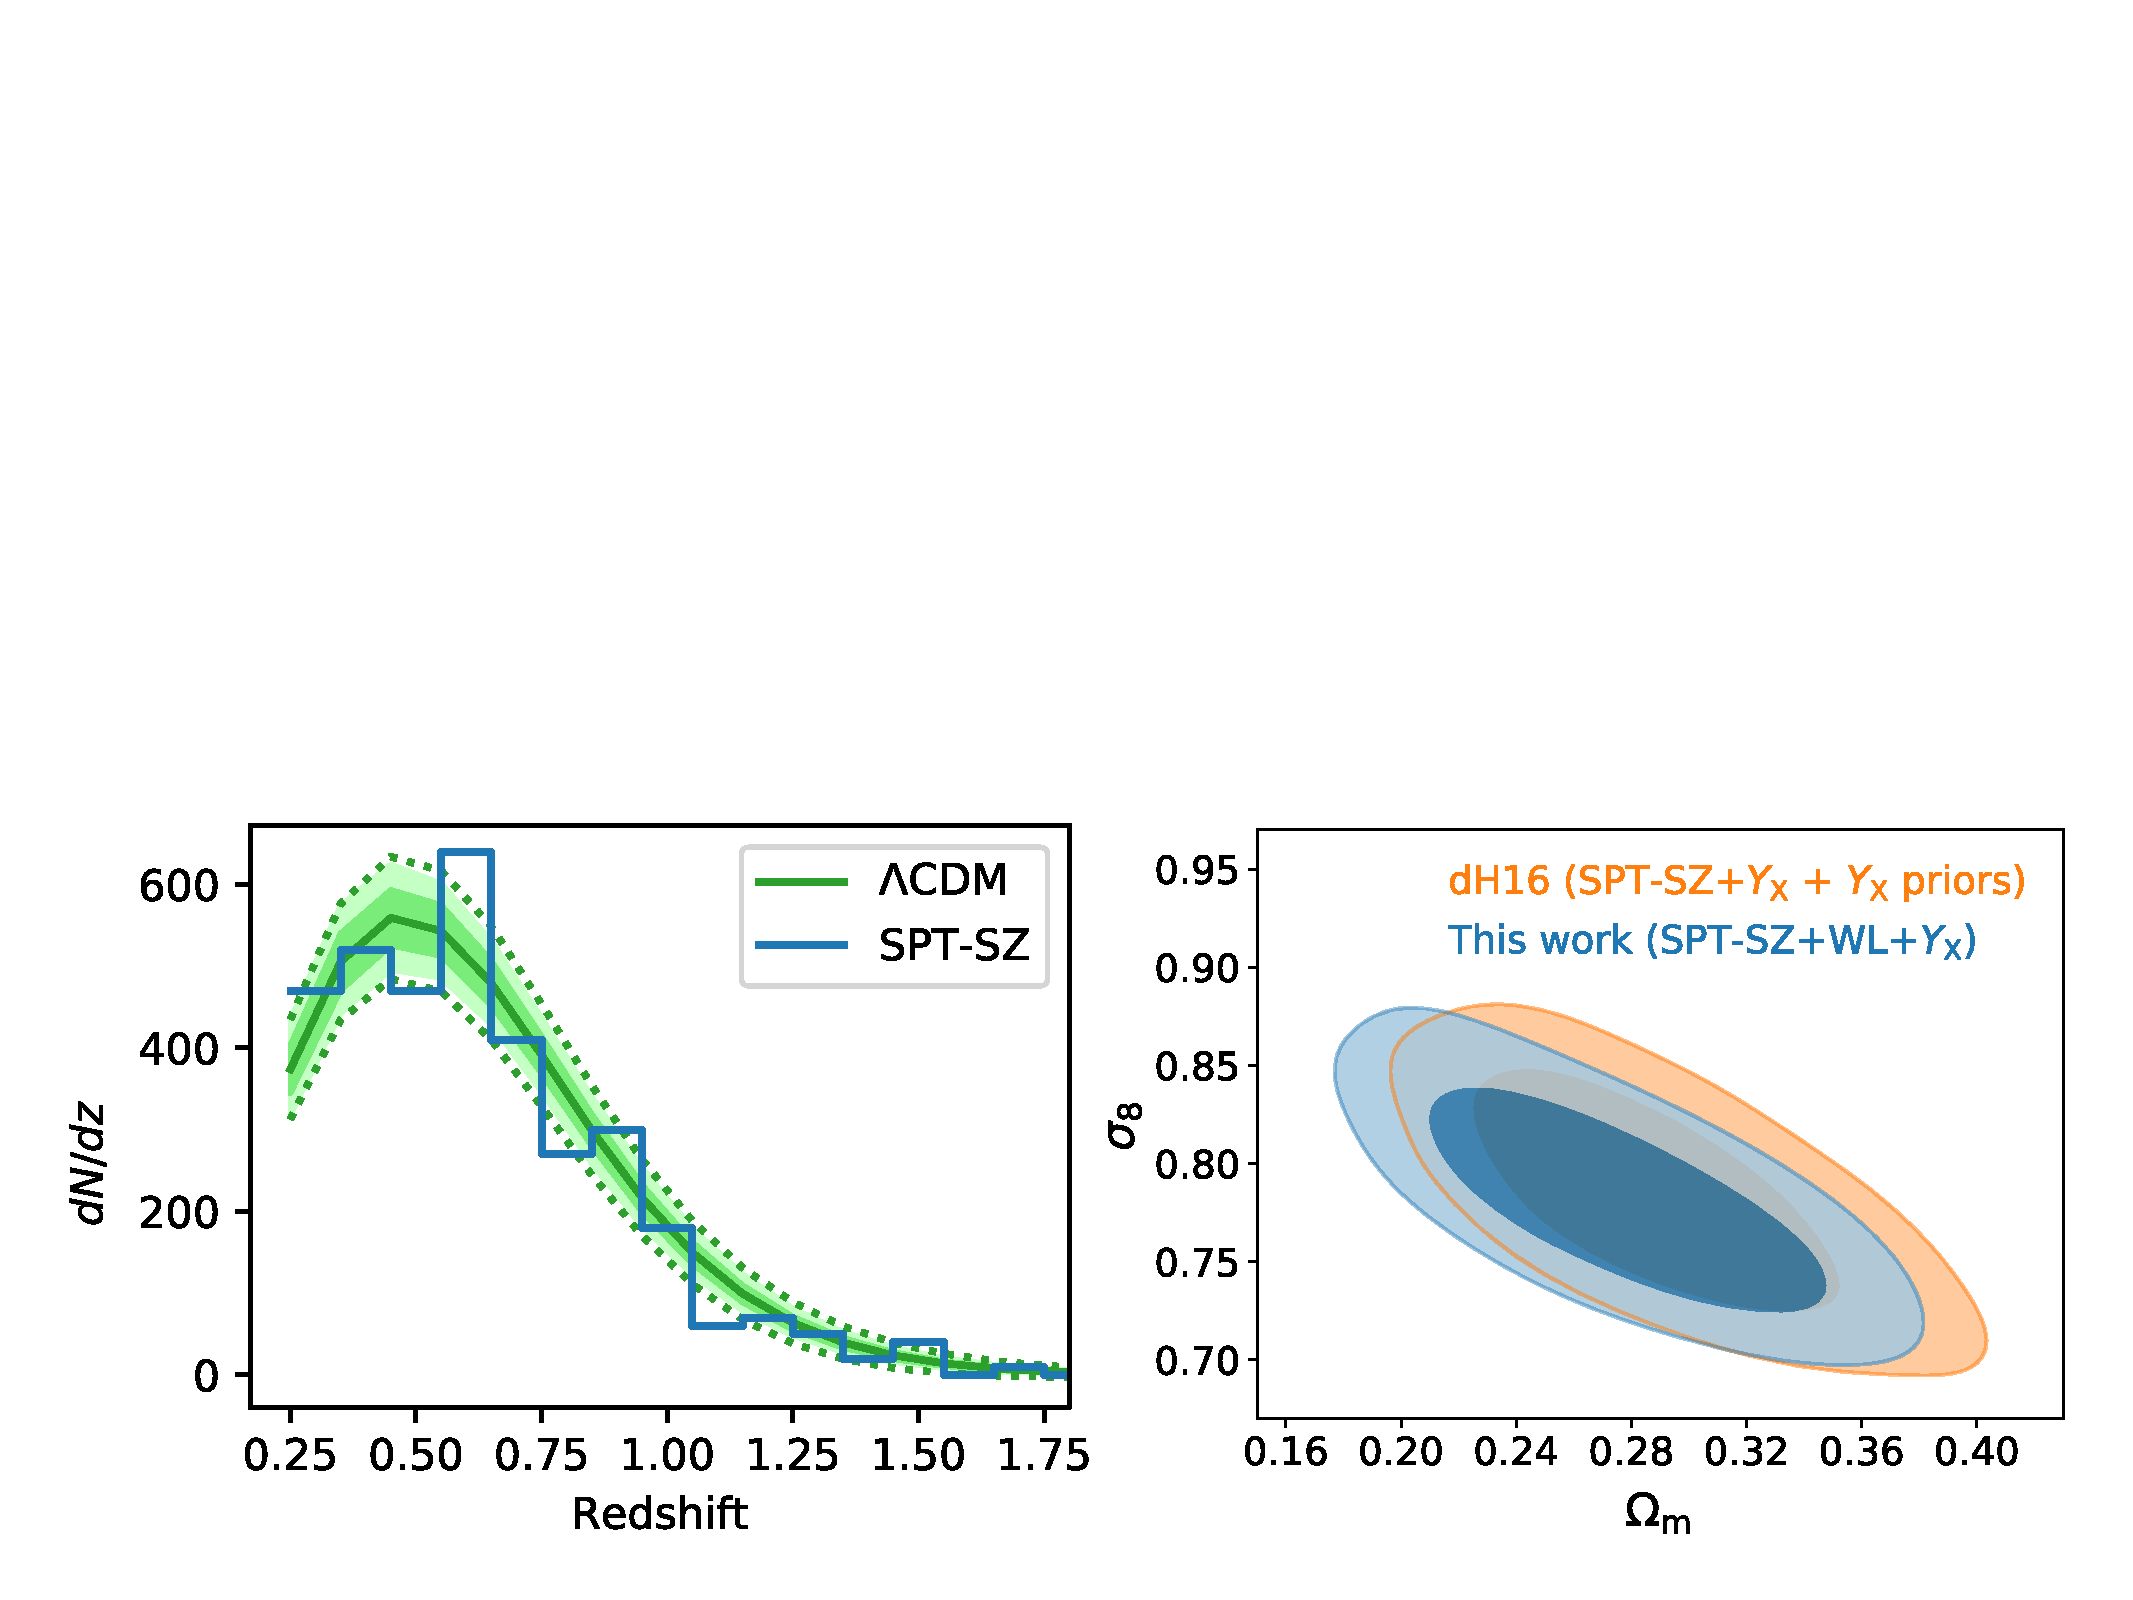
\includegraphics[width=\linewidth]{Figures/Chap_amas/bocquet.pdf}
    \caption{
        \textbf{Gauche:} Comptage d'amas par intervalles de redshift dans le relevé SPT-SZ $2500 \;{\rm deg^2}$ (bleu) et résultats de l'ajustement du modèle de l'équation (\ref{eq:nbcount_mass}) (vert).
        \textbf{Droite:} Intervalles de confiance à $1\sigma$ et $2\sigma$ obtenus sur les paramètres $(\Omega_m, \sigma_8)$ par l'ajustement représenté dans le panneau gauche (bleu).
        L'ellipse orange montre les résultats de l'étude antérieure de \cite{de_haan_cosmological_2016} pour comparaison.
        Figures adaptées de \cite{bocquet_cluster_2019}.
    }
    \label{fig:nbcount_bocquet}
\end{figure*}

% ------------------------------------------------------------------------------------- %
\subsection{Relation d'échelle masse-observable}\label{sec:scaling}

Nous avons vu dans la section précédente que les analyses cosmologiques nécessitaient l'obtention d'un catalogue d'amas de galaxies et la connaissance de leurs masses.
Il s'agit d'une contrainte forte: en pratique, peu de relevés d'amas sont en mesure d'accéder aux valeurs des masses individuelles des amas qu'ils détectent.
Il est donc nécessaire pour chaque relevé de quantifier le lien entre la masse des amas et l'une des observables directes du catalogue.
Ce lien est nommé relation d'échelle masse-observable, et sa connaissance est cruciale afin de pouvoir mener des analyses cosmologiques précises et justes.
Le chapitre \ref{chap:scaling} sera entièrement consacré à l'étude de cette relation d'échelle dans le cas de relevés SZ.
Nous nous restreindrons donc ici aux éléments essentiels pour comprendre la nécessité de telles relation pour la cosmologie avec des amas.

Les relations d'échelle fournissent donc une estimation de la masse d'un amas à partir d'une grandeur observable d'un relevé.
L'observable considérée doit donc être étroitement liée à la masse pour des contraintes précises: on qualifie alors l'observable de \textit{proxy} de masse.
Parmi les observables utilisées, on trouve la significativité de la détection des amas, c'est-à-dire la probabilité qu'une détection corresponde à un amas.
Cette grandeur est un résultat direct de beaucoup d'algorithmes de détection d'amas dans toutes les longueurs d'onde, et est fréquemment utilisée comme \textit{proxy} de masse dans les analyses cosmologiques\footnote{Par exemple dans les analyses des données SPT en SZ \cite{bocquet_cluster_2019} utilisées à titre d'exemple dans la section \ref{sec:cluster_nbcount}.}.
Plusieurs autres observables peuvent être considérées selon la longueur d'onde considérée.
En X, la luminosité et la température du milieu intra-amas sont souvent utilisées (\eg\ \cite{pacaud_xxl_2018}).
En optique, comme évoqué dans la section \ref{sec:opt}, la richesse des amas, définie par le nombre de galaxies membres, est fréquemment utilisée (\eg\ \cite{des_collaboration_dark_2020}).
En SZ, le paramètre de Compton intégré $Y_\Delta$, quantifiant le contenu en énergie thermique dans le milieu intra-amas (cf équation \ref{eq:sz_yinteg}), est fréquemment employé, pour des valeurs de contraste $\Delta$ dépendant de la couverture angulaire de l'instrument utilisé.

L'étalonnage de la relation d'échelle est effectuée en étudiant le lien entre masse des amas et observables pour un échantillon d'amas de masses connues.
Un tel échantillon peut être dressé de deux façons.
Dans le cas où un relevé offre une mesure directe de masse pour certains amas, la relation d'échelle peut être calculée à partir de ceux-ci: on parle alors d'auto-étalonnage.
Par exemple, dans un relevé optique (cf. section \ref{sec:opt}), une fraction d'amas peut avoir des masses mesurées par lentillage gravitationnel; la relation entre leur richesse et cette masse est alors calculée, et appliqué à tous les amas dont les galaxies d'arrière-plan ne permettent pas une mesure de masse (\eg\ \cite{andreon_richness-mass_2012}).
De même, les amas émettant fortement en X pourront permettre une mesure de masse par combinaison de leurs profils de densité et de température obtenu par spectroscopie (cf. section \ref{sec:x}).
Dans le cas où un relevé ne permet pas de mesure directe, une mesure de masse peut être obtenue par combinaison avec des données issues d'autres relevés, ou bien par un suivi dédié d'un échantillon d'amas.
Les bénéfices apportés par de tels suivis seront discutés en \ref{sec:follow_ups}.
Dans les deux cas, il est important que l'échantillon d'amas dont les masses sont connues soit représentatif de la population sous-jacente, afin d'éviter de biaiser les analyses par l'étude d'une population d'amas aux propriétés particulières.

Les relations d'échelle sont le plus souvent modélisées comme une relation en loi de puissance entre l'observable et la masse.
Alors, l'étude de la relation entre les logarithmes de l'observable et de la masse devient une relation affine:
\begin{equation}
    \label{eq:scaling_noproba}
    \log Y = \alpha_\ym + \beta_\ym \log M.
\end{equation}
Dans une approche probabiliste, la relation d'échelle peut être interprétée comme la probabilité pour un amas de masse $M$ d'être détecté avec une valeur d'observable $Y$.
Cette approche permet de tenir compte de la dispersion intrinsèque autour de la relation d'échelle: en effet, les différents phénomènes physiques ayant lieu au sein d'un amas peuvent affecter les observables sans modifier la masse.
En modélisant cette dispersion comme gaussienne, la relation d'échelle peut s'écrire:
\begin{equation}
    \label{eq:scaling_pdf}
    P(\log Y \,|\, \log M) = \N(\alpha_\ym + \beta_\ym \log M, \sigma_{\rm int}^2)
\end{equation}
où $\N(\mu, v)$ est la distribution de probabilité d'une loi normale de moyenne $\mu$ et de variance $v$, et $\sigma_{\rm int}$ est la dispersion intrinsèque de la relation.

L'ajustement des relations d'échelle est complexe, et peut être faire appel à un grand nombre de méthodes selon les objectifs (voir par exemple la revue de \cite{andreon_measurement_2013}).
Le chapitre \ref{chap:scaling} de cette thèse sera consacré à de tels ajustements dans le cadre d'un modèle bayésien hiérarchique.
Une fois connue, la relation d'échelle peut être injectée dans l'équation (\ref{eq:nbcount_mass}) pour exprimer cette dernière en termes d'observables plutôt que de masse.
Le nombre d'amas potentiellement observables entre des redshifts $z_1$ et $z_2$, entre des valeurs d'observable $Y_1$ et $Y_2$ est alors donné par:
\begin{equation}
    \label{eq:nbcount_obs}
    n(\vec{\vartheta}, \vec{\vartheta}')
    = \int_{z_1}^{z_2} \d z
      \int_\Omega \d\Omega'
      \int \d M \,
      \int_{Y_1}^{Y_2} \d Y \,
        \chi(z, Y; \Omega') \frac{\d N}{\d M} \frac{\d V_c}{\d z \, \d\Omega'}.
\end{equation}
où $\chi(z, Y; \Omega)$ est la \textit{fonction de sélection en observable} du relevé, liée à la fonction de sélection en masse par:
\begin{equation}
    \label{eq:nbcount_sel}
    \hat{\chi}(z, M ; \Omega) = \int P(Y \,|\, M) \chi(z, Y ; \Omega) \, \d Y.
\end{equation}

Le nombre d'amas attendu dépend donc à la fois des paramètres cosmologiques $\vec{\vartheta}$ et des paramètres de la relation d'échelle, $\vec{\vartheta}'$.
La connaissance des valeurs des paramètres $\vec{\vartheta}' = (\alpha_\ym, \beta_\ym, \sigma_{\rm int})$ décrivant le mieux les données est alors insuffisante, puisqu'elle ne permet pas de propager l'incertitude sur ces grandeurs au calcul des paramètres cosmologiques.
Il est donc nécessaire de connaître les distributions de probabilité des paramètres de la relation d'échelle.
Ces distributions peuvent être obtenues par l'ajustement de la relation par MCMC, qui sera discuté dans le chapitre \ref{chap:scaling}, et utilisées comme \prior\ sur les paramètres dans l'ajustement simultané des paramètres cosmologiques et de ceux de la relation d'échelle.
De telles études permettent de tenir compte des effets systématiques associés à l'étalonnage de masse des amas de galaxies dans les analyses cosmologiques (par exemple en SZ \cite{bocquet_cluster_2019} ou en optique \cite{des_collaboration_dark_2020}).

% ===================================================================================== %
\section{État de l'art et perspectives}

% ------------------------------------------------------------------------------------- %
\subsection{Relevés d'amas et résultats cosmologiques actuels}\label{sec:current_surveys}

Le comptage d'amas de galaxies s'est imposé comme l'une des sondes cosmologiques majeures des dernières années grâce à l'augmentation du nombre d'amas détectés dans les relevés réalisés aux différentes longueurs d'onde discutées en \ref{sec:cluster_obs}.

En optique, les relevés du Sloan Digital Sky Survey (SDSS, \cite{rykoff_redmapper_2014,costanzi_methods_2019}), et plus récemment des Dark Energy Survey (DES, \cite{des_collaboration_dark_2020}) et Kilo-Degree Survey (KiDS, \cite{lesci_amico_2020}), ont permis de construire des catalogues de plusieurs milliers d'amas de galaxies, jusqu'à des redshifts d'environ 0.6.
Ces relevés ont utilisé les mesures de lentillage faible pour l'auto-étalonnage des masses des amas de ces catalogues (voir section \ref{sec:scaling}).

Les catalogues d'amas de galaxies dressés grâce aux différents relevés réalisés par le satellite \textit{ROSAT} (\eg\ RASS \cite{bohringer_northern_2000} ou REFLEX \cite{bohringer_rosat-eso_2004}) ont laissé un héritage conséquent pour l'étude des propriétés des amas de galaxies en X, en particulier de leurs propriétés thermodynamiques et des relations d'échelles liant brillance de surface X et masse d'amas (\eg\ \cite{arnaud_universal_2010, pratt_galaxy_2009,pratt_gas_2010}).
Récemment, les relevés d'amas en X ont consisté en plusieurs relevés profonds concentrés sur de petites régions du ciel.
En particulier, le relevé XXL a permis de construire un catalogue de 356 amas dans une région de $50 \;{\rm deg^2}$ jusqu'à des redshifts d'environ 1 \cite{adami_xxl_2018}.

Les différents relevés du CMB réalisés au cours de la dernière décennie ont permis la construction de grands catalogues d'amas grâce à l'effet SZ, notamment avec le satellite \textit{Planck} \cite{planck_collaboration_planck_2016-1}, le South Pole Telescope (SPT, \cite{bleem_sptpol_2020}) et l'Atacama Cosmology Telescope (ACT, \cite{hilton_atacama_2021}).
Ce dernier constitue l'un des relevés d'amas de galaxies les plus grands et profonds existant à la date de l'écriture de cette thèse, avec plus de 4000 amas jusquà des redshifts d'environ 1.9 \cite{hilton_atacama_2021}.

La distribution en masse et redshift des catalogues d'amas obtenus par l'effet SZ est représentée en figure \ref{fig:cluster_catalogs_mz}.
Celle-ci suit la forme du produit de la fonction de masse et du volume comobile, qui fournit une prédiction du nombre d'amas de masse et redshift donné accessible par un observateur\footnotemark.
\footnotetext{Comme expliqué dans la section \mypageref{sec:cluster_nbcount} (équation \ref{eq:hmf_comoving}).}
On voit que la plupart des amas détectés par ces relevés se situent à des redshifts inférieurs à 1.5, et à des masses supérieures à $2 \times 10^{14} \;M_\odot$.
On y observe également les couvertures en masse et redshift de chacun des relevés.
Le relevé réalisé avec le satellite \textit{Planck} est caractérisé par une moins grande résolution angulaire que ses contreparties au sol, due à la difficulté technique liée à l'envoi d'un télescope aussi large que le SPT (10 m) ou l'ACT (6 m) dans l'espace.
Par conséquent, il est sensible à de plus grandes échelles angulaires, ce qui le rend plus complet à bas redshift et haute masse, mais moins à haut redshift et faible masse.
La profondeur du relevé influe également sur la possibilité de détecter des amas.
Ainsi, les relevés ACT et SPT, plus profonds que le relevé \textit{Planck}, sont plus complets pour les amas peu lumineux (de basse masse) que ce dernier.
Enfin, le nombre d'amas détectés par un relevé dépend évidemment de sa couverture angulaire.
Le relevé \textit{Planck} couvre tout le ciel ($\sim 41\,000 \;\unit{deg^2}$), alors que les relevés ACT et SPT ne couvrent respectivement qu'un tiers et un huitième de cette surface.
En conclusion, le catalogue d'amas issu du relevé \textit{Planck} fournit une vision très complète de la distribution d'amas massifs et proches existant dans l'Univers observable, alors que les relevés ACT et SPT offrent une meilleure couverture de la distribution d'amas distants et peu massifs sur une portion plus restreinte du ciel.

\begin{figure*}[t]
    \centering
    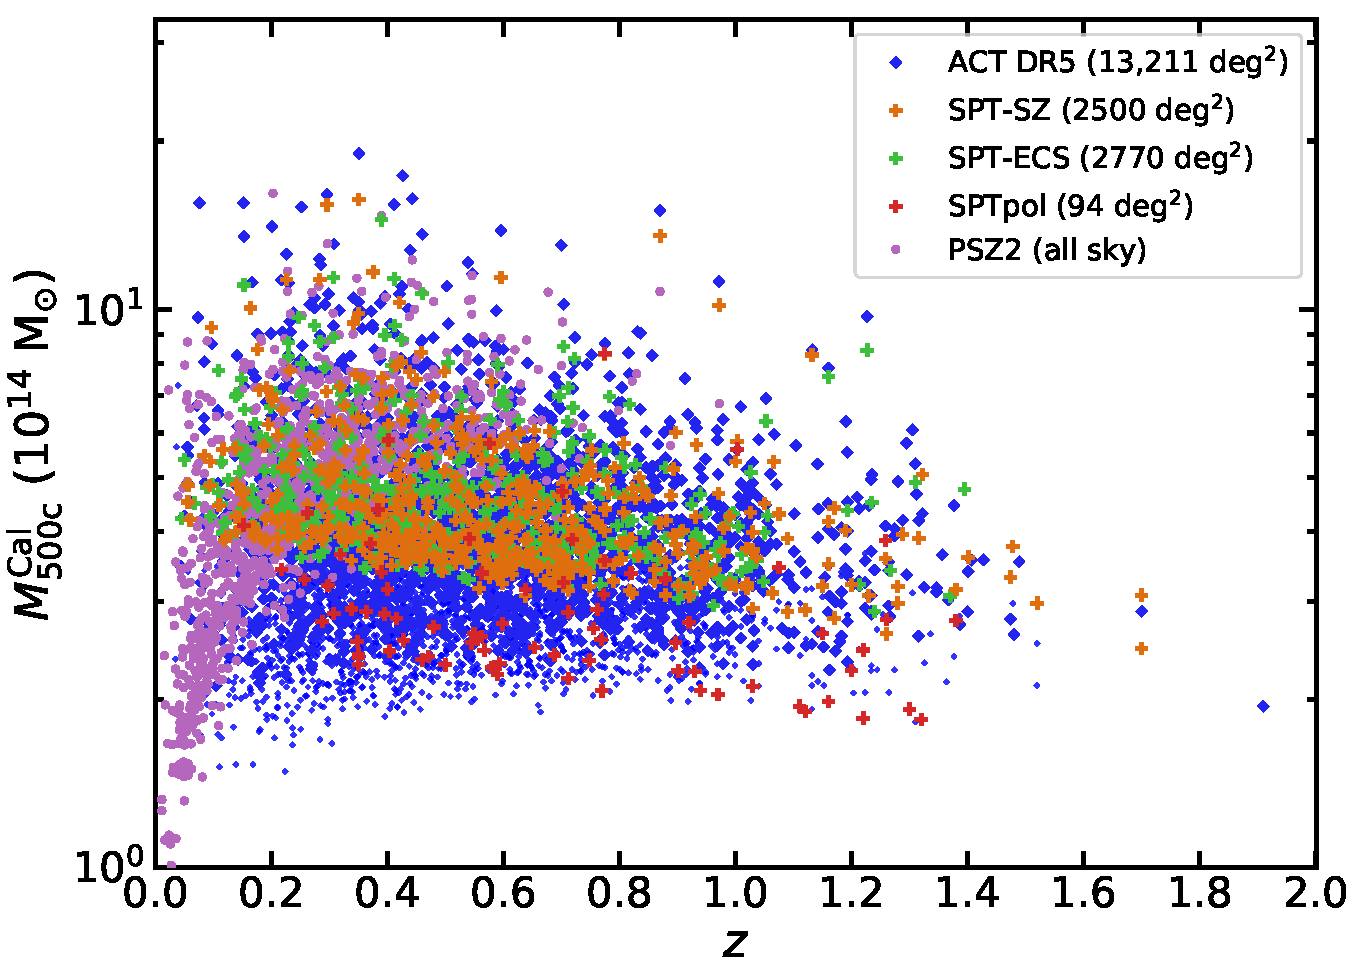
\includegraphics[width=.6\textwidth]{Figures/Chap_amas/mz_sz.pdf}
    \caption{
        Distribution dans le plan masse-redshift des amas détectés par les relevés ACT (bleu, \cite{hilton_atacama_2021}), SPT (orange \cite{bleem_galaxy_2015}, vert \cite{bleem_sptpol_2020} et rouge \cite{huang_galaxy_2020}) et \textit{Planck} (violet, \cite{planck_collaboration_planck_2016-1}).
        Figure extraite de \cite{hilton_atacama_2021}.
    }
    \label{fig:cluster_catalogs_mz}
\end{figure*}

Ces catalogues ont pu être utilisés pour contraindre les paramètres cosmologiques grâce à la distribution des amas en masse et en redshift.
La figure \ref{fig:cluster_S8} montre les contraintes apportées par chacun de ces relevés sur la combinaison de paramètres $S_8 \equiv \sigma_8 \sqrt{\Omega_m/0.3}$, discutée en section \mypageref{sec:cosmo_hmf}.
Les mesures de ce paramètre par des analyses des anisotropies primaires du CMB et de la distribution des galaxies sont également présentées à titre de comparaison.
Si les résultats apparaissent globalement en accord, à l'exception du comptage d'amas dans le Dark Energy Survey \cite{des_collaboration_dark_2020}, les sondes basées sur l'Univers récent semblent favoriser des valeurs plus basses de $S_8$ que le CMB.

Ce constat, en parallèle avec la tension entre le CMB et les autres sondes dans les mesures du taux d'expansion de l'Univers (\eg\ \cite{riess_large_2019,wong_h0licow_2020,efstathiou_h0_2021}), souligne la nécessité de l'étude des effets systématiques affectant l'inférence des paramètres cosmologiques.
En effet, si une différence dans la mesure des paramètres cosmologiques par des sondes différentes peut être révélatrice de nouvelle physique (\eg\ inhomogénéité de l'Univers \cite{bohringer_observational_2020}, modèles d'énergie sombre interactive \cite{di_valentino_interacting_2020}, neutrinos massifs \cite{bolliet_including_2020} ou gravité modifiée \cite{cataneo_tests_2018}), elle peut également traduire une incompréhension des diverses incertitudes entrant en jeu lors des analyses.
Il est donc crucial d'étudier les possibles effets systématiques affectant les analyses cosmologiques afin de pouvoir évaluer la significativité des tensions et la probabilité qu'elles soient dues à de nouveaux phénomènes.

\begin{figure*}[t]
    \centering
    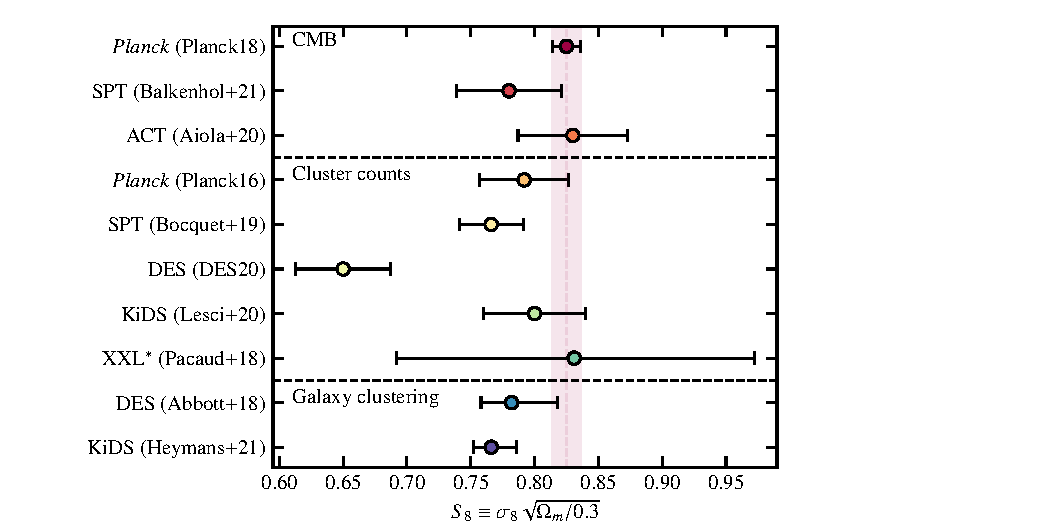
\includegraphics[width=.9\linewidth]{Figures/Chap_amas/S8.pdf}
    \caption{
        Contrainte sur la combinaison de paramètres cosmologiques $S_8$ obtenues par différentes mesures du CMB (haut), de comptage d'amas (milieu), et de distribution de galaxies (bas).
        De haut en bas, les résultats sont issus de \cite{planck_collaboration_planck_2020}\cite{balkenhol_constraints_2021}\cite{aiola_atacama_2020}\cite{planck_collaboration_planck_2016-2}\cite{bocquet_cluster_2019}\cite{des_collaboration_dark_2020}\cite{lesci_amico_2020}\cite{pacaud_xxl_2018}\cite{abbott_dark_2018}\cite{heymans_kids-1000_2021}. \\
        $^*$: incertitudes estimées graphiquement.
    }
    \label{fig:cluster_S8}
\end{figure*}

% ------------------------------------------------------------------------------------- %
\subsection{Relevés futurs}

Les décennies à venir promettent l'essor de la cosmologie avec des amas de galaxies, avec la réalisation d'un grand nombre de relevés du ciel, dans les longueurs d'onde de détection des amas, et avec une qualité de données sans précédent.

En optique, les relevés du Vera Rubin observatory et des satellites \textit{Euclid} et \textit{Roman} permettront la détection de centaines de milliers d'amas, avec des résolutions et des profondeurs permettant l'auto-étalonnage en masse à l'aide de lentillage faible jusqu'à haut redshift ($z \sim 2$, \eg\ \cite{lsst_science_collaboration_lsst_2009, sartoris_next_2016}).
En X, le relevé eROSITA anticipe la détection d'environ dix mille amas jusqu'à $z \sim 2$ \cite{merloni_erosita_2012}.
Enfin, en millimétrique, le Simons Observatory prévoit également la détection par effet SZ de $\sim 10^5$ amas, jusqu'à des redshifts $z \sim 3$, pouvant être exploité par auto-étalonnage de masse grâce au lentillage du CMB \cite{ade_simons_2019, louis_calibrating_2017}, et sera supplanté par CMB-S4 \cite{abazajian_cmb-s4_2016}.

Ainsi, les analyses cosmologiques basées sur les amas de galaxies bénéficieront très prochainement d'une grande diminution des incertitudes statistiques.
Dans ce cadre, les effets systématiques déjà importants deviendront dominants, et leur étude cruciale pour l'obtention de résultats compétitifs avec les autres sondes cosmologiques.
En effet, toute méconnaissance des outils nécessaires aux analyses cosmologiques, comme les relations d'échelle masse-observable, la forme de la fonction de masse, ou le profil de pression moyen des amas\footnote{discuté au chapitre suivant}, aura un impact sur les paramètres cosmologiques qui pourra ne plus être négligeable devant les effets statistiques (\eg\ \cite{ruppin_impact_2019, salvati_impact_2020, artis_impact_2021}).
Il sera alors important de maîtriser ces systématiques pour pouvoir tirer pleinement parti des jeux de données à venir.

% ------------------------------------------------------------------------------------- %
\subsection{Suivis dédiés d'échantillons d'amas}\label{sec:follow_ups}

Toute observation astronomique doit faire face à un compromis entre qualité des observations d'objets individuels et nombre d'objets détectés.
Dans le cadre des amas de galaxies, ce compromis permet de distinguer deux grandes catégories d'observations.
D'une part, les relevés d'amas sont basés sur l'observation homogène d'une portion du ciel, puis sur la détection des objets présents dans les observations.
Ils permettent l'établissement de grands catalogues nécessaires aux analyses cosmologiques comme le comptage d'amas, mais les données qui en sont issues ne permettent en général pas l'étude détaillée des propriétés physiques des amas.
Par exemple, dans le cas de l'effet SZ, le relevé \textit{Planck} \cite{planck_collaboration_planck_2016-2} a été réalisé avec une basse résolution angulaire de l'ordre de 7 arcmin.
Celle-ci ne permettant pas de résoudre les amas lointains, l'étude des propriétés thermodynamiques des amas individuels avec \textit{Planck} est limitée aux objets proches.
Or, la connaissance de ces propriétés est nécessaire aux analyses cosmologiques; aussi, une évolution de celles-ci avec le redshift, indétectable avec les données \textit{Planck} seules, aurait des conséquences sur les analyses cosmologiques basées sur ce catalogue (\eg\ \cite{ruppin_impact_2019}).

L'incapacité à mener des études détaillées des propriétés des amas à partir des relevés peut être compensée par un autre type d'observations: les suivis dédiés d'amas.
Ceux-ci permettent d'utiliser un instrument dédié à l'observation d'un plus petit nombre d'amas, mais fournissent des informations plus détaillées sur leurs propriétés.
Dans l'exemple de l'effet SZ, des instruments à haute résolution angulaire, comme les caméras NIKA2 \cite{adam_nika2_2018,perotto_calibration_2020} ou MUSTANG2 \cite{dicker_mustang2_2014}, permettent de cartographier l'effet SZ en direction d'amas lointains et d'étudier leurs propriétés thermodynamiques.
L'exemple du grand programme SZ de NIKA2 \cite{mayet_cluster_2020}, au sein duquel s'inscrit le travail effectué au cours de cette thèse, sera détaillé dans le chapitre suivant, en section \mypageref{sec:lpsz}.
Si l'échantillon suivi est représentatif de la population d'amas dans l'Univers, les propriétés observées des amas, comme la relation masse-observable, peuvent être généralisées à un relevé ne fournissant pas une information aussi détaillée.
De tels échantillons permettent donc l'étalonnage des outils nécessaires à la cosmologie sur un nombre restreint d'amas, avec une grande qualité de données, permettant l'étude des effets systématiques affectant les analyses cosmologiques basées sur les relevés d'amas.
Nous reviendrons sur ce point au chapitre \ref{chap:scaling}, dans lequel nous présenterons l'étalonnage de la relation d'échelle masse-observable pour le grand programme SZ de NIKA2.

% ------------------------------------------------------------------------------------- %
\subsection{Conclusions}

Dans ce chapitre, nous avons discuté des propriétés des amas de galaxies et détaillé l'utilisation de leur distribution dans l'Univers comme sonde cosmologique.
Au cours des dernières années, les différences entre les mesures des paramètres cosmologiques effectuées au travers de plusieurs sondes ont mis en évidence la nécessité de la maîtrise des effets systématiques propres aux analyses de chaque sonde.
Dans ce contexte, les amas de galaxies s'imposent comme une opportunité hors pair de maximiser le retour scientifique de chaque relevé du ciel.
En effet, de par la nature multilongueur d'onde de ces objets, la plupart des relevés du ciel sont en mesure de détecter des amas de galaxies: des observations du CMB, pouvant détecter des amas par effet SZ, aux relevés de galaxies, pouvant identifier les amas aux surdensités dans la distribution de ces dernières.
Ainsi, des relevés originellement prévus pour une sonde cosmologique peuvent utiliser les amas pour des résultats indépendants de leur sonde primaire, augmentant le pouvoir contraignant de leurs données sur les paramètres cosmologiques.

Nous avons vu que les relevés du futur permettraient une réduction drastique des incertitudes statistiques associées aux comptage d'amas.
La cosmologie avec des amas de galaxies entre donc dans une ère dans laquelle l'étude des effets systématiques sera cruciale à l'exploitation de relevés d'amas.
À l'heure actuelle, les effets systématiques dominants en cosmologie avec des amas proviennent pour la plupart de la méconnaissance des propriétés des amas et de leur évolution avec le redshift.
Dans ce contexte, la mise en place de suivis d'échantillons d'amas a le potentiel de fournir des études détaillées des effets systématiques liés à la détection et l'exploitation cosmologique des amas.

Les amas de galaxies promettent donc de jouer un rôle majeur dans la cosmologie des années à venir, et l'étude détaillée de leurs propriétés permettra d'augmenter leur potentiel en tant que sonde cosmologique.


% ------------------------------------------- %
\chapter{NIKA2 et son Grand Programme SZ}
\label{chap:nika2}
\minitoc
Nous avons vu au chapitre précédent que les amas de galaxies pouvaient être utilisés comme une sonde cosmologique.
Nous avons également présenté les outils nécessaires pour pouvoir mener de telles études, et l'intérêt des suivis dédiés d'échantillons d'amas dans l'étalonnage de ces outils.

C'est dans ce contexte que s'inscrit le grand programme SZ de NIKA2, au sein duquel cette thèse s'est déroulée.
NIKA2 est une caméra permettant d'observer le ciel dans le domaine millimétrique avec une résolution angulaire bien meilleure que celle des instruments utilisés pour construire des catalogues d'amas.
L'instrument a été construit à Grenoble par la collaboration NIKA2, et choisie par l'Institut de Radioastronomie Millimétrique (IRAM) pour être un instrument résident de son télescope de 30 mètres.
En retour de la construction de NIKA2, la collaboration s'est vu attribuer un total de 1300 heures d'observations avec l'instrument.
Le grand programme SZ est l'un des programmes bénéficiant de ce temps garanti.

Dans ce chapitre, nous décrivons la caméra NIKA2 et le grand programme SZ.
Nous décrirons tout d'abord quelques éléments caractéristiques du télescope de 30 mètres de l'IRAM et de la caméra NIKA2.
Nous détaillerons ensuite l'utilisation de l'instrument, ses caractéristiques, puis le grand programme SZ, de son utilisation des capacités de NIKA2 à ses objectifs scientifiques.
La dernière section sera consacrée à la base de données du grand programme SZ, dont la création fait partie de ce travail de thèse.

% ===================================================================================== %
\section{Le télescope de 30 mètres de l'IRAM}\label{sec:30m}

% ------------------------------------------------------------------------------------- %
\subsection{Localisation et conditions météorologiques}\label{sec:30m_geo}

Le télescope de 30 mètres de l'Institut de Radioastronomie Millimétrique (IRAM, figure \ref{fig:30m}) est installé dans la chaîne de montagnes de la Sierra Nevada, proche de Grenade, dans le sud de l'Espagne \cite{baars_iram_1987}.
Il est situé à une altitude de près de 2900 mètres au dessus du niveau de la mer, proche du sommet Pico Veleta; ses coordonnées sont 03\textdegree23'58.1''W, 37\textdegree04'05.6''N.

\begin{figure*}[t]
    \centering
    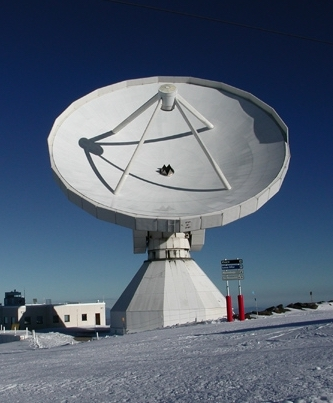
\includegraphics[height=7.5cm]{Figures/Chap_nk/30m_2.jpg}\hspace{10pt}
    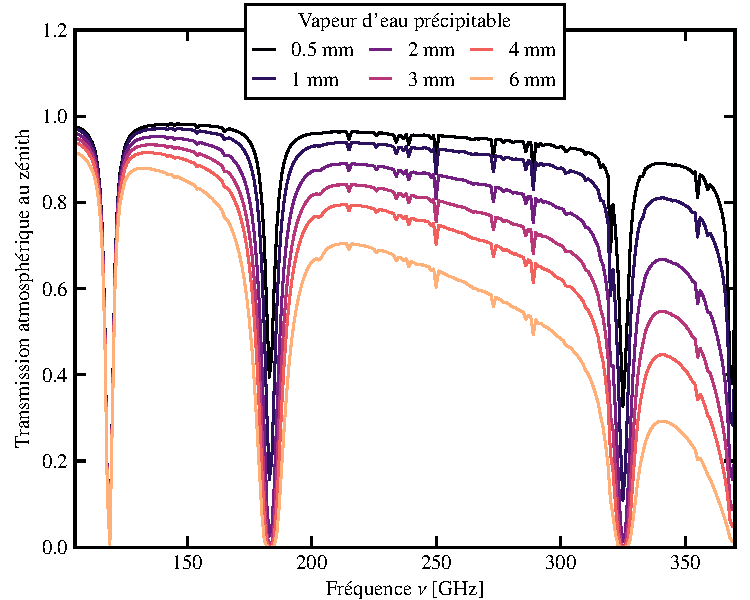
\includegraphics[height=7.5cm]{Figures/Chap_nk/atm_trans.pdf}
    \caption{
        \textbf{Gauche:} Photo du télescope de 30 mètres de l'IRAM.
        Crédit: \href{https://www.iram-institute.org/EN/photo-gallery.php?cat=2}{IRAM}.
        \textbf{Droite:} spectre de transmission atmosphérique en fonction de la quantité de vapeur d'eau précipitable, d'après le modèle de \myciteauthor{pardo_atmospheric_2001}.
    }
    \label{fig:30m}
\end{figure*}

Comme nous le verrons au chapitre suivant, l'une des sources de bruit principales dans les observations millimétriques est l'atmosphère.
Le bruit atmosphérique est principalement dû à son humidité.
Le site de Pico Veleta a donc été choisi pour son altitude, diminuant l'épaisseur de l'atmosphère traversée par les photons avant d'atteindre le télescope, mais également pour ses conditions météorologiques, en particulier son faible taux d'humidité.
Le spectre de transmission de l'atmosphère, calculé à l'aide du modèle de \myciteauthor{pardo_atmospheric_2001}, est représenté pour différentes valeurs de vapeur d'eau précipitable, correspondant à la quantité d'eau présente dans l'atmosphère.
On peut voir que pour des fréquences entre $100$ et $300$ GHz, la transmission est modulée par un continuum, dont la transmission diminue avec l'humidité, et par la présence de raies d'absorption (du dioxygène à $\sim 118$ GHz et de l'eau à $\sim 185$ et $325$ GHz).
Ces raies délimitent les gammes de longueurs d'onde observables depuis le sol, nommées fenêtres d'observation, centrées autour de $90$, $150$, $250$, et $350$ GHz.

En moyenne, les valeurs typiques de vapeur d'eau précipitable au télescope de 30 mètres sont de 7 mm en été, et de 3 mm en hiver.
En effet, la température de l'atmosphère est plus élevée l'été, augmentant la valeur de pression de vapeur saturante et donc la quantité d'eau qu'elle peut contenir.
Le télescope suit l'évolution de la quantité d'eau en temps réel en mesurant l'opacité atmosphérique au zénith $\tau_\nu$ grâce à un instrument résident dit taumètre, définie de façon à ce que la transmission de l'atmosphère $T_\nu$ à une fréquence $\nu$ soit
\begin{equation}
    \label{eq:tau_trans}
    T_\nu = \exp(- \tau_\nu / \sin(el)),
\end{equation}
où $el$ est l'élévation de l'objet observé. \\
L'opacité usuellement mesurée est $\tau_{225}$, à une fréquence de $225$ GHz, et vaut en moyenne $0.2$ en hiver et $0.5$ en été au télescope de 30 mètres.

La partie du ciel observable par le télescope est limitée au nord de la sphère céleste.
En effet, les objets de déclinaison inférieure à -20\textdegree\ en coordonnées équatoriales n'y atteignent jamais des élévations supérieures à 30\textdegree.
À de telles élévations, la couche d'atmosphère traversée par les rayons incidents est épaisse, et le poids du télescope commence à nuire à sa précision de pointage et affecter la forme de son lobe.
Les déclinaisons inférieures à -20\textdegree\ sont donc considérées comme inaccessibles pour le télescope.
Cela empêche l'observation d'amas découverts dans certaines régions des relevés réalisés dans l'hémisphère sud.
Comme le montre la figure \ref{fig:30m_sky}, une conséquence notable est l'impossibilité d'utiliser le télescope de 30 mètres pour le suivis d'amas des catalogues SPT \cite{bleem_galaxy_2015,bleem_sptpol_2020}, de même qu'environ la moitié du catalogue ACT \cite{hilton_atacama_2021}.
C'est la raison pour laquelle les amas de galaxies suivis par le grand programme SZ de NIKA2\footnote{Voir section \mypageref{sec:lpsz}} sont principalement issus du catalogue \textit{Planck}, couvrant tout le ciel, et de quelques uns des amas les plus au nord du catalogue ACT.

\begin{figure*}[t]
    \centering
    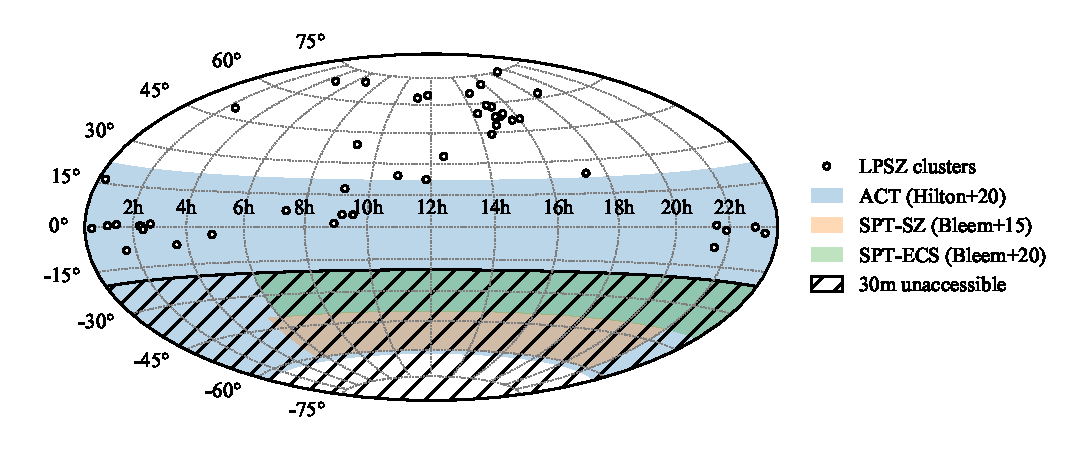
\includegraphics[width=.9\linewidth]{Figures/Chap_nk/footprints.pdf}
    \caption{
        Couvertures spatiales des relevés ACT (bleu, \cite{hilton_atacama_2021}) et SPT (orange et vert \cite{bleem_galaxy_2015,bleem_sptpol_2020}) en coordonnées équatoriales.
        Les axes horizontaux et verticaux représentent respectivement l'ascension droite et la déclinaison.
        La région hachurée marque les déclinaisons inaccessibles par le télescope de 30 mètres de l'IRAM.
        Les points représentent les coordonnées des amas du grand programme SZ de NIKA2 (voir section \ref{sec:lpsz} page \pageref{sec:lpsz}).
    }
    \label{fig:30m_sky}
\end{figure*}

% ------------------------------------------------------------------------------------- %
\subsection{Caractéristiques instrumentales}\label{sec:30m_opt}

Le télescope est constitué d'un miroir primaire paraboloïde de 30 mètres de diamètre, composé de panneaux d'aluminium et de polyuréthane \cite{baars_iram_1987}.
Afin de minimiser les variations de température induites par le lever et le coucher du soleil, qui entrainent une déformation du miroir primaire, ce dernier est activement thermalisé \cite{baars_thermal_1988} et peint de manière à réfléchir le rayonnement infrarouge.
Le miroir secondaire de 2 mètres de diamètre est maintenu à une distance de 10.5 mètres du primaire, égale à la distance focale de ce dernier.
L'ensemble est couplé à une cabine Nasmyth et installé sur une monture alt-azimuthale, pour une masse totale d'environ 800 tonnes.
Le télescope est présenté en figure \ref{fig:30m}.

Les rayons lumineux arrivent donc sur le miroir primaire du télescope, sont réfléchis par celui-ci vers le miroir secondaire, qui à son tour les redirige vers le vertex au centre du miroir primaire par lequel les faisceaux pénètrent dans la cabine.
La réponse angulaire du télescope, nommée \textit{lobe instrumental}, décrit la distribution du signal optique attendu à la sortie de ce vertex.
Dans le cas d'un signal monochromatique issu d'une source ponctuelle, cette réponse angulaire est donnée par la tâche d'Airy du miroir primaire à travers l'ouverture du vertex.
La largeur de celle-ci, déterminée par la largeur à mi-hauteur du pic principal, vaut $\theta = {\rm arcsin}(1.029 \times \lambda / D) =$ 14.1 et 8.2 arcsec pour des rayonnements monochromatiques de fréquences 150 et 260 GHz respectivement.
En pratique, le rayonnement incident est polychromatique, et ses multiples réflexions induisent un élargissement du lobe.
C'est la raison pour laquelle les différents instruments récepteurs dans la cabine du télescope ont des résolutions angulaires effectives moins bonnes que ces valeurs.

% ===================================================================================== %
\section{La caméra NIKA2}

La caméra NIKA2 (\textit{New IRAM KID arrays 2}) constitue l'instrument principal utilisé au cours de cette thèse.
Elle a été conçue par la collaboration internationale NIKA2, centrée à Grenoble, dans l'objectif de répondre à un appel d'offre de l'IRAM pour un nouvel instrument résident au télescope de 30 mètres.
Dans cette section, nous présentons brièvement l'instrument et son fonctionnement.
Plus de détails peuvent être trouvés dans \cite{adam_nika2_2018,perotto_calibration_2020}.
% ------------------------------------------------------------------------------------- %
\subsection{Détecteurs à inductance cinétique}\label{sec:kids}

Les détecteurs utilisés par NIKA2 sont des détecteurs à inductance cinétique (KID, pour \textit{kinetic indictance detectors}, \cite{day_broadband_2003,roesch_development_2012}).
Leur utilisation est l'une des spécificités de NIKA2, puisque la plupart des instruments millimétriques utilisent des détecteurs bolométriques.

Les KID sont des détecteurs supraconducteurs.
Ils sont constitués d'un matériau caractérisé par une température critique $T_c$ en dessous de laquelle les électrons sont séparés en deux populations: d'une part, des électrons appariés en \textit{paires de Cooper}, et d'autre part des électrons libres, nommés \textit{quasi-particules}.
La densité de paires de Cooper $n_s$ est alors donnée en fonction de la température $T$ par \cite{gorter_supraconductivity_1934}:
\begin{equation}
    \label{eq:cooper_dens}
    \frac{n_s}{n} = 1 - \left(\frac{T}{T_c}\right)^4,
\end{equation}
où $n$ est la densité totale des porteurs de charges, quasi-particules et paires de Cooper. \\
Les paires de Cooper forment des condensats de Bose-Einstein, pouvant être brisée par une énergie dite de \textit{gap}, notée $2\Delta$, et pouvant être calculée dans le cadre de la théorie Bardeen-Cooper-Schrieffer \cite{bardeen_microscopic_1957,bardeen_theory_1957} comme:
\begin{equation}
    2\Delta \simeq 3.53 \, k_\textsc{b} T_c.
\end{equation}
D'après l'équation (\ref{eq:cooper_dens}), pour des températures $T \ll T_c$, la majorité des charges est donc portée par des paires de Cooper ($n_s \simeq n$).
Alors, des photons incidents d'énergie supérieure au \textit{gap} $2\Delta$ pourront briser ces paires et changer la distribution des porteurs de charges entre paires de Cooper et quasi-particules.

Lorsqu'un supraconducteur est traversé par un courant électrique, la conduction peut être assurée par chacun des porteurs de charges.
Dans le cas d'un courant alternatif cependant, les paires de Cooper sont sujettes à une inertie, qui freine leur mouvement, et s'oppose donc à la conduction.
Ce phénomène crée une inductance qualifiée de cinétique $L_k$ dans le matériau, dont l'impédance s'écrit alors $Z = R_{qp} + i\omega L_k$, où $R_{qp}$ est la résistance liée aux quasi-particules, et $\omega$ la pulsation du courant alternatif.
Il apparaît naturellement qu'une variation de densité de paires de Cooper, par brisure de certaines d'entre elles par des photons incidents, créera une variation d'inductance cinétique $\delta L_k$.
Celle-ci est inversement proportionnelle à la variation de densité de paires de Cooper, et donc proportionnelle à la variation de puissance optique incidente (voir par exemple \cite{day_broadband_2003} pour une démonstration).

Le fonctionnement des KID est basé sur la mesure de variation de fréquence de résonance induite par un changement de puissance optique reçue.
Les détecteurs de NIKA2 sont des détecteurs à inductance de type LEKID (\textit{Lumped Element KID}, \cite{roesch_development_2012}).
Chaque KID est un circuit résonant de type RLC, constitué d'une partie capacitive $C$, d'un méandre inductif servant d'absorbeur de flux, d'inductance géométrique $L_g$ s'ajoutant à l'inductance cinétique $L_k$, et d'une résistance $R$.
La fréquence de résonance d'un KID est donc donnée par:
\begin{equation}
    \label{eq:kids_freq}
    f = \frac{1}{2\pi \sqrt{(L_g + L_k)C}}.
\end{equation}
Ainsi, une variation de puissance optique incidente sur le détecteur va induire un changement de la proportion de porteurs de charges sous forme de paires de Cooper, ce qui créera une variation de l'inductance cinétique du supraconducteur, qui aura à son tour pour conséquence une modification de la fréquence de résonance du détecteur.
La dérivation de l'équation (\ref{eq:kids_freq}) par rapport à l'inductance cinétique $L_k$ permet d'exprimer cette variation de fréquence de résonance par rapport au changement d'inductance cinétique:
\begin{equation}
    \delta f = \pdv{f}{L_k} \delta L_k = -2 \pi^2 C \, f^{\;3} \delta L_k.
\end{equation}
Comme nous l'avons vu précédemment, le changement d'inductance cinétique est inversement proportionnel à la variation de puissance optique incidente; ainsi,
\begin{equation}
    \delta f \propto \delta L_k \propto -\delta P_{\rm opt}.
\end{equation}

La mesure de cette variation de fréquence de résonance permet donc de remonter à la variation de puissance optique l'ayant causée.
Afin de mesurer $\delta f$, les détecteurs sont couplés à des lignes de transmission, parcourues par un signal alternatif.
Celles-ci sont couplées inductivement aux méandres des KID: le signal transmis est donc affecté par la présence de chaque détecteur.
La variation en phase et en amplitude du signal de la ligne de transmission due à la présence d'un KID est liée à la fréquence de résonance de ce dernier.
Ainsi, la mesure de la phase et de l'amplitude du signal de sortie de la ligne de lecture permet de reconstruire la variation de fréquence de résonance des détecteurs présents le long de cette ligne, et \textit{in fine} à la variation de puissance lumineuse.

Comme le montre l'équation (\ref{eq:kids_freq}), la fréquence de résonance d'un KID est liée à la capacité de son condenseur $C$.
Ainsi, la fréquence de résonance de chaque détecteur peut être ajustée par contrôle des des propriétés géométriques du condenseur.
Cette caractéristique fait des KID des détecteurs intrinsèquement adaptés au multiplexage: un grand nombre de détecteurs peuvent avoir des fréquences de résonance différentes et être montés sur une même ligne de lecture.
Par conséquent, la quantité de câbles électroniques nécessaires à la transmission des signaux d'une matrice de détecteurs est fortement diminuée par rapport aux bolomètres, nécessitant une ligne de lecture par détecteur.
Au vu des contraintes cryogéniques importantes pour les détecteurs, une augmentation du nombre de détecteurs lisibles par une ligne de lecture permet l'augmentation du nombre de détecteurs sans pour autant augmenter le nombre de câbles devant sortir du cryostat.
Cette qualité fait des KID des détecteurs particulièrement compétitifs.

Un des KID de la caméra NIKA et une matrice de détecteurs installée dans NIKA2 sont présentés en figure \ref{fig:nk_kids}.
Le panneau de gauche montre les différentes parties du détecteur: le condensateur (en haut), et le méandre inductif, occupant la majorité de la surface du détecteur et dans lequel les photons sont absorbés et peuvent briser des paires de Cooper.
On voit également la ligne de transmission utilisée pour lire le détecteur qui en longe le côté inférieur.
Sur le panneau droit, on voit une des matrices de 1140 KID de NIKA2.
Les détecteurs individuels ne sont pas distinguables, mais on peut voir les huit lignes de transmission utilisées pour la lecture des 1140 détecteurs.

\begin{figure*}[t]
    \centering
    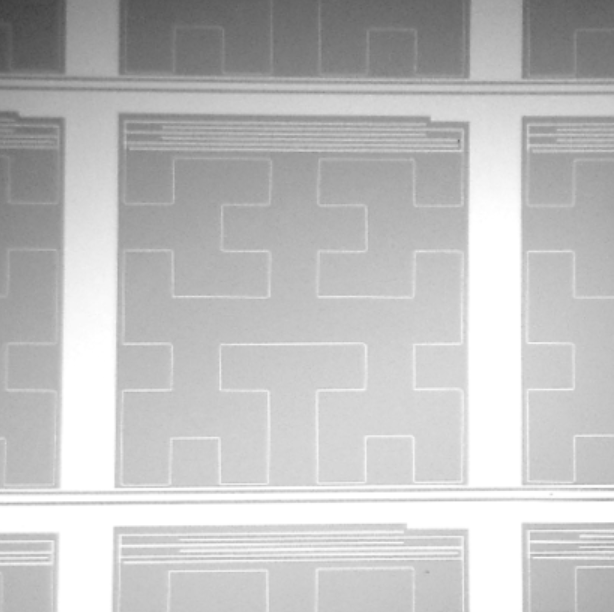
\includegraphics[height=7cm]{Figures/Chap_nk/fig3_AB.png}
    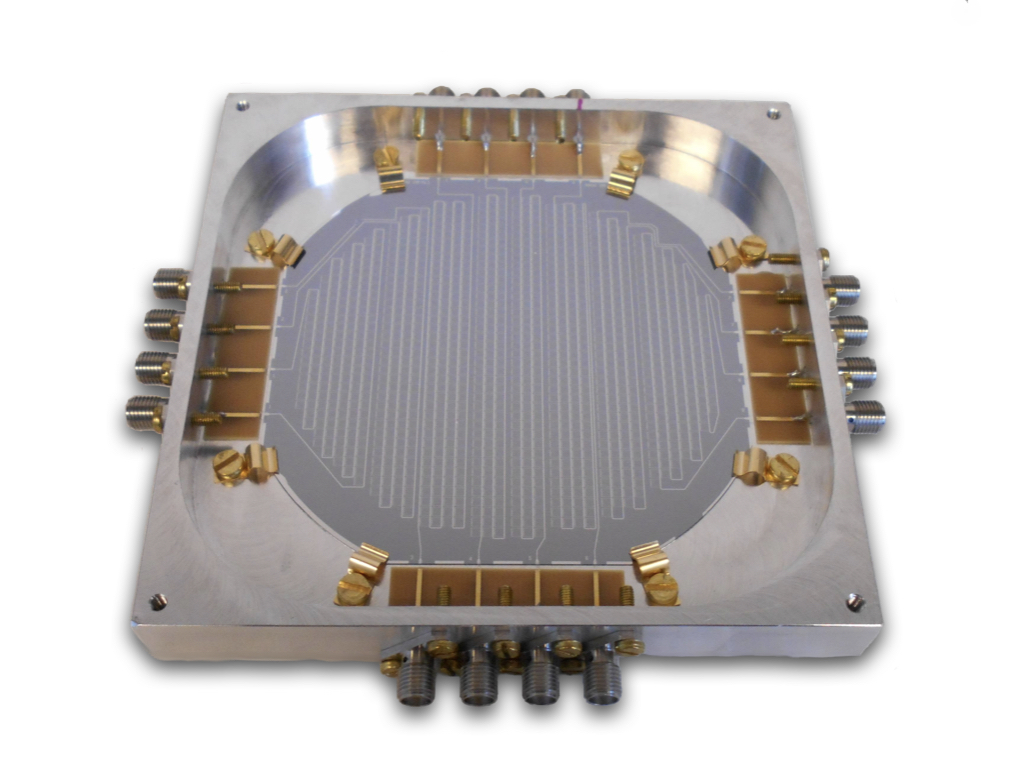
\includegraphics[height=7cm]{Figures/Chap_nk/1mm_array.jpeg}
    \caption{
        \textbf{Gauche:} Image d'un détecteur KID de NIKA, de taille 2.3 mm $\times$ 2.3 mm.
        Le méandre inductif du détecteur couvre la plupart de sa surface, tandis que la partie capacitive $C$ est située dans la partie haut du détecteur.
        \textbf{Droite:} Matrice de KID dans la bande à 260 GHz de NIKA2, comportant 1140 KID et 8 lignes de transmission.
        Figures extraites de \cite{adam_nika2_2018}.
    }
    \label{fig:nk_kids}
\end{figure*}


% ------------------------------------------------------------------------------------- %
\subsection{Éléments clés de la caméra NIKA2}

Les KID de NIKA2 sont constitués d'une couche mince d'aluminium d'environ 18 nm d'épaisseur.
La température critique de l'aluminium étant de $T_c = 1.19 \;\unit{K}$, l'énergie du \textit{gap} vaut $2\Delta \simeq 0.36 \;\unit{meV}$, correspondant à des photons à une fréquence de l'ordre de 90 GHz.
De tels détecteurs sont donc tout à fait appropriés pour la mesure du fond diffus cosmologique et de l'effet SZ (cf. figure \ref{fig:tsz_spec}).

La caméra NIKA2 est dotée de trois matrices de KID.
Deux matrices (A1 et A3), chacune composée de 1140 détecteurs, sont placées derrière une lame dichroïque transmettant une gamme de fréquence centrée à 260 GHz.
La troisième (A2) est quant à elle dédiée à l'observation de photons de fréquence autour de 150 GHz.
Les deux bandes passantes de NIKA2 sont donc adaptées aux fenêtres d'observation disponibles au vu de la transmission atmosphérique (cf. figure \ref{fig:30m}).
Elles sont illustrées sur la figure \ref{fig:nk_bp}.
Il y apparait que les bandes passantes de NIKA2 exploitent parfaitement les fenêtres spectrales disponibles pour des observations millimétriques depuis le sol, de même que la dépendance spectrale de l'effet Sunyaev-Zeldovich, avec une bande de chaque côté du zéro de la distorsion spectrale (cf. section \ref{sec:sz}).
Ce point sera abordé plus en détail en \mypageref{sec:lpsz}.

\begin{figure*}[t]
    \centering
    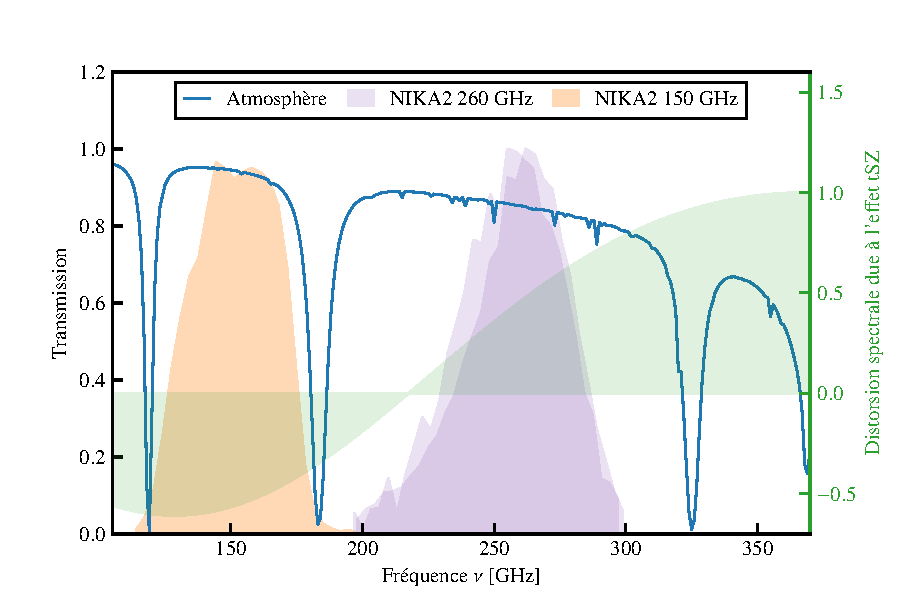
\includegraphics[width=.8\linewidth]{Figures/Chap_nk/bandpasses.pdf}
    \caption{
        Bandes passantes de NIKA2 à 260 GHz (violet) et 150 GHz (orange).
        La transmission atmosphérique calculée à partir du modèle de \myciteauthor{pardo_atmospheric_2001} pour 2 mm de vapeur d'eau précipitable est également représentée en bleu.
        La distorsion spectrale due à l'effet tSZ est montrée en vert.
    }
    \label{fig:nk_bp}
\end{figure*}

Comme nous l'avons discuté en \ref{sec:kids}, le fonctionnement des détecteurs à inductance cinétique requiert que ceux-ci soient refroidis à une température inférieure à leur température critique.
Dans le cas de NIKA2, cette condition est assurée par un cryostat, maintenant les détecteurs à une température d'environ 150 mK, bien en deçà de la température critique de l'aluminium.

Un système optique dévie les rayons lumineux focalisés par le télescope (cf. section \ref{sec:30m_opt}) vers les matrices de KID.
Celui-ci est tout d'abord composé de quatre miroirs dans la cabine du télescope, dirigeant les rayons issus du miroir secondaire du télescope vers le cryostat de NIKA2.
Une fois qu'ils ont pénétré le cryostat, les rayons lumineux sont réfléchis par une succession de miroirs refroidis, puis traversent un filtre dichroïque, séparant la lumière en deux.
Celui-ci permet de diriger une partie des rayons incidents vers la matrice de KID à 150 GHz, et l'autre vers les matrices à 260 GHz.
La présence des deux matrices à 260 GHz et d'un élément polariseur permet à NIKA2 d'être sensible à la polarisation des photons incidents à 260 GHz.
Dans le travail développé au cours de cette thèse, cette capacité ne sera pas exploitée, et les données issues des deux matrices à 260 GHz sont combinées en une unique carte du ciel à cette fréquence.

% ===================================================================================== %
\section{Observations avec NIKA2} \label{sec:nk_obs}

Les observations avec la caméra NIKA2 réalisées et étudiées au cours de cette thèse suivent une procédure précise, dont le but est la production de cartes fidèles du ciel.
Dans cette section, nous détaillons cette procédure, ainsi que les performances de l'instrument.
L'étape suivante, visant à isoler les signaux astrophysiques des différents contaminants, sera détaillée au chapitre suivant.

% ------------------------------------------------------------------------------------- %
\subsection{Balayage du ciel et données ordonnées en temps} \label{sec:nk_otf_toi}

Comme nous l'avons vu dans la section précédente, les KID permettent de mesurer une variation de puissance lumineuse.
Ainsi, ils sont moins adaptés à la mesure de signaux stationnaires qu'à celle de signaux variant dans le temps.
Pour pouvoir mesurer des signaux stationnaires, tels que les signaux astrophysiques étudiés au cours de cette thèse, il est donc nécessaire d'adopter une stratégie visant à moduler le signal d'intérêt dans le temps.

Dans le cas de NIKA2, cet objectif est accompli en balayant le ciel par des \textit{scans}, dont le principe est le suivant.
Le télescope se déplace suivant une trajectoire déterminée, de sorte à ce que la position sur le ciel d'un détecteur de référence soit connue à tout instant.
Chacun des KID de NIKA2 enregistre alors la variation de la puissance lumineuse qu'il reçoit au cours du temps.
Les données enregistrées sont par conséquent ordonnées en temps, et nommées TOI pour \textit{Time Ordered Information}.
Une fois le balayage terminé, une matrice de pointage est calculée, donnant la position de chaque KID sur le ciel au cours du temps à partir du pointage de référence du télescope et de la position relative de chaque KID par rapport à ce centre de référence (la mesure de celle-ci sera détaillée en \ref{sec:focal_plane_reconstruction}).
La matrice de pointage permet alors de projeter les TOIs de chaque KID en cartes du ciel.
En plus de moduler temporellement le signal pour le rendre détectable par les KID, cette méthode permet d'exploiter la redondance du signal et les corrélations entres les différentes sources de bruit.
Comme nous le verrons au chapitre suivant, cette redondance facilite la différenciation du signal et du bruit dans les données.

\begin{figure*}[t]
    \centering
    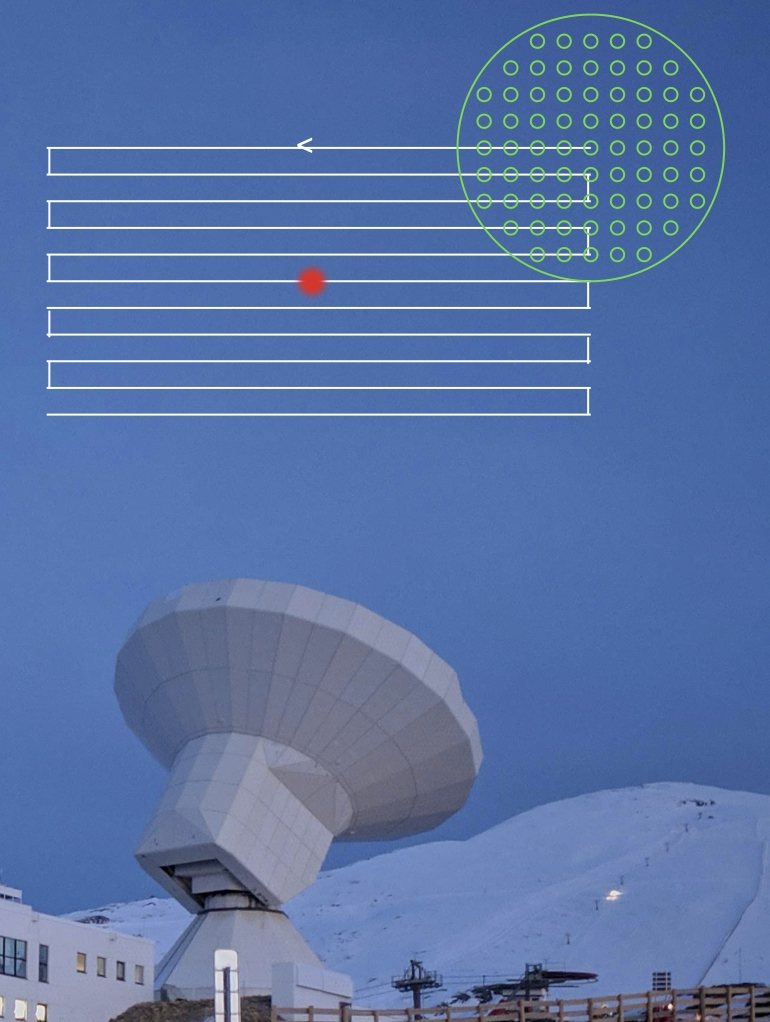
\includegraphics[height=8cm]{Figures/Chap_nk/otf_telescope_source.jpg}\hspace{10pt}
    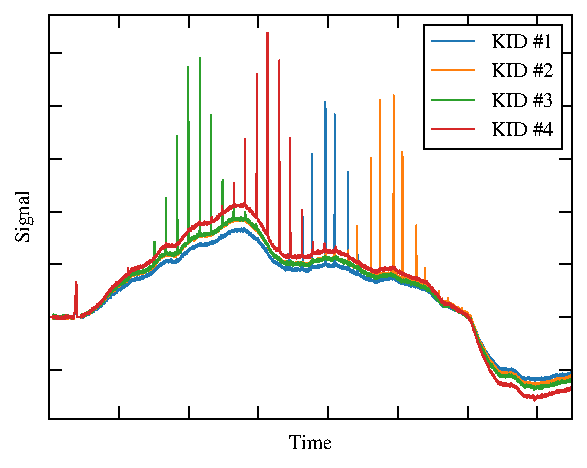
\includegraphics[height=7.5cm]{Figures/Chap_nk/tois.pdf}
    \caption{
        \textbf{Gauche:} illustration du mouvement effectué par le télescope dans le ciel (en blanc) lors d'un scan OTF.
        La matrice de détecteurs est représentée en vert, et la source observée en rouge.
        \textbf{Droite:} représentation des données ordonnées en temps obtenues par scan d'Uranus pour trois KID.
        La détection de la source se manifeste par un pic de signal détecté.
    }
    \label{fig:nk_otf_toi}
\end{figure*}

La trajectoire suivie par le télescope pour réaliser un scan est nommée stratégie de scan.
Le choix de celle-ci est capital, puisqu'il a un grand impact sur la capacité à reconstruire le signal astrophysique (comme nous le verrons dans le chapitre suivant).
Dans le cas des observations de l'effet SZ discutées au cours de cette thèse, la stratégie employée est basée sur la réalisation de scans OTF (pour \textit{on the fly}): une successions de \textit{subscans} rectilignes parallèles en coordonnées équatoriales sont effectués, espacés d'un pas constant.
Cette stratégie induit un mouvement du télescope en forme de serpentin, illustrée sur le panneau gauche de la figure \ref{fig:nk_otf_toi}.
Les données ordonnées en temps obtenues pour un tel \textit{scan} sur une source ponctuelle brillante (Uranus) sont représentées sur le panneau droit de la figure \ref{fig:nk_otf_toi}.
Étant données les différentes positions des détecteurs dans le plan focal, ces derniers ne détectent pas le passage de la source au même moment, ce qui se manifeste par un décalage en temps du signal de la source.
Les observations du grand programme SZ sont effectuées par groupes de quatre scans, à des angles de $0^\circ$, $45^\circ$, $90^\circ$, et $135^\circ$ par rapport à l'axe des ascensions droites, afin de maximiser l'isotropie de la couverture du ciel.
Ce point sera discuté plus en détail au chapitre suivant.

% ------------------------------------------------------------------------------------- %
\subsection{Reconstruction du plan focal}\label{sec:focal_plane_reconstruction}

Le grand nombre de détecteurs présents sur une même ligne de lecture peut causer des difficultés à isoler les signaux provenant de chaque détecteur.
En particulier, la lecture de la fréquence de résonance d'un détecteur ne permet pas de connaître sa position dans la matrice.
De plus, la fréquence de résonance de certains détecteurs peut ne pas être trouvée, ou bien être trop proche de celle d'un détecteur voisin, auquel cas les signaux en provenance des deux KID sont incorrectement associés à un seul détecteur.
Il est donc nécessaire, avant d'observer, de reconstruire le plan focal de la caméra en associant chaque fréquence de résonance à un KID, permettant de connaître sa position et d'identifier les détecteurs invalides.

Pour cela, une carte profonde d'une source brillante, par exemple une planète comme Uranus, est réalisée de façon à ce qu'une carte de la source puisse être construite pour chaque détecteur.
Ces cartes, nommées \textit{beammaps}, ont plusieurs vertus.
Elles permettent d'une part, pour chaque détecteur, de connaître sa position dans la matrice par rapport à un KID de référence, ce qui permettra la reconstruction des observations du ciel détaillée par la suite.
Elles permettent également l'identification des détecteurs en diaphonie, pour lesquels deux sources apparaissent sur une même carte, de même que les détecteurs hors résonance.
Les gains des KID, quantifiant l'étalonnage relatif de chaque détecteur, sont également calculés à partir de ces cartes grâce au rapport entre le flux connu de la source et la variation de fréquence de résonance correspondante pour chaque détecteur.
Enfin, ces cartes sont utilisées pour la mesure du lobe instrumental observé par chacun des détecteurs, discutée en \mypageref{sec:nk_perf}.

% ------------------------------------------------------------------------------------- %
\subsection{Pointage et focalisation}\label{sec:pointing_focus}

Avant d'observer des sources, il est nécessaire de s'assurer que le télescope est à même de livrer des observations fidèles du ciel.
Il faut donc s'assurer que le KID de référence est correctement aligné avec l'axe optique du télescope, et que ce dernier est correctement focalisé.

Le pointage du télescope est vérifié en réalisant un mouvement d'aller-retour sur une source, tout d'abord en azimut, puis en élévation, formant une croix dans le plan du ciel.
Des profils Gaussiens sont ajustés sur les TOIs d'un détecteur de référence au centre des matrices de NIKA2.
La position de la source dans le ciel étant connue, il est alors possible d'associer des coordonnées célestes au détecteur de référence, et par extension aux autres KID des matrices de NIKA2.
Un exemple de procédure de pointage est présenté en figure \ref{fig:nk_pointing}, illustrant la carte obtenue pour un pointage sur Uranus.
L'ajustement des profils de la source le long des axes des azimuts et élévations mesurés par le détecteur de référence (bas de la figure) permet de faire correspondre les coordonnées de chacun des détecteurs dans le plan focal avec ses coordonnées célestes\footnote{Notons que la procédure utilisée pour le pointage ajuste le profil de la source sur les TOI du KID de référence, alors que les profils représentés sur la figure \ref{fig:nk_pointing} sont ceux de la carte déjà projetée.}.

\begin{figure*}[t]
    \centering
    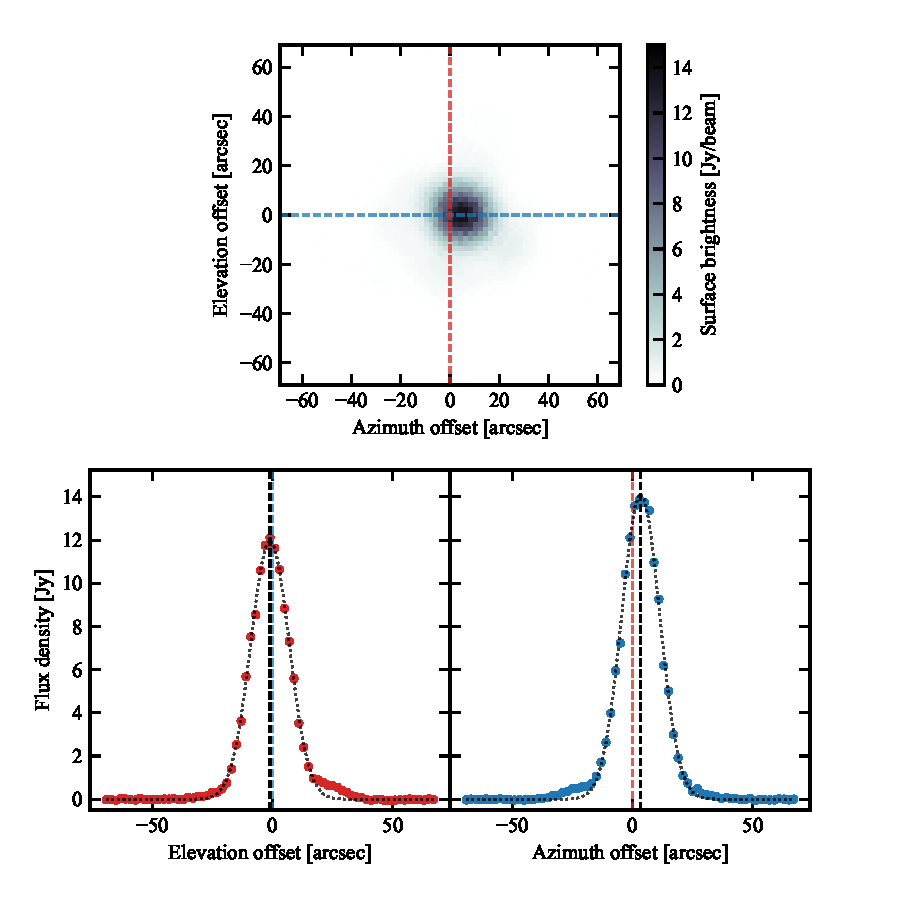
\includegraphics[width=.8\linewidth]{Figures/Chap_nk/pointing.pdf}
    \caption{
        Exemple de procédure de pointage.
        \textbf{Haut:} carte d'Uranus obtenue avec un scan en croix, suivant les directions des lignes bleue puis rouge, projetée en utilisant la matrice de pointage avant correction de pointage.
        \textbf{Bas:} profils de la planète le long de l'axe des élévations (\textit{gauche}) et des azimuts (\textit{droite}).
        L'ajustement des profils par une gaussienne (courbes pointillées noires) permet de mesurer le centre de la source dans les deux directions (lignes noires verticales).
        La différence entre la position de la source et celle du centre de la carte donne les corrections de pointage utilisées pour réaligner le KID de référence.
    }
    \label{fig:nk_pointing}
\end{figure*}

La focalisation du télescope quantifie l'accord entre la position du miroir secondaire et le point focal du miroir primaire.
Lorsque le télescope est défocalisé, c'est-à-dire lorsque le miroir secondaire est éloigné du point focal du primaire, les rayons ne sont pas réfléchis correctement vers le système optique, induisant des déformations de l'image reconstruite avec NIKA2, et notamment un élargissement du lobe.
Il faut alors positionner correctement le miroir secondaire.
Afin de connaître la position optimale de celui-ci, un scan OTF est effectué sur une source brillante pour cinq distances différentes entre les miroirs primaire et secondaire, espacées de $0.4 \;\unit{mm}$.
Les cartes obtenues à partir de ces observations sont créées et utilisées pour ajuster un modèle de lobe gaussien.
La procédure est illustrée en figure \ref{fig:nk_focus} avec la matrice à 150 GHz de NIKA2.
Cinq cartes d'Uranus sont produites (haut) et ajustées avec un modèle de lobe gaussien, permettant de mesurer la largeur du lobe et le flux de la source pour chacune des cartes.
Ces résultats sont ajustés avec une loi parabolique, dont le maximum donne les valeurs de la distance primaire-secondaire maximisant le flux et minimisant la largeur du lobe.
L'une ou l'autre de ces deux distances peut être choisie comme distance optimale pour la focalisation du télescope, selon la qualité de l'ajustement.
On note que les résultats des deux estimateurs sont en général très proches -- une différence de 0.03 mm est trouvée dans l'exemple de la figure \ref{fig:nk_focus}.

Un pointage correct est important pour toutes les observations réalisées avec NIKA2, incluant les observations de l'effet SZ.
Un mauvais pointage entraîne une connaissance imprécise de la position des détecteurs, et empêche donc la construction de cartographies fidèles du ciel.
Une erreur systématique sur le pointage de toutes les observations d'une source entraîne une mauvaise reconstruction des coordonnées du signal dans le ciel, qui a pour conséquence l'impossibilité de comparer des cartes NIKA2 avec des données issues d'autres instruments.
Comme nous le verrons dans les chapitres \ref{chap:panco} et \ref{chap:actj0215}, de telles comparaisons sont au cœur des analyses du grand programme SZ traitées dans cette thèse, et sont nécessaires à l'étude des propriétés thermodynamiques des amas de galaxies et des contaminants astrophysiques.
D'autre part, des imprécisions régulières (par exemple, variant d'un scan à l'autre) entraîne une dilution du signal, l'attribuant à des positions incorrectes, et donc un élargissement effectif du lobe de l'instrument.
Comme nous le verrons en section \mypageref{sec:lpsz}, la résolution angulaire de NIKA2 est l'un de ses principaux atouts pour la mesure de l'effet SZ.
La précision du pointage pouvant être dégradée par les mouvements du télescope, celui-ci est vérifié régulièrement au cours des observations, environ une fois par heure.
De même, comme le montre la figure \ref{fig:nk_focus}, une mauvaise focalisation du télescope entraîne un élargissement du lobe, et donc une dégradation de la résolution angulaire.
La focalisation variant principalement avec la géométrie du miroir primaire, qui se déforme avec les changements de température.
C'est pour cette raison que les observations diurnes avec NIKA2 doivent éviter l'illumination du miroir primaire avec le soleil, et que la focalisation est vérifiée à intervalles réguliers (toutes les heures de jour, et toutes les deux à trois heures la nuit).

\begin{figure*}[t]
    \centering
    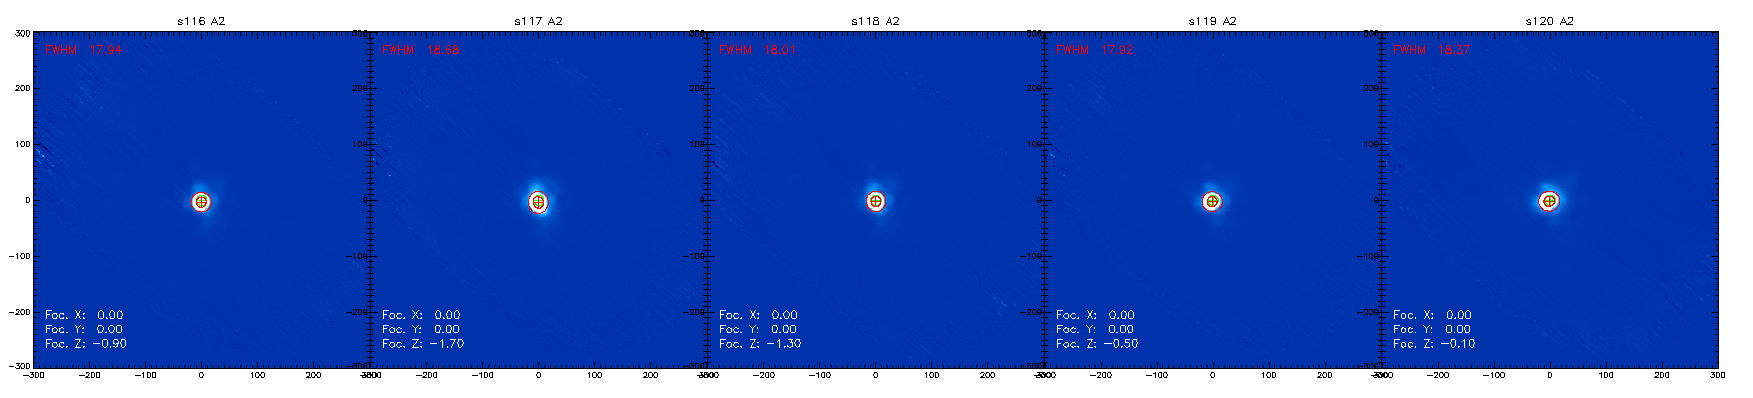
\includegraphics[width=.9\linewidth]{Figures/Chap_nk/focus_maps_crop.png}
    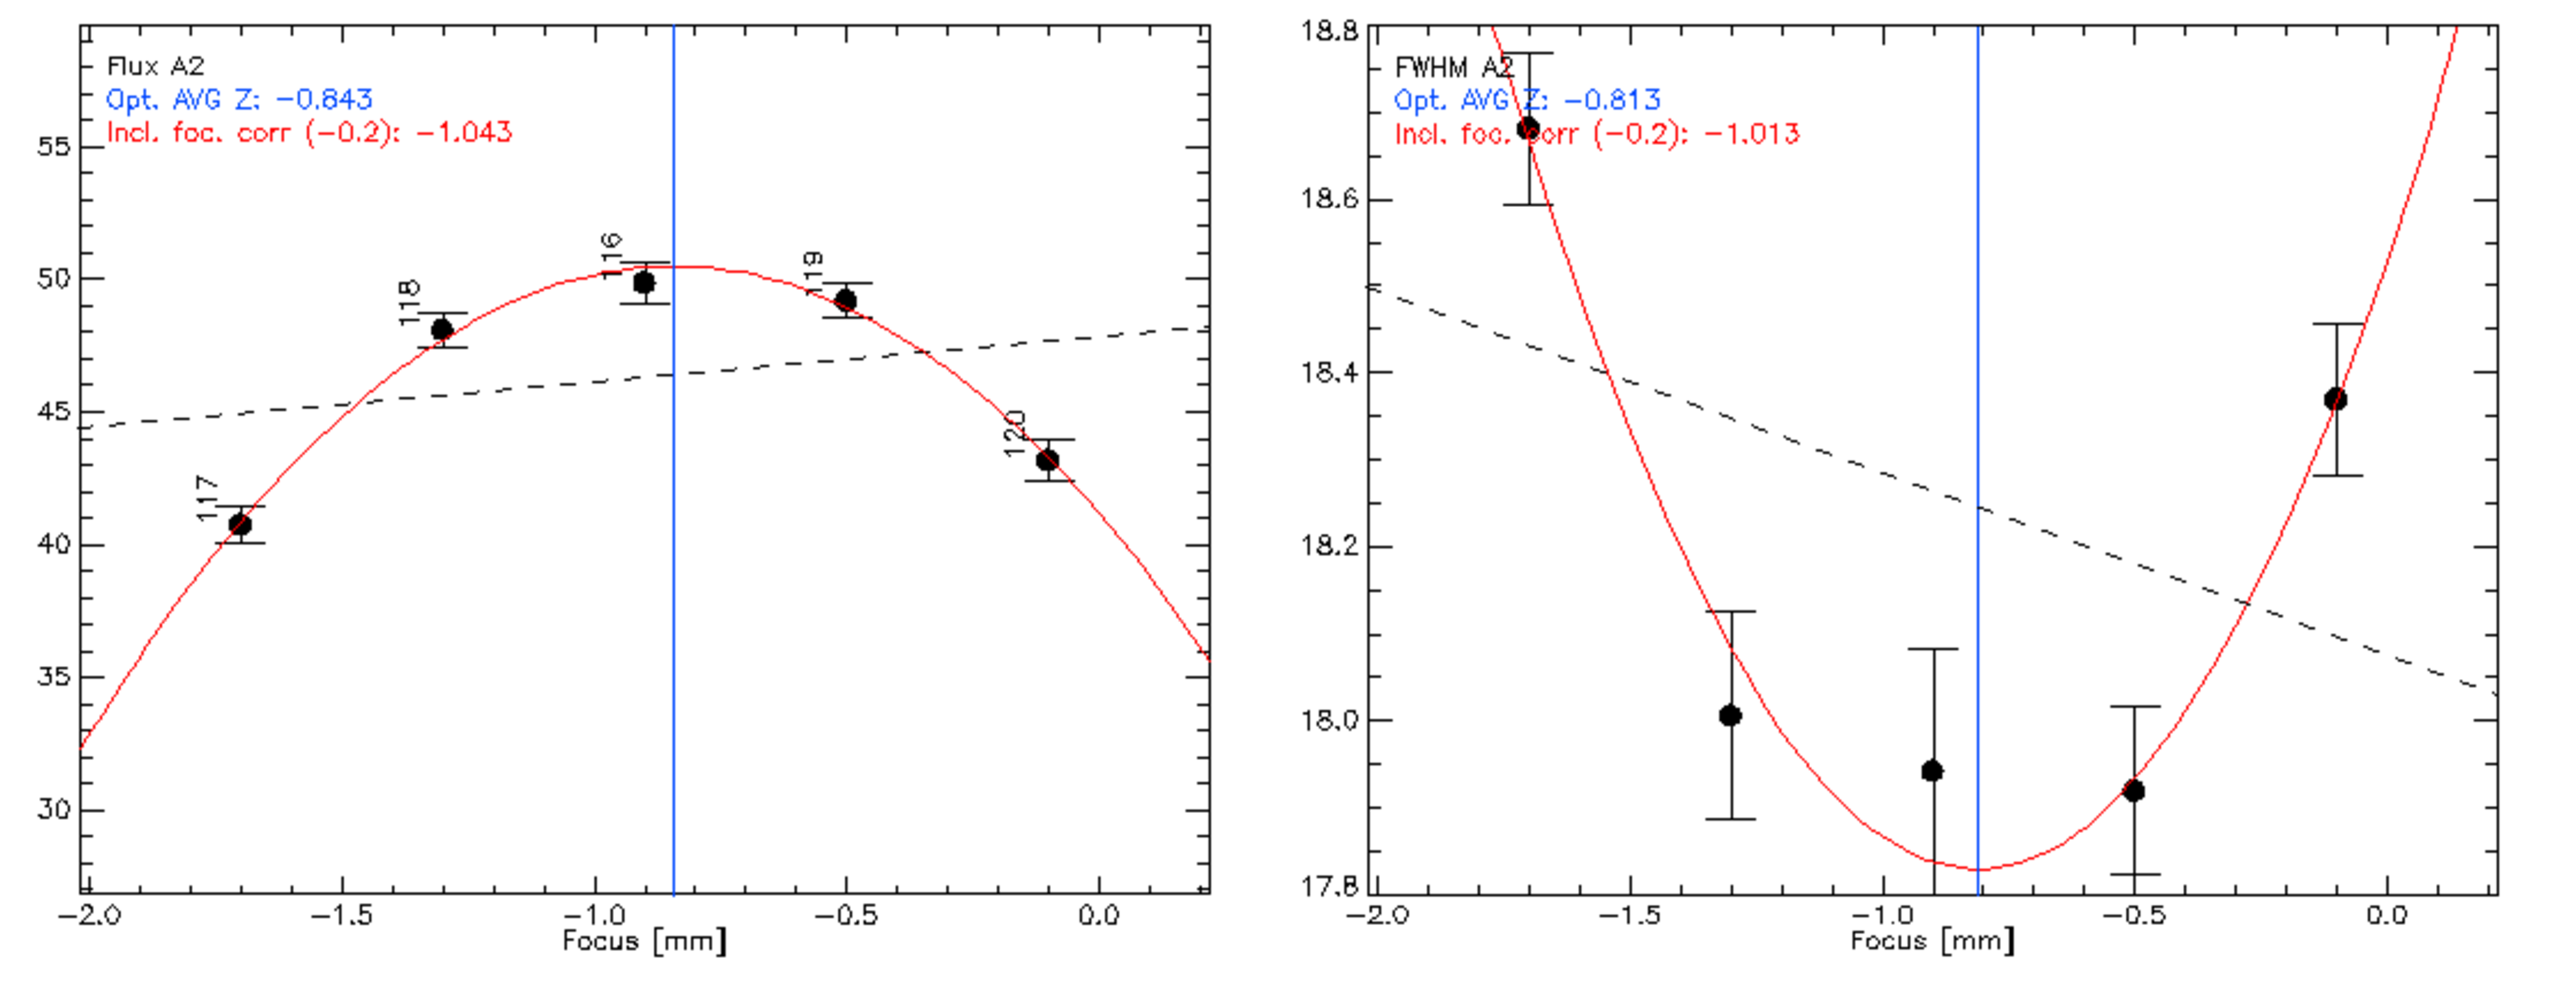
\includegraphics[width=.9\linewidth]{Figures/Chap_nk/focus_results_crop.pdf}
    \caption{
        Exemple de procédure de focalisation du télescope.
        \textbf{Haut:} cartes à 150 GHz d'Uranus obtenue pour cinq distances primaire-secondaire.
        \textbf{Bas:} Flux d'Uranus (\textit{gauche}) et largeur à mi-hauteur (\textit{droite}) mesurées dans chacune des cartes (noir).
        L'ajustement des points avec une loi parabolique (rouge) permet de mesurer la distance permettant une focalisation optimale du télescope (bleu).
    }
    \label{fig:nk_focus}
\end{figure*}

% ------------------------------------------------------------------------------------- %
\subsection{Performances instrumentales de NIKA2}\label{sec:nk_perf}

Les caractéristiques de NIKA2 ont été mesurées par la collaboration du même nom au cours de sa phase de \textit{commissioning}.
Ces mesures sont décrites avec un grand niveau de détail par \myciteauthor{perotto_calibration_2020}, et nous n'en donneront que les résultats principaux nécessaires à la description du travail effectué dans cette thèse.
La phase de \textit{commissioning} de l'instrument a eu lieu entre Octobre 2015 et Avril 2017.
Elle a permis de mesurer avec précision les caractéristiques de l'instrument, telles que son lobe et sa sensibilité.
La mesure des performances de l'instrument a quant à elle eu lieu au cours de trois campagnes d'observations en Février et Octobre 2017 et Janvier 2018.
Les résultats principaux de ces mesures sont consignés dans la table \ref{tab:nk_specs}, et nous détaillons ici brièvement la signification des caractéristiques et la méthode de calcul.

\begin{table}[t]
    \setlength{\tabcolsep}{15pt}
    \small
    \centering
    \begin{tabular}{l r r}
        \toprule
        Caractéristique & Matrices A1 et A3 & Matrice A2 \\
        \midrule
        \midrule
        \multicolumn{3}{c}{\itshape Bandes passantes} \\
        \midrule
        Longueur d'onde de référence [mm]   & 1.15 & 2.00 \\
        Fréquence de référence [GHz]        & 260  & 150  \\
        \midrule
        \multicolumn{3}{c}{\itshape Nombre de détecteurs} \\
        \midrule
        Nombre de détecteur présents        & $1140 \times 2$ & 616 \\
        Fraction de détecteurs valides [\%] & 84 & 90 \\
        \midrule
        \multicolumn{3}{c}{\itshape Résolution angulaire et champ de vue} \\
        \midrule
        Largeur à mi-hauteur (FWHM) du lobe principal [arcsec] & $11.1 \pm 0.2$ & $17.6 \pm 0.1$ \\
        Champ de vue instantané [arcmin]    & 6.5 & 6.5 \\
        \midrule
        \multicolumn{3}{c}{\itshape Incertitudes de pointage et d'étalonnage} \\
        \midrule
        Erreurs de pointage [arcsec] & $<3$ & $<3$ \\
        Incertitude sur l'étalonnage absolu [\%] & 5 & 5 \\
        Incertitude RMS sur l'étalonnage de sources ponctuelles [\%] & 5.7 & 3.0 \\
        \midrule
        \multicolumn{3}{c}{\itshape Sensibilité} \\
        \midrule
        NEFD [$\unit{mJy \cdot s^{1/2}}$]  & $30 \pm 3$ & $9 \pm 1$ \\
        \textit{Mapping speed} [$\unit{arcmin^2 \cdot mJy^{-2} \cdot h^{-1}}$] & $111 \pm 11$ & $1388 \pm 174$ \\
        \bottomrule
    \end{tabular}
    \caption{%
        Caractéristiques et performances instrumentales de NIKA2 mesurées par \myciteauthor{perotto_calibration_2020} (voir texte pour des explications sur la signification des termes).
    }
    \label{tab:nk_specs}
\end{table}

\subsubsection{Détecteurs valides} % -------------------------------------------------- %
Le nombre de détecteurs valides est évalué à l'aide des \textit{beammaps} décrites en \ref{sec:focal_plane_reconstruction}.
Sont considérés comme valides les détecteurs pour lesquels la mesure de la variation de fréquence de résonance lors du passage sur une source brillante permet de déduire une cartographie de cette source.
En d'autre termes, les détecteurs invalides incluent les détecteurs bruités dont la projection des données en temps ne permet pas d'identifier une source, ainsi que les détecteurs en diaphonie.
Il est à noter que l'invalidité d'un détecteur n'est pas définitive, et est liée à la mesure des fréquences de résonance par l'électronique de lecture et à la connaissance \prior\ de la position de ces fréquences de résonance dans le plan focal.
Ainsi, un détecteur non-valide ne l'est pas définitivement, et peut redevenir valide.
Ces valeurs sont de 84\% et 90\% à 260 et 150 GHz respectivement, montrant qu'une grande majorité des détecteurs peuvent être lus, et l'efficacité du multiplexage fréquentiel utilisé dans NIKA2.

\subsubsection{Lobe instrumental de NIKA2} % ------------------------------------------ %
La connaissance de la réponse angulaire de l'instrument est cruciale à la construction et à l'étalonnage des cartes du ciel.
Le lobe du couplage télescope-NIKA2 est une fonction complexe, dont la forme peut être modélisée de plusieurs façons.
Nous renvoyons le lecteur vers la section 6 de \cite{perotto_calibration_2020} pour plus de détails.
Le lobe principal, lié au pic central de la tache d'Airy du miroir primaire à travers l'ouverture du vertex, est modélisé comme une Gaussienne à deux dimensions, dont la largeur est ajustée sur les \textit{beammaps} réalisées sur des sources ponctuelles brillantes lors des campagnes de \textit{commissioning} de NIKA2.
Le lobe complet, comprenant des composantes additionnelles dues par exemple aux déformations du miroir primaire, est mesuré à deux dimensions par coaddition de plusieurs \textit{beammaps} afin d'obtenir un signal significatif.
On peut alors définir l'efficacité du lobe principal comme le rapport entre l'angle solide qu'il couvre et l'angle solide du lobe total.

\begin{figure*}[t]
    \centering
    \includegraphics[page=2, width=.9\linewidth]{Figures/Chap_nk/beam.pdf}
    \caption[Lobe]{
        \textbf{Gauche:} Lobe de NIKA2 à 260 GHz mesuré par empilement de cartes d'Uranus.
        \textbf{Droite:} Profils radiaux du lobe à 150 GHz mesurés pour plusieurs \textit{beammaps} (points colorés).
        Le lobe principal et complet, ajusté avec un modèle à trois gaussiennes, sont respectivement représentés en noir et magenta.
        Figures extraites de \cite{perotto_calibration_2020}.
    }
    \label{fig:nk_beam}
\end{figure*}

Le lobe instrumental est représenté sur la figure \ref{fig:nk_beam}, extraite de \cite{perotto_calibration_2020}.
On remarque sur le panneau gauche la structure complexe du lobe à 2D, incluant le lobe principal au centre, la figure de diffraction due à la structure quadrupolaire fixant le miroir secondaire au primaire (diagonales), et un anneau résultant de la diffraction par les jointures des panneaux pavant le miroir primaire.
On voit sur le panneau droit que le lobe complet est bien modélisé comme une somme de trois gaussiennes, alors que l'ajustement avec une seule gaussienne ne permet d'englober qu'une portion de la densité de flux de la source, qui est quantifiée par l'efficacité du lobe principal.

Les largeurs et efficacités des lobes principaux de l'instrument mesurées au cours du \textit{commissioning} de NIKA2 sont rapportés en table \ref{tab:nk_specs}.
Les largeurs à mi-hauteur des lobes principaux sont de 11.1'' et 17.6'' à 260 et 150 GHz, respectivement.
Ces valeurs sont proches de celles calculées pour la tache de diffraction de rayons monochromatiques réfléchis par les miroirs primaires et secondaires, comme nous l'avons décrit en \mypageref{sec:30m_opt}.
Comme nous le discuterons en \ref{sec:nk_sz}, ces valeurs sont intéressantes car elles permettent de résoudre les amas de galaxies même lointains avec un grand niveau de détail.
L'efficacité du lobe principal est de 47\% et 64\% à 260 et 150 GHz respectivement, montrant l'importance des structures secondaires du lobe dans les observations avec NIKA2.

\subsubsection{Étalonnage} % ---------------------------------------------------------- %
Comme nous l'avons vu précédemment, le système d'acquisition de données de NIKA2 mesure la variation de fréquence de résonance des KID dans le temps.
Il est donc nécessaire d'associer l'amplitude de ces variations lors du passage sur une source astrophysique à une densité de flux.
Pour cela, des sources de flux connu sont observées régulièrement au cours des campagnes d'observation avec NIKA2.
Nous avons déjà vu en \ref{sec:focal_plane_reconstruction} que les \textit{beammaps} permettaient une mesure des gains des détecteurs individuels, qualifiée d'étalonnage relatif.
L'étalonnage absolu est réalisé à l'aide de \textit{scans} courts réalisés sur des sources brillantes de flux connu.
Il est alors possible d'utiliser ces \textit{scans} pour calculer la relation entre variation de fréquence de résonance et variation de puissance lumineuse reçue, et donc d'étalonner les cartes en unités de densité de flux.

\subsubsection{Sensibilité et \textit{mapping speed}} % ------------------------------- %
La sensibilité de NIKA2 est quantifiée par sa NEFD (\textit{Noise Equivalent Flux Density}).
Celle-ci est définie comme l'erreur statistique à $1\sigma$ sur la densité de flux mesurée pour une observation d'une seconde d'une source ponctuelle.
Elle est calculée pour une opacité nulle, c'est-à-dire une transmission atmosphérique égale à un (voir équation \ref{eq:tau_trans}).
Son évaluation pour NIKA2, décrite dans la section 10 de \cite{perotto_calibration_2020}, est basée sur la dispersion du bruit résiduel dans les cartes de toutes les sources de densité de flux inférieures à $1 \;\unit{Jy}$ observées pendant les campagnes de mesure des performances de l'instrument\footnote{Voir section \mypageref{sec:map_coadd} pour la définition des cartes de dispersion de bruit résiduel.}.
Les valeurs mesurées sont de $30$ et $9 \;\unit{mJy \cdot s^{1/2}}$ à 260 et 150 GHz respectivement, faisant de NIKA2 une caméra à grande sensibilité.

La sensibilité de l'instrument peut également être définie par sa \textit{mapping speed}.
Celle-ci est définie comme la surface du ciel pouvant être cartographiée en une heure avec un niveau de bruit de $1 \;\unit{mJy}$, et est liée à la NEFD par:
\begin{equation}
    M_{\rm s} = \pi \left(\frac{d_{\rm FoV}}{2}\right)^2 \frac{\eta}{\rm NEFD^2},
\end{equation}
où $\eta$ est la fraction de détecteurs valides, et $d_{\rm FoV}$ le diamètre du champ de vue instantané de l'instrument ($d_{\rm FoV} = 6.5 \;\unit{arcmin}$ pour NIKA2). \\
En injectant les valeurs de NEFD mesurées au cours du \textit{commissioning} de NIKA2, on trouve $111$ et $1388 \;\unit{arcmin^2 \cdot mJy^{-2} \cdot h^{-1}}$ à 260 et 150 GHz respectivement\footnotemark.
\footnotetext{Notons que tout comme la NEFD, cette \textit{mapping speed} est calculée à opacité nulle.}
On peut alors calculer le temps nécessaire pour cartographier un objet de surface connue à un niveau de bruit choisi.
Par exemple, pour un amas de masse $6 \times 10^{14} \;M_\odot$ à $z=0.5$, la surface\footnotemark\ correspondant au rayon caractéristique $R_{500}$ vaut $A = 33 \;\unit{arcmin^2}$, et un niveau de bruit de $N = 0.1 \;\unit{mJy}$ à 150 GHz sur cette surface peut être atteint en un temps $t$:
\footnotetext{Voir figure \ref{fig:nk_angular_sizes} et discussion en section \mypageref{sec:nk_sz}.}
\begin{equation}
    \label{eq:nk_time}
    t = \frac{A}{M_{\rm s} \times N^2} = 2.4 \;{\rm h}.
\end{equation}
Il est par conséquent possible de cartographier l'effet SZ en direction d'amas de galaxies en peu de temps avec NIKA2.
Par exemple, nous verrons dans la section suivante le cas du grand programme SZ de NIKA2, qui réalise un suivi avec NIKA2 d'environ cinquante amas de galaxies, en passant environ deux à vingt heures d'observation par amas, pour un temps total de 300 heures.
De telles durées sont courtes, en particulier en comparaison aux temps nécessaires aux observations X assez profondes pour pouvoir extraire des informations spectroscopiques.
C'est la raison pour laquelle la grande \textit{mapping speed} de NIKA2 permet de diminuer la nécessité d'observations profondes en X, en permettant la combinaison d'observations X peu profondes et d'observations SZ, comme nous le verrons par la suite.


% ===================================================================================== %
\section{Le grand programme SZ de NIKA2}\label{sec:lpsz}

Nous avons discuté au chapitre précédent (\ref{sec:follow_ups}) de l'intérêt pour la cosmologie des suivis dédiés d'amas de galaxies.
Nous décrivons dans cette section l'un de ces programmes de suivi: le grand programme SZ de NIKA2 (ou LPSZ, \cite{mayet_cluster_2020}).
Celui-ci consiste en un temps garanti de 300 heures d'observations NIKA2, parmi les 1300 heures offertes à la collaboration NIKA2 pour la construction de l'instrument.

% ------------------------------------------------------------------------------------- %
\subsection{La caméra NIKA2: un instrument idéal pour la mesure de l'effet SZ}
\label{sec:nk_sz}

Les sections précédentes ont détaillé le fonctionnement de la caméra NIKA2 et ses performances.
Celles-ci (voir table \ref{tab:nk_specs} et section \ref{sec:nk_perf}) font de NIKA2 un instrument particulièrement adapté à la mesure de l'effet tSZ vers des amas de galaxies distants.

\subsubsection{Un instrument multilongueur d'onde} % --------------------------------- %
La caméra NIKA2 cartographie le ciel simultanément dans deux bandes de fréquence, centrées autour de 150 et 260 GHz respectivement.
Comme le montre la figure \ref{fig:nk_bp}, ces bandes permettent de tirer parti de la dépendance spectrale de l'effet tSZ, en détectant un décrément en brillance de surface dans la bande à 150 GHz, et un incrément à 260 GHz.
Cependant, plusieurs considérations empêchent la détection à 260 GHz.
D'une part, NIKA2 est bien plus sensible à 150 GHz qu'à 260 GHz (la NEFD y est trois fois plus faible -- voir table \ref{tab:nk_specs}), exprimant la nécessité d'observer des densités de flux plus grandes (ou d'observer plus longtemps)  pour atteindre le même niveau de rapport signal sur bruit.
D'autre part, l'incrément en brillance de surface dû à l'effet tSZ est (en valeur absolue) plus faible dans les bandes passantes à 260 GHz que le décrément dans la bande à 150 GHz.
En ajoutant le fait que la transmission atmosphérique est plus faible à 260 GHz qu'à 150 GHz pour une même teneur en eau (voir figures \ref{fig:nk_bp} et \ref{fig:30m}), en pratique, il est bien plus difficile de détecter un signal SZ significatif dans les bandes à 260 GHz que dans la bande à 150 GHz.
Les observations à 260 GHz sont toutefois très utiles: le signal SZ y étant presque absent, elles permettent d'identifier les contaminants astrophysiques présents dans le champ des amas, et d'estimer leurs flux.
Nous détaillerons dans les chapitres \ref{chap:panco} et \ref{chap:actj0215} l'importance de cette contamination et les méthodes pouvant être utilisées pour la traiter.

\subsubsection{Haute résolution angulaire et grand champ de vue} % -------------------- %
Nous avons vu au chapitre précédent que les amas de galaxies avaient des masses caractéristiques $M_{500} \sim 10^{14} - 10^{15} \;M_\odot$.
Des amas de telles masses ont des rayons caractéristiques $R_{500}$ de l'ordre du mégaparsec.
Le diamètre angulaire de l'amas est définie comme le double de l'angle sous-tendu par ce rayon:
\begin{equation}
    2 \theta_{500} = 2 \times \arctan \left(\frac{R_{500}}{\mathcal{D}_\textsc{a}(z)} \right),
\end{equation}
où $\mathcal{D}_\textsc{a}(z)$ est la distance diamètre angulaire jusqu'au redshift $z$.
Dans l'hypothèse d'un Univers plat, celle-ci s'écrit en fonction du paramètre de Hubble $H(z)$ comme:
\begin{equation}
    \label{eq:da}
    \da(z) = \frac{1}{1+z} \int_0^z \frac{c \, \d z}{H(z)}.
\end{equation}
Cette distance a la particularité de diminuer avec le redshift\footnotemark\ à $z \gtrsim 1.6$.
\footnotetext{En injectant l'expression du paramètre de Hubble de l'équation (\ref{eq:fried_omega}), et les valeurs des paramètres cosmologiques de la table \ref{tab:cosmo_params}, on peut tracer l'évolution de $\da$ avec le redshift.}
Par conséquent, un objet de taille physique donnée apparaitrait sous un angle plus petit à $z = 1.6$ qu'à $z = 0.1$, mais plus grand à $z = 2$ qu'à $z = 1.6$.
Si on s'intéresse à un amas de galaxies de rayon caractéristique $R_{500}$, cette augmentation de la taille angulaire à haut redshift est compensée par la dépendance en redshift du rayon lui-même\footnotemark, au travers de la densité critique de l'Univers (voir équation \ref{eq:cluster_contrast_R}).
La taille angulaire apparente d'un amas de masse $M_{500}$ donnée varie donc très lentement avec le redshift (par un facteur $\sim 2$ entre $z=0.5$ et $z=2$).
Par conséquent, une résolution angulaire modérée permet de résoudre tous les amas de l'Univers au delà d'une masse donnée.
\footnotetext{On peut aussi définir le contraste de densité par rapport à la densité critique de l'Univers aujourd'hui. Dans ce cas, $\theta_{500}$ augmente avec le redshift à partir de $z \sim 1.6$. Le choix de définition du paramètre de contraste est purement conventionnel et n'a pas d'impact sur les analyses, tant qu'il est traité de manière cohérente tout au long de celles-ci.}

Ce comportement est représenté pour des amas de différentes masses sur la figure \ref{fig:nk_angular_sizes}.
On voit que pour des amas de masses réalistes, $2\theta_{500}$ n'est résolu par \textit{Planck} qu'à des redshifts inférieurs à $\sim 0.3$.
On voit également que les télescopes ACT et SPT, de résolutions comparables de l'ordre de la minute d'arc, permettent de résoudre les amas distants, mais avec un faible niveau de détail (voir discussion ci-après).
En revanche, le lobe de NIKA2 permet de résoudre des tailles angulaires bien plus petites que $2\theta_{500}$ pour des amas jusqu'à haut redshift.
De plus, le grand champ de vue de NIKA2 lui permet d'imager en instantané 6.5 arcmin, ce qui correspond à une taille plus grande que le diamètre caractéristique d'amas à $z \gtrsim 0.5$.

\begin{figure*}[t]
    \centering
    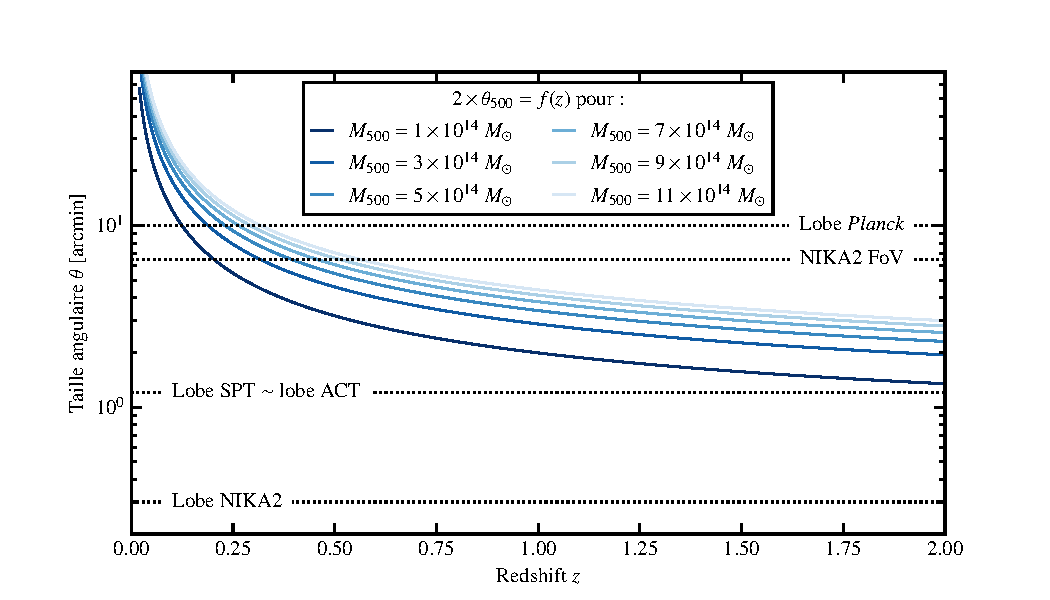
\includegraphics[width=.85\linewidth]{Figures/chap_nk/angular_sizes.pdf}
    \caption{
        Évolution du diamètre angulaire caractéristique $2\theta_{500}$ d'amas de galaxies de différentes masses avec le redshift.
        Les lobes de NIKA2 ($\sim 18$'' à 150 GHz), SPT ($\sim 1.2$'), ACT ($\sim 1.4$'), et \textit{Planck} ($\sim 10$') sont représentés à titre indicatif, de même que le champ de vue instantané (FoV pour \textit{field of view}) de NIKA2 (6.5').
    }
    \label{fig:nk_angular_sizes}
\end{figure*}

La résolution d'amas de galaxies est cruciale pour l'étude de leurs propriétés physiques.
En effet, les observations réalisées par un instrument fournissent une image du ciel convoluée par son lobe.
Par conséquent, la carte d'un amas de galaxies plus petit que la résolution de l'instrument qui l'observe est principalement une carte du lobe de l'instrument, qui ne permet pas une étude détaillée de la structure de l'amas.
C'est pourquoi les cartes de l'effet SZ construites par la collaboration \textit{Planck} \cite{planck_collaboration_planck_2016}, de résolution angulaire $\sim 10$', permettent seulement l'étude détaillée d'amas proches et massifs (comme l'amas de Coma, $z = 0.023, \, M_{500} \simeq 7 \times 10^{14} \;M_\odot$ \cite{ade_planck_2013}).

De la même façon, résoudre un amas (c'est-à-dire l'observer avec un lobe plus petit que son rayon caractéristique) ne permet pas nécessairement un grand niveau de détail dans l'extraction de ses propriétés physiques.
Pour des études précises, il est donc nécessaire que la taille angulaire de l'amas soit non seulement supérieure à la taille du lobe de l'instrument utilisé, mais aussi grande devant celle-ci.
C'est pourquoi les instruments ayant une résolution de l'ordre de la minute d'arc, comme SPT et ACT, ne permettent pas l'étude détaillée d'amas distants: au delà d'un redshift de 0.5, les tailles d'amas $2\theta_{500}$ ne sont au maximum que cinq fois plus grands que les lobes de ces instruments.
La cartographie détaillée de l'effet SZ dans les amas de galaxies nécessite donc l'utilisation d'un instrument à plus haute résolution angulaire.
Comme le montre la figure \ref{fig:nk_angular_sizes}, le lobe de NIKA2 à 150 GHz est inférieur par au moins un ordre de grandeur au diamètre angulaire $2\theta_{500}$ de tous les amas de masse $M_{500} > 3 \times 10^{14} \;M_\odot$, quel que soit leur redshift.
NIKA2 est donc un instrument idéal pour les observations SZ à haute résolution des amas de galaxies distants de l'Univers.

\subsubsection{Grande sensibilité} % -------------------------------------------------- %
La cartographie de l'effet SZ en direction d'amas de galaxies requiert une grande sensibilité.
En effet, la distorsion spectrale due à l'effet SZ est faible.
Dans le cas d'observations avec NIKA2 à 150 GHz, la brillance de surface maximale en direction des amas est de l'ordre du mJy/beam; à titre comparatif, la densité de flux d'Uranus à cette fréquence est de l'ordre de la dizaine de Jy/beam, de même que les fluctuations du bruit de l'atmosphère (ce point sera traité au chapitre suivant).
Par conséquent, une grande sensibilité est nécessaire à la mesure de l'effet SZ dans un temps raisonnable.
NIKA2 est capable de cartographier environ 1400 arcmin$^2$ avec un niveau de bruit de 1 mJy en une heure, ce qui permet d'atteindre le niveau de bruit requis pour la détection de l'effet SZ rapidement, comme discuté dans l'équation (\ref{eq:nk_time}).

\vspace{20pt}

Ainsi, les caractéristiques instrumentales de NIKA2 en font un instrument de choix pour étudier avec un grand niveau de détail les amas de galaxies lointains, non-résolus par \textit{Planck} et difficilement par SPT ou ACT.

% ------------------------------------------------------------------------------------- %
\subsection{Échantillon du grand programme SZ}

Le temps alloué aux observations du LPSZ a été réparti sur un échantillon d'environ cinquante amas de galaxies.
Cet échantillon est l'une des grandes forces du programme: il couvre une grande gamme de masses ($M_{500} \in [3,\,11] \times 10^{14} \;M_\odot$) à haut redshift ($z \in [0.5,\,0.9]$), avec des amas sélectionnés dans des catalogues SZ.
Il est représenté en figure \ref{fig:lpsz_sample}.

Comme nous l'avons discuté au chapitre précédent (voir \ref{sec:sz}), les échantillons sélectionnés par effet SZ ont l'avantage d'être proches d'échantillons sélectionnés en masse.
En effet, le paramètre de Compton intégré étant lié au contenu en énergie thermique de l'amas, il est étroitement lié à la masse (voir section \ref{sec:scaling:sz}, page \pageref{sec:scaling:sz}).
Ainsi, un échantillon construit avec pour critère une valeur de $Y$ supérieure à un seuil choisi sélectionnera les amas sur un critère lié à leur masse, ce qui permet d'éviter de favoriser un type d'amas particulier.
Un tel échantillon est alors dit représentatif, puisque la distribution des propriétés physiques des amas le constituant suit \prior\ la même distribution que les amas de l'Univers dans la gamme de masse considérée.
À titre d'exemple, les amas sélectionnés selon leur pic de luminosité en X ne sont pas représentatifs: la brillance de surface X étant proportionnelle au carré de la densité d'électrons intégrée le long de la ligne de visée (équation \ref{eq:x_brightness}), une telle sélection favorise les amas à cœur dense, qui présentent la caractéristique générale d'être plus relaxés (voir discussion sur les amas à cœur froid en \ref{sec:lpsz_sci}).

La sélection de l'échantillon a donc été basée sur les catalogues SZ existant au début du programme, à savoir les catalogues \textit{Planck} et ACT \cite{planck_collaboration_planck_2016-2, hasselfield_atacama_2013}.
Les amas ont été choisis parmi ceux présents dans les catalogues et visibles depuis le télescope de 30 mètres de l'IRAM (cf. \ref{sec:30m_geo} et figure \ref{fig:30m_sky}), et de manière à couvrir la gamme de masse considérée de manière homogène.
Pour cela, dix \guillemotleft boites \guillemotright\ ont été définies, délimitant deux intervalles en redshift et cinq en masse.
Cinq amas ont été tirés au hasard pour remplir chacune de ces boites, dans le catalogue ACT pour les deux boites de basse masse, et dans le catalogue \textit{Planck} pour les autres.
Dans les deux cas, les estimateurs de masse utilisés pour la répartition sont calculés à partir du signal SZ intégré mesuré par les relevés en utilisant la relation d'échelle de \cite{arnaud_universal_2010}.
Sans cette procédure de division en boîtes du plan masse-redshift, les amas auraient été sélectionnés aléatoirement dans les catalogues \textit{Planck} et ACT, et leur distribution en masse et en redshift aurait suivi la fonction de masse sous-jacente.
À l'inverse, l'échantillon du grand programme SZ constitue une couverture homogène de la gamme de masse et de redshift considérée.
Nous verrons en \mypageref{sec:scaling:intercept_bias} l'impact de cette sélection sur l'ajustement de la relation d'échelle masse-observable à partir des données du grand programme SZ.

\begin{figure*}[t]
    \centering
    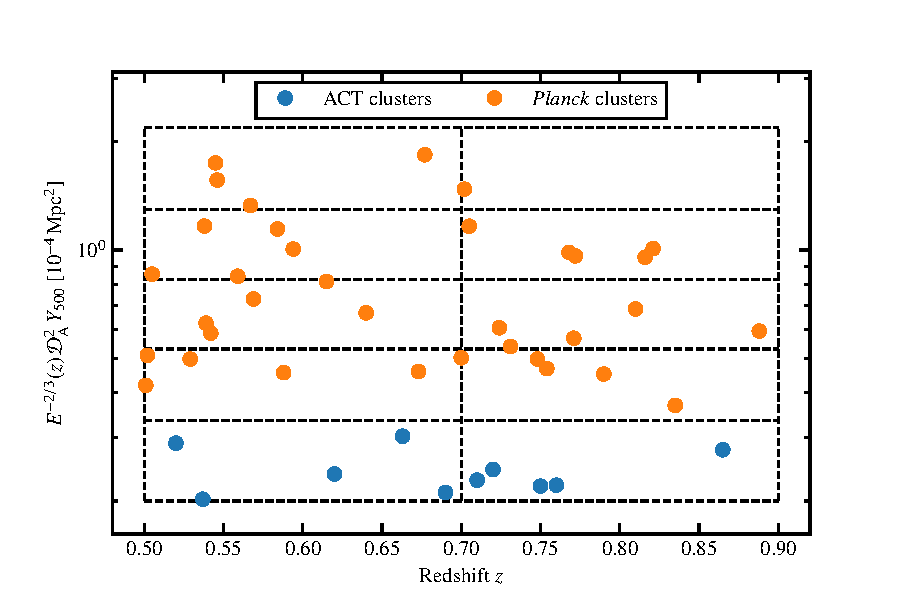
\includegraphics[width=.8\linewidth]{Figures/Chap_nk/lpsz_sample.pdf}
    \caption{
        Distribution des amas du grand programme SZ dans le plan redshift -- paramètre de Compton intégré.
        Les points bleu et orange représentent respectivement les amas extraits des catalogues ACT \cite{hasselfield_atacama_2013} et \textit{Planck} \cite{planck_collaboration_planck_2016-2}.
        Les lignes noires pointillées représentent les limites des boites utilisées pour construire l'échantillon.
    }
    \label{fig:lpsz_sample}
\end{figure*}

Le suivi SZ à haute résolution d'un échantillon d'amas aussi nombreux, à des redshifts supérieurs à 0.5, et sur une si grande gamme de masse est sans précédent.
Il permettra de comparer les propriétés d'amas de galaxies distants, mesurées en SZ avec une grande résolution angulaire, à celles mesurées sur des échantillons d'amas proches, mesurés en X ou en SZ avec une faible résolution.

Comme nous l'avons mentionné, le temps alloué au LPSZ est de 300 heures d'observation.
La distribution de ces heures entre les différents amas de l'échantillon a été calculée de façon à obtenir un signal de qualité équivalente pour chacun des amas.
Le temps alloué à un amas est ainsi calculé comme le temps d'observation nécessaire à l'obtention d'un rapport signal-sur-bruit du profil de brillance de surface SZ de $3\sigma$ au rayon caractéristique $R_{500}$.
Ce calcul est basé sur plusieurs hypothèses.
D'une part, il a été supposé que le profil de pression de chaque amas était donné par le profil de pression universel du milieu intra-amas d'\myciteauthor{arnaud_universal_2010}, discuté en \mypageref{sec:univ_press_prof}.
D'autre part, le calcul a été fait dans l'hypothèse où la masse $M_{500}$ des amas de l'échantillon était égale à celle donnée par les catalogues \textit{Planck} et ACT dans lesquels les amas sont choisis.
Celles-ci ont été obtenues par l'utilisation d'une relation d'échelle liant l'observable des relevés SZ à la masse.
À partir de ces deux hypothèses, un profil de paramètre de Compton a été calculé pour chaque amas.
Le temps d'observation en a été déduit en suivant le calcul présenté en équation (\ref{eq:nk_time}) comme le temps nécessaire pour atteindre un niveau de bruit trois fois inférieur à la valeur de ce profil à $R_{500}$.
On note que tout écart aux hypothèses émises au cours de ce calcul, par exemple sur le profil de pression du milieu intra-amas ou sur la relation d'échelle masse-observable, entraine un changement dans la qualité du signal attendu.
Ainsi, un amas dont la masse est mal estimée par la relation d'échelle, ou dont le profil de pression présente un écart au profil universel, peut présenter une qualité de données significativement différente de celle attendue.
De plus, les temps d'observation ont été calculés avant la construction de NIKA2, et les performances réelles de l'instrument étaient encore inconnues.
Par conséquent, il est possible que la qualité générale des observations NIKA2 des amas de l'échantillon soient moins bonne qu'attendu.
Ce point nécessite une grande précaution, car pour étalonner les outils nécessaires à la cosmologie, l'échantillon doit être représentatif, et les observations des amas doivent avoir une qualité équivalente afin de ne pas donner un poids trop important à un type d'amas donné.

% ------------------------------------------------------------------------------------- %
\subsection{Objectifs scientifiques du grand programme SZ} \label{sec:lpsz_sci}

Le grand programme SZ exploite les performances de NIKA2 et sa capacité à mesurer l'effet SZ à haute résolution dans le but de répondre à plusieurs questions de la cosmologie avec des amas de galaxies.

\subsubsection{Études détaillées des amas de l'échantillon} % -------------------------- %
Comme discuté en section \ref{sec:nk_sz}, les performances et caractéristiques de NIKA2 sont en adéquation avec les besoins pour l'étude à haute résolution d'amas de galaxies.
Par conséquent, les observations des amas du LPSZ avec NIKA2 permettent de les imager avec un grand niveau de détail.
Les études des propriétés individuelles de chaque amas sont alors rendues possibles.

Les résultats de ces études seront rendus disponibles par la collaboration NIKA2 à la fin du programme.
Certaines études individuelles le sont déjà, notamment les deux premières études individuelles du LPSZ: \cite{ruppin_first_2018}, et \cite{keruzore_exploiting_2020}, menée au cours de cette thèse et présentée au chapitre \ref{chap:actj0215}.
Les produits finaux seront pour chacun des amas de l'échantillon du LPSZ:
\begin{itemize}[leftmargin=*]
\setlength\itemsep{5pt}
    \item Les cartes NIKA2 de la région de l'amas, à 150 et 260 GHz, étalonnées et soustraites du bruit corrélé (voir chapitre \ref{chap:decorr});
    \item Le profil de pression de l'amas mesuré avec le logiciel \texttt{PANCO2}, développé dans le cadre de cette thèse, et présenté au chapitre \ref{chap:panco};
    \item Les valeurs des grandeurs caractéristiques intégrées de l'amas, $R_{500}$, $Y_{500}$, et $M_{500}$, qui pourront être utilisées par la communauté pour améliorer la mesure de la relation d'échelle masse-observable dans les analyses cosmologiques de catalogues d'amas de galaxies -- voir section \ref{sec:scaling}, et chapitre \ref{chap:scaling}.
\end{itemize}
Toutes ces informations seront rendues publiques sous la forme d'un catalogue, et utilisables par la communauté pour combiner les informations issues de l'analyse des amas du LPSZ avec d'autres données futures, afin d'enrichir la connaissance de la physique des amas de galaxies grâce à l'échantillon du LPSZ.

\subsubsection{Profil de pression moyen des amas de galaxies} % ----------------------- %
L'un des objectifs principaux du LPSZ est la mesure du profil de pression moyen d'amas de galaxies à haut redshift.
Le profil universel d'\myciteauthor{arnaud_universal_2010}, obtenu par l'exploitation de l'échantillon REXCESS en X à $z < 0.2$, a été utilisé dans la construction de plusieurs catalogues d'amas en SZ, notamment par les collaborations ACT \cite{hilton_atacama_2021} et \textit{Planck} \cite{planck_collaboration_planck_2016-2}.
Il est intéressant de noter que dans les deux cas, les catalogues sont construits à partir de détections des amas par effet SZ, et qu'ils comportent des amas à des redshifts bien plus grands que 0.2, redshift maximal du suivi REXCESS.
Deux questions se posent alors:
\begin{itemize}[leftmargin=*]
\setlength\itemsep{5pt}
\item
    Le profil de pression moyen des amas pourrait-il être différent de la mesure d'\citeauthor{arnaud_universal_2010}? \\
    Une différence pourrait avoir plusieurs origines.
    D'une part, les mesures de profil de pression en X requièrent l'estimation de la température du milieu intra-amas par spectroscopie, qui présente plusieurs incertitudes systématiques complexes \cite{bohringer_x-ray_2010}.
    Il est donc possible que les profils de pression mesurés en X et en SZ ne soient pas strictement équivalents.
    D'autre part, le profil de pression moyen des amas pourrait évoluer avec le redshift.
    Dans ce cas, l'utilisation d'un profil de pression évalué à $z < 0.2$ serait inadaptée à la détection d'amas aussi lointains que $z=2$ (dans le cas du relevé ACT), ou même jusqu'à $z=1$ (dans le cas de \textit{Planck}).
    Enfin, ce profil de pression pourrait ne pas être représentatif de tous les amas de l'Univers, à cause des effets de sélection caractéristiques des échantillons d'amas détectés en X discutés précédemment.
\item
Quel impact aurait une variation du profil de pression moyen sur les analyses cosmologiques basées sur l'effet SZ? \\
    Comme nous l'avons vu, la connaissance du profil de pression moyen des amas est nécessaire à l'extraction de catalogues d'amas à partir d'observations millimétriques.
    Une variation du profil -- avec la méthode de détection ou avec le redshift -- pourrait ainsi \prior\ modifier les catalogues issus des cartes de \textit{Planck} et ACT, et donc les résultats des mesures de paramètres cosmologiques.
    Cet impact a été quantifié dans le cas d'analyses du spectre de puissance de l'effet SZ par \myciteauthor{ruppin_impact_2019}, en analysant la carte de paramètre de Compton issue des données de \textit{Planck} \cite{planck_collaboration_planck_2016} avec différents profils de pression moyens.
    Leurs résultats montrent qu'une modification de l'amplitude du profil de pression aussi faible que 15\% peut affecter significativement les résultats des analyses cosmologiques.
\end{itemize}

L'objectif du LPSZ est de répondre à ces questions en mesurant le profil de pression moyen des amas de son échantillon.
Plusieurs études récentes s'intéressent à de possibles variations du profil de pression moyen des amas avec le redshift, mais utilisent principalement des observations X (\eg\ \cite{mcdonald_redshift_2014, ghirardini_evolution_2021}).
L'utilisation de données SZ à haute résolution offrira des contraintes complémentaires, et créera l'opportunité de comparaisons de résultats multilongueur d'onde.

\subsubsection{Combinaisons multilongueur d'onde et propriétés thermodynamiques} % -- %
Comme nous l'avons vu au chapitre précédent, les observations de l'effet tSZ permettent de sonder la pression thermique des électrons du milieu intra-amas.
Si celle-ci donne des informations importantes sur les amas, d'autres propriétés thermodynamiques revêtent également une grande importance pour l'étude de la physique de ces objets, et ne sont pas mesurables par l'effet tSZ seul.

C'est la raison pour laquelle le LPSZ comporte un suivi de tous ses amas à d'autres longueurs d'onde, complémentaires à l'effet SZ.
Un suivi en X avec les satellites \textit{XMM-Newton} et \textit{Chandra} est notamment l'un des grands points forts du programme.
La combinaison de ces observations avec celles effectuées avec NIKA2 permettra la première étude des propriétés thermodynamiques d'un échantillon d'amas à $z > 0.5$ avec des données X et SZ de qualité comparable.
En effet, comme détaillé en section \mypageref{sec:cluster_obs}, les observations X et SZ sont très complémentaires, puisqu'elles sondent respectivement la densité et la pression du milieu intra-amas qui peuvent être combinées pour calculer la masse de l'amas.
Mais d'autres propriétés peuvent également être calculées par cette combinaison.
Par exemple, le profil de température du milieu intra-amas, dans l'hypothèse d'un gaz parfait, s'écrit:
\begin{equation}
    \label{eq:temperature}
    k_\textsc{b}T_\e(r) = P_\e(r) / n_\e(r),
\end{equation}
et permet d'étudier l'état dynamique de l'amas, pouvant révéler des mécanismes de fusion de plusieurs sous-amas (\eg\ \cite{adam_mapping_2017,ruppin_unveiling_2020}).
Les mesures de température permettent également l'étude des corrections relativistes à l'effet SZ, qui dépendent de cette dernière, comme décrit en section \mypageref{sec:sz}.
On peut également définir le paramètre d'entropie, introduit par \myciteauthor{voit_modified_2002} comme:
\begin{equation}
    \label{eq:entropy}
    K_\e(r) = P_\e(r) \, n_\e(r)^{-5/3}.
\end{equation}
Cette quantité, souvent nommée entropie du milieu intra-amas, est liée au caractère adiabatique de l'évolution de l'amas; dans l'hypothèse où le milieu intra-amas est un gaz parfait monoatomique d'électrons, on peut écrire la loi de Laplace $PV^\gamma = {\rm cste}$ comme:
\begin{equation}
    P_\e \, n_\e^{-5/3} = {\rm cste},
\end{equation}
et la combinaison avec l'équation (\ref{eq:entropy}) permet d'identifier $K_\e$ comme le terme constant.
Ce paramètre d'entropie est donc intimement lié à l'entropie thermodynamique du milieu intra-amas: la formule de de Sackur-Tetrode donne l'entropie par particule d'un gaz parfait $s$, qui peut s'exprimer en fonction de $K_\e$ comme:
\begin{equation}
    \label{eq:entropy_s_K}
    s = k_\textsc{b} \ln K_\e^{3/2} + {\rm cste}.
\end{equation}
Le paramètre $K_\e$ peut donc être interprété comme une mesure en échelle exponentielle de l'entropie par particule $s$, ou encore comme une mesure du nombre d'états microscopiques $\Omega$ par comparaison de l'équation (\ref{eq:entropy_s_K}) et de l'équation de Boltzmann, $S = k_\textsc{b} \ln \Omega$.

Le paramètre d'entropie, simplement nommé entropie dans la suite, est d'un intérêt considérable pour l'étude de la physique des amas (voir \cite{voit_tracing_2005} -- en particulier la section IV -- pour une revue).
Il a historiquement été étudié dans des simulations d'amas de galaxies.
Dans le cas où seuls les processus gravitationnels sont considérés pour la formation des amas, l'entropie dans les amas croît en loi de puissance avec le rayon.
Ce comportement est observé dans les simulations à $N$ corps considérant des particules de matière sombre seulement, donnant des profils d'entropie de forme $K_\e(r) \propto r^{1.1}$ \cite{voit_tracing_2005}.
Dans les simulations plus complexes, de même que dans les amas réels, on observe un écart à ce comportement, en particulier dans le cœur des amas.
Cet écart est dû aux phénomènes tels que des fusions de sous-structures, ou encore l'injection d'énergie par des noyaux actifs de galaxies ou des explosions de supernovas, principalement localisés dans le cœur des amas, et qui augmentent l'entropie du gaz.
Il est illustré en figure \ref{fig:entropy_rexcess} pour l'échantillon REXCESS, discuté précédemment.
On voit que le profil d'entropie des amas suit bien $K_\e(r) \propto r^{1.1}$ à grand rayon, mais que le centre des profils montre un écart significatif.
Cet écart est d'autant plus fort que le cœur des amas est perturbé: les profils bleus, correspondant aux amas \textit{cool-core}, sont plus en accord avec $K_\e(r) \propto r^{1.1}$ que les courbes rouges, correspondant aux amas perturbés.
L'entropie $K_\e$ représente donc un traceur de l'histoire thermique du milieu intra-amas, son écart au profil d'entropie purement gravitationnel donnant une forme de mémoire des processus non-gravitationnels ayant eu lieu au sein des amas.

\begin{figure*}[t]
    \centering
    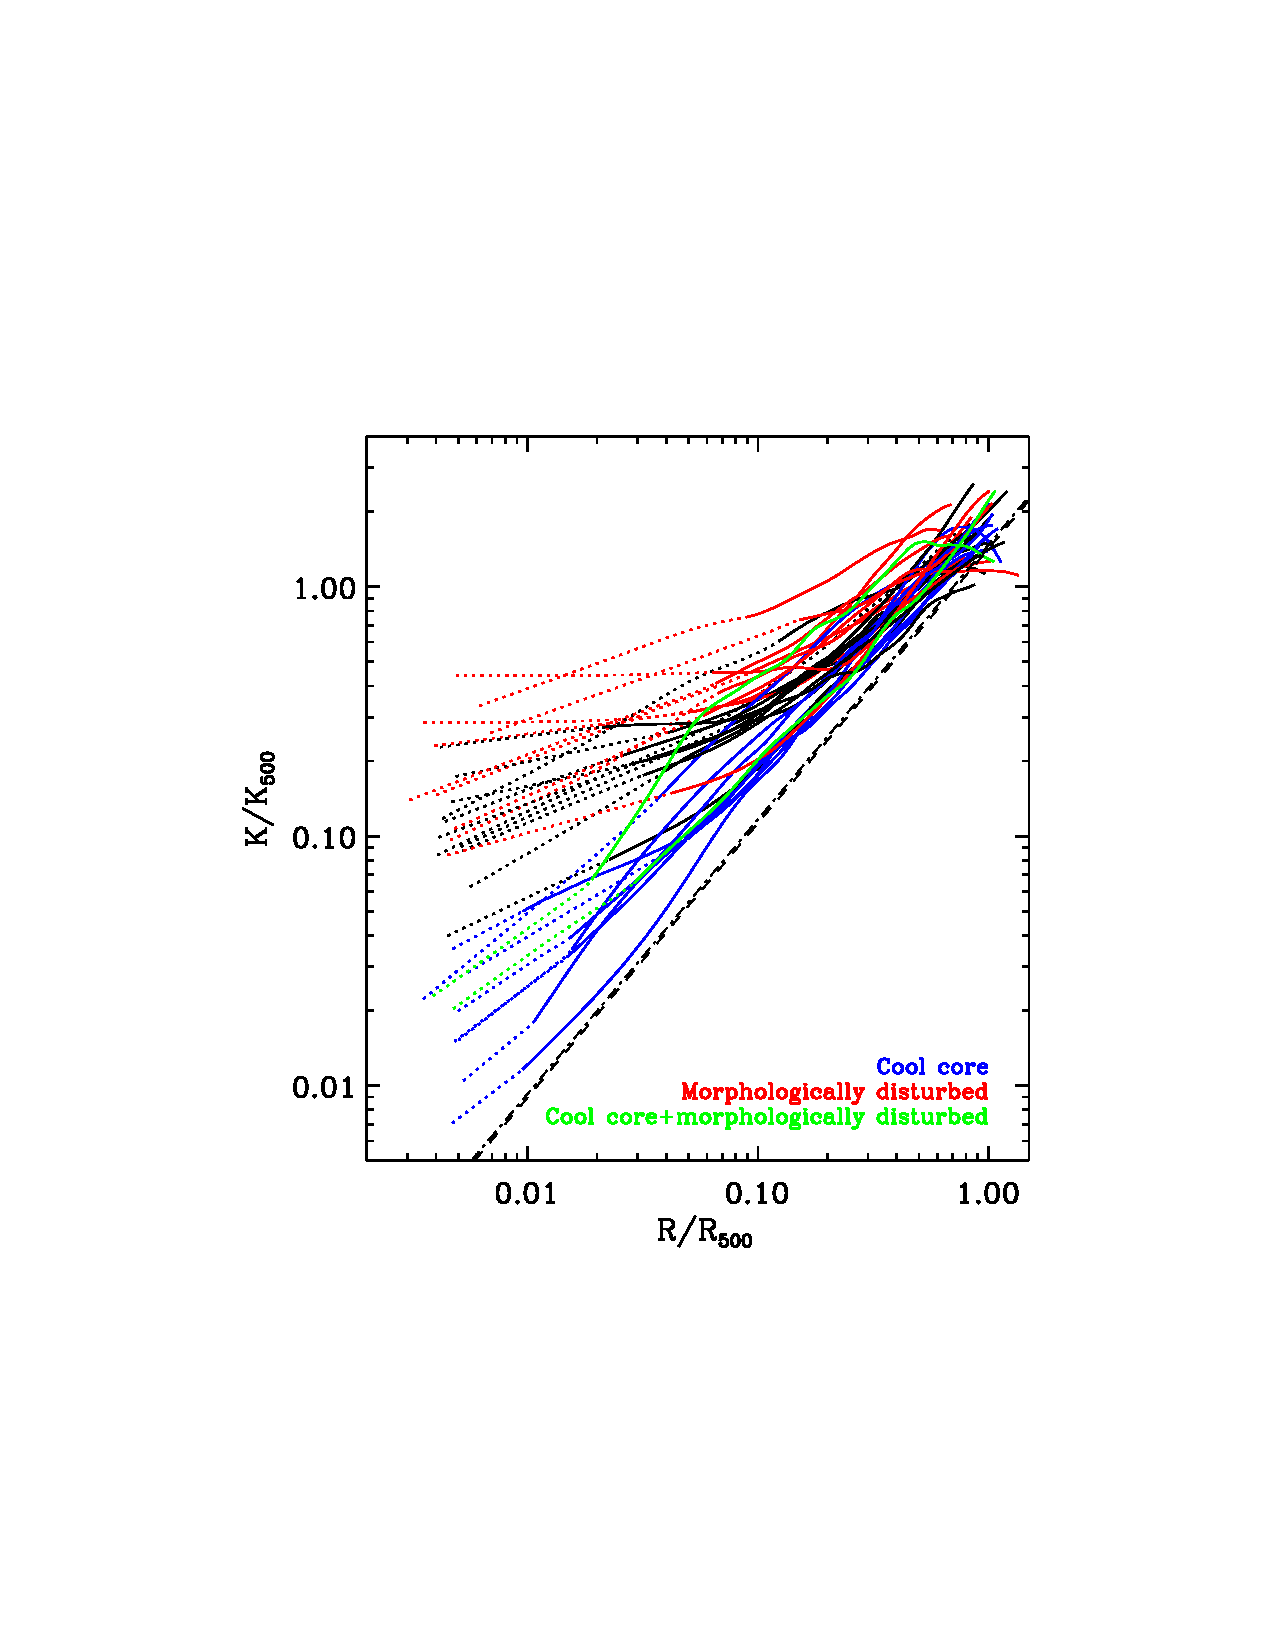
\includegraphics[width=.6\linewidth]{Figures/Chap_nk/entropy_pratt.pdf}
    \caption{
        Profils d'entropie mesurés à partir des observations \textit{XMM-Newton} des amas de l'échantillon REXCESS.
        Les lignes pointillées noires marquent le profil en $r^{1.1}$ attendu pour une formation d'amas purement par effondrement gravitationnel.
        Les courbes bleues et rouges sont respectivement les profils d'amas classifiés comme \textit{cool-core} et à cœur perturbé.
        Figure extraite de \cite{pratt_gas_2010}.
    }
    \label{fig:entropy_rexcess}
\end{figure*}

Les combinaisons de mesures X et SZ permettront donc au LPSZ d'étudier en détail les propriétés thermodynamiques du milieu intra-amas jusqu'à un redshift de $0.9$, pour un échantillon d'amas sélectionnés en SZ.
Outre leur importance directe pour la physique des amas, ces mesures pourront être utilisées pour classer les amas en fonction de leurs propriétés dynamiques.
En particulier, on trouve dans l'Univers des amas à cœur froid (ou \textit{cool core}), dont les propriétés centrales indique un état de relaxation, et les amas au cœur perturbé.
Ces deux types d'amas ont des propriétés globalement différentes, comme décrit par exemple dans l'étude de \myciteauthor{hudson_what_2010}, qui étudie les différences entre les amas \textit{cool-core} et perturbés sur le critère de 16 propriétés physiques différentes.
En outre, les amas à cœur froid possèdent une entropie centrale bien plus faible que les amas perturbés, caractéristique d'injections d'énergie non-thermiques moins importantes.
Ils ont également une densité centrale plus élevée (et sont ainsi plus facilement détectés en X), ainsi qu'un profil de pression bien plus piqué en leur centre.
Nous avons discuté de l'importance de la mesure du profil de pression moyen des amas de galaxies pour les études cosmologiques; une différence significative entre deux populations d'amas pourrait également avoir un impact sur de telles études.
Les observations du LPSZ, en étudiant la température, l'entropie, et la pression du milieu intra-amas à l'aide d'observations résolues en X et en SZ, pourront distinguer ces populations, et les étudier séparément pour approfondir la connaissance de leurs propriétés thermodynamiques et de leur distribution dans les différentes populations.

De plus, comme nous l'avons discuté au chapitre précédent, les observations SZ permettent de réduire le temps nécessaire par rapport aux observations X permettant les mesures spectroscopiques.
Traditionnellement, les études résolues d'amas faisaient appel à des observations X profondes, afin de pouvoir extraire un profil de température par spectroscopie, et ainsi de pouvoir déduire une mesure du profil de pression.
Avec un profil de pression fourni par les mesures en SZ, la spectroscopie X n'est plus nécessaire pour remonter à la masse.
Toutefois, certains des amas du LPSZ ont été suivis en X avec des observations profondes, permettant les études spectroscopiques.
Pour de telles observations, la combinaison des observations SZ et X (sans spectroscopie) pourra être comparée aux mesures X seules, pour étudier de potentielles différences pouvant être dues aux incertitudes systématiques affectant les mesures de température en spectroscopie X (voir \cite{bohringer_x-ray_2010} pour une revue).

Enfin, des suivis en optique sont également en cours pour les amas du LPSZ, avec le Gran Telescopio Canarias à l'observatoire des Canaries.
Ce suivi spectroscopique permettra d'étudier la distribution des galaxies des amas du LPSZ, ainsi que leurs masses par dispersion des vitesses (voir par exemple \cite{barrena_optical_2020} pour une étude similaire de suivi des amas \textit{Planck} avec le Gran Telescopio Canarias).
De plus, certains des amas du LPSZ font partie d'échantillons d'amas suivis par d'autres instruments; par exemple, l'échantillon CLASH \cite{postman_cluster_2012}, ayant réalisé un suivi d'amas avec le \textit{Hubble Space Telescope} dont les données sont aujourd'hui publiques.
Ces données permettront des études de la masse d'amas du LPSZ par des mesures optiques, en utilisant la dispersion des vitesses pour le suivi spectroscopique et le lentillage gravitationnel pour les données de HST.
Ces estimateurs de masses, comme nous l'avons discuté en \mypageref{sec:cluster_obs}, ne sont pas affectés par le biais hydrostatique, mais peuvent souffrir de biais différents \cite{becker_accuracy_2011, grandis_calibration_2021}.
La comparaison des mesures de masse dans ces suivis avec celles obtenues par combinaison des observations SZ avec NIKA2 et X permettra donc d'étudier ce biais pour une partie de l'échantillon \cite{munoz_echevarria_lpsz-clash_2021}.

\subsubsection{La relation d'échelle} % ----------------------------------------------- %
Comme nous l'avons vu en \ref{sec:scaling}, la connaissance du lien entre la masse d'un amas et son observable dans un relevé est cruciale pour l'exploitation cosmologique du relevé en question.
Tout comme pour le profil de pression moyen du milieu intra-amas, l'étude de ce lien a aujourd'hui principalement été menée en utilisant des amas proches, et des masses souvent mesurées à l'aide uniquement d'observations X (\eg\ \cite{arnaud_universal_2010,planck_collaboration_planck_2011}).
Les mêmes questions se posent alors, interrogeant sur de possibles variations de la relation avec le redshift, avec l'utilisation de données SZ, et sur l'impact de telles variations sur les résultats cosmologiques.

Afin de pouvoir utiliser l'échantillon du LPSZ pour étudier de possibles évolutions de la relation d'échelle, il est nécessaire de connaître la masse des amas.
Comme nous l'avons vu en \ref{sec:sz}, l'effet SZ seul ne permet pas de mesurer la masse d'un amas.
Celle-ci peut cependant être estimée à partir de la combinaison d'observations SZ et X, comme discuté en \ref{sec:x}.
La mesure de la relation d'échelle fera donc appel à la combinaisons des observations SZ et X des amas de l'échantillon détaillée précédemment.
En plus des mesures de masse, l'étude des propriétés thermodynamiques des amas et leur classification basée sur ces propriétés permettra des études systématiques détaillées sur l'impact des propriétés des amas sur la relation d'échelle.
Par exemple, les amas perturbés pourraient suivre une relation d'échelle différente de celle suivie par les amas à cœur froid.
Une étude intéressante serait la réduction de la dispersion autour de la relation d'échelle grâce aux propriétés thermodynamiques des amas, mesurées en détail à l'aide de la combinaison des observations avec NIKA2 et \textit{XMM-Newton} ou \textit{Chandra}.
Jusqu'à présent, les relations d'échelles sont mesurées en supposant des relations en loi de puissance avec une dispersion intrinsèque, comme décrit en section \mypageref{sec:scaling} et au chapitre \ref{chap:scaling}.
Une autre approche pourrait être la réduction de cette dispersion basée sur des propriétés observables des amas.
De telles études sont menées pour mesurer les paramètres cosmologiques à l'aide des supernovas de type Ia, par exemple avec le modèle SALT2 (\cite{guy_salt2_2007}).
Dans de tels travaux (\eg\ \cite{betoule_improved_2014}), le module de distances de chacune des supernovas est corrigé à partir de propriétés observables de l'objet, permettant de réduire la dispersion autour du diagramme de Hubble.
On parle alors des supernovas comme de chandelles standardisables, dont l'exploitation cosmologique repose sur une correction empirique basée sur la mesure des propriétés de chacun des objets.
Des études similaires pourraient être réalisées avec les amas du grand programme SZ, grâce à des observables des amas telles que leurs propriétés thermodynamiques, pour une approche différente à la mesure de relations d'échelle.

Comme nous l'avons mentionné au chapitre précédent, la mesure de relations d'échelle fait intervenir beaucoup d'effets systématiques, tels que les effets de sélection dus au choix des amas de l'échantillon.
Ces effets peuvent être pris en compte au prix d'une modélisation statistique complexe.
L'étude de la relation d'échelle liant la masse au paramètre de Compton intégré au chapitre \ref{chap:scaling}, en utilisant des simulations pour évaluer les différents effets systématiques affectant la mesure de cette relation dans le cadre du LPSZ.

% ===================================================================================== %
\section{La base de données du grand programme SZ de NIKA2}
\label{sec:nk_ami}

% ------------------------------------------------------------------------------------- %
\subsection{Contexte}

Avec l'avancement du grand programme SZ de NIKA2, la quantité d'informations pertinentes pour le programme a augmenté rapidement.
Il a donc été nécessaire de mettre en place un moyen permettant de centraliser ces informations, comportant des renseignements sur les observations NIKA2 ou sur l'existence de données externes.
Un exemple est le besoin d'avoir accès aux coordonnées les plus récentes d'un amas.
En effet, les amas du grand programme SZ sont en majorité issus du catalogue \textit{Planck} \cite{planck_collaboration_planck_2016-2}, construit à partir d'observations dont la résolution est proche de la taille du champ de vue de NIKA2.
Les coordonnées des amas dans ce catalogue sont donc imprécises; en observant à ces coordonnées avec NIKA2, il est possible d'observer à côté de l'amas.
Il est donc préférable d'utiliser les coordonnées d'amas obtenues avec des suivis à plus haute résolution, par exemple en X.
Il est donc important de pouvoir accéder aux coordonnées d'un amas les plus précises possibles.
Un autre exemple d'utilisation est la possibilité d'avoir un outil permettant de connaître rapidement le nombre de \textit{scans} ayant été effectués sur chaque amas, qui peut grandement faciliter la prise de décision sur la liste de sources choisies pour être observées au télescope.
De même, savoir si la collaboration dispose de données X ou optiques associées à un amas permet de choisir les sources considérées pour une analyse multilongueur d'onde.
Enfin, en sauvegardant les résultats des analyses de manière centralisée et accessible, la collaboration pourrait plus facilement garder une traçabilité de l'évolution des résultats avec les développements de logiciels de traitement des données, et choisir des amas de caractéristiques similaires pour une étude d'échantillon.

Il a donc été décidé de construire une base de données du grand programme SZ.
Dans ce contexte, nous avons choisi de collaborer avec les développeurs de AMI (\textit{Atlas Metadata Interface}, \cite{albrand_atlas_2010}), membres du service informatique du Laboratoire de Physique Subatomique et de Cosmologie.
AMI propose un cadre permettant de développer une base de métadonnées, c'est-à-dire un regroupement d'informations sous forme de texte (les données de NIKA2 ou d'autres instruments ne sont pas centralisées).
J'ai été nommé responsable scientifique de cette base de données, et ai pu collaborer avec les développeurs pour établir un cahier des charges, visant à concilier les besoins scientifiques et les possibilités offertes par AMI.

% ------------------------------------------------------------------------------------- %
\subsection{Contenu et interface de la base de données}

Le cahier des charges défini pour la base de données comprend plusieurs exigences.
D'une part, sa structure doit être assez souple pour stocker de l'information évoluant avec le temps, comme les coordonnées les plus précises existant pour chaque amas, l'existence de données externes, etc.
D'autre part, la base de données doit pouvoir être utilisée à plusieurs étapes de la chaîne d'analyse du grand programme SZ:
\begin{itemize}[leftmargin=*]
\setlength\itemsep{0pt}
\item Pendant les observations au télescope, pour accéder aux coordonnées des amas, au temps d'observation nécessaire et déjà effectué, etc.
\item Pendant l'analyse des données brutes, pour accéder à la liste des \textit{scans} associés à un amas et à leurs propriétés.
\item Pendant l'analyse des propriétés physiques des amas, pour accéder aux produits de l'analyse des données brutes (cartes SZ, etc.), aux propriétés des amas (redshift, masse estimée par \textit{Planck}).
\end{itemize}
Chacune des étapes est associée à des besoins d'interactivité différents: une table avec interface graphique est utile pendant les observations et pour avoir des informations rapides sur les amas, mais un accès par ligne de commande peut être plus utile pour l'interface avec les logiciels d'analyse.

La base de données AMI-LPSZ est accessible sur demande pour les membres de la collaboration NIKA2\footnote{\url{https://ami-nika2-lpsz.in2p3.fr/}}.
Elle est composée de plusieurs tables, correspondant chacune à un type de données, et interconnectées.
Les principales sont les suivantes:
\begin{itemize}[leftmargin=*]
\setlength\itemsep{0pt}
\item Une table \texttt{CLUSTER}, dont chaque élément est un amas.
    Les données stockées incluent le nom de chaque amas, ses coordonnées mesurées à partir de différents jeux de données (SZ, optique, X), sa masse et son redshift, le nombre de \textit{scans} à réaliser pour compléter les observations de l'amas, etc.
    Un champ est également présent pour stocker l'information sur l'existence de données externes, par exemple X avec \textit{Chandra} ou \textit{XMM-Newton}, ou submillimétrique pour la contamination par des sources ponctuelles (voir section \ref{sec:decor:pstools}).
\item une table \texttt{SCAN} qui regroupe chaque \textit{scan} effectué par la caméra NIKA2 depuis sa mise en service.
    Les informations associées à chaque \textit{scan} incluent la date et l'heure de l'observation, le nom de la source, le type de \textit{scan}, l'opacité atmosphérique et l'élévation, ou encore les commentaires laissés par les observateurs au moment de sa réalisation.
    J'ai été en charge de l'écriture du programme pour interroger la base de données de l'IRAM dans laquelle ces informations sont consignées pour pouvoir les inclure dans AMI.
    Pour les \textit{scans} dont le nom de source est l'un des amas de galaxies du grand programme SZ, un lien est créé entre le \textit{scan} et l'entrée correspondant à l'amas dans la table \texttt{CLUSTER}, de sorte à ce qu'il soit possible d'extraire la liste des \textit{scans} effectués pour chaque amas.
\item Une table \texttt{CAMPAIGN}, dont chaque élément est une campagne d'observation avec NIKA2.
    Chaque élément de la table \texttt{SCAN} est ainsi associé à une campagne d'observations.
    Cela permet de conserver des informations sur chaque campagne d'observations, comme une météo particulièrement capricieuse ou un problème dans l'acquisition des données, afin de pouvoir éventuellement exclure des \textit{scans} lors des analyses.
\item Une table \texttt{ANALYSIS}, qui répertorie les résultats d'analyse des amas individuels.
    La structure de cette table et son contenus sont toujours en cours de discussion.
    À terme, le but est de garder une trace des analyses des données brutes de NIKA2 (chapitre \ref{chap:decorr}) et des propriétés thermodynamiques (chapitre \ref{chap:panco}) dans AMI.
\end{itemize}

La base de données est accessible de deux façons.
D'une part, l'interface web offre une interface graphique qui permet de chercher des entrées dans les différentes tables.
Ces recherches peuvent être faites sur n'importe quel critère pouvant être construit à partir des différents champs présents dans les tables.
Deux exemples sont présentés en figure \ref{fig:ami_request}: une recherche des amas du programme dans l'intervalle de redshift $0.5 < z < 0.7$, et des \textit{scans} de l'amas \act\ effectués dans des conditions atmosphériques $0.1 < \tau_{225} < 0.2$.
Dans les deux cas, AMI permet d'extraire la liste des objets -- amas dans le premier cas, et \textit{scans} dans le second -- satisfaisant ces conditions, et leurs propriétés.
Chaque élément de la liste peut également être inspecté individuellement.

\begin{figure*}[t]
    \centering
    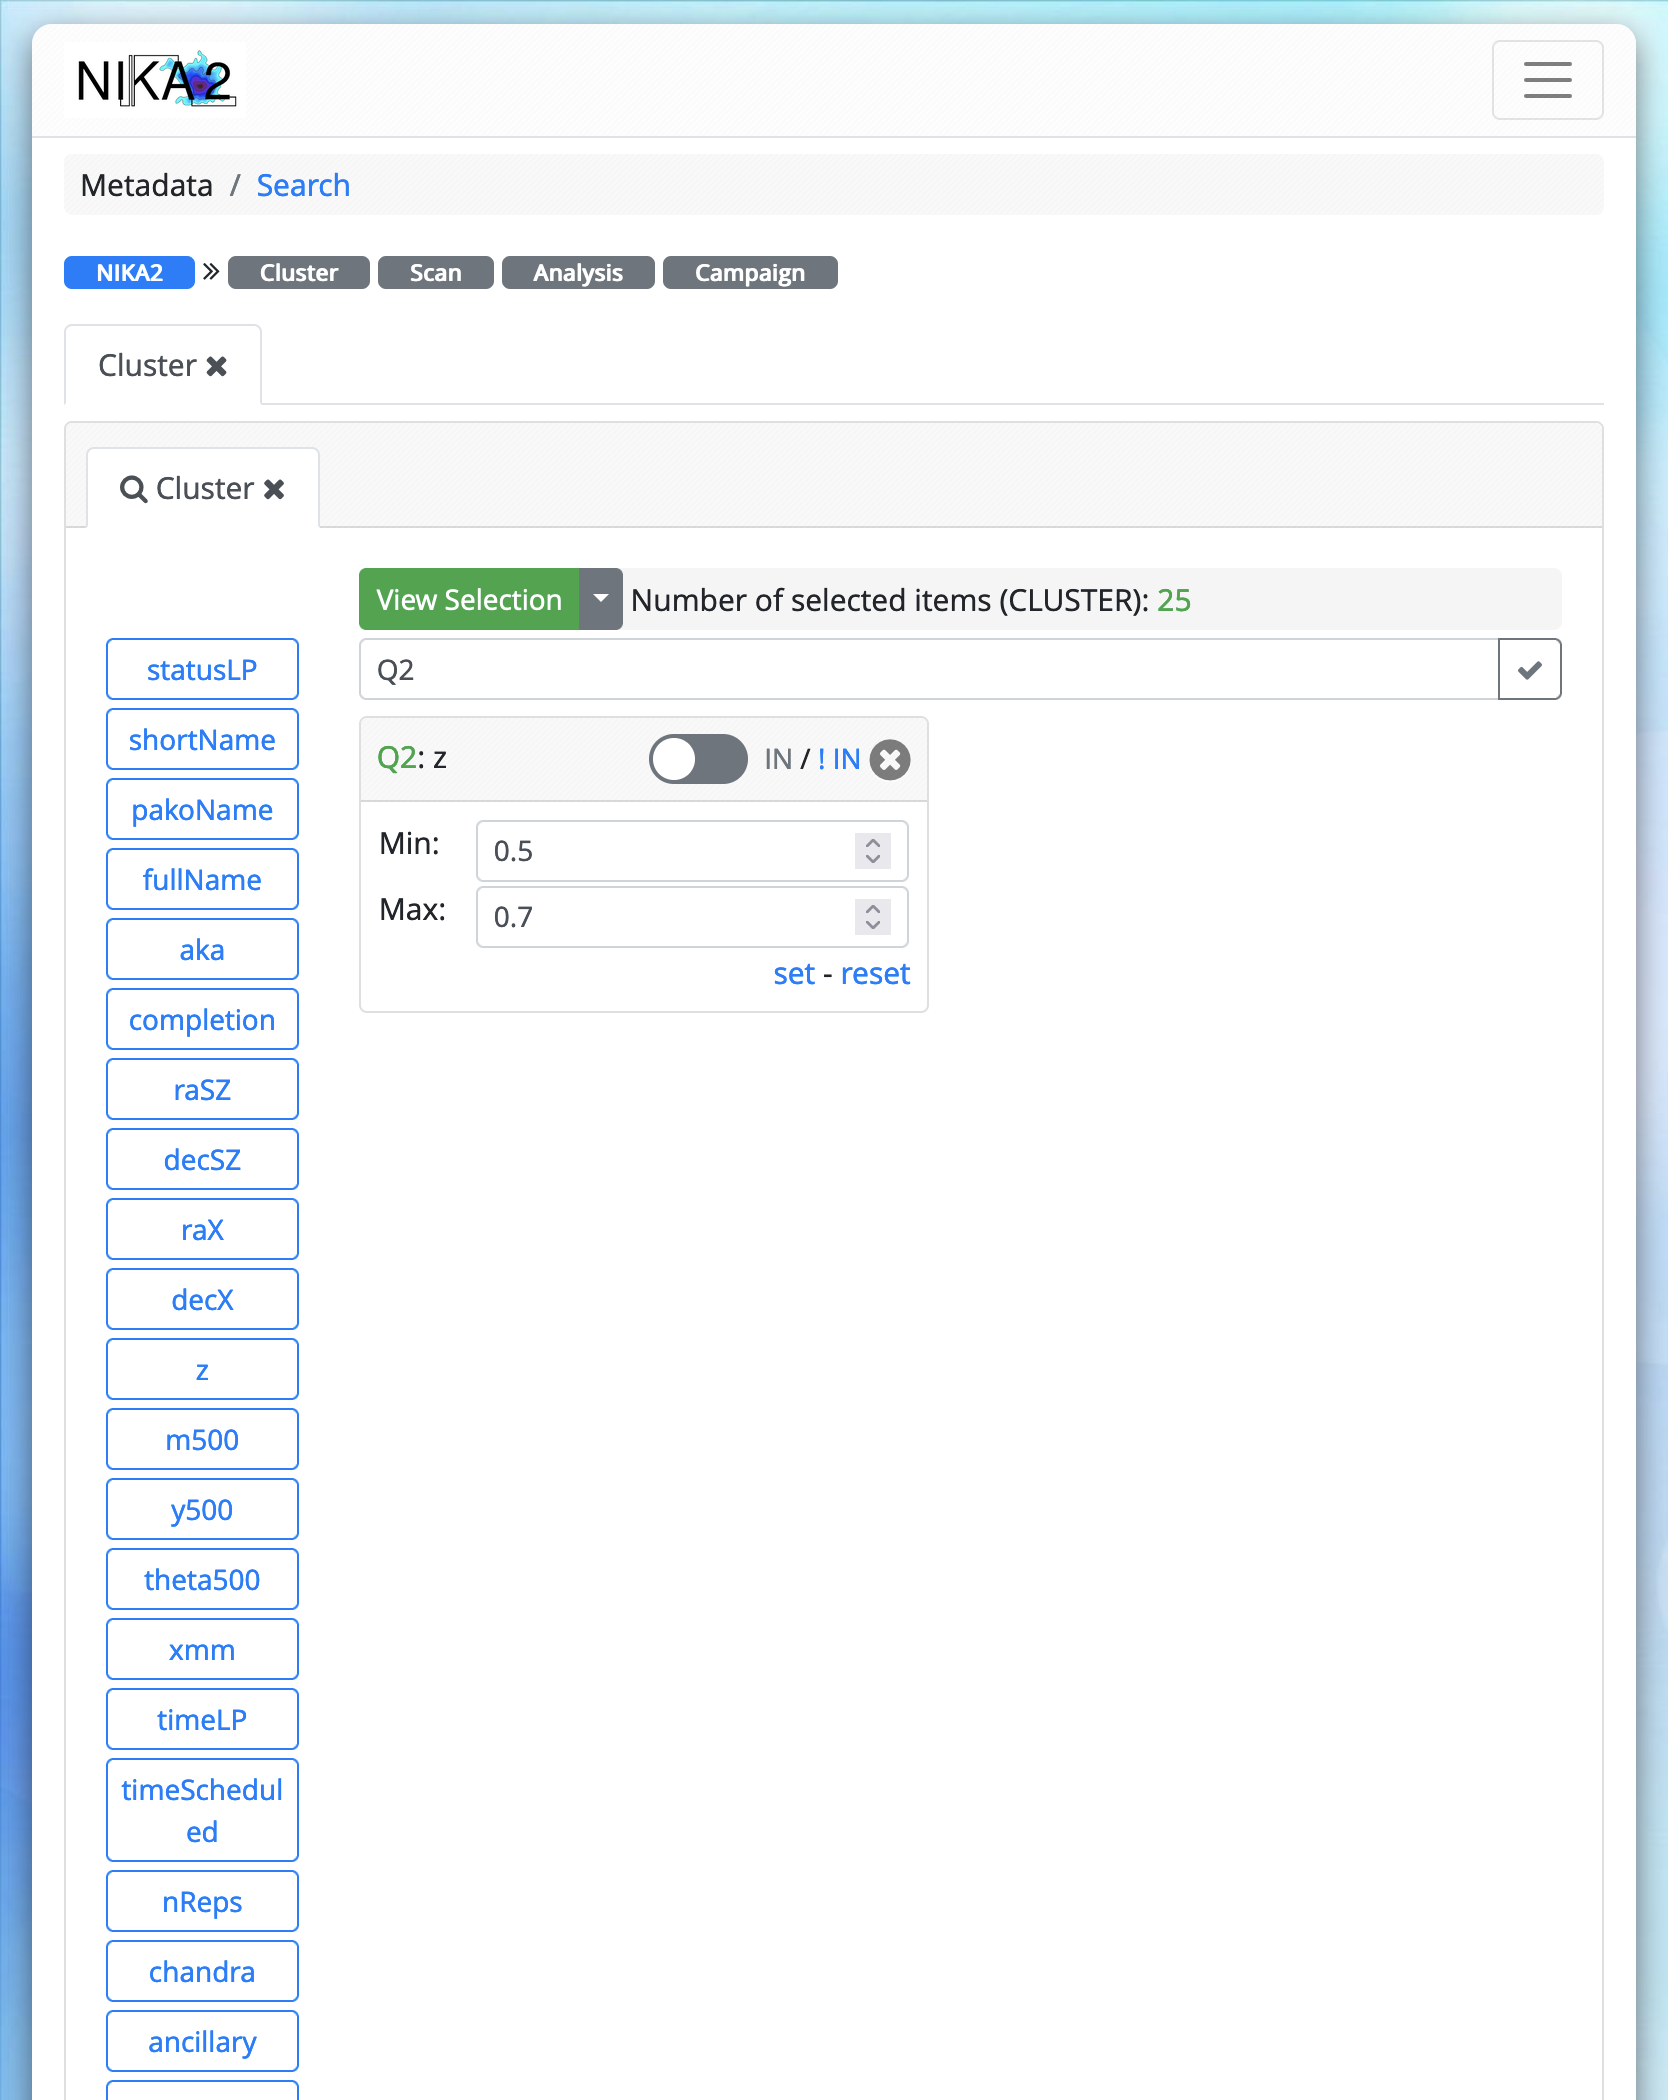
\includegraphics[width=.49\linewidth, trim={0 12cm 0 0}, clip]{Figures/Chap_nk/ami_query_1.png} \hfill
    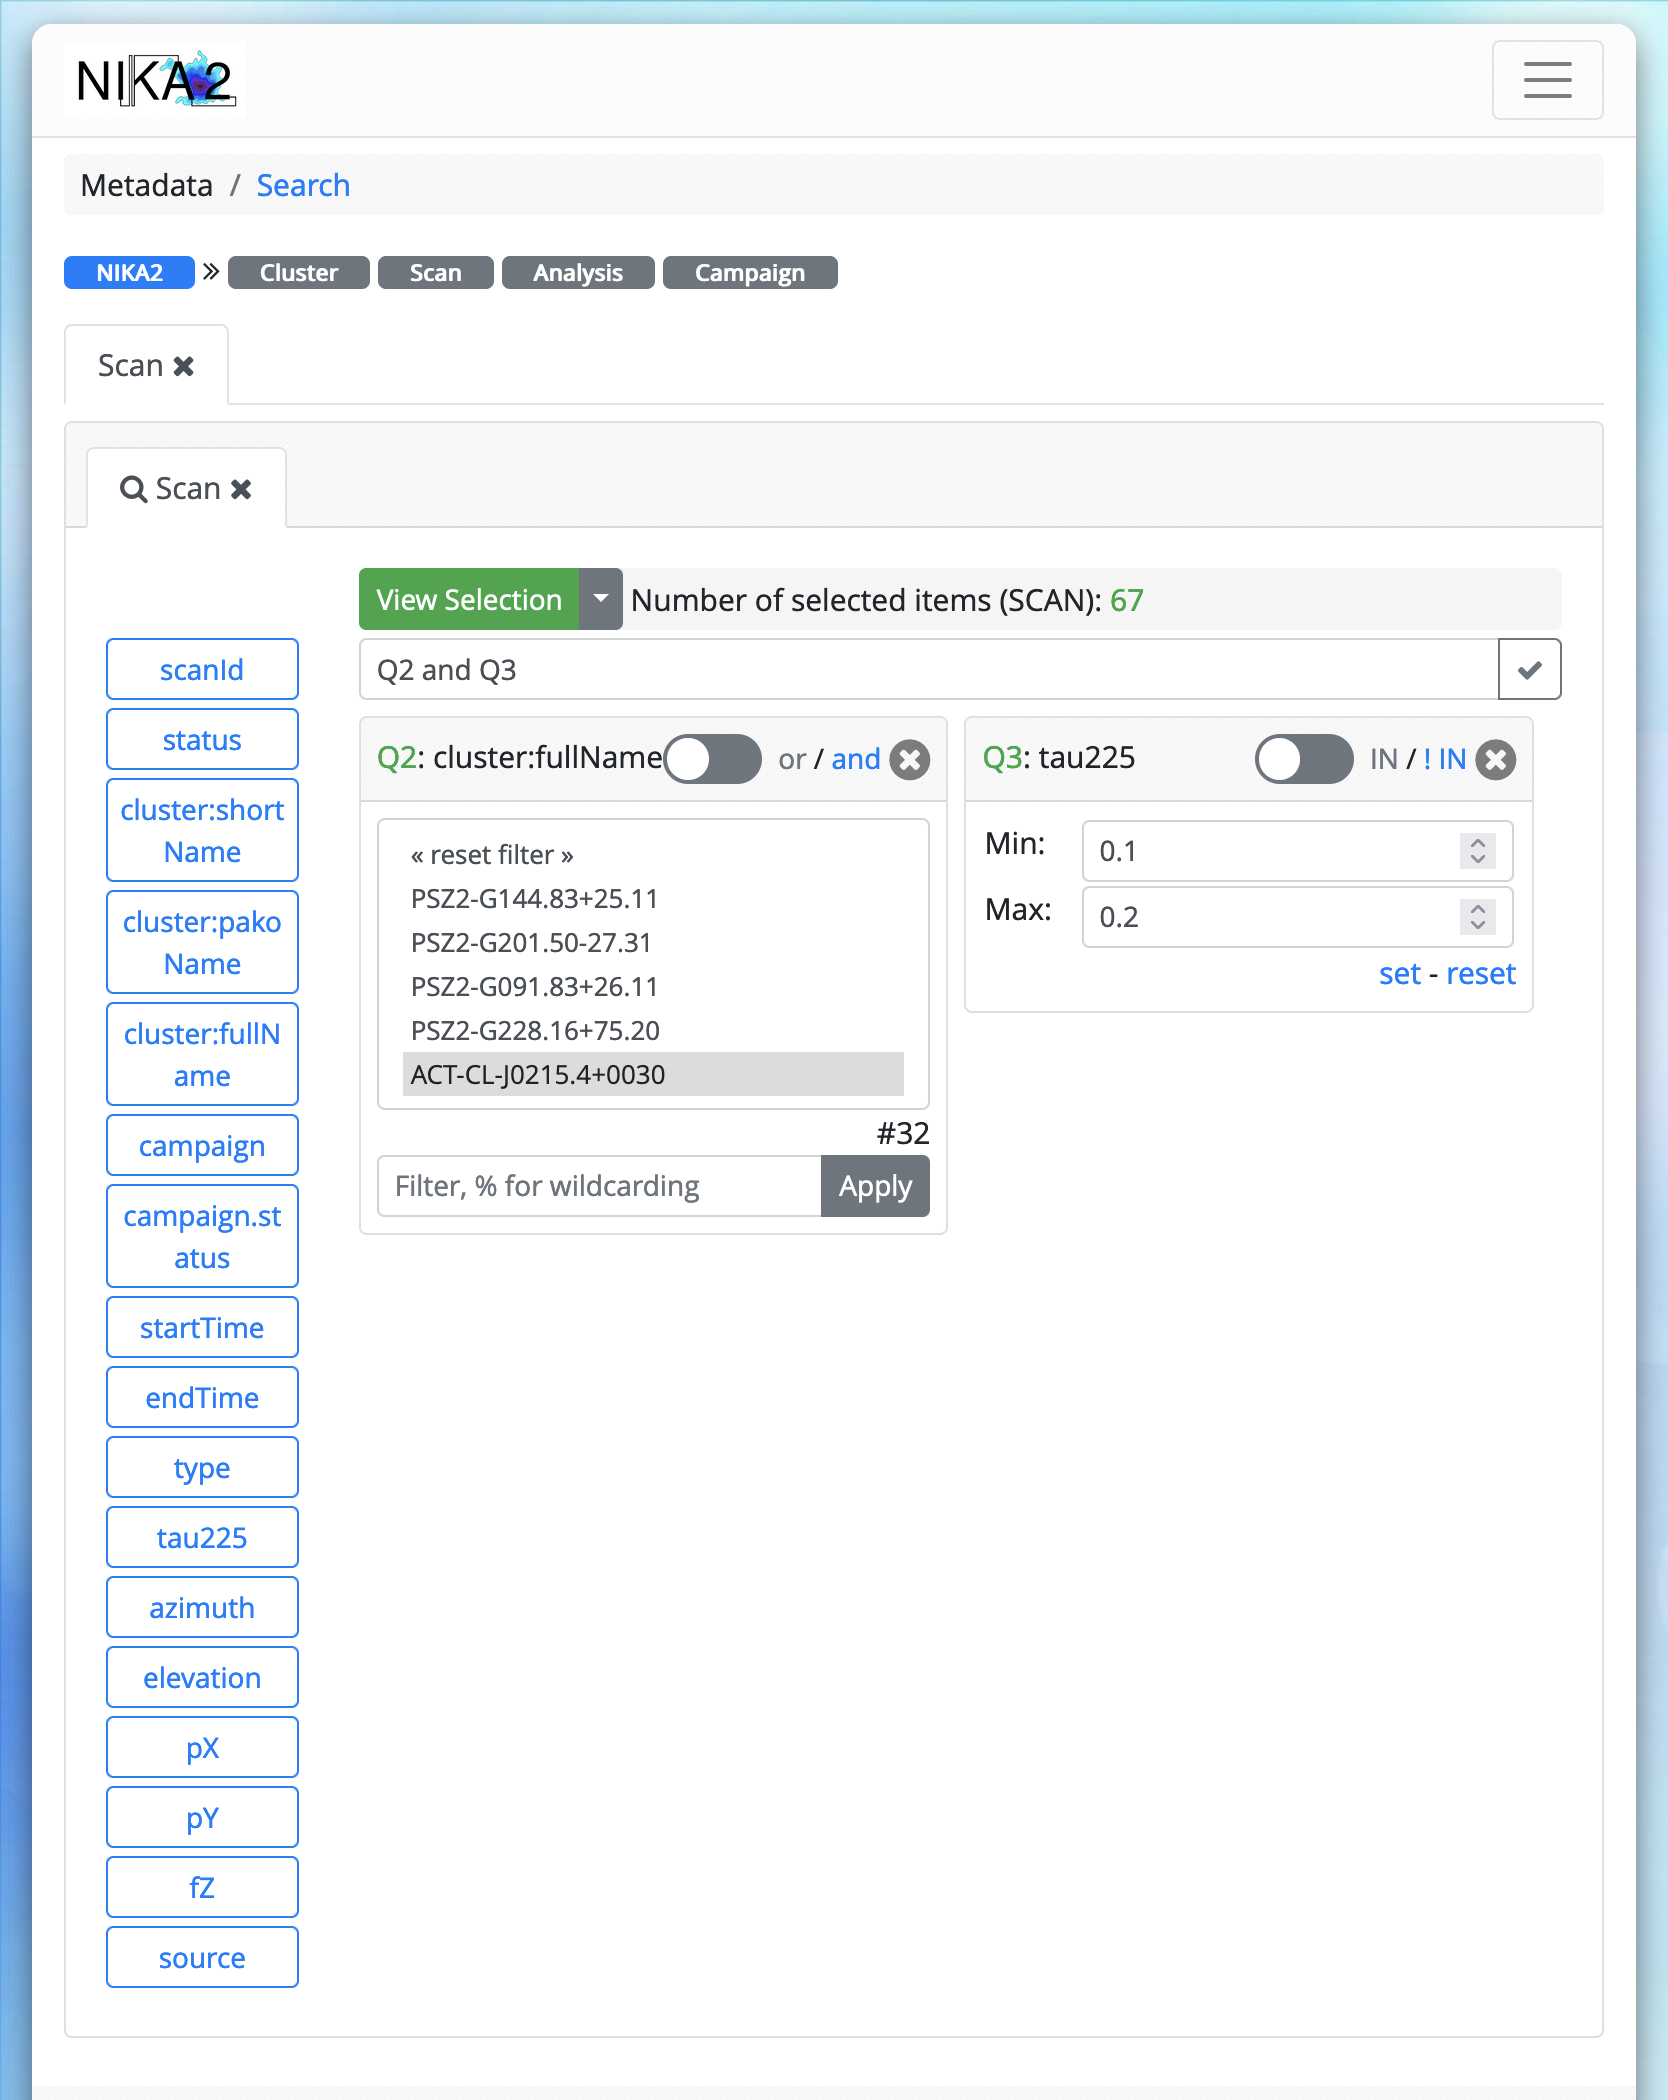
\includegraphics[width=.49\linewidth, trim={0 12cm 0 0}, clip]{Figures/Chap_nk/ami_query_2.png}
    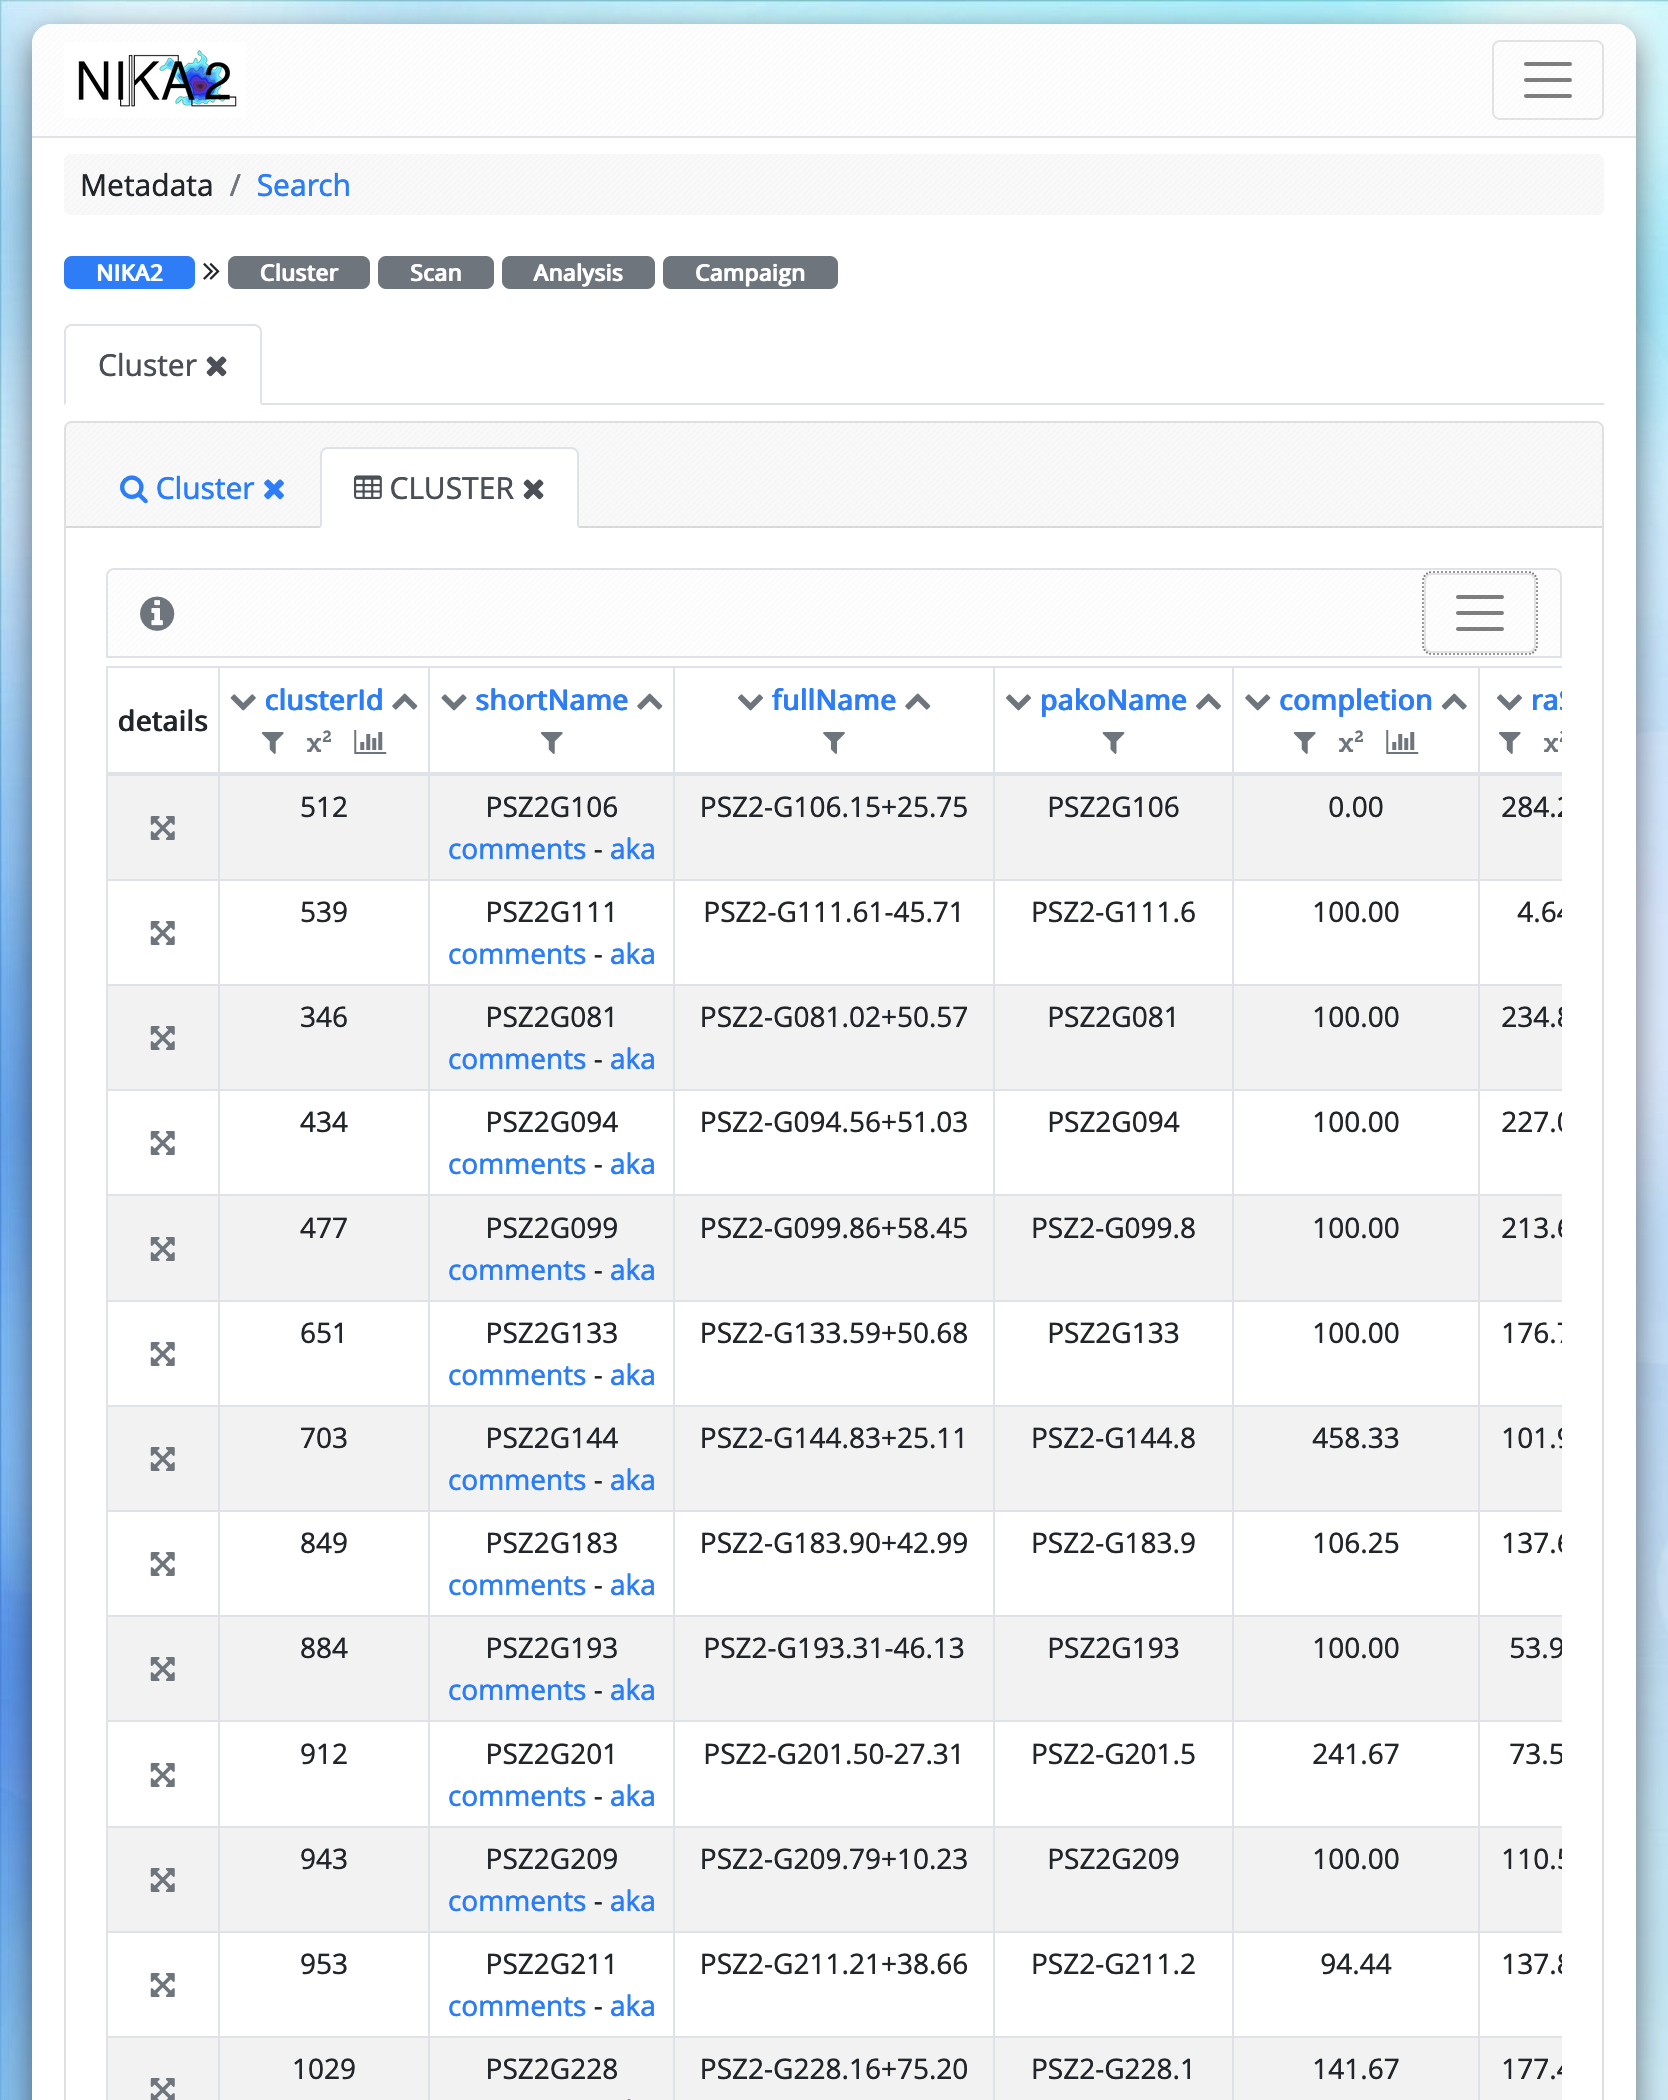
\includegraphics[width=.49\linewidth, trim={0 12cm 0 0}, clip]{Figures/Chap_nk/ami_results_1.png} \hfill
    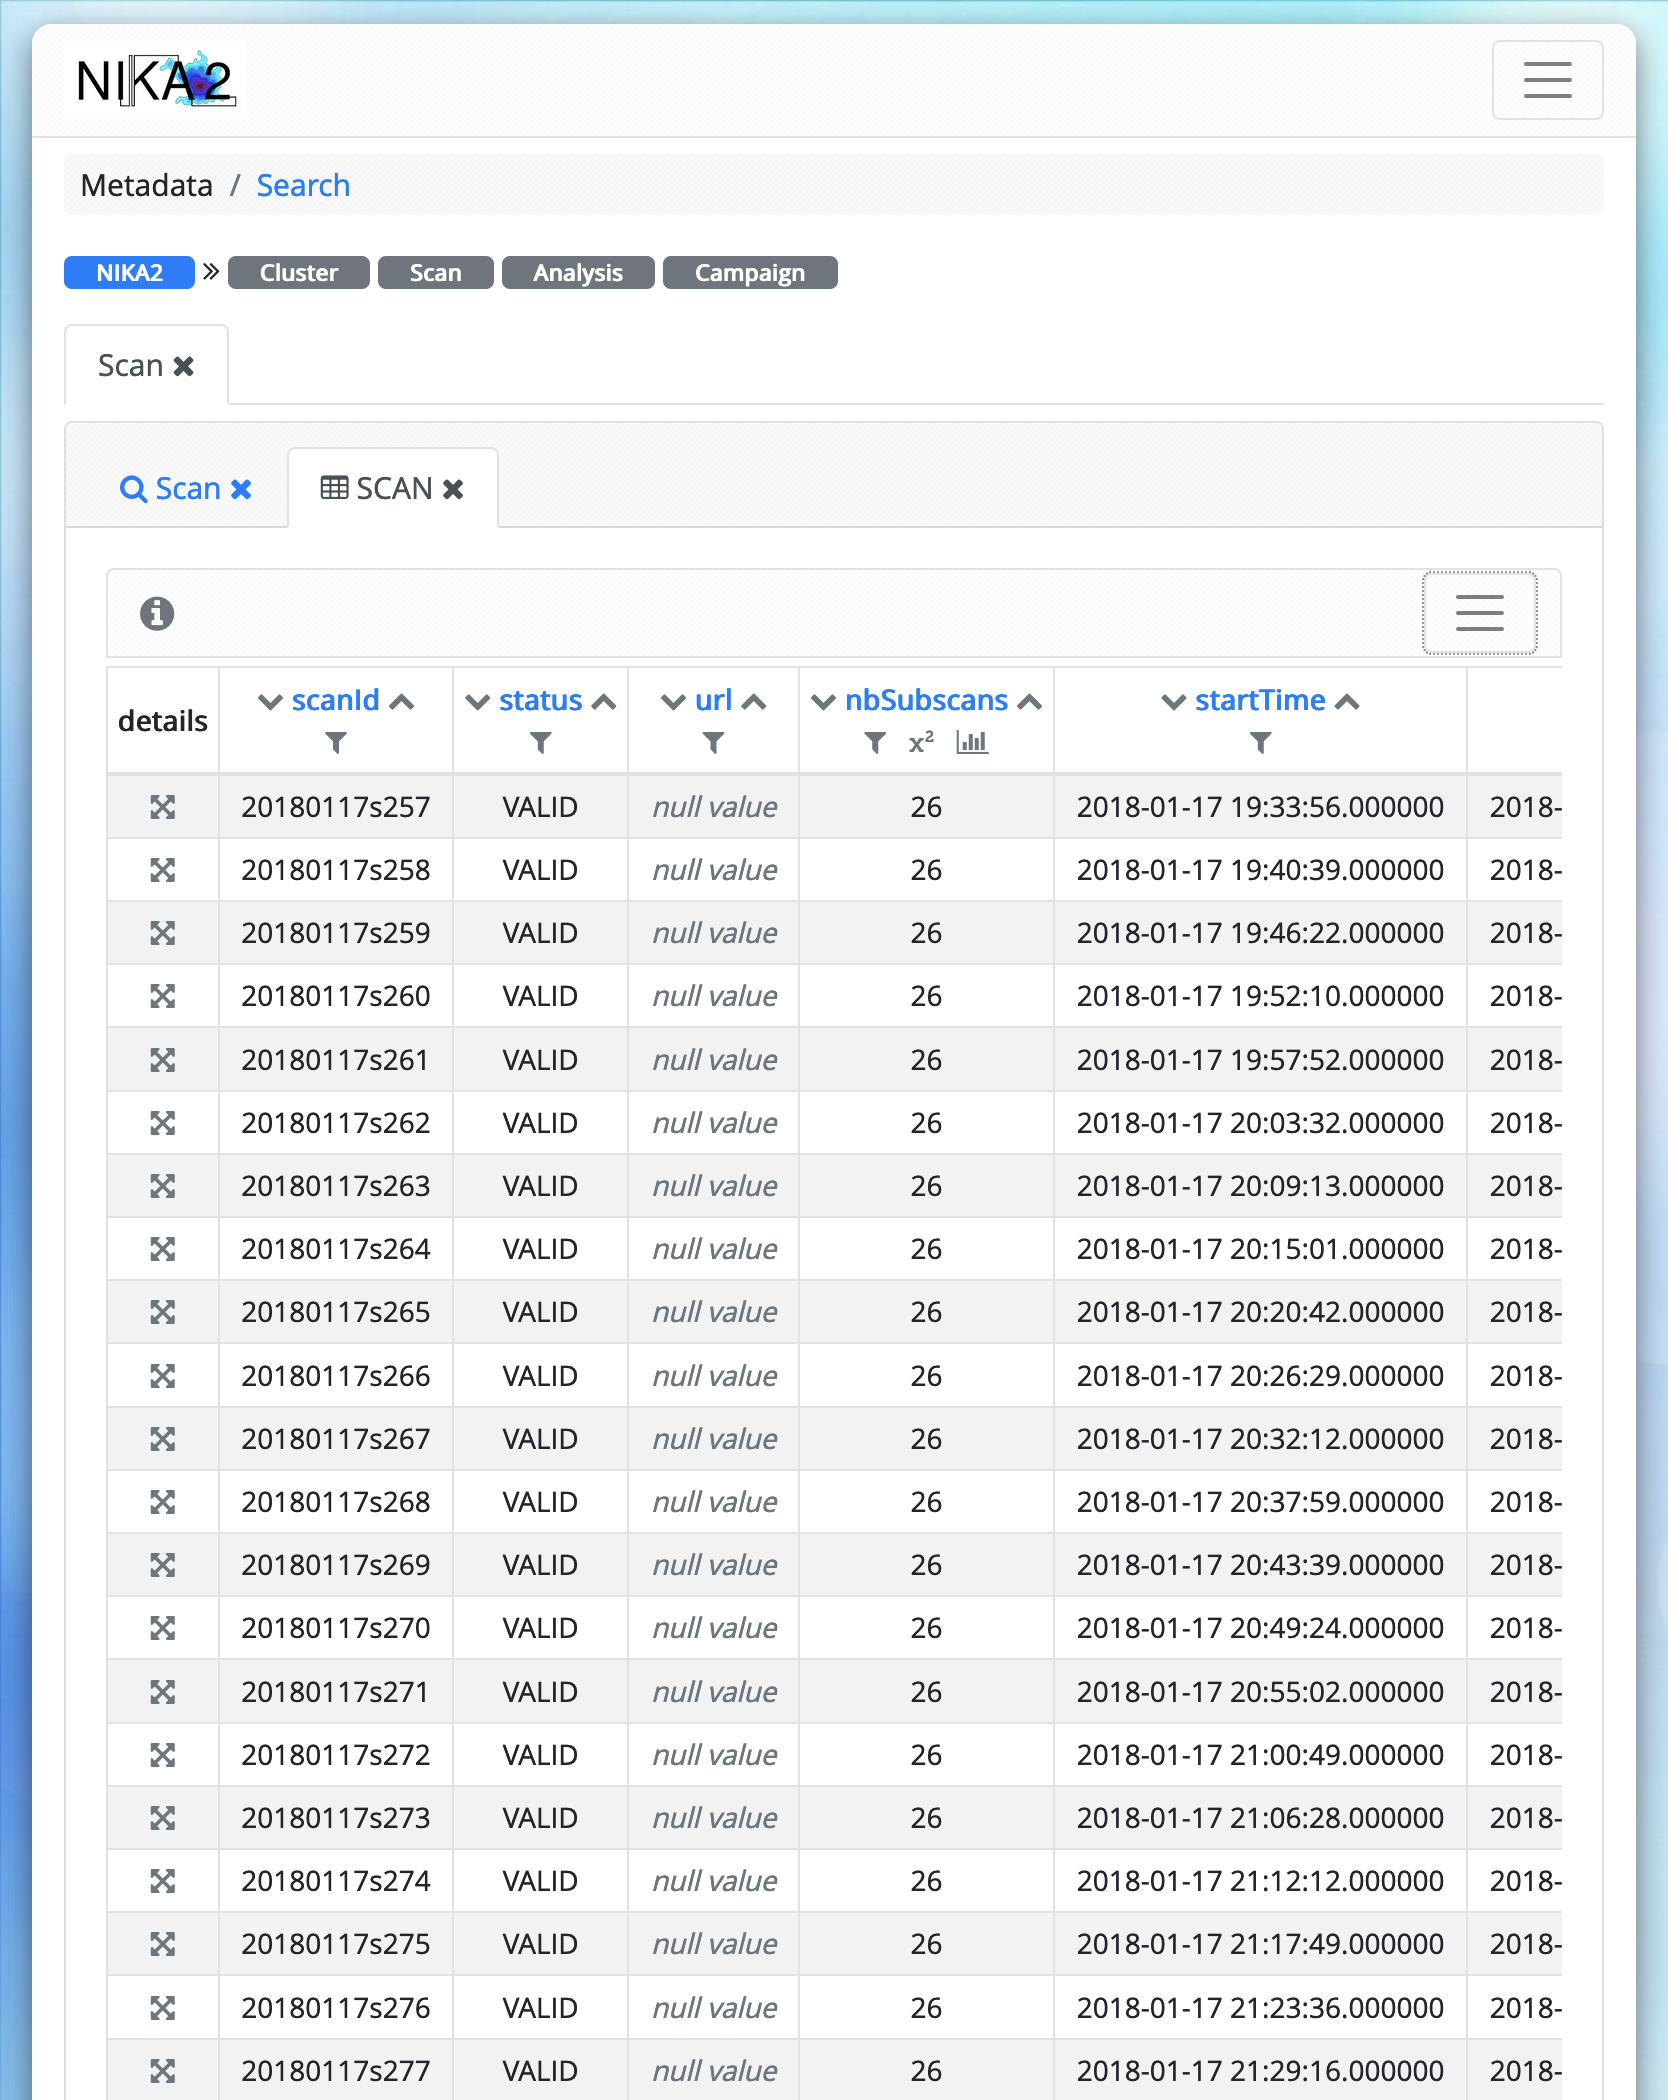
\includegraphics[width=.49\linewidth, trim={0 12cm 0 0}, clip]{Figures/Chap_nk/ami_results_2.png}
    \caption{
        Deux exemples de requêtes dans l'interface graphique de AMI (\textit{haut}) et leurs résultats (\textit{bas}).
        \textbf{Gauche:} recherche des amas du grand programme SZ dont le redshift est compris entre 0.5 et 0.7.
        \textbf{Droite:} recherche des \textit{scans} de l'amas \act\ ayant été effectués pour une opacité atmosphérique $\tau_{225}$ entre 0.1 et 0.2.
    }
    \label{fig:ami_request}
\end{figure*}

La base de données peut également être interrogée en Python.
Cette fonctionnalité est particulièrement intéressante pour interfacer les logiciels de traitement de données du grand programme SZ avec la base de données AMI-LPSZ.
Par exemple, le traitement des données brutes de NIKA2 décrit au chapitre \ref{chap:decorr} nécessite de connaître la liste des \textit{scans} associés à l'amas considéré.
Cette liste est facilement accessible grâce à l'interface Python, ce qui simplifie grandement le processus.
Il est également possible d'utiliser cette interface pour créer automatiquement les fichiers nécessaires pour les observations au télescope.

% ------------------------------------------------------------------------------------- %
\subsection{Développements futurs}

La base de données AMI-LPSZ offre un grand nombre de fonctionnalités qui ont déjà énormément facilité la gestion du grand programme SZ.
Certains aspects restent cependant à développer.
L'un des objectifs serait de stocker dans AMI les résultats des différentes étapes de l'analyse des données de chaque amas, de l'analyse des données brutes décrite au chapitre \ref{chap:decorr} aux propriétés thermodynamiques traitées au chapitre \ref{chap:panco}.
Pour l'instant, les résultats d'analyse ne sont pas stockés sur la base de données, car la structure des métadonnées à y sauvegarder n'a pas été définie.
De plus, la gestion des données externes est pour l'instant sommaire.
L'information sur ces données est consignée dans un champ correspondant à un dictionnaire clé-valeur pour chaque amas.
Dans ce champ, chaque clé indique le nom d'un instrument (\textit{XMM-Newton} ou \textit{Chandra} pour les observations X, SPIRE, PACS ou FIRST pour les sources ponctuelles, etc), et la valeur associée est un booléen, indiquant l'existence ou non de données correspondant à chaque instrument.
Un objectif de la base de donnée serait de compléter ces champs avec plus d'information, par exemple l'adresse à laquelle les données peuvent être récupérées.
Cette base de données représente donc un outil déjà extrêmement utile pour le grand programme SZ de NIKA2, mais qui pourra le devenir encore plus avec une définition de la structure des données pertinentes à stocker pour les données externes et les résultats d'analyse.


% ------------------------------------------- %
\chapter{Construction de cartes de l'effet SZ avec NIKA2}
\label{chap:decorr}
\minitoc
Dans le chapitre précédent, nous avons décrit l'instrument NIKA2, installé au télescope de 30 mètres de l'IRAM, et ses performances.
Nous avons vu en quoi ses performances étaient parfaitement adaptées aux observations de l'effet SZ en direction d'amas de galaxies, et expliqué comment sont réalisées les observations avec NIKA2.

Dans ce chapitre, nous présentons la procédure employée pour produire des cartes de l'effet SZ avec NIKA2.
Comme nous l'avons vu, les données brutes de l'instrument sont des données ordonnées en temps, ou TOI, donnant pour chaque détecteur de NIKA2 l'évolution de la puissance lumineuse reçue au cours d'un mouvement de balayage du ciel.
Nous détaillons les différentes composantes de ces TOI, et la méthode utilisée pour en isoler le signal d'intérêt, et le projeter en une carte du ciel.
Nous présenterons enfin l'évaluation des performances de cette procédure au travers de deux critères: l'évaluation du bruit résiduel dans les données, et du filtrage subi par le signal d'intérêt.
Ces critères sont également des outils utilisés pour tenir compte des systématiques que représentent le filtrage du signal et du bruit résiduel caractéristiques des cartes d'amas construites à partir des observations NIKA2, comme nous le verrons au chapitre \ref{chap:panco}.
Nous présenterons également le logiciel \texttt{PSTools}, développé au cours de cette thèse, dont l'objectif est d'estimer l'amplitude de la contamination de l'effet SZ par des sources submillimétriques.

% ===================================================================================== %
\section{Composantes des données en temps}

Au cours des observations avec NIKA2, le ciel est balayé suivant un motif donné pour enregistrer la variation de fréquence de résonance des KID de l'instrument, qui est ensuite convertie en variation de puissance lumineuse par la procédure d'étalonnage.
Malheureusement, plusieurs composantes viennent s'ajouter à ces données en temps, en plus du signal astrophysique d'intérêt.
La TOI d'un KID $k$ à une fréquence $\nu$ est donc la somme de ces différentes composantes, et peut s'écrire:
\begin{equation}
    \label{eq:toi}
    {\rm TOI}_k(t, \nu) = S_k(t, \nu) + \alpha_k(t) A_k(t, \nu) + \epsilon_k(t) E_k(t) + G_k(t) + C_k(t) + N_k(t),
\end{equation}
L'objectif de la réduction des données est d'isoler la première composante $S_k(t, \nu)$, représentant le signal astrophysique d'intérêt, des autres termes, qui sont des contaminants à ce dernier.
Nous détaillons par la suite la nature de chacun des termes de l'équation (\ref{eq:toi}).

\subsubsection{Signal astrophysique d'intérêt: $S_k(t, \nu)$} % ----------------------- %
L'objectif des observations avec NIKA2 est la production d'une cartographie aussi fidèle que possible du ciel dans les bandes passantes de l'instrument.
Dans le cas des observations du grand programme SZ, les portions du ciel observées contiennent le signal SZ en provenance des amas de galaxies, mais aussi du signal provenant d'autres sources, par exemple des objets astrophysiques d'avant plan (ou d'arrière plan), des galaxies membres de l'amas, le fond diffus cosmologique, ou encore un fond créé par les sources non-résolues (nommé CIB pour \textit{Cosmic Infrared Background}).
L'ensemble de ces constituants forme une carte de la brillance de surface du ciel dans les bandes passantes de NIKA2, notée $M(x, y, \nu)$, où $(x, y)$ représentent les coordonnées célestes.
Lors du balayage de la région par le télescope, un détecteur $k$ à une fréquence $\nu$ enregistre une variation de brillance de surface pouvant s'écrire:
\begin{equation}
    \label{eq:toi_to_map}
    S_k(t, \nu) = P_k(t, x, y) \times M(x, y, \nu),
\end{equation}
où $P_k(t, x, y)$ est la matrice de pointage, décrivant la position du détecteur sur le ciel à un instant $t$:
\begin{equation}
    \label{eq:pointing_matrix}
    P_k(t, x, y) =
        \begin{cases}
            \; 1 \;\text{si le KID $k$ passe par la position $(x, y)$ au temps $t$}, \\
            \; 0 \;\text{sinon.}
        \end{cases}
\end{equation}
Nous verrons en \mypageref{sec:projec_toi} que c'est cette matrice qui est utilisée pour la projection des TOI en une carte après soustraction des autres composantes.

\subsubsection{Bruit atmosphérique: $A_k(t, \nu)$} % ---------------------------------- %
Comme nous l'avons mentionné en section \mypageref{sec:30m_geo}, l'atmosphère est l'un des contaminants principaux des observations millimétriques.
En effet, l'atmosphère est caractérisée non seulement par une absorption qui atténue le signal reçu (voir figure \ref{fig:30m}), mais également par une émission aux longueurs d'onde millimétriques.
Dans le domaine millimétrique, cette émission est bien modélisée par une émission de corps gris, et suit:
\begin{equation}
    I_{\rm atm.}(\nu) \propto \nu^2 T_{\rm atm.} \big[ 1 - \exp(-\tau_\nu / \sin(el)) \big],
\end{equation}
où $T_{\rm atm.}$ est la température de l'atmosphère, $\tau_\nu$ l'opacité au zénith à la fréquence $\nu$, détaillée dans l'équation (\ref{eq:tau_trans}), et $el$ l'élévation des observations.

Pour une température donnée, l'émission de l'atmosphère dépend donc de son opacité $\tau_\nu$.
Celle-ci, comme nous l'avons détaillé en \mypageref{sec:30m_geo}, est dominée par la présence de dioxygène et d'eau dans l'atmosphère.
Le dioxygène étant réparti de façon homogène dans l'atmosphère, son émission thermique ne varie pas spatialement (à élévation constante).
En revanche, la distribution d'eau n'est pas homogène, du fait notamment de la présence de nuages.
Son émission thermique n'est donc pas homogène sur le ciel.
Cette anisotropie est la source principale de la variation temporelle de signal enregistrée par NIKA2 au cours du balayage du ciel par le télescope, même dans les meilleures conditions météorologiques.

Dans le cadre d'observations avec le télescope de 30 mètres de l'IRAM, l'émission atmosphérique vue par les détecteurs à un instant donné est la même.
En effet, la distance de Fraunhofer pour une ouverture $D=30 \;\unit{m}$ vaut $2D^2/\lambda \sim 1000 \;\unit{km}$ aux fréquences d'observation de NIKA2, soit bien au-delà de l'atmosphère.
Celle-ci peut alors être intégrée en champ proche\footnotemark, et on peut l'approximer au premier ordre comme homogène sur le ciel à un temps donné.
\footnotetext{Voir \url{https://www.cv.nrao.edu/~sransom/web/Ch3.html}, section 3.2, ainsi que le chapitre 9 de \cite{adam_observation_2015} pour plus de détails.}
Cette propriété permet d'approximer que l'émission atmosphérique se manifeste de la même façon pour tous les détecteurs dans les TOI obtenues au cours d'un \textit{scan}: on a alors $A_k(t, \nu) = A(t, \nu) \, \forall k$.
Le coefficient $\alpha_k(t)$ de l'équation (\ref{eq:toi}) quantifie alors la réponse de chaque détecteur au bruit atmosphérique.

\subsubsection{Bruit électronique: $E_k(t, \nu)$} % ----------------------------------- %
Nous avons vu dans le chapitre \ref{chap:nika2} que les KID de NIKA2 étaient multiplexés, c'est-à-dire qu'un grand nombre de détecteurs sont lus simultanément par une même ligne de lecture.
L'électronique utilisée pour la lecture de ces signaux induit une composante de bruit non-négligeable.
Celle-ci est, par construction, corrélée pour les détecteurs lus par une même boîte électronique.
Cette propriété de corrélation est utilisée pour isoler la composante de bruit électronique et la soustraire aux données en temps des détecteurs.
Si le bruit atmosphérique est, comme nous l'avons vu dans la section précédente, corrélé entre tous les détecteurs, le bruit électronique ne l'est que pour les détecteurs lus par une même boîte électronique.
Une composante en sous-bande électronique est également présente, corrélée pour les détecteurs couplés à une même ligne de lecture.
Nous verrons en \mypageref{sec:common_mode} qu'il est ainsi possible de traiter les TOI des détecteurs par groupe de KID afin d'isoler au mieux le signal astrophysique d'intérêt du bruit.
Le coefficient $\epsilon_k(t)$ de l'équation (\ref{eq:toi}) représente la réponse de chaque KID $k$ à ce bruit électronique.

\subsubsection{\textit{Glitches} et bruit du cryostat: $G_k(t)$ et $C_k(t)$} % -------- %
Les observations avec NIKA2 sont soumises à d'autres types de contaminants.
Les \textit{glitches} $G_k(t)$ sont des évènements ponctuels dus à l'impact des rayonnements cosmiques sur les détecteurs.
Ceux-ci sont facilement identifiés dans les données en temps, dans lesquelles ils se manifestent comme des pics de Dirac isolés correspondant à des grandes valeurs de flux.

Les KID sont également soumis à un bruit supplémentaire provenant des vibrations du système cryogénique, $C_k(t)$.
Celles-ci ont une signature spectrale très spécifique, se manifestant par une oscillation sinusoïdale dans les données en temps.
Leur contribution au TOI est mesurée dans les transformées de Fourier de ces dernières, dans lesquelles elles apparaissent comme des pics de Dirac isolés.
Elles peuvent donc être soustraites des données.

Ces deux types d'évènement, de nature très différente, ont des contributions aux données en temps des détecteurs également différentes.
Cependant, ces contributions peuvent être identifiées par recherche de pics dans les TOI ou dans leur transformée de Fourier.
Elles peuvent ensuite en être soustraites avant le début de la procédure d'estimation du bruit corrélé.

\subsubsection{Bruit intrinsèque du détecteur: $N_k(t)$} % ---------------------------- %
La dernière composante de l'équation (\ref{eq:toi}) est le bruit intrinsèque des détecteurs $N_k(t)$.
Ce bruit est dominé par les brisures spontanées de paires de Cooper et le bruit de photons.
Il est par nature aléatoire et propre à chaque détecteur, et n'est donc pas corrélé entre les différents KID de NIKA2.
Par conséquent, sa contribution aux données en temps ne peut pas être évaluée, ni donc être soustraite: il s'agit donc de la composante limitant la sensibilité de l'instrument.
%Puisqu'il est propre à chaque détecteur et n'est pas corrélé, il est bien décrit par un bruit blanc.
Ce bruit n'étant pas corrélé entre les différents détecteurs, sa contribution aux cartes du ciel construites à partir des observations NIKA2 est bien décrite par un bruit blanc non-corrélé spatialement.
Par conséquent, une procédure de soustraction des contaminants parfaite peut aboutir à une carte du ciel dans laquelle le bruit est entièrement décorrélé, justifiant les hypothèses de bruit blanc dans les cartes qui seront discutées par la suite.

% ===================================================================================== %
\section{Soustraction du bruit corrélé} \label{sec:decor}

Comme nous l'avons vu dans la section précédente, les données en temps enregistrées par les détecteurs sont la somme du signal astrophysique et de différents types de bruits.
Nous avons vu comment le bruit décorrélé lié aux rayonnements cosmiques et au fonctionnement du cryostat pouvait être retiré des données, grâce à la connaissance des propriétés de ces contributions.
Néanmoins, les contributions les plus importantes de bruit, c'est-à-dire l'émission atmosphérique et le bruit électronique, restent présentes dans les données.
Celles-ci engendrent des variations de brillance de surface de plusieurs Jy au cours d'un \textit{scan}.
À titre de comparaison, la brillance de surface au pic d'un amas de galaxies du grand programme SZ de NIKA2 est de l'ordre du mJy, soit plusieurs ordres de grandeurs plus faible que le bruit.
Il est donc crucial de supprimer ces contributions dans les données afin de cartographier le signal d'intérêt.
Cette procédure se nomme décorrélation, puisque son objectif est de soustraire les composantes de bruit corrélées entre les KID pour ne laisser que le bruit blanc intrinsèque à chaque détecteur.

% ------------------------------------------------------------------------------------- %
\subsection{Estimation de mode commun}\label{sec:common_mode}

Le niveau de bruit présent dans les données peut être estimé grâce à la corrélation entre les différents détecteurs.
Celle-ci permet d'assimiler le bruit corrélé à un mode commun aux TOI des différents KID de NIKA2.
Ce mode commun peut être calculé de plusieurs façons, dont la description progressive permet de comprendre le fonctionnement de l'algorithme de décorrélation et ses performances.

\subsubsection{Mode commun par matrice de KID} % -------------------------------------- %
Comme nous l'avons vu, le signal atmosphérique dans les TOI, qui représente la source majeure de bruit, est le même pour tous les KID d'une matrice de NIKA2.
C'est précisément cette similarité qui peut être exploitée pour retirer la contamination atmosphérique des données.
En effet, le signal d'intérêt, par construction, apparaît comme une composante différente d'un détecteur à un autre, puisque chaque KID voit à un instant donné un point différent du ciel.
Ainsi, la stratégie d'observation pas balayage du ciel fait que chaque KID passe sur la source à un instant différent; le signal astrophysique apparaît donc dans les TOI décalé en temps.
À l'inverse, on peut assimiler l'atmosphère à une source de bruit commune à chacun des détecteurs, et la calculer comme la médiane des TOI de chaque KID considéré\footnotemark.
\footnotetext{On ne considère que les détecteurs valides; voir section \mypageref{sec:focal_plane_reconstruction}.}
L'utilisation de la médiane permet ici de limiter le biais induit par le signal dans l'estimation de la contamination atmosphérique, qui sera discuté plus en détail en section \ref{sec:mask_decor}.

On modélise donc le bruit corrélé dans les observations, dominé par l'atmosphère, comme un mode commun dans les TOI de tous les détecteurs d'une matrice.
Afin de calculer ce mode commun, les TOI de chacun des $N$ détecteurs considérés sont tout d'abord inter-étalonnées sur l'émission atmosphérique, estimée comme la médiane des TOI, en calculant pour chaque KID $k$ un gain $g_k$ d'après:
\begin{equation}
    \label{eq:toi_median}
    {\rm TOI}_k(t, \nu) = g_k \times {\rm Med} \big[{\rm TOI}_{k'}(t, \nu)\big]_{k'}.
\end{equation}
On peut alors calculer le mode commun aux détecteurs comme la moyenne des TOI de tous les KID, pondérée par les gains de ceux-ci:
\begin{equation}
    \label{eq:toi_CM}
    {\rm CM}(t, \nu) = \frac{1}{N} \sum_{k=1}^N \frac{1}{g_k} {\rm TOI}_k(t, \nu).
\end{equation}
Ce mode commun (CM)  peut être soustrait aux données en temps de chaque KID comme un estimateur du bruit corrélé.
Cependant, comme nous l'avons vu dans l'équation (\ref{eq:toi}), chaque détecteur a une réponse différente aux différentes composantes de bruit corrélé.
Afin de tenir compte de ces différentes réponses, on peut calculer un modèle de bruit comme une fonction affine du mode commun pour chaque KID $k$:
\begin{equation}
    \label{eq:toi_noise_CM}
    B_k(t, \nu) = a_k {\rm CM}(t, \nu) + b_k,
\end{equation}
où $a_k$ et $b_k$ sont calculés par régression linéaire pour chaque TOI. \\
En soustrayant cette estimateur de bruit propre à chaque détecteur à ses données en temps, on obtient des données nettoyées d'un mode commun qui, dans l'hypothèse où le bruit est entièrement donné par l'émission atmosphérique, sont dominées par le signal d'intérêt.

Cette procédure est représentée en figure \ref{fig:toi_decor_1CM}.
Celle-ci montre les données en temps de 20 KID de la matrice à 150 GHz de NIKA2 lors d'une observation d'Uranus.
Le panneau gauche montre les données brutes, où on voit le signal astrophysique comme des pics décalés en temps, et le bruit atmosphérique comme le comportement à grande échelle de tous les détecteurs.
Le mode commun estimé sur les TOI de toute la matrice de KID est représenté en rouge.
Sur le panneau droit, on voit les TOI après soustraction de l'estimateur de bruit calculé à partir du mode commun (équation \ref{eq:toi_noise_CM}).
On voit que le comportement à grande échelle du bruit est supprimé, et que seuls restent le signal astrophysique et un bruit mineur, visiblement décorrélé entre les détecteurs.
\begin{figure*}[t]
    \centering
    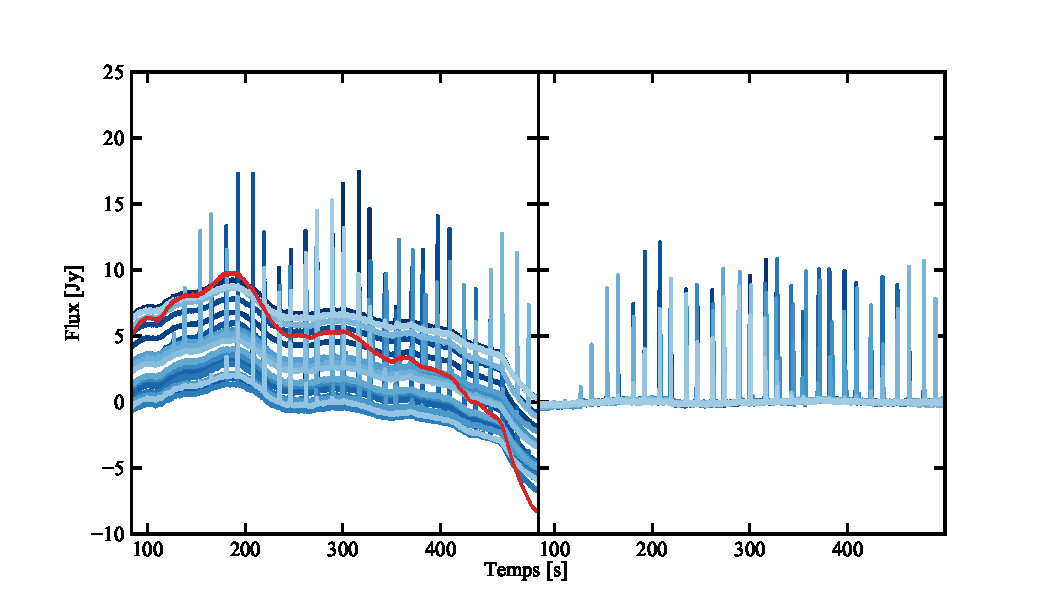
\includegraphics[width=.95\linewidth]{Figures/Chap_decor/toi.pdf}
    \caption{
        \textbf{Gauche:} Données en temps pour 20 détecteurs de la matrice à 150 GHz de NIKA2 lors d'une observation d'Uranus (bleu).
        Le passage de chaque KID sur la planète est visible par les pics d'émission décalés en temps.
        Le mode commun estimé sur les TOI de la matrice entière est représenté en rouge.
    }
    \label{fig:toi_decor_1CM}
\end{figure*}

\subsubsection{Mode commun par boîte électronique} % ---------------------------------- %
Pour la décorrélation illustrée en figure \ref{fig:toi_decor_1CM}, nous avons émis l'hypothèse que le bruit corrélé pouvait être assimilé à un mode commun à tous les KID d'une matrice.
Cette hypothèse repose sur le fait que l'atmosphère est le contaminant dominant dans les données en temps des KID, et que celle-ci est la même pour tous les détecteurs.
Cependant, comme le montre l'équation (\ref{eq:toi}), une autre composante de bruit corrélé est présente dans les données: le bruit dû à l'électronique de lecture.
Celui-ci, par construction, ne présente pas de corrélation entre tous les détecteurs de la matrice, mais seulement entre ceux lus par une même boîte électronique (voir section \ref{sec:kids}, page \pageref{sec:kids}).

Ainsi, à l'issue de la soustraction d'un mode commun atmosphérique, il reste dans les données une composante de bruit corrélé électronique.
Les corrélations entre les KID lors de l'observation d'Uranus présentée en figure \ref{fig:toi_decor_1CM} sont illustrées en figure \ref{fig:toi_corr}.
Sur la gauche sont représentées les corrélations avant soustraction d'un mode commun: tous les détecteurs sont très corrélés entre eux, avec des coefficients de corrélation supérieurs à 99\%.
Sur la droite, on voit les corrélations résiduelles entre les KID après soustraction d'un mode commun calculé sur les TOI de toute la matrice à 150 GHz de NIKA2.
On voit que, si les corrélations sont fortement diminuées -- atteignant des valeurs absolues inférieures à 20\% --, des structures persistent.
En particulier, on remarque deux types de corrélations résiduelles.
Les carrés qui apparaissent corrélés, délimités par des lignes pointillées noires, correspondent aux KID lus par une même boîte électronique.
Les structures carrées plus petites correspondent quant à elles aux détecteurs couplés à la même ligne de lecture.
Ces corrélations montrent l'imperfection de la décorrélation par soustraction d'un seul mode commun pour tous les KID d'une matrice.

\begin{figure*}[t]
    \centering
    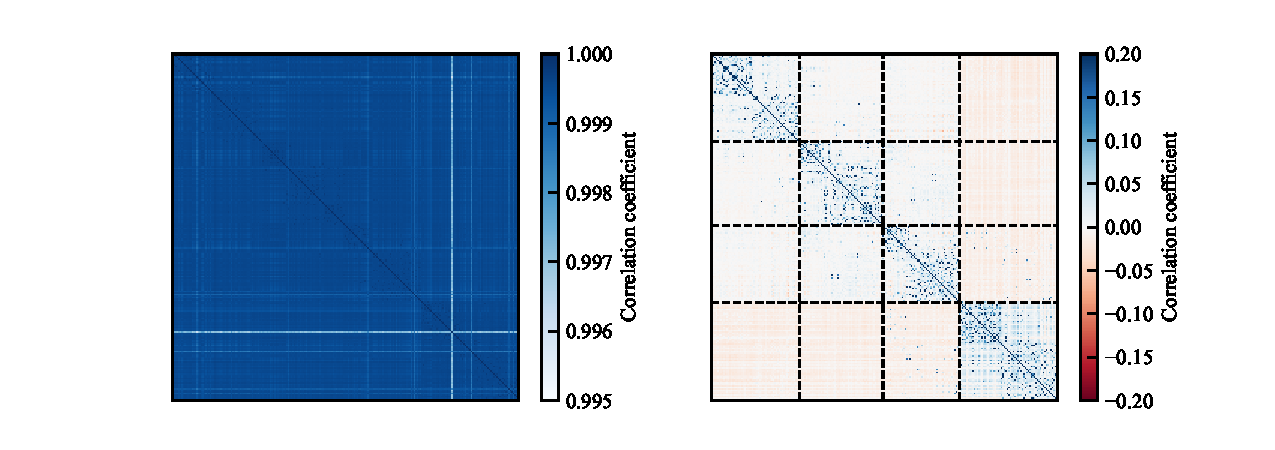
\includegraphics[width=\linewidth, trim={2.3cm .5cm 1.5cm .5cm}, clip]{Figures/Chap_decor/toi_correlation.pdf}
    \caption{
        Matrice de corrélation entre les TOI des détecteurs de la matrice NIKA2 à 150 GHz lors d'une observation d'Uranus.
        \textbf{Gauche:} Corrélations des données brutes, avant soustraction d'un mode commun.
        \textbf{Droite:} Corrélations après soustraction d'un mode commun calculé à partir de tous les détecteurs de la matrice.
        Les lignes noires pointillées délimitent les détecteurs appartenant à chacune des quatre boîtes de l'électronique de lecture de NIKA2.
    }
    \label{fig:toi_corr}
\end{figure*}

Le bruit électronique est en général plus faible que le bruit atmosphérique, bien que les deux composantes puissent avoir une contribution comparable dans le cas d'observations avec d'excellentes conditions météorologiques.
Dans le cas des observations d'Uranus utilisées à titre illustratif en figures \ref{fig:toi_decor_1CM} et \ref{fig:toi_corr}, le bruit électronique est plusieurs ordres de grandeur plus faible que le signal de la planète, d'une dizaine de Jy.
Cependant, pour les observations de l'effet SZ, donc la brillance de surface est au maximum de l'ordre du mJy, le bruit électronique n'est plus négligeable.
Il est donc important, au même titre que pour l'atmosphère, de le retirer des TOI.

Pour ce faire, la procédure d'estimation d'un mode commun détaillée précédemment peut être utilisée, avec une modification notable.
Plutôt que de calculer un mode commun pour tous les détecteurs d'une matrice, la même opération peut être réalisée par groupe de KID, en particulier en les regroupant selon la boîte électronique par laquelle ils sont lus.
Les modes communs résultants contiennent donc à la fois le bruit atmosphérique et le bruit électronique.
D'après l'équation (\ref{eq:toi}), les composantes des TOI restant après soustraction de ce mode commun ne contiennent donc \prior\ plus que le signal d'intérêt et le bruit intrinsèque aux détecteurs.

\subsubsection{Mode commun par groupe de détecteurs corrélés} % ----------------------- %
La décorrélation par ligne de lecture permet donc de tenir compte de deux corrélations différentes entre les KID: celle entre tous les détecteurs d'une matrice, engendrée par le bruit atmosphérique, et celle entre les détecteurs lus par une même électronique de lecture.
D'autres corrélations peuvent être présentes dans les données, mais celles-ci sont difficiles à quantifier: on parle alors de corrélations résiduelles.
On voit notamment dans le panneau droit de la figure \ref{fig:toi_corr} des corrélations entre KID couplés à une même ligne de lecture.
Celles-ci se manifestent par des blocs carrés dans la matrice de corrélation des détecteurs, environ deux fois plus petits que les blocs de KID associés à la même boîte électronique.

Afin d'éliminer au mieux ces corrections résiduelles, on peut procéder à un calcul de mode commun entre détecteurs corrélés.
Pour cela, la matrice de corrélation entre les TOI de tous les détecteurs est calculée.
Les détecteurs sont ensuite groupés par bloc de détecteurs les plus corrélés, indépendamment de toute autre considération (par exemple, de la ligne de lecture à laquelle ils sont couplés).
Un mode commun est calculé pour chacun de ces groupes de KID corrélés, et soustrait de la même façon que pour les méthodes à mode commun par matrice ou par boîte électronique.

Cette méthode est à l'heure actuelle la méthode privilégiée au sein de la collaboration NIKA2, et en particulier pour les observations du grand programme SZ, pour deux raisons principales.
Tout d'abord, comme l'a montré la progression au cours de cette section, elle représente l'aboutissement de la réflexion sur l'exploitation des corrélations entre détecteurs pour retirer le bruit corrélé des données en temps.
De plus, au cours de nombreux tests de différentes méthodes sur des simulations comme sur des données réelles, c'est celle qui a livré les meilleures performances, à la fois en termes de bruit résiduel et de filtrage du signal.
Le filtrage et le bruit résiduel, utilisés à la fois comme métriques pour juger de la qualité du processus de décorrélation et comme outils pour tenir compte des caractéristiques de ce processus lors de l'analyse des cartes, seront discutés en section \mypageref{sec:perf_decor}.
Cette méthode de décorrélation est nommée \textit{common mode one block} dans le pipeline d'analyse des données de la collaboration NIKA2, et décrite dans \cite{perotto_calibration_2020} sous le nom de \textit{most correlated pixels}.

% ------------------------------------------------------------------------------------- %
\subsection{Masquage de source et analyse itérative}\label{sec:mask_decor}

L'estimation du bruit par calcul d'un mode commun permet donc d'obtenir des données en temps dominées par le signal pour chaque détecteur.
Cependant, il faut noter que cette opération est imparfaite: le mode commun des TOI est affecté par la présence de signal dans ces dernières.
Si cet effet est atténué par l'utilisation de la médiane des TOI dans l'estimation des modes communs, il n'est pas complètement annulé.
En particulier, si une proportion significative des détecteurs utilisés dans l'estimation du mode commun passe sur la source au même instant, le mode commun à cet instant contiendra une partie du signal d'intérêt, qui sera soustraite au données et donc perdue dans les cartes.
Le mode commun est donc biaisé par la présence de signal.
Ce biais est d'autant plus important que la source est étendue, puisque la probabilité que deux détecteurs la voient en même temps s'en retrouve augmentée; il est donc particulièrement important dans le cas de l'effet SZ, et \prior\ peu présent pour les sources ponctuelles.
De plus, la méthode d'estimation du mode commun par bloc de détecteurs corrélés augmente par construction l'ampleur de ce biais.
En effet, si la corrélation des TOI pour construire les blocs de données en temps est calculée sans faire la différence entre signal et bruit, des détecteurs voyant simultanément un signal similaire seront corrélés non seulement à cause du bruit, mais également à cause du signal.
Ils auront donc une plus grande corrélation que deux détecteurs voyant la source à des instants différents, et seront groupés pour l'estimation du mode commun.

C'est pourquoi il est important de traiter différemment le signal du bruit au cours de l'estimation du mode commun.
La méthode employée est l'utilisation d'un masque, permettant de ne pas tenir compte des régions contenant du signal dans l'estimation du mode commun.
Ce masque est défini comme la région du ciel contenant du signal astrophysique:
\begin{equation}
    M(x, y) =
        \begin{cases}
            \; 0 \;\text{si du signal est attendu aux coordonnées $(x, y)$}, \\
            \; 1 \;\text{sinon.}
        \end{cases}
\end{equation}
En combinant ce masque avec la matrice de pointage de chaque KID, définie par l'équation (\ref{eq:pointing_matrix}), on peut calculer un masque $M_k(t)$ pour les données en temps de chaque KID,
\begin{equation}
    \label{eq:mask_time}
    M_k(t) = P_k(t, x, y) \times M(x, y) =
        \begin{cases}
            \; 0 \;\text{si du signal est attendu pour le KID $k$ au temps $t$}, \\
            \; 1 \;\text{sinon.}
        \end{cases}
\end{equation}
Le calcul de mode commun décrit précédemment peut donc être réalisé en considérant uniquement les régions des TOI dans lesquelles le masque est non-nul.
Cela permet d'éviter au mode commun d'être biaisé par le signal d'intérêt, puisque les régions contenant du signal ne seront pas considérées dans le calcul du mode commun.

Le calcul du masque requiert donc une connaissance préalable de la région contenant du signal d'intérêt.
Cette opération est délicate, puisque la distinction des contributions du signal et du bruit est l'objectif même de la procédure de décorrélation.
On ne connait donc pas la forme du signal au début de la procédure de décorrélation.
Dans le cadre des observations d'amas de galaxies avec NIKA2, le masque est défini de façon itérative.
Une première estimation du masque est réalisée \prior\ en considérant un disque, centré sur les coordonnées de l'amas, et de rayon suffisamment grand pour inclure tout le signal significatif provenant de l'amas.
La décorrélation par calcul d'un mode commun par blocs de détecteurs corrélés est réalisée dans un premier temps en utilisant ce masque, donnant une première estimation de la distribution du signal astrophysique d'intérêt dans les données en temps de chaque détecteur.
Cette procédure est appliquée pour tous les \textit{scans} réalisés pour l'observation d'un amas.
Les données en temps obtenues, dominées par le signal d'intérêt, sont projetées en cartes du ciel correspondant à chaque \textit{scan}, qui sont ensuite coadditionnées pour obtenir une unique carte de la région de l'amas.
Les procédures de projection et de coaddition seront détaillées en section \mypageref{sec:projec_toi}.
La carte obtenue est utilisée pour déterminer une nouvelle réalisation du masque.
Pour cela, une carte de signal-sur-bruit est calculée comme le rapport entre les cartes de signal astrophysique et de bruit obtenues par la procédure de coaddition.
La région du ciel dans laquelle on détecte un signal astrophysique significatif est utilisée pour mettre à jour le masque $M(x, y)$:
\begin{equation}
    M(x, y) =
        \begin{cases}
            \; 0 \;\text{si le signal-sur-bruit est supérieur à $3\sigma$ aux coordonnées $(x, y)$}, \\
            \; 1 \;\text{sinon.}
        \end{cases}
\end{equation}
La décorrélation est alors répétée avec ce nouveau masque, qui représente une estimation plus fiable de la distribution de signal astrophysique dans la région cartographiée que le masque initial.
La procédure est alors répétée plusieurs fois, en affinant à chaque itération la connaissance du masque grâce à l'itération précédente.
La décorrélation converge alors vers une carte finale, et après quelques ($\sim 5$) itérations, le masque n'évolue plus significativement.

\begin{figure*}[t]
    \centering
    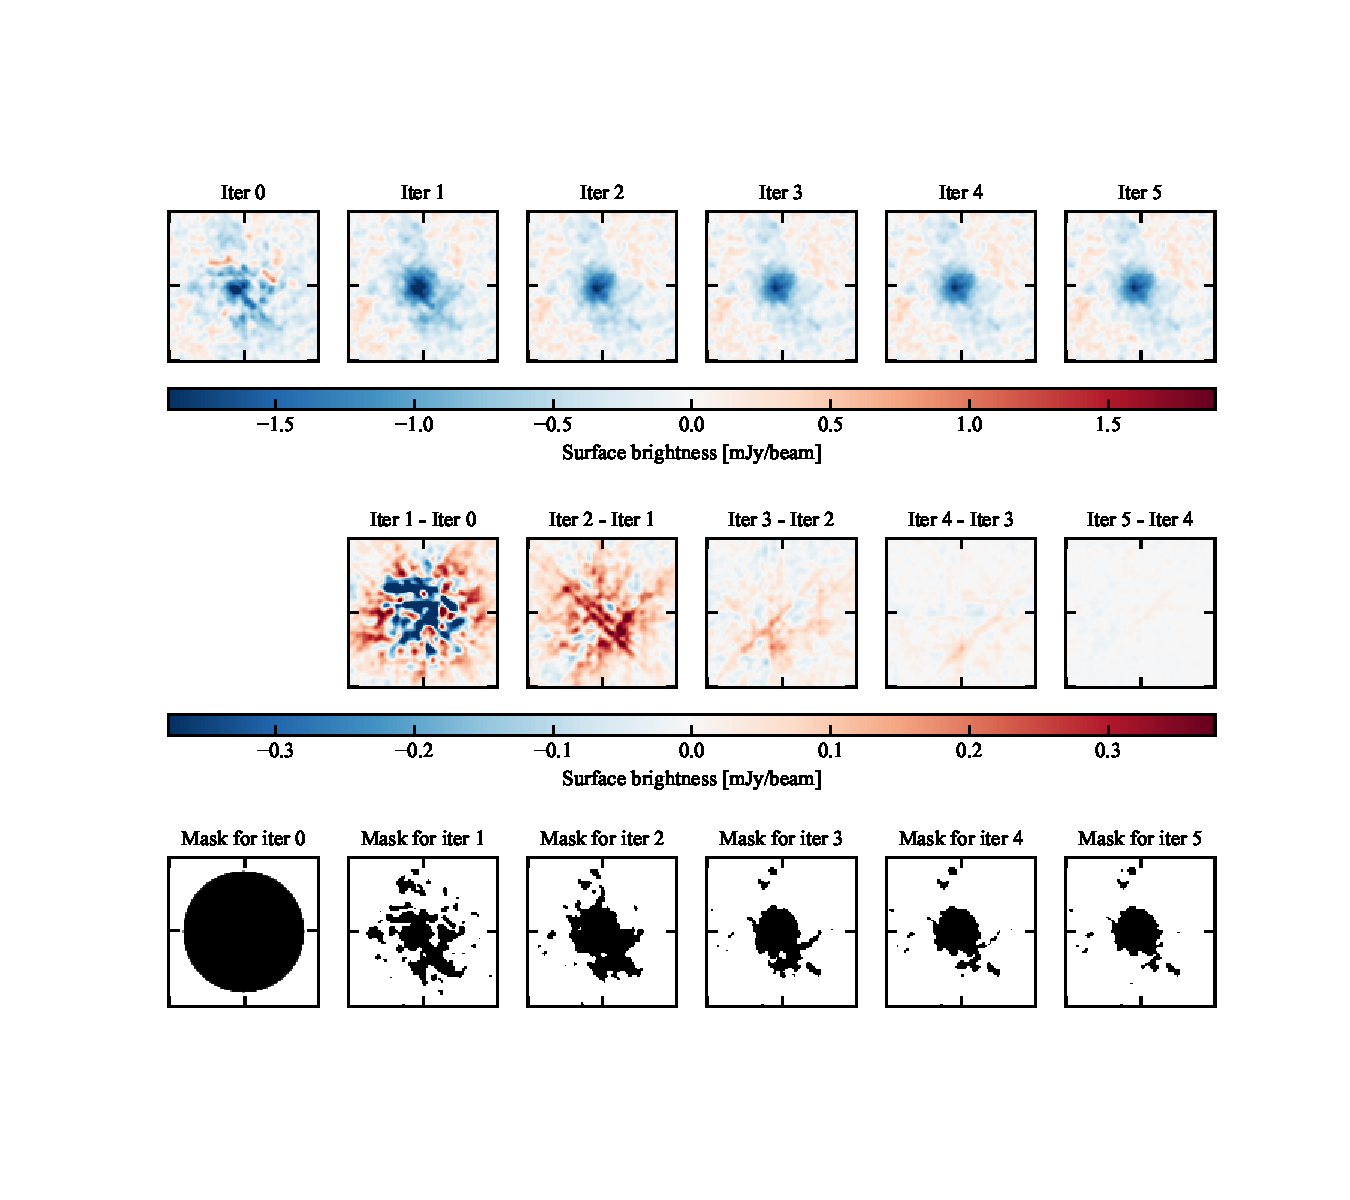
\includegraphics[width=.99\linewidth, trim={2cm 3cm 2cm 3cm}, clip]{Figures/Chap_decor/PSZ2G183_evol_iters.pdf}
    \caption{
        Évolution (de gauche à droite) des résultats avec les itérations de la décorrélation pour les observations NIKA2 de l'amas PSZ2-G183.90+42.99.
        \textbf{Haut:} Carte de brillance de surface obtenue pour chaque itération.
        \textbf{Centre} Différence entre la carte de brillance de surface obtenue pour une itération et pour l'itération précédente.
        \textbf{Bas:} Masque utilisé pour l'évaluation du mode commun pour chaque itération.
    }
    \label{fig:iter_decor}
\end{figure*}

Une décorrélation itérative est illustrée en figure \ref{fig:iter_decor} pour l'amas de galaxies PSZ2-G183.90+42.99.
On voit en haut de la figure, de gauche à droite, l'évolution de la carte de l'amas au fil des itérations.
À partir de la troisième (\guillemotleft Iter 2 \guillemotright), la carte est stable, et n'évolue plus significativement.
Le panneau central montre la différence entre les cartes de deux itérations successives.
On remarque en effet que cette différence converge vers zéro , avec des différences inférieures à $0.1 \;\unit{mJy/beam}$ entre la dernière itération et l'avant-dernière.
Enfin, le panneau bas montre l'évolution du masque utilisé.
On voit que celui-ci mime la morphologie circulaire de l'amas, et que sa forme converge, avec des différences de moins en moins importantes avec les itérations.

% ===================================================================================== %
\section{Des données en temps aux cartes du ciel}\label{sec:projec_toi}

Nous avons vu au cours des sections précédentes comment la procédure de décorrélation permettait d'obtenir des données en temps nettoyées du bruit corrélé, et dominées par le signal d'intérêt.
Il reste donc à projeter ces données pour constituer des cartes du ciel tel qu'observé avec NIKA2.

% ------------------------------------------------------------------------------------- %
\subsection{Projection et cartographie du signal d'intérêt}

La projection utilisée par le \textit{pipeline} de la collaboration NIKA2 est une projection en \textit{nearest grid point}.
Pour cela, une carte de pixels carrés en coordonnées équatoriales et tout d'abord définie.
La taille des pixels est un paramètre de l'analyse, qui peut être choisi.
La taille optimale dépend à la fois de la vitesse de balayage du ciel au cours des observations et de la fréquence d'échantillonnage à laquelle les fréquence des KID sont lues.
En effet, la combinaison de ces deux grandeurs fixe la distance sur le ciel séparant deux échantillons, c'est-à-dire la distance parcourue par le télescope entre deux mesures de fréquence de résonance.
Pour les observations du grand programme SZ de NIKA2, la fréquence d'échantillonnage est $f = 24 \;\unit{Hz}$, et la vitesse de déplacement du télescope de $v = 40 \;\unit{arcsec/s}$.
Le rapport $v/f$ donne donc la distance angulaire séparant deux échantillons consécutifs, qui est de $1.67 \;\unit{arcsec}$.
La taille de pixels est donc choisie comme $3 \;\unit{arcsec}$, permettant à deux échantillons consécutifs de ne jamais être séparés de plus d'un pixel.
%Ce critère assure qu'aucun pixel de la carte ne puisse n'être associée à aucun échantillon. % phrase à double-négation...
Ce critère assure que chaque pixel de la carte soit utilisé pour la projection d'au moins un échantillon.

Une fois la grille de pixels définie, la matrice de pointage $P_k(t, x, y)$ associée à chaque KID est calculée.
La position de chaque détecteur par rapport à un détecteur de référence est connue à chaque instant, comme nous l'avons vu en \mypageref{sec:focal_plane_reconstruction}.
De plus, la position du détecteur de référence dans le ciel étant également connue grâce au pointage du télescope, comme nous l'avons vu en \mypageref{sec:pointing_focus}.
On connait donc, pour chaque mesure de flux réalisée par un KID, la position dans le ciel à laquelle elle a eu lieu.
On peut alors associer chaque mesure de flux au pixel de la carte le plus proche de la position à laquelle elle a été effectuée.

La carte de brillance de surface résultante $I(x, y)$ est obtenue en calculant la moyenne pondérée des mesures associées à chaque pixel:
\begin{equation}
    \label{eq:map_projection}
    I(x, y) = \frac{\sum_{k, t} P_k(t, x, y) \, w_k \; {\rm TOI'}_k(t)}{\sum_{k, t} P_k(t, x, y) \, w_k},
\end{equation}
où ${\rm TOI}'_k(t) = {\rm TOI}_k(t) - B_k(t)$ représente les TOI des détecteurs après soustraction de l'estimation de bruit, c'est-à-dire après la décorrélation. \\
Le poids $w_k$ associé à chaque détecteur $k$ est calculé comme l'inverse de la variance de la TOI du détecteur en dehors du masque $M_k$ (équation \ref{eq:mask_time}).
On a donc:
\begin{equation}
    w_k = \frac{1}{{\rm Var}\,\big[{\rm TOI}_k(t)\big]_{t \,\backslash\, M_k(t) \neq 0}},
\end{equation}
où ${\rm Var}\,[\dots]_{t \,\backslash\, M_k(t) \neq 0}$ représente la variance sur les échantillons $t$ hors du masque, c'est-à-dire la variance hors-source des TOI. \\
Cette pondération permet de donner moins d'importance aux détecteurs dont les données sont toujours fortement bruitées à l'issue de la décorrélation.

% ------------------------------------------------------------------------------------- %
\subsection{Cartes de couverture et de bruit}

Afin de quantifier la couverture des différentes parties du ciel pendant un \textit{scan}, ainsi que le bruit attendu dans les cartes projetées pour ce \textit{scan}, on peut également estimer une carte de couverture et de variance du bruit.
Ces deux cartes sont des sorties naturelles de la procédure de projection.
La carte de couverture, aussi appelée carte de nombre de coups ou de \textit{hits}, représente une cartographie du nombre d'échantillons utilisés pour la projection.
En d'autre termes, il s'agit, pour chaque pixel de la carte, du nombre d'échantillons y ayant été associés par la projection en \textit{nearest grid point}.
Cette carte est obtenue en sommant les matrices de pointages de tous les KID pour tous les échantillons:
\begin{equation}
    \label{}
    N_{\rm hits}(x, y) = \sum_{k, t} P_k(t, x, y).
\end{equation}
Pour un pixel donné, plus ce nombre est élevé, plus le nombre d'échantillons utilisés pour la projection est grand, diminuant ainsi l'incertitude statistique associée au signal en ce point de la carte.

La carte de variance est également un produit de la projection.
En effet, nous avons vu que les échantillons de chaque détecteur étaient pondérés par l'inverse de la variance de sa TOI en dehors de la source.
On peut alors définir une carte de poids, en projetant les poids de chaque détecteur de la même façon que les TOI elles-mêmes sont projetées; ou bien, de façon équivalente, projeter la variance associée à chaque détecteur.
On obtient alors une carte, de pixelisation identique à la carte du signal, représentant la variance des détecteurs utilisés pour la projection du signal dans chaque pixel.
La racine carrée de cette carte donne alors une carte d'écarts-type ou de déviation standard, fournissant une estimation de l'amplitude des fluctuations de bruit, et donc de l'incertitude sur le signal astrophysique en tout point de la carte.

Des exemples de cartes de couverture et de déviation standard de bruit pour un \textit{scan} réalisé au cours des observations de l'amas \act\ dans le grand programme SZ sont présentées dans le panneau haut de la figure \ref{fig:nhits_std_maps}.
On observe la forme rectangulaire des \textit{scans}, caractéristique des observations du grand programme SZ (discutées au paragraphe suivant).
On note également que la carte de couverture montre un nombre plus important de coups dans le centre de la carte qu'en périphérie.
Cette inhomogénéité de couverture s'explique par le fait que plus de détecteurs passent dans les régions du centre de la carte, pour des raisons géométriques, alors que sa périphérie n'est visitée que par un plus faible nombre de KID.
Pour les mêmes raisons, la déviation standard du bruit est plus élevée dans les régions externes de la carte, entraînant des observations de meilleure qualité au centre.
Une analyse détaillée des propriétés de cet amas sera présentée au chapitre \ref{chap:actj0215}.

% ------------------------------------------------------------------------------------- %
\subsection{Coaddition de cartes} \label{sec:map_coadd}

Tout comme la carte de brillance de surface associée à un \textit{scan} est calculée par une moyenne pondérée des signaux reçus par les KID, la combinaison de plusieurs \textit{scans} permet de construire une carte de brillance de surface en calculant la moyenne pondérée des cartes de ces derniers.
La carte de brillance résultant de la combinaison de $n$ \textit{scans}, donc les cartes de brillance de surface individuelles $I_s(x,y)$ sont calculées par l'équation (\ref{eq:map_projection}), est donnée par:
\begin{equation}
    \label{eq:map_coadd}
    I_{\rm tot}(x, y) = \frac{\sum_{s=1}^{n} w_s(x, y) \, I_s(x, y)}{\sum_{s=1}^{n} w_s(x, y)},
\end{equation}
où les poids $w_s(x, y)$ sont définis pour chaque carte à partir de la carte de couverture $N_{\rm hits}(x, y)$ et de la variance de la carte de brillance de surface en dehors du masque de la source:
\begin{equation}
    \label{eq:coadd_weights}
    w_s(x, y) = \frac{N_{{\rm hits}, s}(x, y)}{V \, \big[ I_s(x, y) \times \sqrt{N_{{\rm hits}, s}(x, y)} \big]_{(x, y) \,\backslash\, M(x, y) \neq 0}}.
\end{equation}
Tout comme la pondération par la variance des TOI nous a permis de donner moins d'importance aux détecteurs bruités, cette pondération permet de donner moins d'importance dans la carte finale aux \textit{scans} dans lesquels le bruit est toujours important après la décorrélation.
Le terme $\sqrt{N_{{\rm hits}, s}(x, y)}$ au dénominateur permet de normaliser la carte au temps passé par pixel.

Nous avons vu au chapitre précédent que la stratégie de \textit{scan} utilisée pour les observations du grand programme SZ de NIKA2 était basée sur une succession de groupes de quatre \textit{scans}, réalisés à des angles de $0$\textdegree, $45$\textdegree, $90$\textdegree, et $135$\textdegree par rapport à l'axe des ascensions droites.
La procédure de coaddition est donc particulièrement importante dans ce contexte.
Le panneau bas de la figure \ref{fig:nhits_std_maps} montre les cartes de couverture et de déviation standard du bruit obtenues par coaddition de quatre \textit{scans} de l'amas \act, dont celui présenté dans le panneau haut de la figure.
Les observations faites sur le panneau haut (voir section précédente) restent valides: le centre de la carte bénéficie d'une meilleure couverture, et donc d'une déviation standard de bruit plus faible.
On voit également que la combinaison de \textit{scans} dans quatre angles différents a eu pour effet d'augmenter la couverture dans la carte (puisqu'on considère quatre \textit{scans} au lieu d'un seul), mais également de la rentre plus isotrope.
De même, le bruit dans la carte coadditionnée est plus bas, et reste bas dans une grande région à symétrie circulaire.
C'est là l'objectif de l'utilisation de \textit{scans} dans plusieurs directions mise en place pour les observations du grand programme SZ de NIKA2, en plus de l'optimisation du filtrage, que nous discuterons en section \mypageref{sec:transfer_function}.

\begin{figure*}[t]
    \centering
    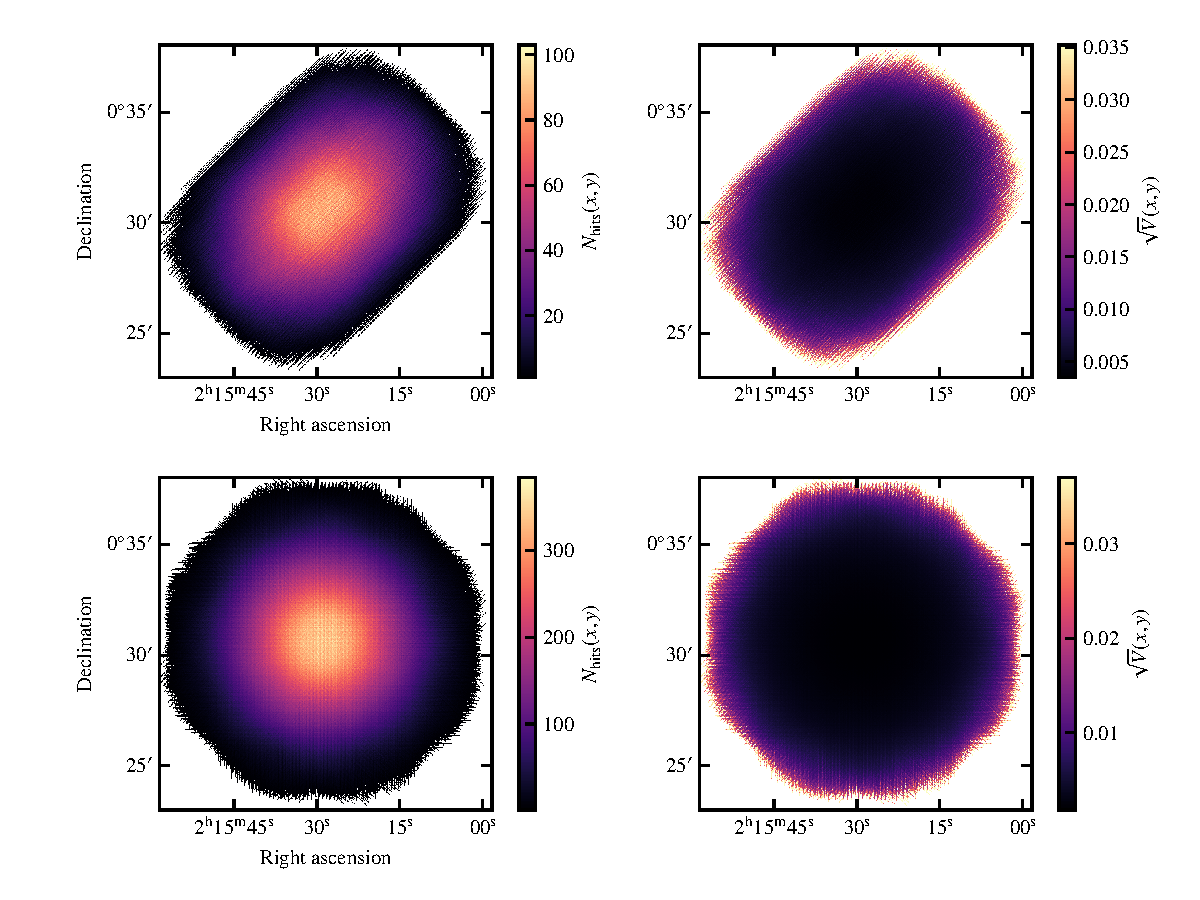
\includegraphics[width=\linewidth]{Figures/Chap_decor/scans.pdf}
    \caption{
        \textbf{Haut:} carte de couverture (\textit{gauche}) et de déviation standard du bruit (\textit{droite}) à 150 GHz pour un \textit{scan} du grand programme SZ de NIKA2.
        \textbf{Bas:} Même cartes pour la combinaison de quatre \textit{scans} dans quatre orientations différentes, incluant le \textit{scan} du panneau haut.
    }
    \label{fig:nhits_std_maps}
\end{figure*}

% ===================================================================================== %
\section{Performance de la décorrélation}\label{sec:perf_decor}

Quelle que soit la méthode choisie pour la procédure de décorrélation, celle-ci est toujours imparfaite.
Nous avons vu que la décorrélation avait deux objectifs, qui sont de retirer un maximum de bruit corrélé des données en temps sans porter atteinte au signal astrophysique d'intérêt.
Par conséquent, on quantifie la performance de la procédure au travers de critères évaluant l'atteinte de ces deux objectifs: le bruit corrélé résiduel, et le filtrage du signal.
Ces deux quantités seront ensuite utilisées au cours de l'analyse des données de NIKA2 afin de tenir compte des caractéristiques de la décorrélation.

% ------------------------------------------------------------------------------------- %
\subsection{Bruit corrélé résiduel}\label{sec:noise_pk}

À l'issue de la procédure de décorrélation, une partie du bruit reste inévitablement présente dans les données en temps.
Nous avons vu précédemment qu'une partie de ce bruit était le bruit blanc intrinsèque à chaque détecteur, ne pouvant par nature pas être soustrait des données en temps.
En réalité, une partie du bruit corrélé dû à l'atmosphère et à l'électronique reste également présent.
La présence de ce bruit corrélé résiduel est donc une indication de l'imperfection de la méthode de décorrélation.
Puisque ce bruit reste dans les données en temps après la décorrélation, il est projeté dans les cartes de brillance de surface au même titre que le signal astrophysique.
De plus, puisqu'il est corrélé, il peut faire apparaître des structures de bruit dans les cartes, pouvant être faussement interprétées comme du signal d'intérêt.
Il est donc important de connaitre le comportement de ce bruit en vue de la mesure des propriétés des amas de galaxies à partir des observations avec NIKA2.

L'information pertinente sur le bruit corrélé résiduel est présente dans son spectre de puissance.
L'évaluation de celui-ci ne peut pas avoir lieu directement dans les données NNIKA2, puisque celles-ci contiennent également du signal d'intérêt.
Cependant, il est possible d'utiliser les cartes de demi-différences entre les \textit{scans}.
Pour cela, on réalise la coaddition des $n$ cartes des différents \textit{scans} d'après:
\begin{equation}
    I'(x, y) = \frac{\sum_{s=1}^{n} w_s(x, y) \, I_s(x, y) \times (-1)^s}{\sum_{s=1}^{n} w_s(x, y)},
\end{equation}
où les poids $w_s$ sont les mêmes que pour la coaddition des \textit{scans}, calculés par l'équation (\ref{eq:coadd_weights}). \\
Ainsi, la carte d'un \textit{scan} sur deux se voit multipliée par $(-1)$ dans la coaddition.
Puisque le signal astrophysique est \prior\ la seule composante des cartes constante d'un \textit{scan} à l'autre, il est complètement annulé\footnotemark\ dans la carte $I'(x, y)$.
En revanche, le bruit corrélé pouvant indifféremment être positif ou négatif, sa structure n'est pas modifiée au cours de l'opération.
\footnotetext{On note la nécessité d'un nombre pair de \textit{scans} dans cette procédure, sans quoi le signal ne peut complètement s'annuler.
De même, il est nécessaire d'ordonner les \textit{scans} par angle lors de la coaddition, afin de ne pas systématiquement ajouter ou soustraire les cartes obtenues à un angle donné, ce qui crée des structures de bruit différentes.}
On obtient ainsi une carte, vide de tout signal d'intérêt, contenant seulement du bruit dont les propriétés sont les mêmes que celles du bruit présent dans la carte de signal obtenue par coaddition.

Le spectre de puissance du bruit résiduel est calculé sur la carte de demi-différences, normalisée par la carte de déviation standard du bruit:
\begin{equation}
    \label{eq:noise_power_spectrum}
    P_{\rm bruit}(k) = \left| \, F \left( \frac{I'(x, y)}{\sqrt{V}(x, y)} \right) \, \right|^2,
\end{equation}
où $F$ représente l'opération de transformée de Fourier. \\
Cette normalisation permet de tenir compte de la plus grande amplitude de bruit attendue dans les bords des cartes, du fait de la couverture plus faible dans ces régions.
La forme du spectre de puissance nous renseigne sur la corrélation du bruit résiduel.
Si ce dernier est blanc, c'est-à-dire ne présente pas de corrélations résiduelles, son spectre de puissance doit être plat.
À l'inverse, le spectre de puissance d'un bruit fortement corrélé à grande échelle se manifeste comme une fonction en loi de puissance, $P(k) \propto k^{-\alpha}$.
Pour la décorrélation \textit{common mode one block} réalisée sur les amas du grand programme SZ, c'est ce dernier comportement qui est observé.
Nous verrons par exemple au chapitre \ref{chap:actj0215} que le bruit résiduel dans les observations de l'amas \act\ est très corrélé, comme en atteste le spectre de puissance présenté en figure \ref{fig:act:tf_noise}.

C'est pourquoi la présence de bruit corrélé doit être prise en compte au cours des exploitations des observations d'amas de galaxies par NIKA2.
Nous verrons au chapitre suivant que cette prise en compte est possible au travers de la matrice de covariance du bruit résiduel.
Celle ci peut être calculée à partir du spectre de puissance comme suit:
\begin{enumerate}[leftmargin=*]
    \item Un grand nombre ($N \sim 10^5$) de cartes de bruit blanc est généré.
        Dans chacune des cartes, chaque pixel est tiré aléatoirement dans une distribution gaussienne de moyenne $0$ et de variance $1$.
    \item Chacune de ces cartes est convoluée par le spectre de puissance du bruit calculé par l'équation (\ref{eq:noise_power_spectrum}).
        Les cartes résultantes sont des réalisations de bruit normalisées suivant le spectre de puissance d'entrée.
    \item Chacune des cartes est ensuite multipliée par la carte de déviation standard du bruit $\sqrt{V}(x, y)$.
        Les cartes résultantes sont des réalisations de bruit résiduel dont l'amplitude et les corrélations sont les mêmes que dans la carte de demi-différences.
        Chaque carte, de dimension $(n \times n)$, est déroulée en un vecteur de dimension $(n^2 \times 1)$.
    \item La matrice de covariance des $N$ vecteurs est calculée.
\end{enumerate}
Pour une carte d'entrée de dimensions $(n \times n)$ pixels, le résultat est une matrice de taille $(n^2 \times n^2)$, dans laquelle chaque élément $(i, j)$ représente la covariance du bruit dans les pixels $i$ et $j$ de la carte.
Nous verrons au chapitre suivant que c'est cette matrice qui est utilisée dans la fonction de vraisemblance multivariée de l'ajustement des données NIKA2 par un modèle de propriétés physiques du milieu intra-amas, afin de tenir compte de la corrélation du bruit résiduel.
Elle sera utilisée au travers d'une fonction de vraisemblance gaussienne multivariée, discutée en section \mypageref{sec:panco:likelihood}.

\begin{figure*}[t]
    \centering
    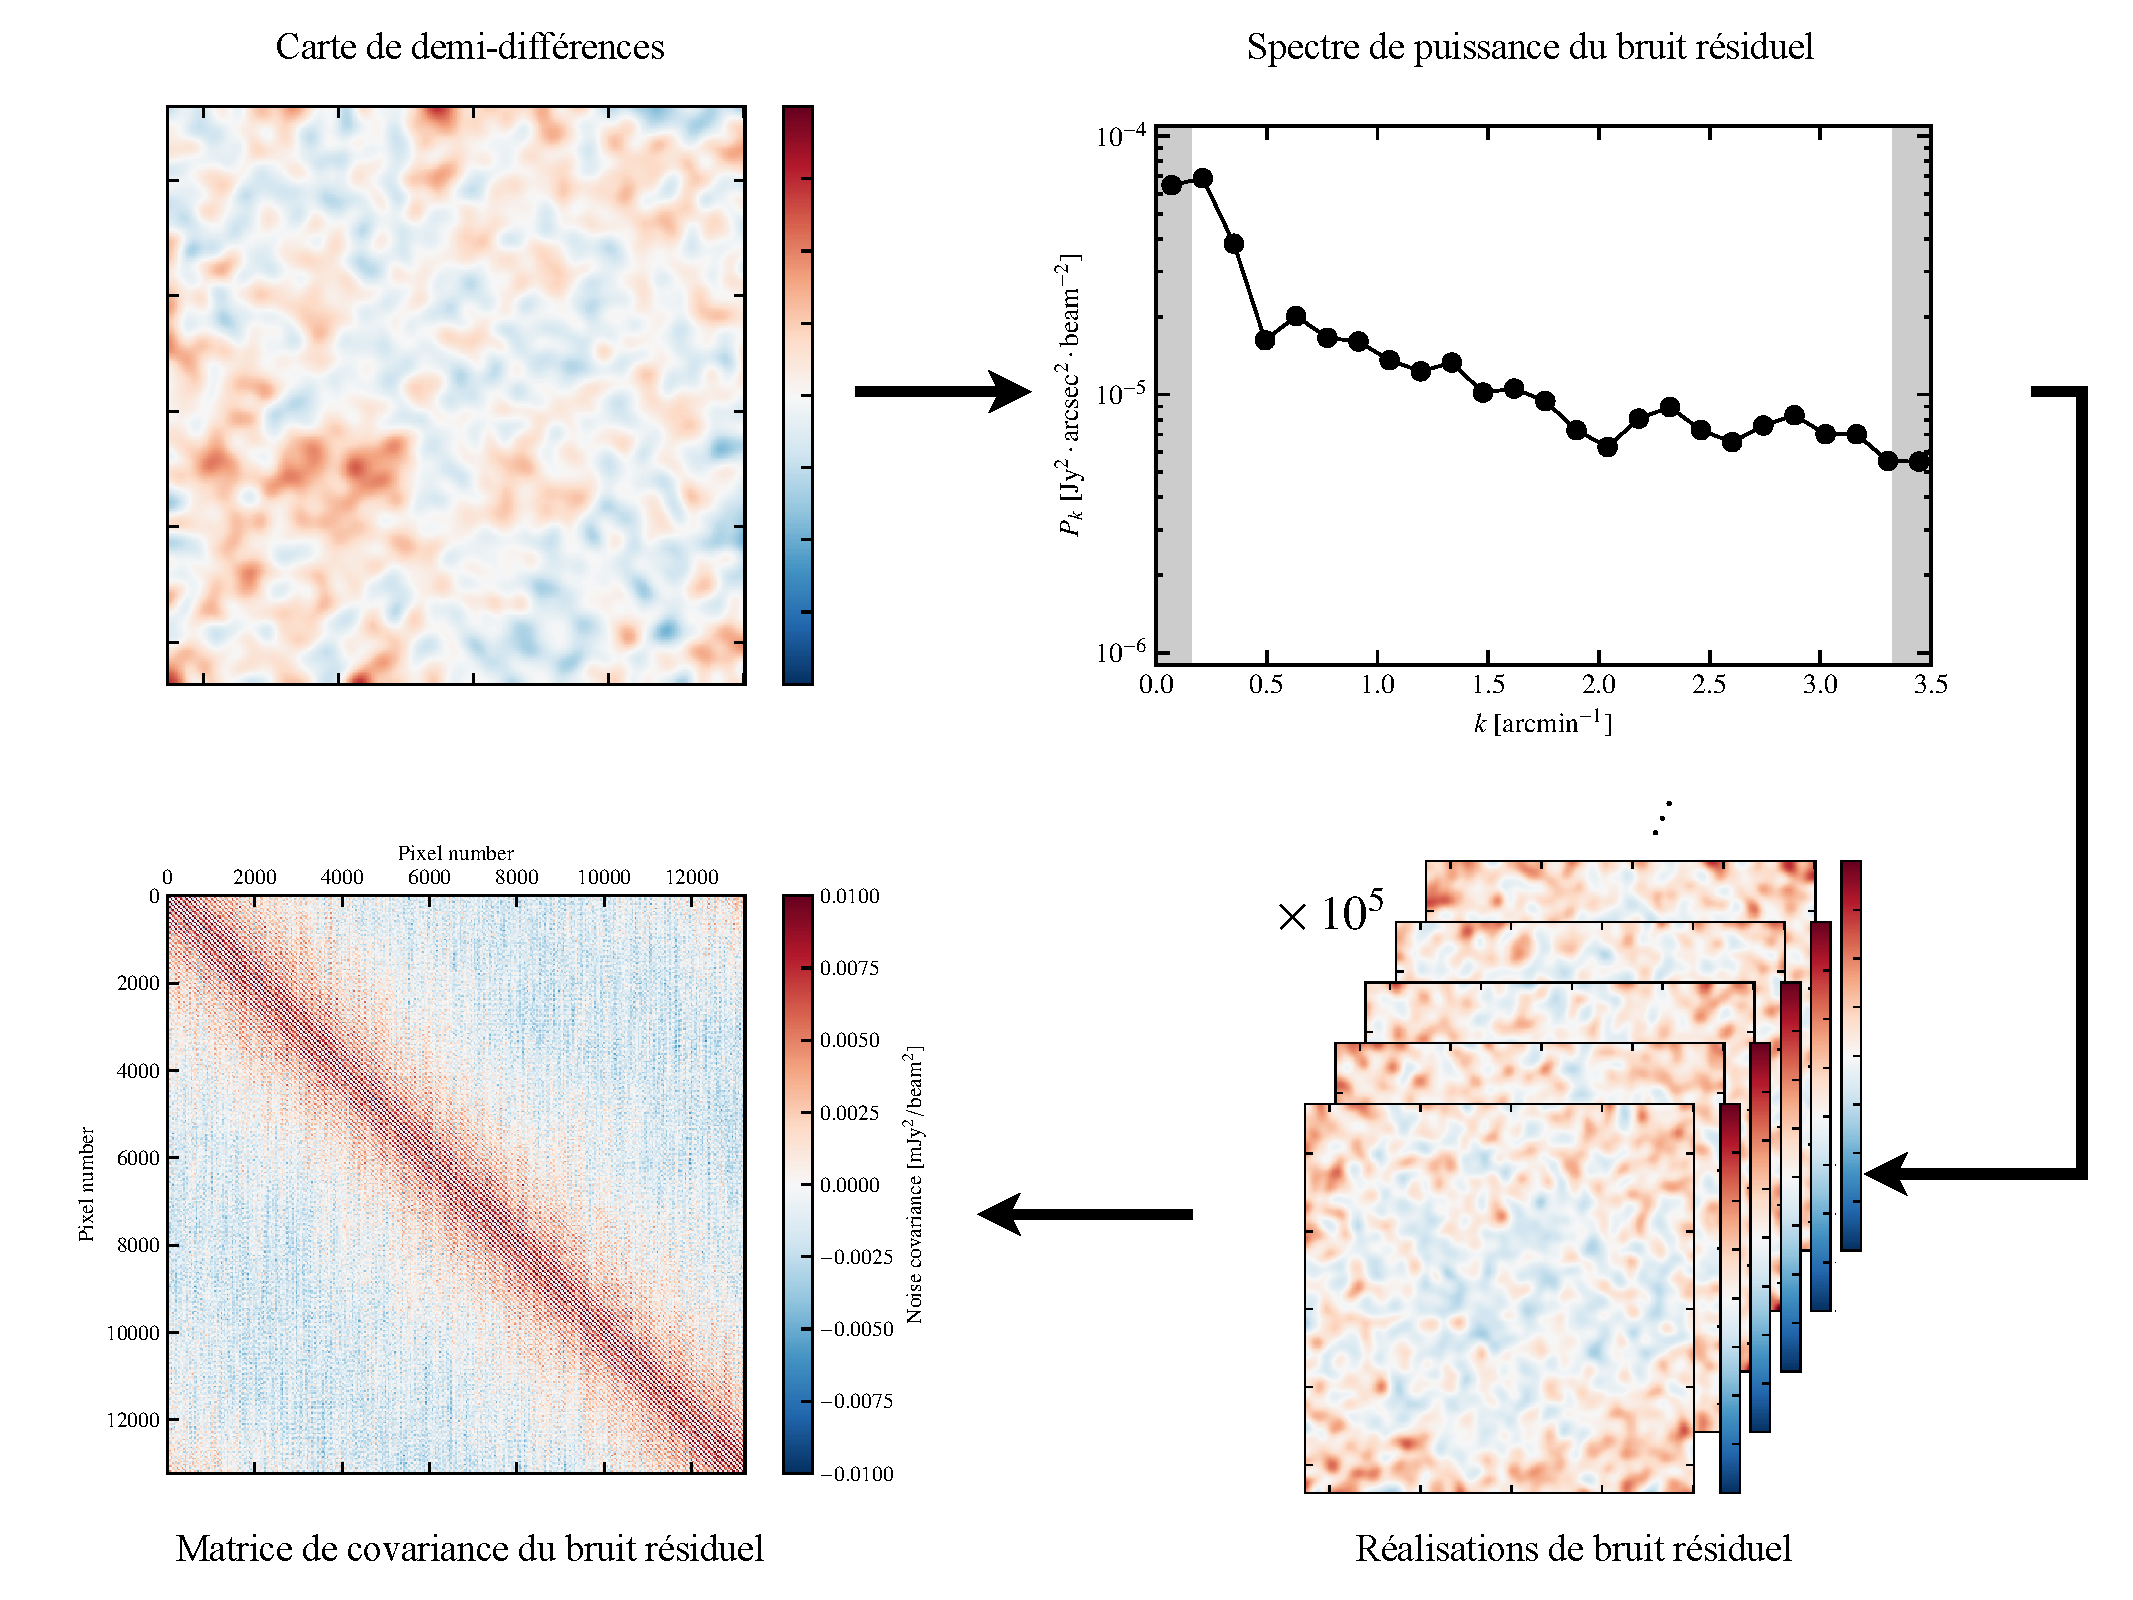
\includegraphics[width=.99\linewidth, page=1]{Figures/Chap_decor/schema_pk_tf.pdf}
    \caption{
        Illustration du calcul de la matrice de covariance du bruit résiduel pour la décorrélation \textit{common mode one block} de l'amas PSZ2-G183.90+42.99 (voir figure \ref{fig:iter_decor}).
        La carte de demi-différences (\textit{haut gauche}) est utilisée pour calculer le spectre de puissance du bruit résiduel (\textit{haut droit}), à son tour utilisé pour générer des réalisations de bruit corrélé de même spectre de puissance (\textit{bas droit}).
        La covariance de ces réalisations donne la matrice de covariance pixel-à-pixel du bruit résiduel (\textit{bas gauche}).
    }
    \label{fig:noise_pk_schema}
\end{figure*}

La procédure d'estimation du bruit résiduel et de sa matrice de covariance est présentée en figure \ref{fig:noise_pk_schema}.
Le cas choisi pour l'illustration est la décorrélation \textit{common mode one block} des observations de l'amas PSZ2-G183.90+42.99, dont le processus itératif est représenté en figure \ref{fig:iter_decor}.
Le spectre de puissance du bruit résiduel (haut droite de la figure) n'est pas plat, indiquant un bruit résiduel corrélé à grande échelle.
Par conséquent, la matrice de covariance du bruit (bas gauche) n'est pas diagonale.
Dans le cas où le bruit résiduel est proche d'un bruit blanc, les corrélations du bruit entre deux pixels différents de la carte sont faibles, et les éléments extra-diagonaux de la matrice de covariance sont négligeables.
Ce comportement traduirait une décorrélation parfaite.
De plus, comme nous le verrons au chapitre suivant, ce comportement est idéal, car il permet de ne pas tenir compte de la matrice de covariance du bruit lors de l'ajustement des propriétés des amas à partir des observations NIKA2, ce qui accélère grandement le processus.

% ------------------------------------------------------------------------------------- %
\subsection{Filtrage du signal}\label{sec:transfer_function}

Si la décorrélation ne permet pas de retirer complètement le bruit corrélé des données en temps, elle est aussi imparfaite du point de vue de la conservation du signal.
En effet, nous avons vu en section \ref{sec:mask_decor} que le masque utilisé pour éviter le biais dû au signal dans l'estimation du mode commun était défini comme la région du ciel dans laquelle le rapport signal sur bruit était supérieur à $3\sigma$.
Par construction, tout signal moins significatif n'est pas protégé par ce masque, et peut être inclus dans le mode commun.
Il est alors soustrait comme du bruit, ce qui induit un filtrage du signal d'intérêt.
Par ailleurs, nous avons vu que le masque était défini de façon itérative, en commençant avec un masque circulaire assez grand pour englober le signal.
Il ne s'agit toutefois pas simplement de définir un masque le plus grand possible pour masquer une grande portion de la carte, puisqu'une couverture du ciel minime entraînera un mode commun estimé sur peu de détecteurs, et donc potentiellement une mauvaise estimation de bruit.
Ces défauts sont donc d'autant plus importants que la source observée est spatialement étendue.
Les amas de galaxies observés dans le cadre du grand programme SZ de NIKA2 étant grands devant le lobe de l'instrument (voir section \ref{sec:lpsz}), ils sont affectés par ce filtrage.
Il est donc nécessaire de connaitre les propriétés de ce filtrage, afin de pouvoir faire le lien entre le signal SZ réel associé à l'amas et le signal détecté, faute de quoi les propriétés physiques mesurées seront biaisées.

Ce filtrage est estimé par la fonction de transfert de l'analyse.
Celle-ci est évaluée par la mesure du filtrage subi par un signal connu lorsque celui-ci est soumis à la procédure de décorrélation.
Pour l'analyse des données associées à un amas, une fois la décorrélation terminée, une carte de l'effet SZ dû à l'amas est simulée par intégration d'un profil de pression universel le long de la ligne de visée.
Cette carte est projetée sur la même grille pixélisée que la carte de brillance de surface NIKA2.
Une réalisation de bruit blanc, d'amplitude largement inférieure au signal SZ simulé, est ajoutée à la carte afin d'éviter la présence de zéros dans la carte et dans son spectre de puissance.
L'importante de ce bruit sera discutée par la suite.
La carte simulée obtenue $S_{\rm in.}$ est ensuite convertie en données en temps pour chaque détecteur grâce à la matrice de pointage de ces derniers.
Les données en temps ainsi obtenues, entièrement dominées par le signal simulé, sont ajoutées aux données réelles.
Cette somme forme donc des TOI pour chaque détecteur contenant les différents contaminants caractéristiques des observations avec NIKA2, le signal astrophysique d'intérêt, et le signal simulé.

Les données en temps ainsi obtenues sont soumises à la même procédure de décorrélation que les données NIKA2 ne contenant pas le signal simulé.
La procédure itérative n'est pas nécessaire, puisqu'elle vise seulement à définir le masque le plus adapté à la protection du signal d'intérêt.
Ainsi, la procédure de décorrélation est réalisée sur les TOI contenant le signal simulé en considérant le masque utilisé pour la dernière itération de la décorrélation des données brutes.
De cette façon, le traitement subi par les données contenant le signal simulé est identique à celui subi par les données brutes.
On peut donc supposer que le filtrage subi par le signal simulé est identique à celui subi par le signal astrophysique d'intérêt.

La carte de signal simulé reconstruit $S_{\rm out.}$ est ensuite calculé comme la différence entre la carte issue de la décorrélation des données en temps contenant le signal simulé et celle issue de la décorrélation des données brutes (ne contenant pas de signal simulé).
La fonction de transfert de l'analyse ${\rm TF}(k)$, quantifiant le filtrage subi par le signal simulé, est calculée comme le rapport entre les spectres de puissance des cartes de signal simulé avant et après la décorrélation:
\begin{equation}
    \label{eq:transfer_function}
    {\rm TF}(k) = \frac{\big| F(S_{\rm out.}) \big|^2}{\big| F(S_{\rm in.}) \big|^2}
\end{equation}
Puisque le processus subi par le signal simulé est identique à celui subi par le signal astrophysique d'intérêt, cette fonction de transfert représente un bon estimateur du filtrage subi par ce dernier au cours de la décorrélation ne contenant pas de signal simulé.
L'intérêt de l'ajout de bruit blanc dans la carte de signal simulé $S_{\rm in.}$ apparaît clairement dans l'équation (\ref{eq:transfer_function}).
Si cette étape n'était pas réalisée, il existe un risque que le spectre de puissance de la carte présente des zéros.
Ce dernier étant au dénominateur de l'équation (\ref{eq:transfer_function}), la fonction de transfert peut diverger.
%L'analyse des données de l'amas \act\ présentée au chapitre \ref{chap:actj0215} présentera la fonction de transfert obtenue pour la décorrélation des données de cet amas en utilisant la méthode \textit{common mode one block}, montrée en figure \ref{fig:act:tf_noise}.

\begin{figure*}[t]
    \centering
    \includegraphics[width=.99\linewidth, page=2]{Figures/Chap_decor/schema_pk_tf.pdf}
    \caption{
        Illustration du calcul de la fonction de transfert pour la décorrélation \textit{common mode one block} de l'amas PSZ2-G183.90+42.99 (voir figure \ref{fig:iter_decor}).
        Le rapport entre les spectres de puissance d'une carte simulée d'entrée ($S_{\rm in.}$, \textit{haut}) et de la carte après décorrélation ($S_{\rm out.}$, \textit{bas}) donne la fonction de transfert de la décorrélation.
    }
    \label{fig:tf_schema}
\end{figure*}

Le processus d'estimation de la fonction de transfert pour la décorrélation des observations de l'amas PSZ2-G183.90+42.99 est schématisé en figure \ref{fig:tf_schema}.
La fonction de transfert résultante, représentée à droite de la figure, est caractéristiques de la décorrélation \textit{common mode one block} des observations NIKA2 d'amas de galaxies.
Elle est caractérisée par un filtrage des grandes échelles angulaires ($k < 0.5 \;\unit{arcmin^{-1}}$), résultant en une suppression quasi-totale du signal aux échelles plus grandes que le champ de vue instantané de NIKA2 ($6.5 \;\unit{arcmin}$), représentées par la région grisée à gauche de la figure.
En revanche, les échelles angulaires plus petites sont bien conservées, avec un filtrage proche de $1$.
Nous verrons dans le chapitre suivant que cette fonction de transfert est utilisée lors de la mesure des propriétés thermodynamiques du milieu intra-amas à partir des observations NIKA2 des amas du grand programme SZ, afin de tenir compte du filtrage induit par la décorrélation.

% ===================================================================================== %
\section{Contamination par des sources ponctuelles}
\label{sec:decor:pstools}

Nous avons vu au chapitre \ref{chap:nika2} que l'effet SZ pouvait être mesuré avec NIKA2 par le décrément en brillance de surface dans la carte à 150 GHz.
Ce signal peut être affecté par des sources ponctuelles, de flux positif qui compense partiellement ou totalement le décrément.
Afin d'obtenir des contraintes non-biaisées sur le signal SZ d'un amas -- et donc sur ses propriétés thermodynamiques -- il est donc nécessaire de traiter cette contamination en estimant le flux des sources.
Celui-ci ne peut par construction pas être mesuré directement dans la carte NIKA2 à 150 GHz, puisqu'il est dégénéré avec le décrément SZ inconnu.
Il est donc nécessaire de s'appuyer sur des données externes.

Un estimateur du flux d'une source est donné par l'évolution de son émission avec la fréquence d'observation, qui est quantifiée par son spectre (SED, pour \textit{Spectral Energy Distribution}).
Le logiciel \texttt{PSTools} a été développé dans le cadre de cette thèse, et permet d'ajuster ce flux pour des sources sub-millimétriques à partir d'un catalogue de sources et des données NIKA2.
Ce logiciel a été documenté \cite{keruzore_pstools_2019} et mis à disposition de la collaboration NIKA2, devenant l'outil principal d'estimation de la contamination des cartes SZ obtenues avec NIKA2 par des sources sub-millimétriques.
Cette section décrit la procédure employée et implémentée dans \texttt{PSTools}; son utilisation dans le cadre de l'analyse des propriétés de l'amas \act\ sera présentée au chapitre \ref{chap:actj0215}.

% ------------------------------------------------------------------------------------- %
\subsection{Données d'entrée}

Les sources ponctuelles contaminant le signal SZ peuvent être des sources d'avant plan, d'arrière plan, ou même des galaxies membres de l'amas.
Dans tous les cas, ces sources peuvent être classifiées en deux catégories.
D'une part, elle peuvent être des galaxies poussiéreuses émettant dans le domaine sub-millimétrique (SMG pour \textit{submillimeter galaxies}), avec un flux croissant avec la fréquence dans le domaine couvert par les observations NIKA2.
Elles peuvent également être des sources radio, présentant une émission plus forte à basse fréquence\footnotemark.
\footnotetext{Notons que cette distinction entre galaxie poussiéreuse et source radio est une simplification, le spectre d'émission de la poussière présentant une composante d'émission radio.}
Les SMG sont plus simples à identifier avec NIKA2, puisque leur flux est plus élevé dans la bande à 260 GHz, où le signal SZ n'est en général pas détectable.

Afin de mesurer le spectre d'une source, la connaissance du flux des sources dans une large gamme de fréquence est nécessaire.
\texttt{PSTools} permet de traiter la contamination due à des sources submillimétriques détectées par l'instrument SPIRE à bord du satellite \textit{Herschel} \cite{griffin_herschel-spire_2010}.
Nous utilisons la combinaison des mesures des flux dans chacune des bandes de SPIRE (250, 350, et 500 $\mu$m, soit 1200, 860, et 600 GHz, respectivement) et dans la bande à 260 GHz de NIKA2, dans laquelle le signal SZ est négligeable devant le bruit et le flux des sources ponctuelles.
Il est également possible d'utiliser les flux des sources à plus haute fréquence dans les bandes passantes de l'instrument PACS à bord de \textit{Herschel} \cite{poglitsch_photodetector_2010}, lorsque ceux-ci sont publics.
Par la suite, nous considèrerons le cas où seules des données SPIRE sont disponibles, cas bien plus fréquent pour les amas du grand programme SZ.

Un schéma du fonctionnement de \texttt{PSTools} est présenté en figure \ref{fig:pstools_schema}.
Les données d'entrée sont donc un catalogue de sources avec leurs positions et flux dans les trois bandes de SPIRE d'une part, et les données NIKA2 à 260 GHz d'autre part, incluant la carte de signal, de bruit, et la fonction de transfert associée.
Dans la suite, nous présentons les trois grandes étapes de l'analyse, représentées en bleu-vert sur la figure \ref{fig:pstools_schema}, et les illustrons pour des sources considérées dans l'analyse de l'amas \act, présentée au chapitre \ref{chap:actj0215}.

\begin{figure*}[t]
    \centering
    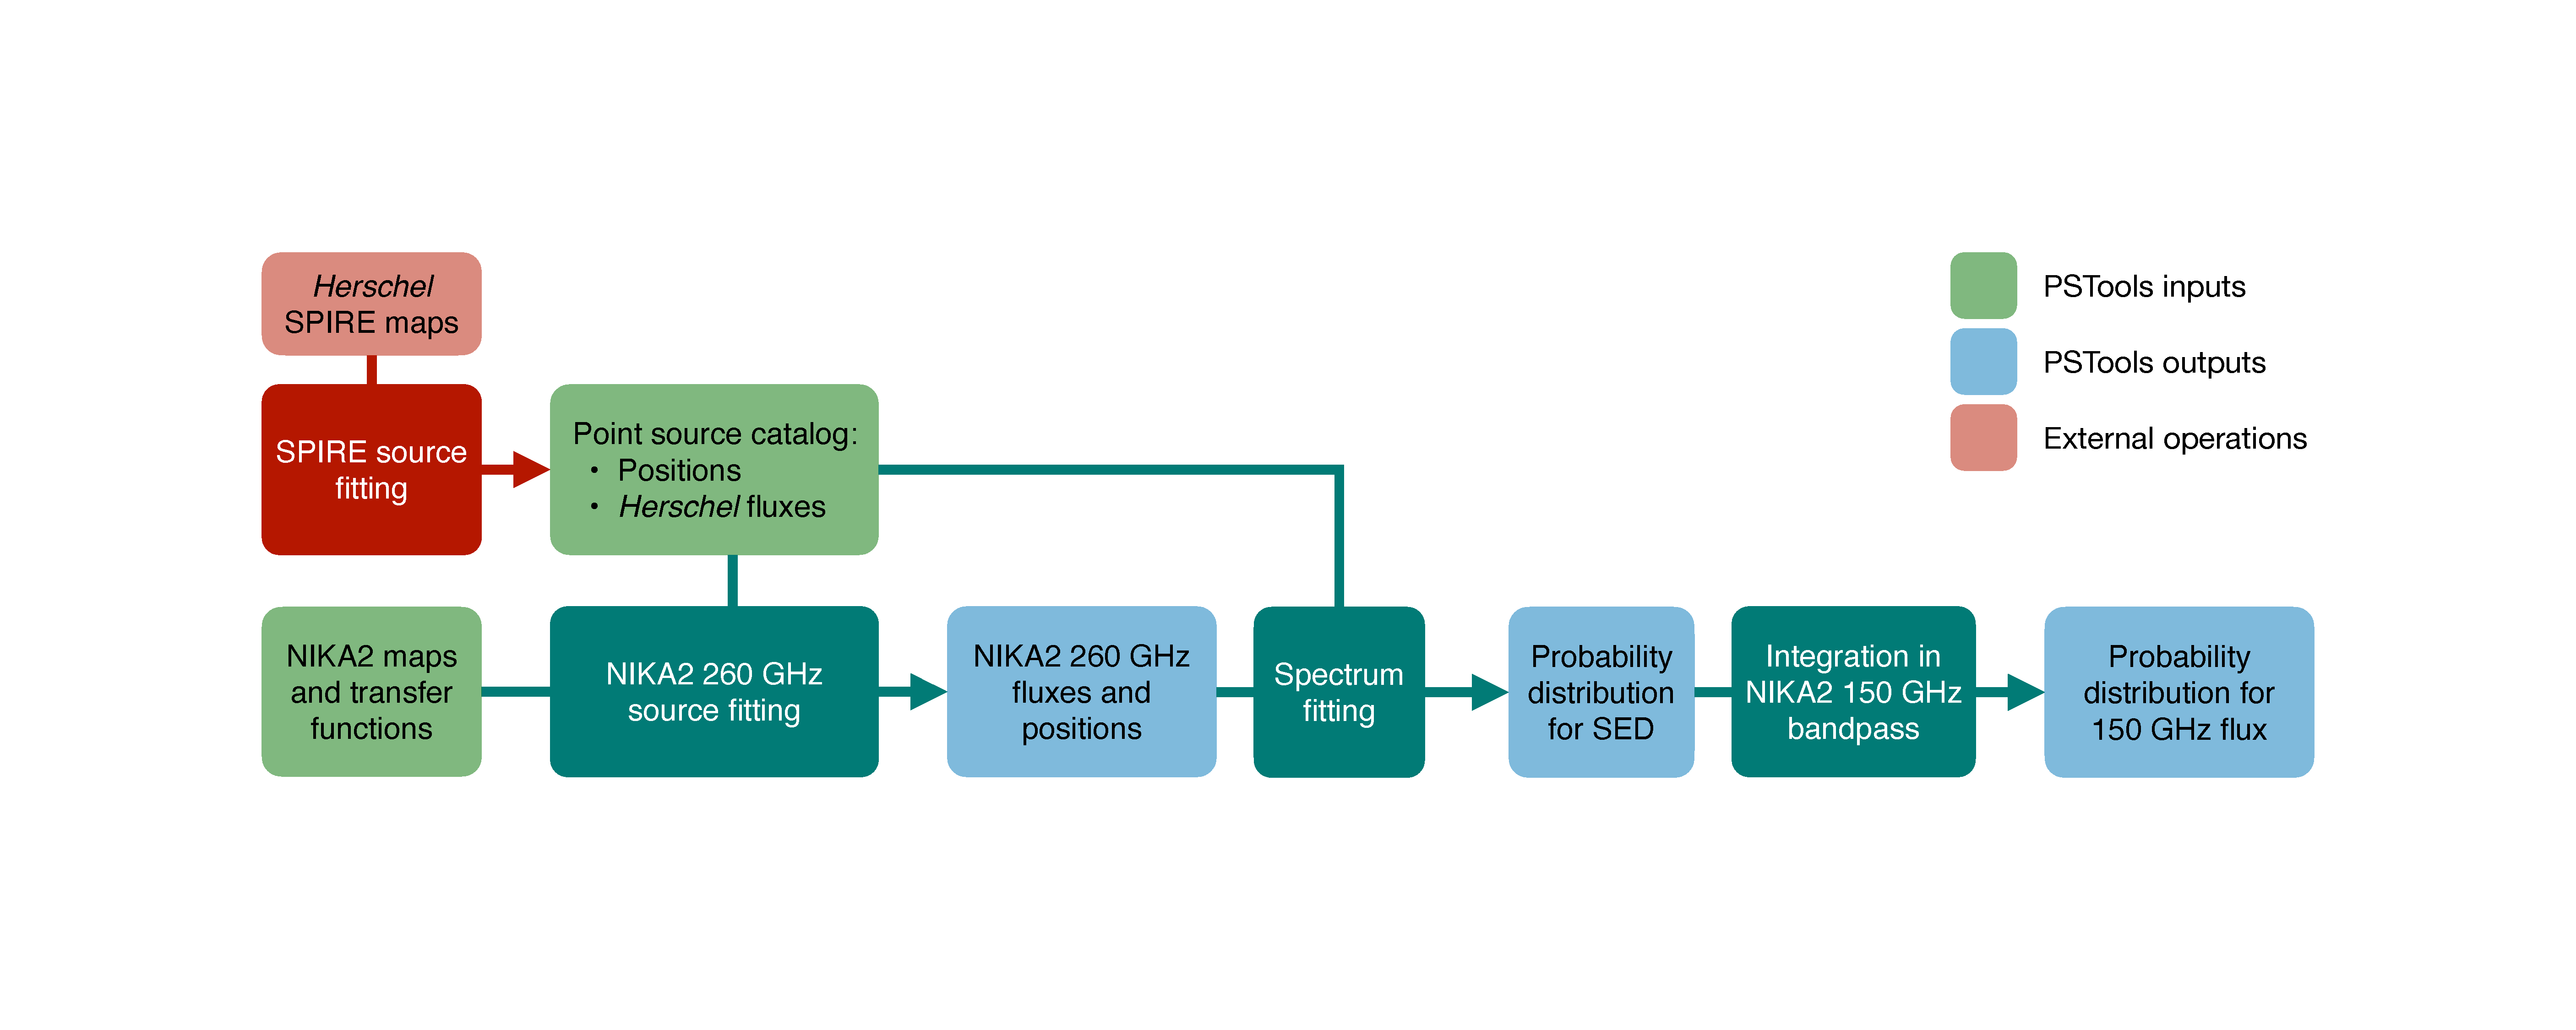
\includegraphics[width=\linewidth, trim={8cm, 7cm, 8cm, 7cm}, clip]{Figures/Chap_decor/PSTools.pdf}
    \caption{
        Schéma illustrant le fonctionnement de \texttt{PSTools}.
        Les données d'entrée sont représentées en vert, et les données de sortie en bleu.
        La partie rouge représente les opérations externes au logiciel, c'est-à-dire la détection des sources dans les cartes SPIRE.
    }
    \label{fig:pstools_schema}
\end{figure*}

% ------------------------------------------------------------------------------------- %
\subsection{Mesures de coordonnées et flux à 260 GHz}

Le flux de chaque source à 260 GHz et sa position sont mesurés dans la carte NIKA2 à cette fréquence.
Pour cela, un modèle de lobe de NIKA2 est ajusté dans une portion carrée de la carte, centrée sur la position de détection de chaque source dans SPIRE.
L'évolution de la mesure du flux des sources avec la taille de cette portion a été étudiée, montrant de meilleurs résultats pour des tailles de l'ordre de 1'.
Le lobe est modélisé par une Gaussienne de largeur à mi-hauteur fixée à $\mathrm{FWHM} = 12.5$'', en accord avec le modèle utilisé pour l'étalonnage des cartes \cite{perotto_calibration_2020}, avec une amplitude et une position libres, ainsi qu'un éventuel niveau zéro.
L'ajustement est réalisé à l'aide de la librairie Python \texttt{iminuit} \cite{hans_dembinski_scikit-hepiminuit_2020}, et l'amplitude de la Gaussienne ajustée livre une estimation du flux de la source à 260 GHz.
Lorsque deux sources sont proches, elles sont ajustées simultanément dans la même portion de carte, afin d'éviter une surestimation des flux.
Un exemple d'ajustement est présenté en figure \ref{fig:pstools_1mm} pour une source simple et un ensemble de deux sources proches, montrant les données, le meilleur ajustement, et la différence entre les deux cartes.
On voit que cette différence ne présente pas de structure au niveau des sources, indiquant un ajustement correct.

\begin{figure*}[t]
    \centering
    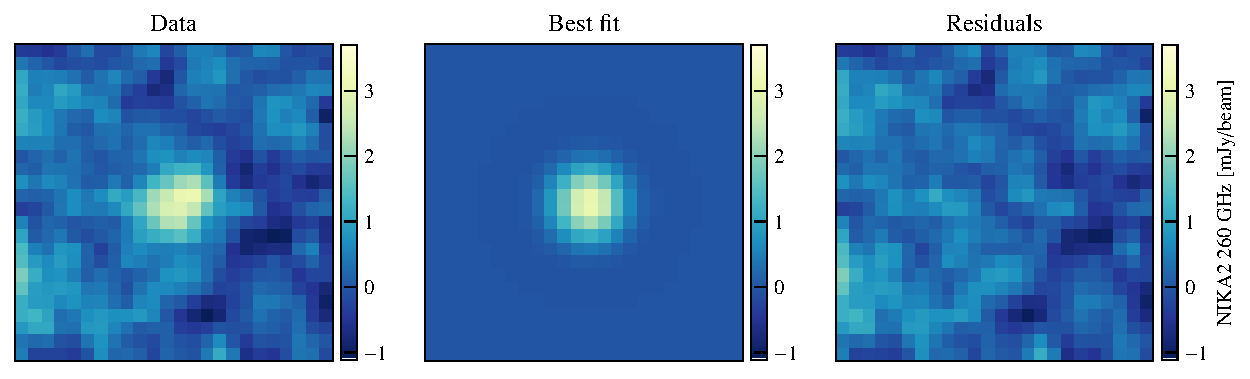
\includegraphics[width=.7\linewidth]{Figures/Chap_decor/4_1mm_fit.pdf}
    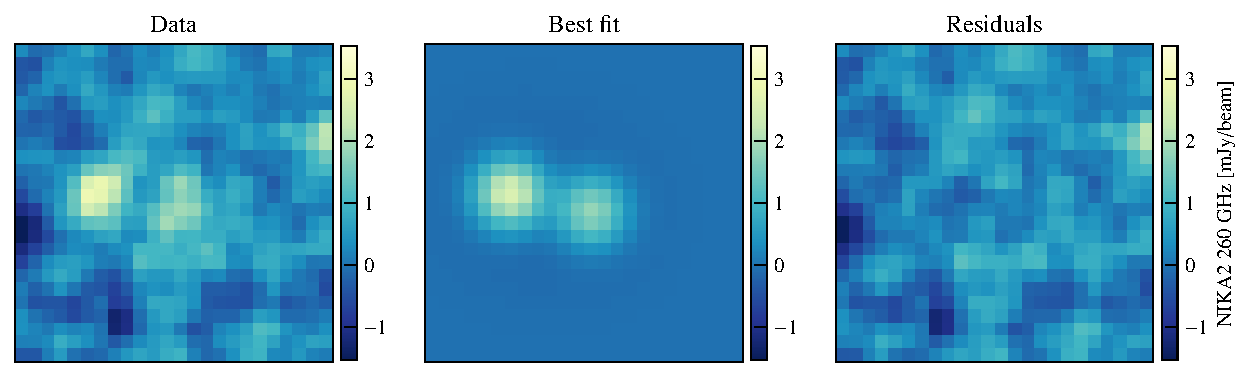
\includegraphics[width=.7\linewidth]{Figures/Chap_decor/2_1mm_fit.pdf}
    \caption{
        Résultats d'un ajustement de source à 260 GHz pour une source simple (\textit{haut}) et pour deux sources proches traitées comme double (\textit{bas}) dans le champ de l'amas \act.
        De gauche à droite, les cartes représentent les données NIKA2 à 260 GHz, le modèle correspondant au meilleur ajustement, et la différence entre les deux cartes.
    }
    \label{fig:pstools_1mm}
\end{figure*}

% ------------------------------------------------------------------------------------- %
\subsection{Ajustement du spectre de chaque source}

Le flux à 260 GHz de chaque source est ensuite combiné avec les trois flux SPIRE, permettant une couverture spectrale allant de 160 à 1200 GHz.
La SED de chaque source est ensuite ajustée sur ces quatre flux, en utilisant un modèle d'émission de corps noir modifié:
\begin{equation}
    F(\nu) = A_0 \left(\frac{\nu}{\nu_0}\right)^\beta B_\nu(T),
    \label{eq:pstools:sed}
\end{equation}
où $B_\nu(T)$ est le spectre d'un corps noir de température $T$, $A_0$ est l'amplitude de la SED à une fréquence de référence $\nu_0 = 500 \; \mathrm{GHz}$, $\beta$ est l'indice spectral de la poussière, et $T$ sa température effective, dégénérée avec le redshift de la source $z$ comme $T = T_\mathrm{dust} / (1+z)$.

L'ajustement de chaque SED est effectué en utilisant un échantillonnage Monte Carlo à chaînes de Markov (MCMC) et la librairie Python \texttt{emcee} \cite{foreman-mackey_emcee_2019}.
Le principe de fonctionnement du MCMC sera présenté au chapitre \ref{chap:panco}.
Nous considérons une fonction de vraisemblance gaussienne.
Lorsque les flux des sources ponctuelles dans les bandes de PACS ne sont pas disponibles, la couverture spectrale est relativement étroite, et ne permet pas de lever la dégénérescence entre les trois paramètres du modèle de corps noir modifié \cite{desert_submillimetre_2008,magnelli_herschel_2012,smith_isothermal_2013}.
Il n'est donc pas possible de laisser ces paramètres complètement libres, avec des \prior\ non-informatifs.
La normalisation de la SED, $A_0$, est donc ajustée linéairement sur les données et fixée pour chaque ajustement.
Enfin, un \prior\ sur l'indice spectral de chaque source est imposé par une distribution gaussienne $\beta \sim \mathcal{N}(2, 0.5)$, tel que suggéré par les mesures de SED de grands nombres de galaxies (voir par exemple \cite{magnelli_herschel_2012}).
Un \prior\ uniforme est utilisé pour la température effective de chaque source, $0 < T < 50 \; \mathrm{K}$.

À chaque étape du MCMC, une correction de couleur est appliquée aux flux mesurés afin de tenir compte de la différence entre le spectre de chaque source et celui de référence utilisé pour l'étalonnage des cartes.
Pour les flux SPIRE, la correction de couleur est interpolée \`a partir de mesures existantes\footnotemark ; pour le flux NIKA2, nous utilisons les corrections décrites dans \cite{perotto_calibration_2020}.
\footnotetext{\url{http://herschel.esac.esa.int/Docs/SPIRE/html/spire_om.html}, \S5.2.7}

À titre illustratif, la partie gauche de la figure \ref{fig:pstools_sed} montre le résultat de cet ajustement pour l'une des sources proches de l'amas \act.
Les flux utilisés pour contraindre le modèle sont représentés par les points bleus, et le modèle de SED résultant par la ligne bleue et les enveloppes d'erreur l'entourant.

\begin{figure}[tp]
    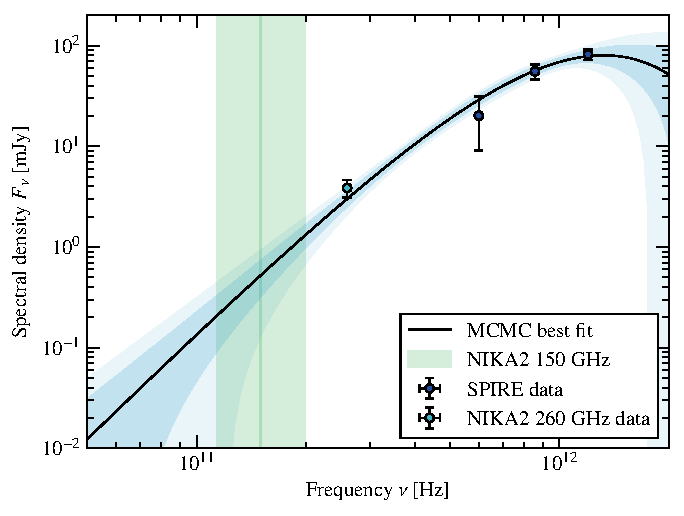
\includegraphics[width=0.48\linewidth]{Figures/Chap_decor/1_SED_no2mm.pdf}
    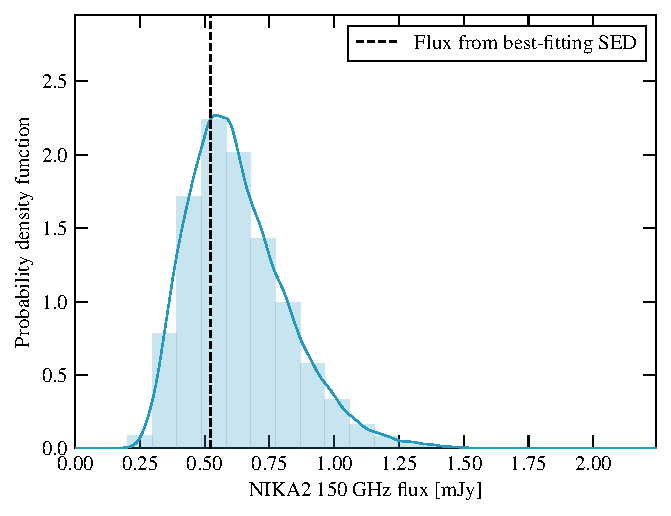
\includegraphics[width=0.48\linewidth]{Figures/Chap_decor/1_2mm_flux_dist.pdf}
    \caption{%
        \textbf{Gauche:} Résultat de l'ajustement de la SED de la source SMG1 dans le champ de l'amas \act, présenté au chapitre \ref{chap:actj0215}.
        Les points bleu foncé représentent des flux SPIRE.
        Les points bleu clair représentent le flux mesuré dans la carte NIKA2 à 260 GHz.
        La ligne bleue montre la SED ajustant le mieux les données, et les enveloppes l'entourant montrent les intervalles de confiance à $1\sigma$ et $2\sigma$.
        La région verte correspond à la bande passante à 150 GHz de NIKA2.
        \textbf{Droite:} Distribution de probabilité du flux de SMG1 dans la bande passante à 150 GHz de NIKA2.
        L'histogramme représente la distribution des flux calculés grâce au MCMC (voir texte).
        La courbe bleue montre la densité de probabilité obtenue en appliquant une estimation par noyaux à cette distribution.
        La ligne verticale noire montre le flux obtenu grâce à la SED ajustant le mieux les données.
        }
        \label{fig:pstools_sed}
\end{figure}

% ------------------------------------------------------------------------------------- %
\subsection{Inférence du flux à 150 GHz}

L'ajustement de SED produit pour chaque source un échantillonnage de la distribution de probabilité dans l'espace des paramètres $(\beta, T)$.
Chaque échantillon de cette distribution est alors utilisé pour calculer une SED grâce à l'équation (\ref{eq:pstools:sed}).
Chacune de ces SED est extrapolée pour calculer une valeur de flux à 150 GHz, et une correction de couleur est appliquée pour en déduire une valeur de flux attendue dans la bande passante de NIKA2.
La distribution de probabilité associée à ce flux est calculée à partir de ces mesures en utilisant une estimation par noyau (KDE pour \textit{Kernel Density Estimation}).
La combinaison de cette mesure avec l'ajustement des sources à 260 GHz nous donne accès, pour chaque source, à une connaissance précise de sa position et de la distribution de probabilité de l'amplitude de sa contamination de l'effet SZ à 150 GHz.
Le résultat de ce calcul est illustré dans la partie droite de la figure \ref{fig:pstools_sed}.

Le produit principal de \texttt{PSTools} est donc la distribution de probabilité du flux de chaque source dans la bande à 150 GHz de NIKA2.
Il existe plusieurs façons d'utiliser cette information pour traiter la contamination due à chaque source.
La plus simple consiste à soustraire un modèle de source à la carte NIKA2, avec un flux donné par le flux le plus probable issu de l'ajustement de SED, correspondant à la valeur maximisant la distribution de probabilités obtenue par \texttt{PSTools}.
Cette approche ne permet toutefois pas de tirer pleinement profit de l'information disponible, par exemple l'incertitude sur ce flux.
Nous verrons au chapitre suivant (section \ref{sec:panco_ps}) que les flux des sources peuvent être traités comme des paramètres de nuisance dans la modélisation de la carte de l'effet SZ d'un amas.
Cette approche permet de propager l'incertitude sur les flux des sources aux propriétés physiques de l'amas en utilisant la distribution de probabilités issue de \texttt{PSTools} comme \prior\ dans l'analyse.

% ===================================================================================== %
\section{Conclusions et perspectives}

Ce chapitre a présenté le traitement des données brutes de NIKA2 pour obtenir des cartes de l'effet SZ.
Nous avons vu en détail le principe de la décorrélation, c'est-à-dire l'extraction du signal astrophysique dans les observations NIKA2 dominées par différentes sources de bruit.
Le calcul de la matrice de covariance du bruit résiduel dans les cartes et du filtrage du signal a également été présenté.
Nous avons également présenté le logiciel \texttt{PSTools}, qui permet d'estimer l'amplitude de la contamination de l'effet SZ par des sources ponctuelles sub-millimétriques en combinant les observations NIKA2 et \textit{Herschel}.
Nous verrons dans le chapitre \ref{chap:panco} comment ces éléments sont inclus dans l'analyse des propriétés physique d'un amas pour tenir compte des effets systématiques qu'ils engendrent.

Comme nous l'avons discuté en \ref{sec:perf_decor}, la décorrélation est un processus imparfait, qui n'est pas en mesure de distinguer parfaitement le bruit du signal d'intérêt.
Sa performance peut se juger sur deux quantités mesurables: le spectre de puissance du bruit résiduel, et le filtrage du signal.
Comme nous le verrons au chapitre suivant, ces quantités servent à la fois de critères pour quantifier la performance de la décorrélation et d'outils pour tenir compte de son imperfection dans l'analyse des cartes NIKA2.
En pratique, le choix d'une méthode est basé sur un compromis entre filtrage et bruit résiduel.
En effet, les méthodes dites agressives, qui permettent d'atteindre un bruit résiduel très faiblement corrélé, sont en général caractérisées par un fort filtrage du signal d'intérêt.
À l'inverse, les méthodes préservant le mieux le signal sont en général moins performantes pour la soustraction du bruit corrélé.
Sur la base de ce compromis, la méthode \textit{common mode one block} est celle retenue pour l'analyse des observations du grand programme SZ de NIKA2.
Elle permet d'obtenir un filtrage relativement faible du signal aux échelles angulaires d'intérêt pour l'étude des amas de galaxies du grand programme SZ, au prix d'un bruit résiduel très corrélé.

Au sein du grand programme SZ de NIKA2, la décorrélation est réalisée à l'aide du \textit{pipeline} de la collaboration NIKA2, fruit d'un effort de la collaboration pour obtenir un outil permettant de passer des données en temps aux cartes du ciel.
J'ai développé un logiciel basé sur ce \textit{pipeline} pour réaliser ce traitement dans le cas des observations du grand programme SZ.
Ce logiciel permet d'interroger la base de données AMI du grand programme SZ, décrite en section \mypageref{sec:nk_ami}, pour obtenir la liste de \textit{scans} associés à un amas, réaliser la décorrélation de ces \textit{scans} et les coadditionner, puis de calculer la matrice de covariance du bruit résiduel et la fonction de transfert de la décorrélation.
Il a été mis a disposition de la collaboration, et est aujourd'hui systématiquement utilisé pour le traitement des données brutes des amas du grand programme SZ.

La décorrélation telle que présentée dans ce chapitre représente donc la procédure standard pour la décorrélation des données NIKA2 du grand programme SZ à l'heure de l'écriture de cette thèse.
L'amélioration de la procédure est toutefois un sujet très actif au sein de la collaboration NIKA2.
Parmi les axes d'amélioration en cours d'étude, de nouvelles méthodes de décorrélation sont en cours de développement et de test.
On notera en particulier le développement de méthodes novatrices, basées sur une décorrélation itérative sans masque.
Dans ces méthodes, à une itération $i$, plutôt que de masquer la région contenant du signal significatif dans la carte de l'itération $i-1$ dans le calcul du mode commun, la carte de l'itération $i-1$, supposée dominée par le signal d'intérêt, est soustraite aux données brutes.
L'intérêt est ici d'éviter de devoir estimer des modes communs sur trop peu d'échantillons.
Pour des sources étendues comme des amas de galaxies, masquer la région dans laquelle du signal est présent peut laisser peu de détecteurs pour l'estimation du mode commun, résultant en une mauvaise estimation du bruit.
Le processus itératif permet alors de converger vers une carte contenant le signal d'intérêt en ayant mieux retiré le bruit.
Ces méthodes ont mené à plusieurs tests au cours de cette thèse, dont les résultats sont encore très préliminaires.
Elles montrent une performance remarquable dans la soustraction du bruit corrélé, mais un filtrage important du signal astrophysique, qui est encore mal compris.
C'est pourquoi \textit{common mode one block} reste la méthode choisie pour les observations d'amas de galaxies avec NIKA2.

Un autre axe en cours de développement, intimement lié avec le développement de nouvelles méthodes, est le calcul de la fonction de transfert de la décorrélation.
La procédure présentée en \ref{sec:transfer_function} se base sur plusieurs hypothèses.
L'une de ces hypothèses a été discutée: nous avons supposé que le filtrage subi par le signal simulé au cours de notre analyse était identique à celui subi par le signal astrophysique d'intérêt.
En réalité, ces deux filtrages ne sont vraisemblablement pas exactement identiques.
La décorrélation de deux jeux de données, contenant le même bruit, mais dont l'un contient environ deux fois plus de signal que l'autre, peut être différente.
En particulier, les régions en périphérie du masque, dans lesquelles on trouve du signal significatif à $\lesssim 3\sigma$ dans l'analyse des données brutes de NIKA2, contiendront du signal plus significatif dans les données contenant le signal simulé.
Il est donc possible que l'estimateur de fonction de transfert présenté en \ref{sec:transfer_function} ne soit pas complètement juste.
Afin de quantifier cet effet, un travail est en cours pour créer des TOI entièrement synthétiques, contenant un bruit corrélé réaliste et du signal astrophysique pour chaque détecteur.
L'objectif est d'appliquer la procédure de décorrélation à ces TOI simulées pour évaluer la différence entre le filtrage réellement subi par un signal simulé, et l'estimateur de fonction de transfert présenté précédemment. \\
Une autre hypothèse implicite dans l'équation (\ref{eq:transfer_function}) est celle de l'isotropie du filtrage, c'est-à-dire de la symétrie circulaire du rapport entre les transformées de Fourier des cartes d'entrée et de sortie.
Cette hypothèse est justifiée par la stratégie de \textit{scan} du grand programme SZ de NIKA2, discutée en \ref{sec:map_coadd}, qui permet une couverture très isotrope de la région cartographiée en utilisant des \textit{scans} à différents angles.
Cependant, certaines directions peuvent rester privilégiées dans le filtrage, notamment les directions des \textit{scans}.
Une étude est donc en cours pour quantifier l'écart à la symétrie circulaire du filtrage subi par le signal d'intérêt lors de la décorrélation.
Les résultats en sont très prometteurs, montrant l'intérêt de l'utilisation de fonctions de transfert à deux dimensions pour les analyses du grand programme SZ \cite{munoz_echevarria_multi-probe_2021}.

La décorrélation reste donc un sujet d'étude actif, et les prochaines années permettront des avancées pour maximiser la qualité des cartes de l'effet SZ construites grâce aux observations NIKA2.


% ------------------------------------------- %
\chapter{Pipeline pour la mesure des propriétés thermodynamiques du milieu intra-amas}
\chaptermark{Pipeline pour la mesure de profils de pression}
\label{chap:panco}
\minitoc
L'objectif premier des observations d'amas de galaxies avec NIKA2 est de mesurer les propriétés thermodynamiques du milieu intra-amas.
En particulier, l'amplitude du signal tSZ mesuré en direction d'un amas permet la mesure de sa distribution de pression, qui peut ensuite être combinée à des observations X pour estimer la distribution de masse de l'amas, ainsi que d'autres propriétés thermodynamiques, comme décrit en section \mypageref{sec:lpsz_sci}.

Le logiciel \texttt{PANCO} (\textit{Pipeline for the Analysis of NIKA2 Cluster Observations}) développé par F. \myciteauthor{ruppin_cosmologie_2018} a pour objectif d'automatiser ce processus dans le contexte du grand programme SZ de NIKA2.
Au cours de ma thèse, après avoir utilisé ce logiciel, j'ai décidé d'en développer une version plus optimisée, basée sur l'utilisation de librairies Python dédiées au calcul numérique.
L'objectif de ce développement était double.
D'une part, il était nécessaire de fournir à la collaboration NIKA2 un code plus rapide, le temps d'exécution de \texttt{PANCO} étant trop grand pour permettre l'analyse d'échantillons d'amas.
D'autre part, il s'agissait d'une occasion de créer un outil standard pour le grand programme SZ de NIKA2, là où \texttt{PANCO} avait été développé pour l'analyse jointe de plusieurs cartes d'un même amas.

Ce nouveau logiciel, nommé \texttt{PANCO2}, a été rendu disponible pour la collaboration NIKA2, après avoir été testé sur des simulations.
Le temps d'exécution a été réduit d'un facteur dix à cent par rapport à \texttt{PANCO}.
Ce gain en performance a motivé le choix de \texttt{PANCO2} comme pipeline SZ officiel de la collaboration NIKA2.
Une généralisation du code est en cours, qui permettra d'utiliser \texttt{PANCO2} pour l'exploitation de cartes issues d'autres instruments, et qui sera livrée à la communauté comme un code public.
Ce chapitre décrit \texttt{PANCO2}, du principe de la mesure des propriétés thermodynamiques de l'ICM grâce à l'effet SZ à l'algorithme employé pour effectuer cette mesure.

\begin{figure*}[t]
    \centering
    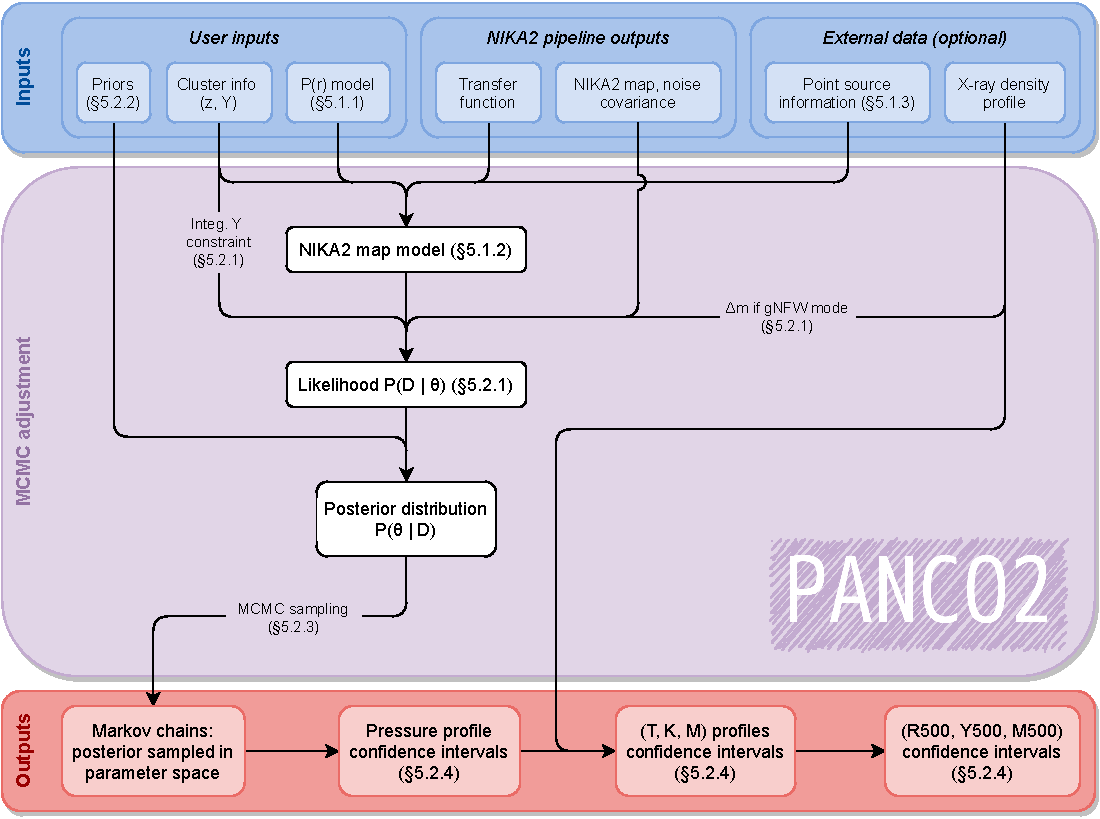
\includegraphics[width=.9\linewidth]{Figures/Chap_panco/panco2_workflow.pdf}
    \caption{
        Schéma représentant le principe de fonctionnement de \texttt{PANCO2}.
        Les données d'entrée sont les produits standards pour les observations NIKA2 d'amas de galaxies, produits par le pipeline d'analyse des données brutes présenté au chapitre \ref{chap:decorr}, ainsi que des données externes telles que les profils radiaux mesurés en X ou les informations sur les sources ponctuelles.
    }
    \label{fig:panco:schema}
\end{figure*}

Un schéma synoptique du fonctionnement de \texttt{PANCO2} est présenté en figure \ref{fig:panco:schema}.
Il répertorie les différentes données d'entrée (bleu) nécessaire à la mesure des propriétés thermodynamiques (rouge).
Les données principales sont les sorties du pipeline de la collaboration NIKA2, décrites au chapitre précédent.
Des informations sur la contamination par des sources ponctuelles, issues du logiciel \texttt{PSTools} détaillé en section \ref{sec:decor:pstools}, peuvent également être fournies -- elles seront discutées en \mypageref{sec:panco_ps}.
On note aussi la possibilité de donner en entrée un profil de densité mesuré en X, qui permettra la combinaison des données X et SZ pour une caractérisation détaillée des propriétés thermodynamiques du milieu intra-amas, discutée en \ref{sec:panco:thermo}.

% ==================================================================================== %
\section{Modélisation du signal SZ}

L'objectif principal de \texttt{PANCO2} est la mesure du profil de pression du milieu intra-amas à partir d'une carte de l'effet SZ.
Pour cela, une approche \textit{forward modelling} est employée.
Une modélisation de l'état physique du système, basée sur un nombre de paramètres, est établie, puis affectée des différents effets ayant donné naissance aux données observées.
Cela permet dans notre cas d'obtenir, à partir d'hypothèses physiques, un modèle de l'effet SZ mesuré par NIKA2, qui sera comparé aux données afin d'estimer les propriétés physiques de l'amas.
Cette section décrit les étapes successives nécessaires à l'obtention d'un tel modèle.

% ------------------------------------------------------------------------------------ %
\subsection{Profil de pression et effet Sunyaev-Zeldovich} \label{sec:panco:p_prof}

Comme décrit dans le chapitre~\ref{chap:amas}, l'effet Sunyaev-Zeldovich est une distorsion spectrale du fond diffus cosmologique due à la diffusion Compton inverse des photons sur les électrons du milieu intra-amas.
Dans le cadre de l'effet Sunyaev-Zeldovich thermique, dominant dans les observations NIKA2 d'amas de galaxies, l'énergie transférée par les électrons provient de leur grande agitation thermique.
L'amplitude de la distorsion observée aux coordonnées $\theta$ est alors appelée paramètre de Compton $y$, et est proportionnelle à la pression électronique $P_\e$ du milieu intra-amas intégrée le long de la ligne de visée (LdV) correspondante.
D'après l'équation (\ref{eq:sz_y}, page \pageref{eq:sz_y}), on a:
\begin{equation}
    \label{eq:panco:y_los}
    y(\theta) = \frac{\sigma_\textsc{t}}{m_\e c^2} \int_{\rm LdV(\theta)} P_\e(l) \; \d l .
\end{equation}

Par conséquent, la cartographie de l'effet SZ est une mesure directe de la distribution intégrée de pression du milieu intra-amas dans le plan céleste.
Bien que cette distribution ne soit pas mesurable le long de la ligne de visée, des hypothèses peuvent être faites sur la symétrie du milieu intra-amas.
Dans le cadre de l'hypothèse de symétrie sphérique, la distribution de pression ne dépend que de la distance au centre de l'amas, et est alors décrite par un profil radial de pression $P_\e(r)$.
Une carte de l'effet tSZ permet alors de contraindre ce profil de pression.
Par transformation d'Abel, l'équation (\ref{eq:panco:y_los}) devient:
\begin{equation}
    \label{eq:panco:y_abel}
    y(R) = 2\frac{\sigma_\textsc{t}}{m_\e c^2} \int_{R}^{+\infty} \frac{r}{\sqrt{r^2 - R^2}} \; P_\e(r) \; \d r .
\end{equation}

L'objectif principal de \texttt{PANCO2} est la mesure du profil de pression dans l'hypothèse de symétrie sphérique.
Dans \texttt{PANCO2}, je propose deux modélisations du milieu intra-amas, illustrées sur la figure \ref{fig:panco:gnfw_np}:
\begin{itemize}[leftmargin=*]
    \setlength\itemsep{5pt}
    \item Le modèle Navarro-Frenk-White généralisé (noté \guillemotleft gNFW \guillemotright), dans lequel le profil de pression est décrit par \cite{zhao_analytical_1996,nagai_effects_2007} :
    \begin{equation}
        \label{eq:panco:gnfw}
        P_\e(r) = P_0
        \left(\frac{r}{r_{\rm p}}\right)^{-c}
        \left[1 + \left(\frac{r}{r_{\rm p}}\right)^a \right]^\frac{c-b}{a} ,
    \end{equation}
    où $P_0$ représente la normalisation du profil, $b$ et $c$ les pentes externe et interne du profil de pression, et $r_{\rm p}$ et $a$ le rayon de transition entre les deux régimes et le caractère abrupt de cette transition;

\item Un modèle dit \guillemotleft non-paramétrique\footnotemark\guillemotright, dans lequel le profil de pression est décrit par des coquilles sphériques concentriques au sein desquelles la pression diminue avec le rayon en loi de puissance selon \cite{ruppin_non-parametric_2017,romero_multi-instrument_2018}:
    \begin{equation}
        \label{eq:panco:nonparam}
        P_\e(r) = P_i \left(\frac{r}{R_i}\right)^{-\alpha_i} .
    \end{equation}
\end{itemize}
\footnotetext{Il serait plus juste de parler de profil \guillemotleft binné \guillemotright, car le modèle est de fait paramétrique: ses paramètres sont les valeurs du profil de pression aux rayons spécifiés. Nous parlerons toutefois de modèle non-paramétrique par abus de langage, et par opposition au modèle gNFW dans lequel le nombre de paramètres est fixé par l'expression du modèle.}

Chacune des modélisations présente ses avantages et inconvénients.
Le profil gNFW est une fonction continue du rayon, aisément extrapolable et avec un nombre fixe de paramètres, le rendant plus directement comparable à la littérature dans laquelle il est le plus répandu.
Le profil non-paramétrique offre quant à lui une approche moins dépendante du modèle, et donc la possibilité de détecter des irrégularités dans le profil de pression, telles que des régions de surpression locales dues par exemple à des chocs.
Le plus grand avantage du profil non-paramétrique provient cependant des corrélations plus faibles entre ses paramètres, qui offre de meilleures performances dans l'ajustement, comme décrit dans la section \mypageref{sec:music_pressure}.

\begin{SCfigure*}[][t]
    \caption{
        Comparaison entre un profil de pression gNFW (bleu) et non-paramétrique (rouge).
        La valeur de la pression du profil non-paramétrique est divisée par deux à des fins de visibilité.
        Les lignes pointillées représentent l'extrapolation du profil non-paramétrique au-delà du premier et dernier point, en considérant une loi de puissance identique à celle entre le premier et deuxième point (à $r < R_{\rm min}$) et entre l'avant-dernier et le dernier point (à $r > R_{\rm max}$).
    }
    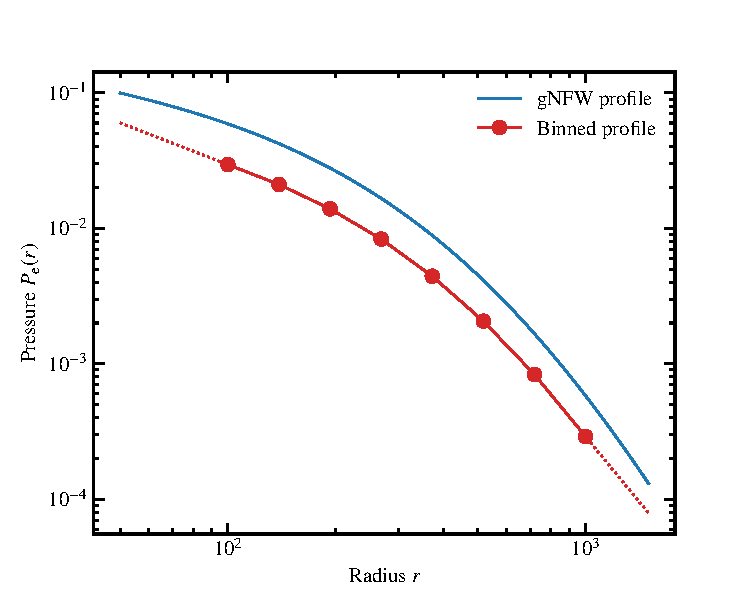
\includegraphics[width=.65\linewidth]{Figures/Chap_panco/gnfw_np.pdf}
    \label{fig:panco:gnfw_np}
\end{SCfigure*}

% ------------------------------------------------------------------------------------ %
\subsection{Modèle de carte de brillance de surface SZ}

Le profil de pression considéré est ensuite intégré le long de la ligne de visée afin d'obtenir une carte de paramètre de Compton $y$ dans la région de l'amas.
Dans le cas d'un modèle gNFW, l'intégrale de l'équation (\ref{eq:panco:y_los}) n'a pas de solution analytique, et une intégration numérique est utilisée, en considérant un grand nombre de pas espacés logarithmiquement le long de la ligne de visée afin de limiter les artefacts d'intégration.
Dans le cas d'un modèle non-paramétrique, l'intégrale de l'équation (\ref{eq:panco:y_abel}) est la somme des intégrales analytiques du profil de pression dans chacune des coquilles sphériques \cite{romero_multi-instrument_2018}.

La carte de paramètre de Compton obtenue doit ensuite être convertie en unités de brillance de surface afin d'être comparable aux données observées.
Le facteur de conversion dépend des bandes passantes effectives de NIKA2 (et donc des conditions atmosphériques au moment des observations), mais également du lobe de l'instrument.
Il dépend également de la forme du spectre de l'effet SZ, et donc de la température du milieu intra-amas du fait des corrections relativistes à l'effet SZ, comme décrit en section~\mypageref{sec:sz}.
En pratique, \texttt{PANCO2} traite ce facteur de conversion comme un paramètre de nuisance de l'analyse, ce qui permet de tenir compte de l'incertitude systématique liée à la variabilité de ce coefficient due aux conditions d'observations.

Les cartes de l'effet SZ réalisées par NIKA2 sont affectées par deux formes de filtrage.
Tout d'abord, l'image du ciel est convoluée par le lobe instrumental caractéristique du couplage entre NIKA2 et le télescope (décrit au chapitre~\ref{chap:nika2}).
Le modèle de carte de brillance de surface SZ est donc convolué par un filtre gaussien de largeur à mi-hauteur spécifiée par l'utilisateur.
Les cartes sont également affectées par le filtrage découlant de la procédure de soustraction du bruit des données en temps de NIKA2.
Ce filtrage est estimé par le calcul de la fonction de transfert présenté au chapitre \ref{chap:decorr}, et la carte de modèle est également convoluée par cette fonction de transfert.
La carte résultante est donc une carte étalonnée en unités de brillance de surface, affectée par le lissage des petites échelles angulaires caractéristique du couplage entre NIKA2 et le télescope, et par le filtrage des grandes échelles provenant de l'analyse des données brutes.
Elle peut donc être comparée à la carte de brillance de surface de l'effet SZ observée par NIKA2.

% ------------------------------------------------------------------------------------ %
\subsection{Contamination par des sources ponctuelles}\label{sec:panco_ps}

Le signal astrophysique mesuré par NIKA2 lors des observations d'amas de galaxies est la somme des contributions des différents objets présents le long de la ligne de visée.
Les contributeurs majeurs sont le milieu intra-amas par effet SZ, constituant l'observable d'intérêt pour les études présentées dans cette thèse ; ainsi que l'émission de sources ponctuelles.
Cette émission, par nature positive, peut compenser partiellement ou totalement le décrément SZ détecté dans les cartes NIKA2 à 150 GHz, et peut donc induire un biais négatif dans le profil de pression du milieu intra-amas reconstruit à partir des observations NIKA2.
La contamination résultante doit donc être prise en compte dans les mesures de propriétés du milieu intra-amas afin de ne pas souffrir de ce biais lors de l'utilisation des résultats du grand programme SZ en cosmologie.

Cette contamination peut être prise en compte en soustrayant des modèles de sources des données NIKA2.
Pour cela, il est nécessaire de connaitre la valeur du flux de chaque source, et une mauvaise estimation de ces flux peut induire une erreur dans les propriétés thermodynamiques mesurées.
\texttt{PANCO2} offre la possibilité de traiter cette contamination comme un paramètre de nuisance dans l'ajustement du profil de pression du milieu intra-amas.
Cette approche, présentée plus en détail dans le chapitre \ref{chap:actj0215}, permet de propager l'incertitude sur les flux des différentes sources ponctuelles à la mesure des propriétés thermodynamiques du milieu intra-amas.
Pour cela, des sources modélisées comme le lobe de NIKA2\footnote{Voir section~\ref{sec:nk_perf}.} peuvent être ajoutées au modèle de carte de brillance de surface présenté précédemment avant que celle-ci ne soit comparée aux données.
Les flux de ces sources sont alors considérés comme des paramètres supplémentaires du modèle.
La distribution de probabilité du flux de chaque source, obtenue avec \texttt{PSTools} (voir section \ref{sec:decor:pstools}), peut alors être utilisée comme \prior\ sur le paramètre, comme nous le verrons en section \ref{sec:panco:priors}.

% ------------------------------------------------------------------------------------ %
\subsection{Signal SZ intégré}

La couverture angulaire des observations SZ réalisées par NIKA2 est limitée par le filtrage des grandes échelles angulaires issu de la soustraction du bruit atmosphérique.
Ce filtrage se caractérise par une perte de signal en périphérie de l'amas, ce qui empêche l'établissement de contraintes fortes sur le profil de pression du milieu intra-amas dans ces régions.
Une information sur ce signal est contenue dans le signal SZ intégré de l'amas, mesuré dans les relevés à plus grand champ de vue desquels est issu le catalogue du grand programme SZ, à savoir les relevés \textit{Planck} \cite{planck_collaboration_planck_2016-2} et ACT \cite{hasselfield_atacama_2013}.
Ce signal est proportionnel à l'intégrale sphérique du profil de pression considéré jusqu'à un rayon donné $R$:
\begin{equation}
    Y_R = 4 \pi \frac{\sigma_\textsc{t}}{m_\e c^2} \int_0^R r^2 P_\e(r) \d r.
\end{equation}
Cette valeur peut donc être calculée à partir du modèle de profil de pression considéré, et comparée aux valeurs reportées dans les relevés SZ, imposant une contrainte effective sur le profil de pression dans les régions non contraintes par les observations NIKA2.
Les valeurs de $Y_{500}$ sont disponibles pour tous les amas du grand programme SZ de NIKA2, mesurées par \textit{Planck} ou ACT, et sont systématiquement utilisées afin d'améliorer la contrainte du profil de pression dans la périphérie de l'amas.

% ==================================================================================== %
\section{Ajustement par méthode Monte Carlo à Chaînes de Markov}
\label{sec:panco:fit}

Afin de déterminer le profil de pression du milieu intra-amas, le modèle de carte de brillance de surface décrit dans la section précédente est ajusté sur les données NIKA2 en utilisant un algorithme Monte Carlo à Chaînes de Markov (MCMC).
L'objectif est donc de trouver la distribution de probabilités des paramètres étant données les mesures effectuées par NIKA2.
Cette distribution, dite postérieure, est donnée par le théorème de Bayes :
\begin{equation}
    \label{eq:panco:bayes}
    P(\vartheta \,|\, D) = \frac{P(D \,|\, \vartheta) \, P(\vartheta)}{P(D)},
\end{equation}
où $\vartheta$ est le vecteur formé par les différents paramètres de l'analyse, résumés dans le tableau \ref{tab:panco:params}, et $D$ représente les données mesurées, qui dans le cas de \texttt{PANCO2}, sont la carte de brillance de surface mesurée par NIKA2 et le signal SZ intégré mesuré par ACT ou \textit{Planck}. \\
La distribution $P(D \,|\, \vartheta)$ est la fonction de vraisemblance comparant le modèle aux données, et $P(\vartheta)$ est notre connaissance \prior\ sur les valeurs des paramètres de l'analyse.
$P(D)$ est traitée comme une constante de normalisation permettant à l'équation (\ref{eq:panco:bayes}) d'être intégrable à 1.

% ------------------------------------------------------------------------------------ %
\subsection{Fonction de vraisemblance} \label{sec:panco:likelihood}

La fonction de vraisemblance, ou \textit{likelihood} en anglais, est la probabilité qu'un jeu de données $D$ soit issu d'un modèle $\vartheta$.
Dans \texttt{PANCO2}, j'ai choisi d'utiliser une fonction de vraisemblance Gaussienne multivariée dont chacun des pixels de la carte NIKA2 est une dimension :
\begin{equation}
    \label{eq:panco:like}
    \mathrm{log} \, P(D \, | \, \vartheta)
    = - \frac{1}{2}
        \big(D_\textsc{n} - \mathcal{M}_\textsc{n}(\vartheta)\big)^{\rm T}
        \Sigma_\textsc{n}^{-1}
        \big(D_\textsc{n} - \mathcal{M}_\textsc{n}(\vartheta)\big)
      - \frac{1}{2}
        \left(\frac{Y_R^{\rm meas.} - Y_R(\vartheta)}{\Delta Y_R^{\rm meas.}}\right)^2
      - \Delta_{\rm mass},
\end{equation}
où $D_\textsc{n}$ représente la carte NIKA2 à 150 GHz, $\mathcal{M}_\textsc{n}(\vartheta)$ le modèle de carte calculé à partir des paramètres $\vartheta$, et $\Sigma_\textsc{n}$ la matrice de covariance du bruit ;
$Y_R^{\rm meas.}$ et $\Delta Y_R^{\rm meas.}$ sont la mesure de signal SZ intégré dans un rayon $R$ et son incertitude, et $Y_R(\vartheta)$ le signal SZ intégré correspondant au modèle considéré (dans la suite, nous utiliserons $R = R_{500}$). \\
Cette fonction de vraisemblance permet donc de comparer un modèle aux observations réalisées avec NIKA2, en tenant également compte de la contrainte sur le paramètre de Compton intégré mesuré par \textit{Planck} ou ACT.
Dans le cadre d'un modèle gNFW, et si des données X sont fournies par l'utilisateur, le terme $\Delta_{\rm mass}$ est ajouté afin d'interdire les points pour lesquels le profil de masse décroit avec le rayon:
\begin{equation}
    \Delta_{\rm mass} =
        \begin{cases}
            \; 0 \;\text{si}\; \mathrm{d}M^{\rm HSE} / \mathrm{d}r \geqslant 0 \,\forall r, \\
            \; -\infty \;\text{sinon,}
        \end{cases}
\end{equation}
où $M^{\rm HSE}$ est calculé à partir de l'équation de l'équilibre hydrostatique (\ref{eq:mhse}). \\
Ce terme permet de restreindre l'espace des paramètres aux profils de pression ayant un sens physique, la masse contenue dans un rayon croissant ne pouvant pas diminuer.
Il n'est toutefois pas implémenté lors de l'ajustement d'un modèle non-paramétrique.
En effet, de telles analyses peuvent avoir pour objectif la mesure de surpressions locales, par exemple dues à des chocs.
Dans ces cas où l'équilibre hydrostatique n'est pas respecté, l'imposition d'une telle contrainte empêcherait la détection de telles particularités du profil de pression.
Cette contrainte n'est par conséquent imposée qu'au cours de l'ajustement de modèles gNFW, pour lesquels des fluctuations de pression ne sont de toute façon pas détectables, et qui bénéficient de la réduction de l'espace des paramètres au vu des fortes corrélations entre ces derniers.

% ------------------------------------------------------------------------------------ %
\subsection{Distribution \prior\ des paramètres}
\label{sec:panco:priors}

L'approche bayésienne utilisée dans \texttt{PANCO2} requiert la définition d'une distribution de probabilité \prior\ des paramètres $\vartheta$ qui sera combinée à la fonction de vraisemblance pour préciser la connaissance des paramètres.
Cette distribution est modélisée comme le produit de distributions définies individuellement pour chaque paramètre, soit en considérant chaque paramètre comme indépendant.
\texttt{PANCO2} propose plusieurs possibilités de distribution \prior\ pour chaque paramètre, résumées dans le tableau \ref{tab:panco:params}.
Notons en particulier que les paramètres correspondant au flux des sources ponctuelles peuvent prendre comme \prior\ la distribution de probabilité issue de \texttt{PSTools}, obtenue par ajustement du spectre des sources (voir section \ref{sec:decor:pstools}).

\afterpage{
\begin{table}[t]
    \setlength{\tabcolsep}{15pt}
    \footnotesize
    \centering
    \begin{tabular}{c l l}
        \toprule
        Paramètre & Description & Distribution \prior \\
        \midrule
        \midrule
        \multicolumn{3}{c}{\itshape Paramètres d'intérêt pour un modèle gNFW} \\
        \midrule
        $P_0, r_{\rm p}, a, b, c$ & Paramètres du profil de pression & -- Gaussiennes définies par l'utilisateur \\
          & & -- Uniformes avec limites choisies par l'utilisateur \\
        \midrule
        \multicolumn{3}{c}{\itshape Paramètres d'intérêt pour un modèle non-paramétrique} \\
        \midrule
        $P_i, \; i = 0 \dotsc n_{\rm bins}$ & Valeurs de pression & Uniformes entre 0 et 1 ${\rm keV \cdot cm^{-3}}$ \\
        \midrule
        \multicolumn{3}{c}{\itshape Paramètres de nuisance} \\
        \midrule
        $C_{\rm conv}$ & Conversion de $y$ en Jy/beam & Gaussienne définie par l'utilisateur \\[3pt]
        $Z$ & Niveau zéro de la carte & Gaussienne $\N(0,0.1 \; {\rm mJy/beam})$ \\[3pt]
        $F_i, \; i = 0 \dotsc n_{\rm PS}$ & Flux des sources ponctuelles & -- Distribution issue de \texttt{PSTools} (section \ref{sec:decor:pstools}) \\
        & & -- Uniformes avec limites définies par l'utilisateur \\
        \bottomrule
    \end{tabular}
    \caption{%
        Liste des paramètres utilisés par \texttt{PANCO2} pour modéliser les cartes SZ construites à partir d'observations NIKA2.
        La dernière colonne indique les distributions \prior\ utilisables pour chaque paramètre.
    }
    \label{tab:panco:params}
\end{table}
}

% ------------------------------------------------------------------------------------ %
\subsection{Échantillonnage de la distribution de probabilités}
\label{sec:mcmc_sampling}

L'ajustement du profil de pression est réalisé par échantillonnage Monte Carlo à Chaînes de Markov (MCMC) de la distribution postérieure définie par l'équation (\ref{eq:panco:bayes}).
L'avantage du MCMC par rapport à une maximisation de fonction de vraisemblance est l'obtention d'un ensemble de points de l'espace des paramètres distribués selon la postérieure de notre analyse, qui pourra ensuite être transposé dans l'espace des propriétés physiques du milieu intra-amas.

\subsubsection{Principe du MCMC} % --------------------------------------------------- %
Le principe de fonctionnement du MCMC repose sur une exploration de l'espace des paramètres par marche aléatoire, conditionnée par la valeur de la distribution de probabilités aux points visités.
Cette marche aléatoire peut être décrite par une série d'étapes successives :

\begin{enumerate}[leftmargin=*]
    \item La marche aléatoire commence en un point de l'espace des paramètres de coordonnées définies par un vecteur $\vartheta$.
        La valeur de la distribution de probabilités considérée est $P(\vartheta)$.
    \item Une position proche dans l'espace des paramètres, $\vartheta'$, est tirée au hasard d'après une fonction de proposition prédéfinie.
    \item Si $P(\vartheta') \geqslant P(\vartheta)$, alors $\vartheta'$ est automatiquement acceptée comme nouvelle position de l'échantillonneur ; sinon, elle est aléatoirement acceptée ou non avec une probabilité d'autant plus faible que $P(\vartheta') < P(\vartheta)$, nommée probabilité d'acceptance.
    \item La procédure est répétée autant de fois que nécessaire pour obtenir un nombre d'échantillons jugé suffisant.
\end{enumerate}

Ce processus peut être réalisé en parallèle par plusieurs marcheurs, créant chacun simultanément un ensemble de points nommé chaîne de Markov.
L'ensemble des positions $\vartheta$ acceptées par l'échantillonneur est alors distribué selon la fonction de distribution de probabilités considérée.

Un exemple commun de MCMC est donné par l'algorithme de Metropolis-Hastings \cite{metropolis_monte_1949,hastings_monte_1970}, où la fonction de proposition est une distribution Gaussienne de largeur constante et la probabilité d'acceptance est donnée par $p = P(\vartheta') < P(\vartheta)$.
Celui-ci est limité par la nécessité de définir au préalable une fonction de proposition immuable au cours de l'échantillonnage.
\texttt{PANCO2} utilise la librairie \texttt{emcee} \cite{foreman-mackey_emcee_2019}, proposant plusieurs implémentations en Python d'échantillonneurs adaptant leur fonction de proposition au cours de l'échantillonnage, introduits par \myciteauthor{goodman_ensemble_2010}.
En particulier, dans le cas de \texttt{PANCO2}, l'échantillonneur retenu est celui offrant les meilleures performances en termes d'échantillons indépendants générés par unité de temps, l'échantillonneur \texttt{DEMove} \cite{nelson_run_2013}.

\begin{figure}[t]
    \centering
    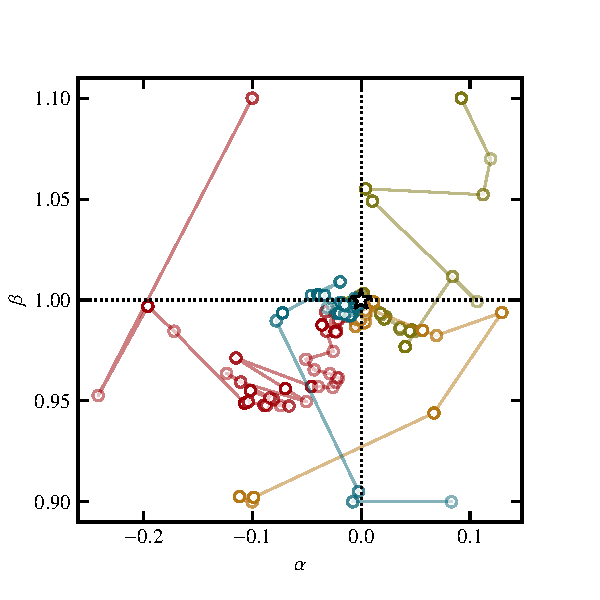
\includegraphics[width=.495\textwidth]{Figures/Chap_panco/mcmc_params.pdf}
    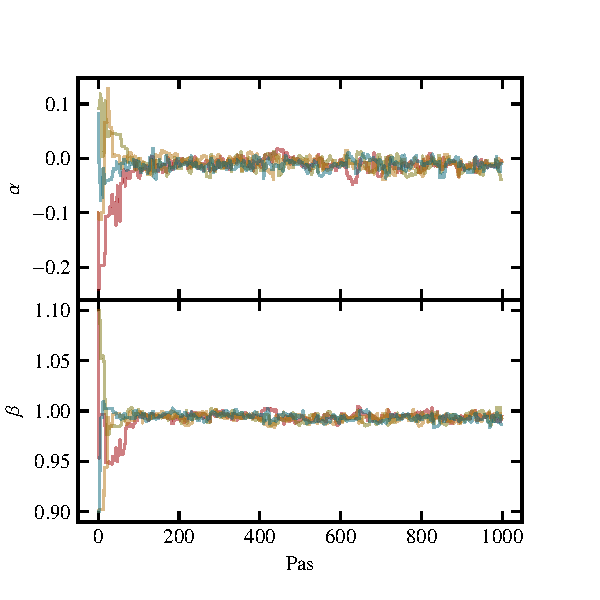
\includegraphics[width=.495\textwidth]{Figures/Chap_panco/mcmc_trace.pdf}
    \caption{
        Illustration du mouvement des chaînes d'un échantillonneur MCMC dans le cas d'une régression à deux paramètres $(\alpha, \beta)$, dans l'espace des paramètres (\textit{gauche}) et projeté pour chacun des paramètres individuellement (\textit{droite}).
        Chaque couleur représente une chaîne de Markov.
        L'étoile dans le panneau gauche représente le maximum de la distribution postérieure considérée.
    }
    \label{fig:panco:mcmc}
\end{figure}

\subsubsection{Convergence des chaînes et autocorrélation} % ------------------------- %
L'échantillonnage MCMC réalisé par \texttt{PANCO2} est automatiquement stoppé lorsque la convergence des chaînes a été atteinte, c'est-à-dire à partir de l'instant où l'ajout de nouveaux points aux chaînes de Markov n'apporterait pas d'information significative par rapport à ceux déjà générés.
La convergence est basée sur trois critères : l'adaptation des chaînes, leur mélange, et leur autocorrélation, décrite ci-après.

Le point de départ du MCMC dans l'espace des paramètres est arbitraire et ne se trouve pas nécessairement dans la région d'intérêt.
Par conséquent, il est nécessaire d'amputer chaque chaîne d'une longueur d'adaptation, correspondant au nombre de pas nécessaires à chaque marcheur pour rejoindre cette région d'intérêt.
Cette longueur, qualifiée de \textit{burn-in}, est systématiquement ignorée afin de ne considérer que les échantillons correspondant à des chaînes stationnaires et ne dépendant pas du point de départ arbitraire.
La figure \ref{fig:panco:mcmc} illustre cette adaptation : le panneau gauche montre le déplacement des marcheurs vers la région d'intérêt, symbolisée par l'étoile noire, et le panneau droit permet d'estimer une longueur de \textit{burn-in} d'environ une centaine de pas.

Le mélange des chaînes quantifie la similarité entre les distributions de points générés par chacune d'entre elles.
Des chaînes mélangées seront donc stationnaires et statistiquement similaires, comme illustré dans le panneau droit de la figure \ref{fig:panco:mcmc} dans le régime stationnaire.
Un critère permettant d'évaluer ce mélange est le critère de \myciteauthor{gelman_inference_1992}:
\begin{equation}
    \label{eq:panco:rhat}
    \hat{R} \equiv \sqrt{\frac{V}{W}} < 1.02
\end{equation}
où $W$ est la variance moyenne des échantillons d'une chaîne et $V$ la variance entre les différentes chaînes.

Les échantillons produits par la marche aléatoire décrite ci-dessus ne sont pas indépendants.
En effet, la position de chaque point dépend par construction de la position précédente.
On parle alors d'autocorrélation des chaînes.
La longueur moyenne séparant deux points pouvant être considérés indépendants peut être calculée d'après la série de positions acceptées formant la chaîne de Markov:
\begin{equation}
    \tau = 1 + 2 \sum_{i=1}^{n} \rho(\vartheta_0, \vartheta_i)
\end{equation}
où $n$ est la longueur de la chaîne considérée, et $\rho(\vartheta_0, \vartheta_i)$ est le coefficient de corrélation entre $\vartheta_0$ et $\vartheta_i$.

À intervalle régulier au cours de l'échantillonnage, \texttt{PANCO2} évalue ces trois critères, et accepte la convergence si :
\begin{itemize}[leftmargin=*]
    \setlength\itemsep{5pt}
    \item Toutes les chaînes ont parcouru une longueur supérieure à cinq fois la longueur de \textit{burn-in} définie par l'utilisateur ;
    \item Plus des deux tiers des chaînes passent le test de \citeauthor{gelman_inference_1992} (\ref{eq:panco:rhat}) ;
    \item Ces chaînes ont parcouru plus de cinquante fois leur longueur d'autocorrélation.
\end{itemize}
Les valeurs numériques utilisées dans ces tests sont des paramètres de l'analyse pouvant être modifiés par l'utilisateur.
Le choix particulier de deux tiers des chaînes et cinquante longueurs d'autocorrélation, utilisé par défaut, provient des tests sur simulations développés en section \ref{sec:panco:simus}.

% ------------------------------------------------------------------------------------- %
\subsection{Évaluation des propriétés thermodynamiques} \label{sec:panco:thermo}

Les chaînes de Markov produites par l'échantillonneur constituent un ensemble de points suivant la distribution de probabilité postérieure dans l'espace des paramètres du modèle.
On peut les écrire comme un vecteur $\mathbf{\vartheta}$, de dimension $n$ le nombre de points dans les chaînes, dont chaque composante $i \in [1 \dots n]$ est un vecteur dans l'espace des paramètres.
Cela permet de définir un vecteur de profils de pression $\mathbf{P}(r)$, dont chaque composante $i$ est le profil associé aux paramètres du point $\mathbf{\vartheta}_i$ des chaînes de Markov:
\begin{equation}
    \label{eq:panco:press_vec}
    \mathbf{P}(r) = P_\e(r, \mathbf{\vartheta_i}),
\end{equation}
où $P_\e(r)$ est le modèle de profil de pression choisi, gNFW ou non-paramétrique. \\
La distribution des composantes de $\mathbf{P}(r)$ permet donc d'étudier la distribution postérieure dans l'espace non plus des paramètres, mais des profils de pression.
On peut ainsi calculer l'incertitude sur le profil de pression comme la dispersion des composantes de $\mathbf{P}(r)$, ou encore comme les quantiles de cette distribution (les deux options sont implémentées dans \texttt{PANCO2}, et peuvent être choisis par l'utilisateur).

\subsubsection{Interpolations du modèle non-paramétrique} % --------------------------- %
\label{sec:panco:interp_np}
Dans le cas d'un modèle non-paramétrique, les paramètres du modèle sont les valeurs du profil de pression à différents rayons choisis par l'utilisateur.
La mesure de la pression à un rayon $r$ quelconque nécessite donc une interpolation (ou l'extrapolation) à partir de ces points.
\texttt{PANCO2} propose trois méthodes différentes, à choisir par l'utilisateur, pour interpoler le profil de pression pour la présentation des résultats finaux:
\begin{itemize}[leftmargin=*]
    \setlength\itemsep{0pt}
    \item L'interpolation en loi de puissance des points.
        C'est la méthode utilisée au cours de l'ajustement (voir équation \ref{eq:panco:nonparam}), et donc la plus naturelle.
        Cependant, comme nous l'avons décrit en \mypageref{sec:panco:p_prof}, le modèle non-paramétrique est une fonction dont la dérivée n'est pas continue.
        Le profil de masse hydrostatique étant justement proportionnel à cette dérivée, il peut présenter des discontinuités, rendant difficile l'estimation d'un profil de masse à partir de l'ajustement d'un tel modèle.
    \item Une interpolation en \textit{splines} du profil de pression.
        Si cette option est choisie, chacune des composantes du vecteur $\mathbf{P}(r)$ est interpolée par une fonction \textit{spline} dans le plan log-log, résultant en un profil de pression lisse et de dérivée continue.
        Cette méthode présente l'avantage de réaliser un lissage du profil, permettant l'estimation d'un profil de masse continu, tout en gardant l'aspect non-paramétrique du modèle utilisé pour l'ajustement.
        Cependant, son extrapolation est risquée, car les splines ne disposent d'aucune contrainte au delà de la région couverte par les rayons $R$ considérés dans le modèle.
    \item Une interpolation par un modèle gNFW.
        Dans ce cas, un modèle gNFW est ajusté sur chacune des composantes de $\mathbf{P}(r)$, et le modèle ajustant le mieux chaque profil est utilisé comme fonction d'interpolation.
        Les profils obtenus sont lisses et de dérivées continues, et leur extrapolation est rendue possible par le peu de variété dans les formes que peut prendre le modèle gNFW.
        En revanche, l'identification d'écarts à ce modèle n'est plus possible.
\end{itemize}
Quelle que soit la méthode choisie, elle permet de calculer le vecteur $\mathbf{P}(r)$ pour toute valeur de $r$ choisie.
La distribution des composantes du vecteur peut alors être étudiée pour évaluer l'incertitude sur le profil de pression.
La différence entre les profils de pression et de masse hydrostatique obtenus par l'utilisation de ces trois méthodes sera détaillée dans la section suivante (page \pageref{sec:panco:interp_np_results}), et illustrée en figure \ref{fig:panco:interp_np}.

\subsubsection{Profils thermodynamiques par combinaison avec les mesures X} % --------- %
\label{sec:panco:thermo_profiles_x}
Une fois que le vecteur $\mathbf{P}(r)$ a été construit, en calculant un profil de pression pour chaque jeu de paramètres issu des chaînes de Markov, celui-ci est combiné aux mesures X pour caractériser plus en détail les propriétés thermodynamiques du milieu intra-amas.
Pour cela, le vecteur $\mathbf{P}(r)$ est combiné avec le profil de densité X pour obtenir un vecteur de profils de température $\mathbf{T}$  d'après l'équation (\ref{eq:temperature}):
\begin{equation}
    k_\textsc{b} \mathbf{T}(r) = \mathbf{P}(r) \,\big/\, n_\e(r)
\end{equation}
et d'entropie $\mathbf{K}$ d'après l'équation (\ref{eq:entropy}):
\begin{equation}
    \mathbf{K}(r) = \mathbf{P}(r)\;n_\e^{-5/3}(r),
\end{equation}
et un vecteur de profils de masse à partir de l'équation de l'équilibre hydrostatique (\ref{eq:mhse}).
Comme pour le profil de pression, la dispersion des composantes de ces vecteurs donne l'incertitude sur les profils.
Comme nous l'avons vu en \mypageref{sec:lpsz_sci}, ces quantités permettent l'étude de la structure de l'amas et de son état dynamique, en exploitant la synergie entre observations SZ à haute résolution et X.
Une fois mesurées pour tout l'échantillon, elles pourront mener à des travaux sur le lien entre la physique de ces objets et les incertitude systématiques liées à leur exploitation cosmologique.

\subsubsection{Grandeurs caractéristiques intégrées} % -------------------------------- %
\label{sec:panco:integrated_qties}
Dans le cas du grand programme SZ de NIKA2, l'objectif est la mesure du profil de pression des amas, mais également de la relation d'échelle liant le paramètre de Compton $Y_{500}$ intégré dans un rayon $R_{500}$ à la masse $M_{500}$ contenue dans ce même rayon.
\texttt{PANCO2} permet de mesurer ces grandeurs en calculant le profil de masse hydrostatique à partir de l'équation de l'équilibre hydrostatique (\ref{eq:mhse}), puis en en déduisant le profil de contraste de densité $\delta_c(r)$ :
\begin{equation}
    \label{eq:panco:delta_c}
    \delta_c(r) = \frac{M_\mathrm{HSE}(<r)}{\rho_c(z) \times \frac{4}{3} \pi r^3}.
\end{equation}
où $\rho_c(z)$ est la densité critique de l'Univers au redshift $z$ de l'amas. \\
La procédure utilisée pour calculer les grandeurs intégrées est la suivante:
\begin{enumerate}[leftmargin=*]
    \item Le vecteur de profils de masse hydrostatique $\mathbf{M}_{\rm HSE}(r)$ est utilisé pour calculer un vecteur de profils de contraste de densité par l'équation (\ref{eq:panco:delta_c});
    \item Une valeur de $R_{500,i}$ est calculée pour chacune des composantes $i$ du vecteur de profils de contraste, en trouvant le rayon pour lequel il est égal à $500$;
    \item Une valeur de $Y_{500, i}$ est calculée pour chacune des composantes $i$ du vecteur $\mathbf{P}(r)$ par:
    \begin{equation}
        Y_{500, i} = 4\pi \frac{\sigma_\textsc{t}}{m_\e c^2}\int^{R_{500, i}} r^2 P_i(r) \, \d r,
    \end{equation}
    et une valeur de $M_{500, i}$ à partir des profils de masse hydrostatique:
    \begin{equation}
        M_{500, i} = M_i(R_{500, i}).
    \end{equation}
\end{enumerate}
Le résultat de cette procédure est donc un vecteur pour chacune des grandeurs caractéristiques $R_{500}$, $Y_{500}$ et $M_{500}$, dont chaque composante $i$ correspond à la grandeur estimée pour le point $\mathbf{\vartheta}_i$ des chaînes de Markov.
La distribution des composantes représente alors la distribution postérieure échantillonnée par le MCMC, dans l'espace des grandeurs intégrées, et peut être utilisée pour calculer les incertitudes entre les paramètres.
On note que les grandeurs intégrées sont par construction corrélées, comme déjà mentionné au chapitre \ref{chap:amas}.
Cette méthode d'estimation des grandeurs intégrées permet la mesure de cette corrélation en calculant la covariance des grandeurs intégrées mesurées pour chaque échantillon des chaînes de Markov.
La connaissance de cette covariance est cruciale à l'estimation des relations d'échelle, comme nous le verrons au chapitre \ref{chap:scaling}.
Les produits de \texttt{PANCO2} pourront donc être utilisés directement pour la mesure de la relation d'échelle $Y_{500}-M_{500}$ par la collaboration NIKA2.

% ===================================================================================== %
\section{Validation de \texttt{PANCO2} sur des amas simulés}
\label{sec:panco:simus}

Afin de s'assurer de la capacité de \texttt{PANCO2} à produire des mesures correctes de profil de pression, il est nécessaire de le tester sur des cartes d'amas dont le profil de pression est connu, et ainsi de comparer le profil évalué avec la vérité.
Pour cela, il est possible soit d'utiliser des observations réelles d'amas connus au profil de pression déjà caractérisé par d'autres instruments, soit de s'appuyer sur des simulations.
La première approche présente l'avantage de faire appel à des données réelles, mais est limitée par la connaissance imparfaite de l'amas observé.
L'analyse de simulations permet de connaitre parfaitement les propriétés physiques d'entrée, mais est limitée par la nécessité de créer des données réalistes et représentatives d'observations réelles.
La validation de \texttt{PANCO2} emploie la seconde approche, utilisant des amas synthétiques analytiques, puis un échantillon d'amas issu de la simulation hydrodynamique MUSIC \cite{sembolini_music_2013}.

% ------------------------------------------------------------------------------------- %
\subsection{Simulations d'amas simples} \label{sec:panco:demo}

La première analyse de validation de \texttt{PANCO2} est réalisée sur une carte d'amas synthétique similaire à l'un des amas du LPSZ.
Nous avons choisi l'amas \act, un des amas de faible masse et haut redshift de l'échantillon, dont les observations réelles seront présentées et analysées au chapitre \ref{chap:actj0215}.

Le milieu intra-amas de cette source synthétique est modélisé par un profil de pression gNFW, correspondant à celui mesuré par l'analyse effectuée sur les observations NIKA2 de l'amas \cite{keruzore_exploiting_2020}.
Des cartes de l'amas sont ensuite produites en intégrant ce profil de pression le long de la ligne de visée, et en filtrant la carte obtenue par le lobe de NIKA2 et par la fonction de transfert réelle de l'analyse.
Enfin, une réalisation de bruit blanc correspondant au niveau de bruit résiduel dans la carte de \act\ est ajoutée à la carte.

Les cartes obtenues sont ajustées avec \texttt{PANCO2} afin de tester sa validité sur des cas simples d'amas sphériques idéaux.
Cette analyse utilise un profil de pression non-paramétrique, dont les valeurs de rayons $R$ sont définies pour couvrir le signal attendu avec NIKA2, de son lobe à son champ de vue.
Cette distribution de rayons sera détaillée en \mypageref{sec:panco:binning}.
Dans cette section, nous décrivons les résultats pour cet amas synthétique, et présentons par la même occasion les figures produites par \texttt{PANCO2}.
Notons qu'une analyse similaire a été menée pour l'ajustement d'un modèle gNFW.
Les résultats sont très similaires pour les deux modèles (offrant une reconstruction non-biaisée du profil de pression), aussi ne présentons-nous ici que les résultats de l'ajustement d'un modèle non-paramétrique.

\subsubsection{Résultats de l'ajustement} % ------------------------------------------- %
Les résultats de l'ajustement permettent d'observer un accord entre le modèle ajusté par \texttt{PANCO2} et la vérité, utilisée pour générer les cartes.
La figure \ref{fig:panco2:actlike_dmr} montre la carte d'entrée et le meilleur ajustement de cette carte obtenu par \texttt{PANCO2}.
La différence entre ces deux cartes, représentant les résidus de l'ajustement, est compatible avec du bruit et ne permet pas d'identifier d'écart entre la vérité et l'ajustement.

\begin{figure*}[t]
    \centering
    \includegraphics[width=\linewidth]{Figures/Chap_panco/demo_plots/data_model_residuals.pdf}
    \caption{
        Carte simulée de \act\ (\textit{gauche}), carte de modèle ajustée par \texttt{PANCO2} (\textit{centre}), et différence entre les deux cartes (\textit{droite}).
        La région représentée est la même pour les trois cartes, et représente un carré de 5' de côté centré sur le centre simulé de l'amas.
        Les contours gris sont les niveaux de signal-sur-bruit, commençant à $3\sigma$ et espacés de $1\sigma$.
    }
    \label{fig:panco2:actlike_dmr}
\end{figure*}

\subsubsection{Chaînes de Markov et distribution postérieure des paramètres} % -------- %
La figure \ref{fig:panco2:actlike_chains} montre les chaînes de Markov, à savoir l'évolution des positions acceptées des marcheurs dans l'espace des paramètres avec le temps.
Chaque couleur correspond à un marcheur.
On voit que les chaînes ont atteint un état stationnaire, où elles n'évoluent plus à grande échelle et oscillent autour d'une valeur de paramètre correspondant à la valeur maximisant la distribution postérieure.
On voit également l'évolution à partir du point de départ, au cours des $\sim 200$ premiers pas.
La longueur de \textit{burn-in} retirée, représentée en gris, est de 1000 pas.

\begin{figure*}[t]
    \centering
    \includegraphics[width=0.9\textwidth]{Figures/Chap_panco/demo_plots/chains.png}
    \caption{
        Évolution des chaînes de Markov dans l'espace des paramètres avec le nombre de pas.
        Chaque couleur représente une chaîne distincte.
        La région grise correspond au \textit{burn-in} retiré pour l'analyse.
        Les lignes noires pointillées correspondent au vraies valeurs du coefficient de conversion et du niveau zéro de la carte.
    }
    \label{fig:panco2:actlike_chains}
\end{figure*}

La figure \ref{fig:panco2:actlike_corner} montre la distribution des positions des chaînes de Markov, c'est-à-dire la distribution postérieure, marginalisée sur chacun des paramètres (diagonale) et sur chaque combinaison de deux paramètres (éléments extra-diagonaux).
Cette figure représente donc la distribution postérieure échantillonnée dans l'espace des paramètres, qui sont les paramètres du profil de pression $P_i$, le coefficient de conversion et le niveau zéro de la carte.
Cette figure illustre donc à la fois les distributions de probabilité des paramètres et les corrélations entre ces paramètres.
On voit par exemple une forte corrélation entre le dernier point en pression $P_5$ et le niveau zéro de la carte: en effet, ajouter de la pression à très grand rayon, du fait de l'intégration le long de la ligne de visée, revient à ajouter un plateau quasi-constant à la carte.
La distribution de $\chi^2$ par degrés de liberté est également représentée, et est centrée en une valeur proche de 1, indiquant un bon ajustement des données par le modèle.

\begin{figure*}[p]
    \centering
    \includegraphics[width=0.95\textwidth]{Figures/Chap_panco/demo_plots/corner.pdf}
    \caption{
        Distribution postérieure dans l'espace des paramètres.
        Les éléments diagonaux représentent les distributions marginalisées sur chacun des paramètres, et les extra-diagonaux les distribution à deux dimensions pour chaque couple de paramètres.
        Les contours représentés sont les intervalles de confiance à $1\sigma$ et $2\sigma$.
        La ligne noire pointillée correspond à la vraie valeur du coefficient de conversion.
    }
    \label{fig:panco2:actlike_corner}
\end{figure*}

\subsubsection{Profils thermodynamiques} % -------------------------------------------- %
Le profil de pression issu de l'analyse est présenté en figure \ref{fig:panco2:actlike_press}.
On voit que le profil de pression mesuré par \texttt{PANCO2} (bleu) est en accord avec la vérité (noir) du lobe de NIKA2 jusqu'au delà de $R_{500}$, ce qui montre le succès de \texttt{PANCO2} pour cet ajustement.
L'interpolation utilisée pour estimer l'incertitude sur le profil de pression est l'interpolation gNFW, décrite en section \ref{sec:panco:interp_np}.
Les résultats des autres méthodes seront discutés par la suite (page \pageref{sec:panco:interp_np_results}).
Comme on peut le voir, le résultat est bien l'interpolation des points non-paramétriques par une fonction lisse: dans ce cas, un tel résultat était attendu, puisque le profil d'entrée est une fonction gNFW.
La matrice de corrélation entre les points du profil de pression est également représentée.
Celle-ci permet d'évaluer l'interdépendance des points du profil de pression, afin de déterminer si la distribution des rayons considérés pour le modèle est adaptée aux données.
Deux points trop proches seront en général fortement anti-corrélés, traduisant le fait que pour deux points très proches, augmenter l'un revient à diminuer l'autre.
La matrice de corrélation sera utilisée pour déterminer la distribution radiale optimale pour des amas synthétiques en section \ref{sec:panco:binning}.

\begin{figure*}[t]
    \centering
    \includegraphics[height=7.25cm, trim={0cm 0cm 1cm 0cm}, clip]{Figures/Chap_panco/demo_plots/pressure.pdf}
    \includegraphics[height=7.25cm, trim={1cm 0cm 0cm 0cm}, clip]{Figures/Chap_panco/demo_plots/pressure_correlations.pdf}
    \caption{
        \textbf{Gauche:} Profil de pression obtenu avec \texttt{PANCO2}.
        Les points bleus représentent le meilleur ajustement en non-paramétrique.
        L'enveloppe bleue représente l'incertitude sur ce profil obtenue par interpolation gNFW des résultats non-paramétriques.
        La courbe pointillée noire est le profil de pression utilisé pour générer la carte de l'amas.
        \textbf{Droite:} Matrice de corrélation entre les points du profil de pression, obtenue à partir des chaînes de Markov.
    }
    \label{fig:panco2:actlike_press}
\end{figure*}

Comme nous le verrons au chapitre suivant, \act\ a été observé par \textit{XMM-Newton}, et ces observations permettent d'extraire un profil de densité (représenté en figure \ref{fig:act:xmm}).
Puisque le profil de pression utilisé pour générer la carte NIKA2 est celui obtenu par ajustement des observations NIKA2 de l'amas réel, nous pouvons combiner ce profil de densité avec le profil de pression mesuré par \texttt{PANCO2} pour représenter les propriétés thermodynamiques de cet amas synthétique.
La procédure employée est décrite en \mypageref{sec:panco:thermo_profiles_x}.
Les profils obtenus par cette combinaison sont représentés en figure \ref{fig:panco2:actlike_thermo}.
On y trouve les profils de température et d'entropie du milieu intra-amas, ainsi que le profil de masse hydrostatique.
Les points bleus représentent les profils obtenus en non-paramétrique.
Comme pour le profil de pression, les enveloppes sont obtenues par interpolation gNFW, ce qui permet d'avoir un profil de masse continu.

\begin{figure*}[t]
    \centering
    \includegraphics[height=7.2cm, trim={0cm 0cm 1cm 0cm}, clip]{Figures/Chap_panco/demo_plots/temperature.pdf}
    \includegraphics[height=7.2cm, trim={0cm 0cm 1cm 0cm}, clip]{Figures/Chap_panco/demo_plots/entropy.pdf} \\
    \includegraphics[height=7.2cm]{Figures/Chap_panco/demo_plots/mass.pdf}
    \caption{
        Profils de température (\textit{haut gauche}), d'entropie (\textit{haut droit}), et de masse hydrostatique (\textit{bas}) obtenus par combinaison du profil de pression ajusté par \texttt{PANCO2} et du profil de densité mesuré en X pour \act.
        Les points bleus représentent la combinaison du meilleur ajustement du profil de pression en non-paramétrique avec le profil de densité mesuré en X.
        Les enveloppes bleues représentent l'incertitude sur ces profils obtenue par interpolation gNFW des résultats non-paramétriques.
    }
    \label{fig:panco2:actlike_thermo}
\end{figure*}

\subsubsection{Effet de la méthode d'interpolation} % --------------------------------- %
\label{sec:panco:interp_np_results}
Les résultats trois interpolations possibles pour le profil de pression, présentées en section \ref{sec:panco:interp_np}, sont présentées en figure \ref{fig:panco:interp_np}.
Les profils de masse correspondants sont également représentés.
Les résultats des trois méthodes sont similaires.
Dans les différences notables, on note une discontinuité dans le profil de masse à $r \simeq 300 \;\unit{kpc}$ pour l'interpolation non-paramétrique, due à la nature discontinue de ce modèle.
On observe également une incompatibilité entre les profils interpolés en \textit{splines} et les autres méthodes dans le centre de l'amas ($r \lesssim 100 \;\unit{kpc}$).
Au-delà de $400 \;\unit{kpc}$, les trois méthodes sont en excellent accord.
Le rayon caractéristique $R_{500}$ de cet amas étant de l'ordre de $800 \;\unit{kpc}$, cette similarité traduit un accord entre les trois méthodes pour l'estimation de la masse caractéristique $M_{500}$.
Le choix de la méthode d'interpolation dépend donc des objectifs scientifiques de l'analyse: la détection de surpressions locales nécessitera une interpolation en loi de puissance, alors que l'interpolation par un profil gNFW sera plus adaptée à l'étude d'un profil de masse continu dans le coeur de l'amas.

\begin{figure*}[t]
    \centering
    \includegraphics[width=.95\linewidth]{Figures/Chap_panco/demo_plots/interps.pdf}
    \caption{
        \textbf{Gauche:} Interpolations possible du profil de pression non-paramétrique (points blancs) pour un amas simulé: interpolation en loi de puissance (bleu), en \textit{splines} (vert), et en gNFW (rouge).
        La ligne continue montre le profil correspondant à l'interpolation du profil de pression ajustant le mieux les données
        \textbf{Droite:} Profils de masse hydrostatique obtenus par combinaison des profils de pression SZ et de densité X pour les trois méthodes d'interpolation.
        La ligne continue montre le profil correspondant au profil de masse obtenu à partir du profil de pression interpolé à partir du meilleur ajustement.
        Les régions colorées correspondent aux intervalles de confiance à $1\sigma$ sur les profils.
    }
    \label{fig:panco:interp_np}
\end{figure*}

\subsubsection{Grandeurs caractéristiques intégrées} % -------------------------------- %
Enfin, la combinaison des données X et SZ permet, à travers le profil de masse hydrostatique, de calculer les grandeurs intégrées caractéristiques de l'amas.
La procédure utilisée est décrite en \mypageref{sec:panco:integrated_qties}.
La distribution de probabilité obtenue par l'application de cette procédure à l'issue de l'ajustement de l'amas synthétique avec \texttt{PANCO2} est présentée en figure \ref{fig:panco2:actlike_integ}.
On y voit la forte corrélation entre les paramètres, de l'ordre de 80\% pour $R_{500}-Y_{500}$ et $M_{500}-Y_{500}$, et 95\% pour $R_{500}-M_{500}$ (qui sont calculés à partir du même profil de masse).
La distribution dans le plan $M_{500}-Y_{500}$ pour chaque amas du LPSZ est une donnée d'entrée pour l'ajustement de la relation d'échelle $Y_{500}-M_{500}$, discutée au chapitre \ref{chap:scaling}.

\begin{figure*}[t]
    \centering
    \includegraphics[width=.6\linewidth]{Figures/Chap_panco/demo_plots/integrated_values.pdf}
    \caption{
        Distributions des grandeurs caractéristiques intégrées $R_{500}$, $Y_{500}$, et $M_{500}$ obtenues par l'ajustement avec \texttt{PANCO2} de la carte simulée d'un amas synthétique.
        Les distributions présentées sont les distributions marginalisées à une dimension (éléments diagonaux) et à deux dimensions (éléments extra-diagonaux).
        Les contours présentés sont les intervalles de confiance à $1\sigma$ et $2\sigma$.
    }
    \label{fig:panco2:actlike_integ}
\end{figure*}

% ------------------------------------------------------------------------------------ %
\subsection{Optimisation de la distribution radiale} \label{sec:panco:binning}

Deux amas synthétiques considérés comme extrêmes pour le grand programme SZ ont été étudiés: un amas compact C1, de basse masse et haut redshift; et un amas étendu C2, de grande masse et bas redshift:
\begin{align}
    \label{eq:panco:synth_clusters}
    \nonumber \text{C1}: \; M_{500} = 3.5 \times 10^{14} \; M_\odot, \; z=0.9 ; \\
              \text{C2}: \; M_{500} = 9.5 \times 10^{14} \; M_\odot, \; z=0.5 .
\end{align}
Les propriétés thermodynamiques de ces amas ont été simulées en considérant une symétrie sphérique, et un profil de pression universel tel que mesuré par \myciteauthor{arnaud_universal_2010}.
Comme pour l'étude précédente, des cartes NIKA2 de ces amas sont simulées par intégration le long de la ligne de visée, conversion, filtrage par le lobe et par une fonction de transfert réaliste, puis ajout de bruit blanc réaliste.

Les cartes des amas C1 et C2 ont ensuite été utilisées afin d'optimiser le \textit{binning} du profil de pression, c'est-à-dire le choix des rayons $R_i$ considérés dans le modèle non-paramétrique de l'équation (\ref{eq:panco:nonparam}).
Ainsi, chacune de ces cartes a été ajustée pour plusieurs \textit{binning} différents, définis comme suit:
\begin{itemize}[leftmargin=*]
    \setlength\itemsep{0pt}
    \item Le premier rayon $R_0$ correspond à la demi-largeur à mi-hauteur (HWHM) du lobe de NIKA2, rayon en dessous duquel toute fluctuation de signal est lissée par la résolution de l'instrument;
    \item $n$ points sont ensuite ajoutés, espacés logarithmiquement entre $3 \times R_0$ et le rayon $R_{500}$ de l'amas ;
    \item Un dernier point à $2 \times R_{500}$ pour contraindre la pente externe du profil de pression.
\end{itemize}
L'ajustement est réalisé avec \texttt{PANCO2} sur les deux cartes d'amas simulées entre $n=2$ et $n=10$ dans le but de trouver la valeur de $n$ la plus adaptée aux amas du grand programme SZ.
Le choix du meilleur $n$ est basé sur deux critères.
Le profil de pression reconstruit par \texttt{PANCO2} doit être aussi proche que possible du profil réel utilisé en entrée de la simulation; et la corrélation entre deux points successifs du profil de pression $(P_i, P_{i+1})$ doit être minimale, symbolisant des mesures indépendantes du profil de pression à différents rayons.

Les résultats sont représentés sur la figure \ref{fig:panco:binning}.
Ils montrent qu'un amas étendu peut être modélisé avec un plus grand nombre de rayons qu'un amas compact, puisque l'extension de l'amas est plus grande par rapport au lobe de NIKA2 et dispose d'une meilleure couverture angulaire.
Pour l'amas compact C1, on voit qu'il est raisonnable de considérer jusqu'à $n=6$ points entre trois fois la demi-largeur à mi-hauteur du lobe de NIKA2 et le rayon caractéristique $R_{500}$ de l'amas avant que les résultats ne diffèrent grandement de la vérité.
D'autre part, on observe que la corrélation moyenne entre deux mesures de pressions successives augmente rapidement à partir de $n=4$.
Pour l'amas C2, les conclusions sont similaires: la justesse des résultats ne se dégrade que graduellement avec $n$, mais la corrélation entre deux points successifs augmente à partir de $n=5$.
Ces conclusions nous montrent que, quel que soit le critère choisi, les valeurs de $n$ optimales pour les amas les plus étendus et les plus compacts du grand programme SZ ne sont différentes que d'un point.
Par la suite, nous choisirons $n=5$, apparaissant comme la plus grande valeur utilisable avant que la corrélation des mesures de pression ne dépasse les 50\% pour les amas les plus compacts du programme.

\begin{SCfigure*}[][t]
    \caption{%
        Influence du nombre de rayons considérés dans le modèle non-paramétrique sur les résultats de \texttt{PANCO2}.
        $n$ est le nombre de points situés entre trois fois la demi-largeur à mi-hauteur du lobe de NIKA2 et le rayon caractéristique $R_{500}$ de l'amas (inclus).
        Les amas considérés sont des amas synthétiques ayant un profil de pression universel, considérant un amas compact (C1, bleu) et un amas étendu (C2, rouge) pour le grand programme SZ de NIKA2 (équation \ref{eq:panco:synth_clusters}).
        Le panneau du \textit{haut} représente l'évolution de la différence relative entre le résultat de \texttt{PANCO2} et la vérité intégré sur la plage de rayons considérés dans le modèle.
        Le panneau du \textit{bas} représente l'évolution de la corrélation moyenne entre deux points successifs du profil de pression.
    }
    \includegraphics[height=8cm]{Figures/Chap_panco/evol.pdf}
    \label{fig:panco:binning}
\end{SCfigure*}

% ------------------------------------------------------------------------------------ %
\subsection{La simulation MUSIC et l'échantillon jumeau du grand programme SZ}
\label{sec:panco:music}

La simulation MUSIC (\textit{Marenostrum-MultiDark SImulations of galaxy Clusters}, \cite{sembolini_music_2013}) est une simulation hydrodynamique d'amas de galaxies.
Elle est basée sur la technique de la resimulation par \textit{zoom-in} \cite{klypin_resolving_2001}, dont le principe de fonctionnement est rappelé ici.
Une simulation cosmologique à $N$-corps à relativement basse résolution  est réalisée pour simuler l'évolution de l'Univers, à partir de conditions initiales à haut redshift jusqu'à $z=0$.
Les résultats de cette simulation sont utilisés pour trouver les zones correspondant aux pics de densité de la toile cosmique formée, régions qui abritent les amas de galaxies dans l'Univers.
Ces régions sont ensuite resimulées, en repartant des mêmes conditions initiales, mais en ne considérant qu'un plus petit volume, correspondant à la région de l'amas seulement, ce qui diminue le temps nécessaire à la production des simulations.
Cette diminution de volume permet donc d'ajouter des ingrédients à la simulation, comme de la nouvelle physique, ainsi qu'un plus grand nombre de particules, augmentant ainsi la résolution finale de la simulation.

Dans le cas de MUSIC, les simulations d'entrée sont \textit{Marenostrum} \cite{gottlober_shape_2007} et \textit{MultiDark} \cite{prada_halo_2012}.
Un total d'environ 500 halos sont resimulés en incluant des phénomènes hydrodynamiques, de transfert radiatif et de formation stellaire.
Les amas resimulés offrent donc une physique bien plus riche que les halos d'origine, en plus d'une résolution un ordre de grandeur plus élevée.
Chaque amas est resimulé à partir de conditions initiales à un redshift $z=9$ jusqu'à $z=0$, et des \textit{snapshots} sont enregistrés à plusieurs redshifts intermédiaires afin de pouvoir étudier l'évolution des amas au cours du processus de formation des structures.

L'échantillon considéré pour la validation de \texttt{PANCO2} est un sous-ensemble de l'échantillon MUSIC sélectionné pour être similaire à l'échantillon du grand programme SZ de NIKA2.
Cet échantillon, créé par \myciteauthor{ruppin_impact_2019}, comporte 32 amas, couvrant une gamme de masse similaire à celle couverte par le grand programme SZ, à des redshifts de 0.54 et 0.82.
Les amas ont été sélectionnés afin d'avoir autant d'amas morphologiquement relaxés que d'amas perturbés.
Cet échantillon est particulièrement adapté à la validation de \texttt{PANCO2} : il est composé d'amas réalistes similaires à ceux du grand programme SZ de NIKA2.
Des observations NIKA2 simulées sont produites pour ces amas selon la procédure décrite dans \cite{ruppin_impact_2019}.
La pression -- connue -- du milieu intra-amas est intégrée le long d'une ligne de visée arbitraire afin d'obtenir une carte de paramètre de Compton, qui est ensuite convertie en unités de brillance de surface.
Celle-ci est ensuite convoluée par le lobe instrumental de NIKA2 et par une fonction de transfert fiducielle réaliste, et une réalisation de bruit corrélé est ajoutée suivant un spectre de puissance de bruit réaliste.
Les cartes résultantes sont donc des simulations réalistes d'observations avec NIKA2 des amas de l'échantillon.
Elles sont représentées sur la figure \ref{fig:panco:all_maps_music}.
On remarque une grande variété dans les morphologies d'amas, ainsi que dans le rapport signal sur bruit des observations.

\begin{figure*}[t]
    \centering
    \includegraphics[width=\linewidth]{Figures/Chap_panco/all_maps_music.pdf}
    \caption{Cartes simulées des 32 amas de l'échantillon utilisé pour la validation du code.
        Les échelles de couleurs sont arbitraires.
        Chaque carte est représentée dans un carré de 6.5' de coté, centré aux coordonnées du pic de densité du halo considéré.
        Les contours représentent les niveaux de signal sur bruit commençant à $3\sigma$ espacés de $1\sigma$.
        Les cartes sont lissées par un noyau gaussien de largeur à mi-hauteur 10''  pour des raisons visuelles.
    }
    \label{fig:panco:all_maps_music}
\end{figure*}

% ------------------------------------------------------------------------------------ %
\subsection{Ajustement du profil de pression} \label{sec:music_pressure}

Le profil de pression de chacun des amas de l'échantillon est estimé à l'aide de \texttt{PANCO2}.
Un modèle non-paramétrique est considéré : les profils de pression des amas MUSIC étant réalistes, toutes leurs caractéristiques ne peuvent pas être capturées par un modèle gNFW, rendant la comparaison d'un profil de pression ajusté par un tel modèle au vrai profil inappropriée.
Nous choisissons le même \textit{binning} que celui décrit dans la section \ref{sec:panco:binning} avec $n=5$ points entre la résolution de NIKA2 et $R_{500}$.
La fonction de transfert et la matrice de covariance du bruit utilisées pour générer les cartes simulées sont considérées dans l'analyse.

\begin{figure*}[p]
    \centering
    \includegraphics[height=6.5cm, trim={1.4cm 0.5cm 0.8cm 1.0cm}, clip]{Figures/Chap_panco/profiles_music/Bin1_cl00024_map.pdf} \hspace{10pt}
    \includegraphics[height=6.5cm, trim={0cm 0cm 1cm 1.0cm}, clip]{Figures/Chap_panco/profiles_music_2/00024.0.54.pdf}
    \includegraphics[height=6.5cm, trim={1.4cm 0.5cm 0.8cm 1.0cm}, clip]{Figures/Chap_panco/profiles_music/Bin1_cl00032_map.pdf} \hspace{10pt}
    \includegraphics[height=6.5cm, trim={0cm 0cm 1cm 1.0cm}, clip]{Figures/Chap_panco/profiles_music_2/00032.0.54.pdf}
    \includegraphics[height=6.5cm, trim={1.4cm 0.5cm 0.8cm 1.0cm}, clip]{Figures/Chap_panco/profiles_music/Bin2_cl00047_map.pdf} \hspace{10pt}
    \includegraphics[height=6.5cm, trim={0cm 0cm 1cm 1.0cm}, clip]{Figures/Chap_panco/profiles_music_2/00047.0.82.pdf}
    \caption{Illustration des cartes NIKA2 simulées (\textit{gauche}) et profils de pression mesurés (\textit{droite}) pour trois amas MUSIC: deux à $z=0.54$ (\textit{haut, milieu}) et un à $z=0.82$ (\textit{bas}).
        La légende des cartes est la même que pour la figure \ref{fig:panco:all_maps_music}.
        Les lignes pointillées noires représentent les profils de pression réels des amas tels qu'extraits de la simulation MUSIC.
        Les profils bleus sont ceux obtenus par ajustement avec \texttt{PANCO2}.
        Tous les profils sont centrés sur le pic de potentiel gravitationnel des amas tels que mesurés dans la simulation MUSIC.
    }
    \label{fig:panco:music_profs}
\end{figure*}

La convergence du MCMC est atteinte en environ une à deux heures par amas, représentant un gain d'un facteur $\sim 40$ par rapport à \texttt{PANCO}, qui réalisait l'ajustement des mêmes cartes en deux à trois jours par amas d'après \myciteauthor{ruppin_impact_2019}\footnotemark.
\footnotetext{Il est important de préciser que \texttt{PANCO} a été utilisé dans \cite{ruppin_impact_2019} pour ajuster simultanément des cartes simulées NIKA2 et \textit{Planck} des amas MUSIC, alors que l'analyse \texttt{PANCO2} décrite ici n'a considéré que les cartes NIKA2.}
Il est à noter qu'en considérant le bruit comme blanc -- c'est à dire en négligeant les éléments extra-diagonaux de la matrice de covariance du bruit -- \texttt{PANCO2} est capable de réaliser l'ajustement en cinq à quinze minutes par amas seulement, soit environ dix fois plus vite.
Ce constat motive grandement la poursuite du travail sur la soustraction du bruit corrélé dans les cartes NIKA2, afin d'obtenir des spectres de puissance de bruit résiduel les plus plats possibles et de pouvoir négliger les corrélations pixel-à-pixel du bruit dans les cartes.
Ce gain de temps permettrait de mener des études systématiques plus approfondies, comme l'évolution des résultats avec le \textit{binning} du profil de pression non-paramétrique sur l'ensemble des données du grand programme SZ de NIKA2.

Les résultats montrent un excellent accord entre les profils mesurés par \texttt{PANCO2} et ceux extraits de la simulation MUSIC.
Trois exemples sont présentés dans la figure \ref{fig:panco:music_profs}, illustrant la compatibilité entre le profil de pression réel et les résultats de \texttt{PANCO2} pour trois des amas de l'échantillon MUSIC.
On y voit un excellent accord dans les barres d'erreur entre les profils de pression ajustés par \texttt{PANCO2} et les données d'entrée sur toute la couverture radiale considérée dans l'ajustement, du lobe de NIKA2 à $2 \times R_{500}$, soit hors du champ de vue pour les amas considérés.
Cet accord permet de conclure que les résultats de \texttt{PANCO2} sont satisfaisants, même lorsque le logiciel est confronté à des données réalistes affectées des bruits et filtrages caractéristiques des observations d'amas avec NIKA2.

% ==================================================================================== %
\section{Conclusions}

L'observation des amas de galaxies du grand programme SZ de NIKA2 permet de mesurer la distribution de pression dans le milieu intra-amas individuellement pour chaque source.
L'approche choisie par la collaboration NIKA2 est le \textit{forward modelling}, permettant une prise en compte des différents phénomènes affectant les observations de l'effet Sunyaev-Zeldovich avec NIKA2.
Ce chapitre a présenté l'algorithme développé pour effectuer ces mesures en utilisant une procédure MCMC pour ajuster un modèle de profil de pression sur les données NIKA2.

Au début de ma thèse, cet algorithme était implémenté dans le logiciel \texttt{PANCO}, alors pipeline officiel du grand programme SZ de NIKA2.
Ce chapitre a présenté le développement de \texttt{PANCO2}, dont l'objectif était la livraison d'un logiciel offrant plus de possibilités d'analyse tout en étant plus rapide.
Le désir d'optimisation du temps d'exécution provenait du fait que \texttt{PANCO} ne permettait l'analyse d'un échantillon de plusieurs dizaines d'amas qu'au prix de plusieurs semaines de calcul, limitant l'exploitation des données du grand programme SZ de NIKA2.
L'analyse de cartes synthétiques d'un échantillon d'amas issus de la simulation hydrodynamique MUSIC a permis à la fois d'affirmer la capacité de \texttt{PANCO2} à estimer correctement le profil de pression d'amas de galaxies à partir de données NIKA2 réalistes, mais également de comparer ses performances à celles de \texttt{PANCO}.
Le temps d'exécution est diminué par un facteur d'environ quarante, rendant possible non seulement l'analyse d'échantillons d'amas en un temps raisonnable, mais également des études systématiques afin de tirer des informations plus fines sur les propriétés du milieu intra-amas à partir des observations NIKA2.
Ceci a mené au choix de \texttt{PANCO2} comme pipeline officiel du grand programme SZ de NIKA2, et à la préparation d'une mise à disposition de \texttt{PANCO2} pour la communauté scientifique.


% ------------------------------------------- %
\chapter{Mesure des propriétés thermodynamiques d'un amas distant de faible masse}
\chaptermark{Propriétés thermodynamiques de l'amas \act}
\label{chap:actj0215}
\minitoc
Les observations des amas de galaxies du grand programme SZ de NIKA2 ont commencé en 2017, avec l'observation de l'amas PSZ2-G144.83+25.11.
Cet amas a bénéficié d'un long temps d'observation dans le cadre de la phase de vérification scientifique de NIKA2.
Par conséquent, les cartes de cet amas offrent une détection hautement significative de l'effet SZ, jusqu'à $13\sigma$.
Cette grande qualité de données a permis une analyse certes profonde et détaillée des propriétés thermodynamiques du milieu intra-amas \cite{ruppin_first_2018}, mais qui n'est pas représentative des observations standard du LPSZ.

Ce chapitre présente la deuxième analyse individuelle d'un amas de galaxies dans le LPSZ.
Cette analyse présente plusieurs intérêts.
D'une part, elle constitue la première analyse de données de qualité standard pour le LPSZ.
D'autre part, elle se focalise sur \act, un amas distant et de faible masse, ayant pour conséquence un signal SZ faible et peu étendu.
Les cartes NIKA2 de cet amas sont de plus fortement contaminées par des sources ponctuelles, dont le flux compense une proportion non négligeable du signal SZ de l'amas (comme nous le verrons en page \pageref{sec:act:ps}).
Cet amas représente donc un banc d'essai pour les analyses des sources les plus complexes du grand programme SZ.
Cette analyse et ses résultats sont publiés dans \myfullcite{keruzore_exploiting_2020}.

% ==================================================================================== %
\section{Observations de ACT-CL J0215.4+0030}

% ------------------------------------------------------------------------------------ %
\subsection{Détection de l'amas par l'Atacama Cosmology Telescope}\label{subsec:act:act}

L'amas \act\ a été découvert par le premier relevé SZ de l'Atacama Cosmology Telescope (ACT), à un redshift de 0.865 \cite{menanteau_atacama_2013,hasselfield_atacama_2013}.
Il y a été détecté avec une signifiance de $5.5\sigma$.
Faute d'avoir une résolution angulaire suffisante pour résoudre des amas distants, le catalogue ACT reporte pour cet amas uniquement une mesure de signal SZ intégré, $Y_{500}$.
La masse de cet amas, estimée grâce à la relation d'échelle $Y_{500} - M_{500}$ publiée par \myciteauthor{arnaud_universal_2010}, est de $M_{500} = 3.8 \times 10^{14} \; M_\odot$.

% ------------------------------------------------------------------------------------ %
\subsection{Observations de l'amas avec NIKA2}\label{subsec:act:nk2}

Les observations NIKA2 de \act\ ont eu lieu lors de la quatorzième campagne d'observations de NIKA2.
Elles sont réparties sur cinq jours, entre le 17 et le 22 janvier 2018.
Toutes les observations de l'amas ont été effectuées entre 16h et 22h15 (UT).
La focalisation du télescope a été vérifiée au début de chaque série d'observations.
Le pointage du télescope et le lobe de NIKA2 ont quant à eux été vérifiés toutes les heures au cours des observations.
L'amas a été observé 8.6 heures au total, dans des conditions stables, avec une opacité moyenne à 225 GHz de $\tau_{225} = 0.175 \pm 0.05$.
Les distributions de l'opacité et de la transmission atmosphérique au cours des observations sont représentés sur la figure \ref{fig:act:scans}, montrant une grande proportion d'observations réalisées dans de mauvaises conditions (à des élévations inférieures à 30\textdegree, ou à des transmissions atmosphériques inférieures à 0.75).
Puisque les objectifs de rapport signal sur bruit du LPSZ demandaient 9 heures d'observations avec une opacité\footnote{correspondant à une transmission atmosphérique supérieure à 0.8, voir section \mypageref{sec:30m_geo}.} de $\tau_{225} = 0.1$, un bruit plus élevé que l'objectif est attendu dans les cartes NIKA2.

\begin{figure*}[t]
    \centering
    \includegraphics[width=\linewidth]{Figures/Chap_actj0215/scans.pdf}
    \caption{
        \textit{Gauche}: transmission atmosphérique $T$ en fonction de l'opacité $\tau$ et de l'élévation $el$.
        Chaque point blanc représente un scan de \act.
        \textit{Droite}: Distribution des opacités (\textit{haut}), élévations (\textit{centre}), et transmissions atmosphériques (\textit{bas}) pour les scans de \act.
    }
    \label{fig:act:scans}
\end{figure*}

Les observations ont été réalisées sous forme de plusieurs séries de quatre scans OTF, décrits en section \ref{sec:nk_otf_toi} de 8' $\times$ 4', chacun composé de 25 \textit{subscans}, avec des angles de 0, 45, 90 et 135 degrés par rapport à l'axe des ascensions droites.
Le centre de ces scans a été choisi aux coordonnées de l'amas reportées par le catalogue ACT \cite{menanteau_atacama_2013}, c'est-à-dire (RA, Dec)$_{\rm J2000}$ = (02h 15m 28.8s +00\textdegree 30' 33.0'')

Le pipeline de la collaboration NIKA2 décrit dans le chapitre \ref{chap:decorr} a été utilisé pour le traitement des données brutes de NIKA2.
La décorrélation du signal astrophysique et des différentes sources de bruit a été réalisée en utilisant la méthode \textit{Common mode one block}, décrite dans le chapitre \ref{chap:decorr}, ainsi que dans \myciteauthor{perotto_calibration_2020} sous le nom de \textit{most correlated pixels}.
Le masque utilisé pour le calcul du mode commun a été défini comme un disque de diamètre 2'  au centre de la carte.
Les itérations sur le masque basées sur des niveaux de signal sur bruit n'ont montré aucune amélioration des cartes, soustrayant au fur et à mesure des itérations plus de signal sans diminuer le niveau de bruit.
Par conséquent, la carte obtenue avec un masque circulaire a été retenue pour le reste de l'analyse.

La fonction de transfert, quantifiant le filtrage dû à la soustraction du bruit, ainsi que le spectre de puissance du bruit résiduel, sont produits automatiquement par le logiciel de réduction des données brutes utilisant le pipeline de la collaboration NIKA2 (cf. section \ref{sec:perf_decor}).
Ils sont tous deux présentés dans la figure \ref{fig:act:tf_noise}.
Il y apparaît que le signal est bien préservé aux petites échelles angulaires ($k > 0.5 \; {\rm arcmin}^{-1}$), et que le bruit résiduel est fortement corrélé.

\begin{figure}
    \centering
    \includegraphics[height=8cm, trim={0cm, 0cm, 0cm, 1cm}, clip]{Figures/Chap_actj0215/TF_noise.pdf}
    \caption{
        Spectre de puissance du bruit résiduel (\textit{haut}) et fonction de transfert (\textit{bas}) correspondant à l'analyse des observations de \act\ avec NIKA2
        La procédure d'obtention est décrite dans \ref{sec:perf_decor}.
        Le spectre de puissance montre un bruit résiduel corrélé à grande échelle, et la fonction de transfert montre le filtrage du signal aux grandes échelles angulaires.
    }
    \label{fig:act:tf_noise}
\end{figure}

Les cartes NIKA2 utilisées pour l'analyse sont présentées dans la figure \ref{fig:act:nkmaps}.
Dans la partie gauche, correspondant à la carte NIKA2 à 150 GHz, l'amas peut être identifié comme un décrément au centre de la carte, caractéristique de l'effet tSZ à des fréquences inférieures à 217 GHz.
Le maximum de ce décrément est détecté avec un rapport signal sur bruit de $8.5\sigma$.
On remarque dans cette carte un haut niveau de bruit résiduel, se manifestant par un gradient dans le sens sud ouest -- nord est.

La carte NIKA2 à 150 GHz montre également une indication de contamination par des sources ponctuelles.
Celles-ci émettent un flux positif qui peut compenser le décrément de l'effet SZ, et créer des trous\footnotemark\ dans la forme apparente du milieu intra-amas.
Une telle contamination est particulièrement inquiétante dans le cas de cet amas.
En effet, étant donné son faible signal (moins d'un mJy/beam au maximum) et sa petite extension spatiale (environ dix fois l'angle solide du lobe de NIKA2), la moindre contamination peut avoir de grandes conséquences sur les propriétés physiques reconstruites.

Dans la partie droite de la figure \ref{fig:act:nkmaps}, correspondant à la carte NIKA2 à 260 GHz, aucun signal SZ n'est détecté.
Le signal SZ positif attendu à ces fréquences ($\sim 0.2$ mJy/beam) est inférieur au niveau de bruit au centre de la carte par un facteur quatre.
En revanche, cette carte nous permet de confirmer la présence de sources ponctuelles proches du centre de l'amas, correspondant aux positions auxquelles des trous sont observés dans le signal SZ de l'amas.
Cela indique qu'une prise en compte soigneuse de la contamination par ces sources sera nécessaire à la mesure des propriétés thermodynamiques du milieu intra-amas.

\begin{figure}[t]
    \centering
    \includegraphics[width=\textwidth]{Figures/Chap_actj0215/nk_maps.pdf}
    \caption{
        Cartes NIKA2 du champ de l'amas à 150~GHz (\textit{gauche}) et 260~GHz (\textit{droite}).
        Chaque carte est montrée dans un champ carré de 4.5' $\times$4.5'  centré sur les coordonnées observées.
        Dans chacune des cartes, les contours noirs montrent les niveaux de signal sur bruit commençant à $3\sigma$ et espacés de $1\sigma$.
        Les cartes de gauche et droite sont lissées avec un noyau Gaussien de 10''  et 6''  respectivement pour des raisons visuelles.
        Pour chaque carte, la FWHM de sa résolution effective est illustrée par un disque blanc en bas de la carte.
    }
    \label{fig:act:nkmaps}
\end{figure}

% ------------------------------------------------------------------------------------ %
\subsection{Observations de l'amas avec \textit{XMM-Newton}}\label{subsec:act:xmm}

\act\ a été observé par \textit{XMM-Newton} pendant 37 ks.
Les données ont été récupérées depuis l'archive XMM, et les procédures standard (voir, par exemple, \cite{bartalucci_resolving_2017}) ont été suivies pour produire des fichiers étalonnés répertoriant les évènements enregistrés.
Les données ont été corrigées des effets de vignettage et du signal de fond.
Les sources ponctuelles ont été détectées et exclues.
Après ce nettoyage, le temps d'observation était de 35 ks sur les caméras MOS, et de 29 ks sur la caméra pn.

La carte lissée par ondelettes montrée sur la figure~\ref{fig:act:xmm} montre que le milieu intra-amas semble perturbé.
Les profils de densité et température électroniques corrigées de la PSF ont été produits à partir des données de \textit{XMM-Newton} en utilisant la déprojection décrite dans \cite{pratt_gas_2010}.
Au vu de la nature possiblement perturbée de l'amas, ces profils extraits aux pics X et SZ ont été comparés, mais aucune différence significative n'a été détectée.
Les profils 3D extraits au pic SZ sont montrés dans la partie droite de la figure \ref{fig:act:xmm}.
Le profil de température projeté, extrait directement à partir des spectres 2D, est aussi montré pour référence, mais seul le profil 3D est utilisé dans le reste de l'analyse.

\begin{figure}[t]
    \centering
    \includegraphics[height=7cm, trim={0cm, 0cm, 1cm, 1cm}, clip]{Figures/Chap_actj0215/xmm_map.pdf}
    \hfill
    \includegraphics[height=7cm, trim={0cm, 0cm, 1cm, 1cm}, clip]{Figures/Chap_actj0215/xmm_profs.pdf}
    \caption[XMM]{%
        \textbf{Gauche:} Carte d'évènements \textit{XMM-Newton} lissée par ondelettes.
        La région montrée est la même que dans la figure~\ref{fig:act:nkmaps}.
        Les iso-contours sont montrés en gris.
        \textbf{Droite:} Profils de densité (\textit{haut}) et température (\textit{bas}) électronique extraits à partir des observations XMM de l'amas.
        Les profils sont extraits aux coordonnées du pic SZ, comme décrit dans le texte (\ref{subsec:act:xmm}).
        Les barres d'erreur montrent les incertitudes à $1\sigma$.
        Pour le profil de température, la ligne rouge représente le profil projeté,tandis que les points blancs représentent le profil 3D reconstruit ; pour une explication détaillée de la différence entre les deux quantités, voir \cite{pratt_gas_2010}.
    }
    \label{fig:act:xmm}
\end{figure}

% ==================================================================================== %
\section{Contamination par des sources ponctuelles}\label{sec:act:ps}

Comme nous l'avons vu précédemment, une estimation précise de la contamination par des sources ponctuelles est nécessaire dans l'objectif de mesurer les propriétés du milieu intra-amas.
Cette étude est cruciale dans le cas de cet amas, étant donné son faible signal et sa faible extension spatiale.
Dans cette section, nous présentons la méthodologie utilisée pour estimer l'amplitude de cette contamination.

% ------------------------------------------------------------------------------------ %
\subsection{Identification des sources ponctuelles}

Dans le cas de \act, quatre sources sont identifiées avec un rapport signal sur bruit supérieur à 3 dans la carte NIKA2 à 260 GHz.
Leurs flux sont plus élevés à 260 GHz qu'à 150 GHz, favorisant l'hypothèse de sources sub-milimétriques (SMG) plutôt que radio.
Cette hypothèse est confirmée par l'identification de ces sources dans le catalogue HerS82 \cite{viero_herschel_2014}, construit grâce à l'instrument SPIRE à bord du satellite \textit{Herschel} qui a observé le ciel dans le domaine sub-millimétrique.
Ce catalogue nous permet également d'identifier une cinquième source dans le nord-est de l'amas.

La figure \ref{fig:act:composite} montre une carte composite multifréquence de la région de l'amas.
Les cercles verts sont centrés sur les positions des cinq SMG itentifiées dans le catalogue HerS82, et le diamètre de chaque cercle correspond à la FWHM du lobe instrumental de SPIRE à 250 $\mu$m, bande à laquelle la résolution angulaire de SPIRE est la meilleure.
Les régions rouges représentent les niveaux de rapport signal sur bruit dans la carte NIKA2 à 260 GHz lorsque celui-ci est supérieur à $3\sigma$.
NIKA2 et SPIRE sont en accord pour les positions des trois sources les plus proches de l'amas: de gauche à droite, SMG1, SMG2, et SMG4.
Dans le nord-est de l'amas, on trouve SMG3, qui est identifiée dans le catalogue HerS82 mais a un signal sur bruit inférieur à $3\sigma$ dans NIKA2 à 260 GHz.
Dans le sud de l'amas, deux sources semblent être résolues par NIKA2, mais seulement la plus faible des deux (S5) est identifiée dans le catalogue HerS82.
Il est par conséquent difficile d'estimer l'amplitude de leur contamination du signal SZ, puisqu'il n'existe pas de moyen de déterminer si le flux de S5 dans les bandes SPIRE provient d'une seule source ou de la somme des deux détectées dans NIKA2.
Ces sources étant jugées suffisamment éloignées de l'amas et de la zone dans laquelle le signal SZ est significatif, elles sont soustraites de la carte NIKA2 à 150 GHz dans la suite de l'analyse.

\begin{figure}[t]
    \centering
    \includegraphics[height=8.5cm, trim={10cm 5cm 8cm 5cm}, clip]{Figures/Chap_actj0215/composite.pdf}
    \caption{%
        Carte composite multifréquence de la région de l'amas.
        Les niveaux de bleu correspondent aux niveaux de signal sur bruit du décrément SZ dans la carte NIKA2 à 150 GHz, commençant à $3\sigma$ et espacés de $1\sigma$.
        De même, les niveaux de rouge correspondent au signal sur bruit des sources ponctuelles dans la carte NIKA2 à 260 GHz.
        Les cercles verts sont centrés sur les positions des sources dans le catalogue HerS82 \cite{viero_herschel_2014} et leur diamètre est la FWHM du lobe instrumental de SPIRE à 250 $\mu$m.
        La croix grise marque la position de S6, la source identifiée par NIKA2 qui n'a pas de contrepartie dans le catalogue HerS82.
        }
    \label{fig:act:composite}
\end{figure}

% ------------------------------------------------------------------------------------ %
\subsection{Estimation de la contamination}\label{subsec:act:sed}

Il est important de noter dans cette analyse l'absence d'information sur l'émission des sources à des fréquences supérieures à celles des bandes passantes de SPIRE ; par exemple, les études précédentes d'observations d'amas avec NIKA et NIKA2 tiraient parti de l'existence de données publiques de l'instrument PACS \cite{poglitsch_photodetector_2010}, qui ne sont pas disponibles ici.
Nous utilisons le logiciel \texttt{PSTools}, présenté en section \mypageref{sec:decor:pstools}, pour estimer l'amplitude de la contamination.
Le flux de chacune des sources est mesuré dans la carte NIKA2 à 260 GHz en ajustant un modèle de lobe instrumental de largeur fixe FWHM=12.5'', d'amplitude et de position libre, dans une portion carrée de largeur 1' autour de la position de la source dans le catalogue HerS82.
Les sources SMG1 et SMG2 étant proches, elles sont ajustées simultanément afin d'éviter une surestimation de leurs flux respectifs.
La SED de chaque source est ensuite ajustée par MCMC sur les points SPIRE et NIKA2 à 260 GHz, en considérant le modèle de corps noir modifié donné par l'équation (\ref{eq:pstools:sed}) et les \prior\ sur les paramètres présentés en \ref{sec:decor:pstools}.
Les échantillons dans l'espace des paramètres sont ensuite utilisés pour calculer une SED qui est extrapolée dans la bande passante de NIKA2 à 150 GHz, ce qui donne une estimation de la densité de probabilité de l'amplitude de la contamination.

La SED ajustée et la distribution de probabilité du flux à 150 GHz de chaque source sont présentés en figure \ref{fig:act:sed}.
On voit que l'ajustement de SED est correct pour toutes les sources, avec des modèles passant bien par les points.
On remarque également que la distribution de probabilité du flux de chaque source à 150 GHz n'est pas gaussienne, et apparaît asymétrique.
La capacité de \texttt{PSTools} à fournir ces distributions comme produit de sortie permettra de les utiliser comme \prior\ sur les flux des sources dans notre analyse, plutôt que de supposer une distribution gaussienne avec une valeur moyenne et une dispersion.

\begin{figure*}[p]
    \centering
    \includegraphics[height=0.23\textheight]{Figures/Chap_actj0215/PSPlots/1_SED_no2mm.pdf} \hspace{20pt}
    \includegraphics[height=0.23\textheight]{Figures/Chap_actj0215/PSPlots/1_2mm_flux_dist.pdf}
    \includegraphics[height=0.23\textheight]{Figures/Chap_actj0215/PSPlots/2_SED_no2mm.pdf} \hspace{20pt}
    \includegraphics[height=0.23\textheight]{Figures/Chap_actj0215/PSPlots/2_2mm_flux_dist.pdf}
    \includegraphics[height=0.23\textheight]{Figures/Chap_actj0215/PSPlots/3_SED_no2mm.pdf} \hspace{20pt}
    \includegraphics[height=0.23\textheight]{Figures/Chap_actj0215/PSPlots/3_2mm_flux_dist.pdf}
    \includegraphics[height=0.23\textheight]{Figures/Chap_actj0215/PSPlots/4_SED_no2mm.pdf} \hspace{20pt}
    \includegraphics[height=0.23\textheight]{Figures/Chap_actj0215/PSPlots/4_2mm_flux_dist.pdf}
    \caption{
        De haut en bas, résultats de \texttt{PSTools} pour les sources SMG1 à SMG4 dans le champ de l'amas \act.
        \textbf{Gauche:} ajustement de la SED sur les flux SPIRE (bleu foncé) et NIKA2 à 260 GHz (bleu clair).
        La région verte correspond à la bande passante de NIKA2 à 150 GHz.
        Les régions bleues correspondent aux intervalles de confiance à 1$\sigma$ et 2$\sigma$ sur l'ajustement de la SED.
        \textbf{Droite:} distribution de probabilité du flux à 150 GHz.
        L'histogramme représente les flux obtenus pour les chaînes de Markov, et la courbe bleue est la distribution de probabilité résultante.
    }
    \label{fig:act:sed}
\end{figure*}

% ------------------------------------------------------------------------------------ %
\subsection{Résultats}

La table \ref{tab:act:pscat} présente les flux et positions des six sources considérées dans cette analyse.
La dernière colonne présente le flux attendu dans la carte NIKA2 à 150 GHz de chaque source, obtenu par ajustement puis extrapolation de SED.
Il est important de noter que ces flux peuvent atteindre jusqu'à 0.74 mJy, alors que le pic d'émission SZ de l'amas est inférieur à 0.8 mJy/beam.
Cela accentue l'importance de la prise en compte de la contamination par les sources ponctuelles dans cette analyse.

L'une des sources (SMG2) présente également une émission radio.
Celle-ci est détectée dans le dernier catalogue FIRST \cite{helfand_last_2015} avec une densité de flux à 1.4 GHz de $2.22 \pm 0.10 \; \mathrm{mJy}$.
L'absence de couverture de la région de l'amas à d'autres fréquences radio rend impossible l'ajustement de la SED de l'émission radio de cette source.
Elle est donc modélisée par une loi de puissance $F(\nu) = F(\nu_0)\times(\nu/\nu_0)^\alpha$ avec un indice spectral $\alpha=-0.7 \pm 0.2$, qui est une bonne approximation de la SED de galaxies émettrices en radio \cite{condon_cosmological_1984}.
L'extrapolation de cette loi de puissance dans la bande passante à 150 GHz de NIKA2 donne une estimation de la densité de flux radio de cette source, $F_\mathrm{radio}(\mathrm{150\; GHz}) = 83 ^{+127}_{-50} \,\mathrm{\mu Jy}$.
Cette contribution est ajoutée à celle calculée par extrapolation de SED dans le domaine sub-millimétrique pour obtenir une estimation de la densité de flux totale de la source, bien que la contribution radio soit négligeable devant l'émission thermique de la poussière.

\begin{table*}[tp]
    \begin{center}
    \footnotesize
    \begin{tabular}{ccccccc}
        \toprule
        Source & Coordonnées J2000 & 1200 GHz & 860 GHz & 600 GHz & 260 GHz & 150 GHz \\
            &  & [mJy] & [mJy] & [mJy] & [mJy] & [mJy] \\
        \midrule
        SMG1 & $02^\mathrm{h}15^\mathrm{m}29.5^\mathrm{s}$ $+00^\circ30{}^\prime07.2{}^{\prime\prime}$ & 81.55 $\pm$ 9.77 & 55.39 $\pm$ 9.63 & 20.14 $\pm$ 11.08 & 3.85 $\pm$ 0.77 & 0.62 $\pm$ 0.19 \\
        SMG2 & $02^\mathrm{h}15^\mathrm{m}28.3^\mathrm{s}$ $+00^\circ30{}^\prime03.5{}^{\prime\prime}$ & 56.57 $\pm$ 9.83 & 46.87 $\pm$ 9.83 & 23.07 $\pm$ 10.57 & 2.64 $\pm$ 0.64 & 0.38 $\pm$ 0.14 $^{(a)}$\\
        SMG3 & $02^\mathrm{h}15^\mathrm{m}29.1^\mathrm{s}$ $+00^\circ31{}^\prime10.2{}^{\prime\prime}$ & 30.19 $\pm$ 9.68 & 29.45 $\pm$ 9.69 & 13.13 $\pm$ 10.6 & 1.42 $\pm$ 0.52 & 0.21 $\pm$ 0.09 \\
        SMG4 & $02^\mathrm{h}15^\mathrm{m}25.7^\mathrm{s}$ $+00^\circ30{}^\prime21.3{}^{\prime\prime}$ & 34.6 $\pm$ 9.86 & 25.84 $\pm$ 10.11 & 16.58 $\pm$ 10.43 & 4.42 $\pm$ 0.83 & 0.74 $\pm$ 0.25 \\
        S5 & $02^\mathrm{h}15^\mathrm{m}30.0^\mathrm{s}$ $+00^\circ29{}^\prime12.6{}^{\prime\prime}$ & -- & -- & -- & -- & 0.66 $\pm$ 0.19 $^{(b)}$\\
        S6 & $02^\mathrm{h}15^\mathrm{m}29.0^\mathrm{s}$ $+00^\circ29{}^\prime14.2{}^{\prime\prime}$ & -- & -- & -- & -- & 0.61 $\pm$ 0.19 $^{(b)}$\\
        \bottomrule\\
    \end{tabular}
    \normalsize
    \end{center}
    \vspace{-10pt}
    \caption{%
        Catalogue des positions et flux des six sources sub-millimétriques détectées dans un rayon de 2.5' autour du centre de \act.
        Les flux à 1200, 860 et 600 GHz proviennent du catalogue HerS82 \cite{viero_herschel_2014}.
        Les coordonnées et flux à 260 GHz sont obtenues par ajustement de modèles de lobe dans la carte NIKA2 à 260 GHz.
        Les flux à 150 GHz et leurs barres d'erreur sont les moyennes et écarts type des distributions de flux dans la bande passante de NIKA2.
        $^{(a)}$ Flux incluant l'émission radio.
        $^{(b)}$ Flux mesurés directement dans la carte NIKA2 à 150 GHz.
    }
    \label{tab:act:pscat}
\end{table*}

Les distributions de probabilité des flux à 150 GHz obtenues seront utilisées dans cette analyse afin de considérer la contamination par les sources ponctuelles comme des paramètres de nuisance lors de l'ajustement du profil de pression de \act.
Cette approche est préférée à une simple soustraction des sources dans le but de propager l'incertitude sur les flux des sources aux mesures des propriétés du milieu intra-amas, en traitant la contamination comme un effet systématique affectant l'analyse.
Cette procédure est décrite dans la section suivante.

% ==================================================================================== %
\section{Mesures des propriétés thermodynamiques du milieu intra-amas}

La mesure des propriétés thermodynamiques du milieu intra-amas de \act\ a été réalisée avant le développement de \texttt{PANCO2}, et a donc utilisé le logiciel \texttt{PANCO} \cite{ruppin_cosmologie_2018}.
L'algorithme en est décrit dans le chapitre \ref{chap:panco} (de même que les différences entre \texttt{PANCO} et \texttt{PANCO2}), aussi ne décrirons nous que brièvement la procédure employée.

% ------------------------------------------------------------------------------------ %
\subsection{Modélisation du milieu intra-amas}

Comme décrit dans les chapitres \ref{chap:amas} et \ref{chap:panco}, l'amplitude de l'effet SZ thermique, nommée paramètre de Compton $y$, est proportionnelle à la pression du milieu intra-amas intégrée le long de la ligne de visée (équation \ref{eq:sz_y} page \pageref{eq:sz_y}).
Nous modélisons le milieu intra-amas comme une structure de gaz à symétrie sphérique, dont la distribution radiale de pression est décrite par un modèle de profil Navarro-Frenk-White généralisé (gNFW, \cite{nagai_effects_2007}):

\begin{equation}
    P_\e(r) = P_0 \left(\frac{r}{r_p}\right)^{-c}
        \left[1 + \left(\frac{r}{r_p}\right)^{a}\right]^{(c-b)/a},
\end{equation}
où $P_0$ est la normalisation du profil de pression, $b$ et $c$ sont les pentes du profil dans les régions externes et internes de l'amas respectivement, et $r_p$ et $a$ quantifient respectivement le rayon et la vitesse de la transition entre les deux régimes.

% ------------------------------------------------------------------------------------ %
\subsection{Analyse MCMC}

\texttt{PANCO} utilise une procédure Monte Carlo à Chaînes de Markov (MCMC) pour ajuster le profil de pression du milieu intra-amas sur la carte NIKA2 à 150 GHz.
À chaque pas du MCMC, un profil de pression gNFW est intégré le long de la ligne de visée pour obtenir un profil de paramètre de Compton $y$.
Ce profil est ensuite projeté sur une grille pixelisée de la même façon que la carte NIKA2 pour obtenir une carte de paramètre de Compton.
Cette carte est convoluée par le lobe de NIKA2, modélisé par une Gaussienne à deux dimensions de largeur à mi-hauteur $\mathrm{FWHM=18.5}$'', en accord avec l'étalonnage des cartes NIKA2 \cite{perotto_calibration_2020}.
La carte est centrée aux coordonnées du pic de brillance de surface SZ dans la carte NIKA2 à 150 GHz.
%
La carte est ensuite convertie en unités de brillance de surface à l'aide d'un coefficient de conversion $C_\mathrm{conv}$.
Ce coefficient dépend de la forme de la distorsion spectrale de l'effet SZ, mais également des bandes passantes de NIKA2, de son lobe instrumental, et de l'opacité atmosphérique, qui varie au cours des observations.
Par conséquent, le coefficient est traité comme un paramètre de nuisance et ajusté avec les paramètres du profil de pression, avec un \prior\ Gaussien d'écart type 10\% dans le but de tenir compte de l'incertitude sur l'étalonnage absolue des cartes NIKA2.

La contamination par les sources ponctuelles est ajustée simultanément avec le profil de pression du milieu intra-amas, plutôt que simplement soustraite en utilisant les flux des sources obtenus par extrapolation de SED.
Chaque source est modélisée par un modèle de lobe de NIKA2 d'amplitude libre ajouté au modèle de carte de l'effet SZ.
Le flux de chaque source est traité comme un paramètre de nuisance, avec un \prior\ donné par la distribution de probabilité calculée dans la section \ref{sec:act:ps}.
Cette procédure présente l'avantage de tenir compte de l'incertitude sur les densités de flux extrapolées dans l'ajustement du profil de pression.
Les sources S5 et S6 sont quant à elles jugées assez éloignées de l'amas pour être directement soustraites des données.
Le modèle de carte de brillance de surface obtenu, modélisant simultanément l'effet SZ et la contamination par les sources ponctuelles, est convolué par la fonction de transfert présentée dans la figure \ref{fig:act:tf_noise} afin de tenir compte du filtrage créé par le pipeline NIKA2.

La couverture angulaire de NIKA2 et le filtrage des grandes échelles par la soustraction du bruit corrélé limite la possibilité de contraindre le profil de pression dans la périphérie de l'amas.
De telles contraintes peuvent toutefois être établies en utilisant la valeur du signal SZ intégré dans un rayon de $R_{500}$ :
\begin{equation}
    \mathcal{D}_\mathrm{A}^2 \; Y_{500} = 4\pi \frac{\sigma_\textsc{t}}{m_\e c^2}\int_0^{R_{500}} r^2 P_\e(r) \, \d r,
\end{equation}
où $\mathcal{D}_\mathrm{A}$ est la distance diamètre angulaire jusqu'à l'amas.
Le paramètre de Compton intégré de l'amas a été mesuré dans le relevé ACT, avec une valeur publiée de \cite{hasselfield_atacama_2013}
\begin{equation}
    \mathcal{D}_\mathrm{A}^2 \, Y_{500}^\mathrm{ACT} = (4.07 \pm 1.13) \times 10^{-5} \;\mathrm{Mpc}^2
\end{equation}
Cette contrainte est incluse dans la fonction de vraisemblance de l'ajustement du profil de pression : à chaque pas du MCMC, la valeur de $Y_{500}$ est calculée et comparée à cette mesure, imposant une contrainte effective sur le signal SZ à grande échelle.

En résumé, à chaque pas du MCMC, un modèle de carte est calculé à partir d'un jeu de paramètres $\vartheta$ comprenant:
\begin{itemize}
    \setlength\itemsep{0pt}
    \item $P_0$, $r_p$, $a$, $b$, et $c$ : les paramètres décrivant le profil de pression gNFW du milieu intra-amas ;
    \item $F_{150}^i$, $i = 1 \dots 4$ : les densités de flux des sources ponctuelles proches de l'amas ;
    \item $C_\mathrm{conv},\,Z$ : le coefficient de conversion de $y$ vers Jy/beam et le niveau zéro de la carte.
\end{itemize}
La probabilité qu'un jeu de paramètres décrive nos données est obtenue en combinant la distribution \prior\ sur les paramètres et la fonction de vraisemblance $\mathcal{L}$ comparant le modèle de carte $\mathcal{M}$ aux données $\mathcal{D}$ :
\begin{equation}
    \mathrm{log}\,\mathcal{L}(\vartheta) =
        -\frac{1}{2}
        \big(\mathcal{M}(\vartheta) - \mathcal{D} \big)^T
        \Sigma^{-1}
        \big(\mathcal{M}(\vartheta) - \mathcal{D} \big)
        - \frac{1}{2}
        \left(\frac{Y_{500}^\mathrm{ACT} - Y_{500}(\vartheta)}{\Delta Y_{500}^\mathrm{ACT}}\right)^2,
    \label{eq:likelihood}
\end{equation}
où $\Sigma$ est la matrice de covariance du bruit, évaluée à partir de $10^5$ réalisations aléatoire de bruit corrélé générées à partir du spectre de puissance présenté sur la figure \ref{fig:act:tf_noise}.
Cette distribution de probabilité est échantillonnée à l'aide de la librairie Python \texttt{emcee} \cite{foreman-mackey_emcee_2019}.
La convergence des chaînes est contrôlée à intervalle régulier à l'aide du test de Gelman-Rubin \cite{gelman_inference_1992}.
Une fois la convergence atteinte, une longueur de \textit{burn-in} est enlevée au début de chaque chaîne.

% ------------------------------------------------------------------------------------ %
\subsection{Auto-consistance des estimations de flux des sources ponctuelles}
\label{sec:act:ps_flat_prior}

Les paramètres évalués lors de la reconstruction du milieu intra-amas incluent les flux des sources ponctuelles proches de l'amas.
La comparaison des flux retrouvés par l'analyse MCMC avec ceux obtenus par extrapolation de SED révèle un accord des mesures.
Cependant, puisque les résultats utilisant l'extrapolation de SED sont utilisés comme \prior\ dans l'analyse jointe du milieu intra-amas et des sources, les résultats ne sont pas indépendants.
À fin de comparaison, l'analyse MCMC décrite dans la section précédente a donc été répétée sans utiliser d'\prior\ sur les flux des sources.
Les résultats de cette comparaison sont représentés sur la figure \ref{fig:act:pscomp}.
Pour chaque source, les mesures de flux sont compatibles à $1\sigma$.
Ce résultat renforce la confiance dans l'estimation des flux des sources, et donc dans l'estimation du signal SZ dans les régions contaminées.
De plus, bien que cette compatibilité montre que l'extrapolation de SED n'apporte que peu d'information utile au MCMC, l'utilisation d'\prior\ sur les flux des sources réduit grandement le volume de l'espace des paramètres accessible par le MCMC, réduisant ainsi la durée nécessaire à l'atteinte de la convergence.
Enfin, il est à noter que l'ajustement sans \prior\ sur le flux des sources donne une importance plus grande à l'hypothèse de sphéricité du milieu intra-amas, et son utilisation systématique pourrait avoir des conséquences sur la capacité à identifier des amas perturbés à partir des données NIKA2.

\begin{figure}
    \centering
    \includegraphics[width=0.5\linewidth, trim={.35cm .5cm .35cm 1.4cm}, clip]{Figures/Chap_actj0215/ps_fluxes_comp.pdf}
    \caption{%
        Comparaison des densités de flux des sources ponctuelles estimées par extrapolation de SED (abscisse) et par l'analyse jointe SZ--sources ponctuelles avec un \prior\ uniforme sur les flux (ordonnée, voir section \ref{sec:act:ps_flat_prior}).
        Les barres d'erreur représentent les 16èmes et 84èmes percentiles des distributions.
        Les deux estimateurs sont compatibles dans ces barres d'erreur pour chacune des sources.
    }
    \label{fig:act:pscomp}
\end{figure}


% ==================================================================================== %
\section{Résultats}

L'échantillonnage par MCMC décrit dans la section précédente est utilisé pour déterminer le jeu de paramètres $\vartheta$ qui ajuste le mieux la carte NIKA2 à 150 GHz.
Les modèles de carte de l'effet SZ, de contamination par les sources ponctuelles, et de la somme des deux contributions sont représentés dans la figure \ref{fig:act:dmr}.
Puisqu'aucune structure de rapport signal sur bruit significative n'est détectée dans les résidus, il est possible d'affirmer qu'il n'y a pas de signe de sous-structures ou d'asphéricité dans la carte NIKA2 de cet amas.

\begin{figure}[t]
    \begin{center}
    \includegraphics[width=.95\linewidth]{Figures/Chap_actj0215/dat_mod_res_full.pdf}
    \caption{%
        Résultats de l'ajustement de la carte NIKA2 à 150 GHz de \act\ (panneau de gauche).
        Le modèle ajustant le mieux les données et les résidus sont respectivement montrés dans les panneaux haut et bas de la colonne du centre gauche.
        Les colonnes de centre droit et droite représentent le meilleur modèle et les résidus en considérant seulement le signal SZ et les sources ponctuelles, respectivement.
        Les cartes sont représentées dans la même région et lissées par le même filtre que dans la figure \ref{fig:act:nkmaps}.
        Les deux sources dans le sud de la carte (S5 et S6) ont été soustraites.
        }
        \label{fig:act:dmr}
    \end{center}
\end{figure}

% ------------------------------------------------------------------------------------ %
\subsection{Thermodynamique du milieu intra-amas}

\begin{figure}[t]
    \centering
    \includegraphics[page=1, width=.485\linewidth, trim={.3cm .1cm .9cm .8cm}, clip]{Figures/Chap_actj0215/ICM_thermodynamics.pdf}
    \includegraphics[page=2, width=.485\linewidth, trim={.3cm .1cm .9cm .8cm}, clip]{Figures/Chap_actj0215/ICM_thermodynamics.pdf}
    \includegraphics[page=3, width=.485\linewidth, trim={.3cm .1cm .9cm .8cm}, clip]{Figures/Chap_actj0215/ICM_thermodynamics.pdf}
    \includegraphics[page=4, width=.485\linewidth, trim={.3cm .1cm .9cm .8cm}, clip]{Figures/Chap_actj0215/ICM_thermodynamics.pdf}
    \caption{
        Profils radiaux de la pression (\textit{haut gauche}), température (\textit{haut droit}), entropie (\textit{cas gauche}), et masse hydrostatique (\textit{bas droit}) du milieu intra-amas de \act.
        Pour le profil de pression, la courbe bleue représente le profil de pression correspondant au meilleur ajustement des données NIKA2.
        Pour les autres profils, elle montre la combinaison entre ce profil de pression et le profil de densité obtenue avec \textit{XMM-Newton}.
        Les enveloppes bleues montrent les intervalles de confiance à $1\sigma$ et $2\sigma$ sur ces profils.
        Les points blancs représentent les profils obtenus en combinant les profils de densité et de température mesurés en X, avec des erreurs à $1\sigma$.
        La ligne noire en pointillés montre la limite à l'intérieur de laquelle le rapport signal sur bruit sur le profil de brillance de surface de la carte NIKA2 à 150 GHz est supérieur à $3\sigma$.
        La zone grisée représente la région dans laquelle les profils ne sont pas contraints par les données SZ, c'est-à-dire au delà de $R_{500}^\mathrm{ACT}$.
        }
        \label{fig:act:profiles}
\end{figure}

Le profil de pression obtenu à l'issue de l'analyse MCMC est présenté en haut à gauche de la figure \ref{fig:act:profiles}.
La ligne bleue correspond au maximum de vraisemblance de l'ajustement.
Les enveloppes d'erreur sont obtenues en calculant un profil de pression pour chaque jeu de paramètres échantillonné par le MCMC, puis la dispersion de ces profils en fonction de la distance au centre.
%
Ce profil est comparé à celui obtenu par combinaison des profils de densité et de température obtenus en X (représenté en blanc dans la figure \ref{fig:act:profiles}).
Cette comparaison est intéressante car les deux profils représentent deux mesures indépendantes de la distribution de pression dans le milieu intra-amas d'un amas distant et peu massif.
Les deux mesures sont en accord ; le profil de pression obtenu en SZ semble marginalement plus élevé, mais cet effet n'est pas significatif au vu des incertitudes sur les deux profils.

Plusieurs autres propriétés thermodynamiques peuvent être obtenues en combinant le profil de pression obtenu en SZ avec le profil de densité obtenu en X : le profil de température $T_\e(r)$, d'entropie $K_\e(r),$ et de masse hydrostatique $M_\mathrm{HSE}(<r)$ sont obtenus grâce à :
\begin{equation}
    k_\textsc{b} T_\e(r) = P_\e(r) \,\big/\, n_\e(r), \qquad K_\e(r) = P_\e(r)\;n_\e^{-5/3}(r),
\end{equation}
et à l'équation de l'équilibre hydrostatique :
\begin{equation}
    M_\mathrm{HSE}(<r) = -\frac{1}{\mu m_p G}\frac{r^2}{n_\e(r)}\frac{\d P_\e}{\d r},
    \label{eq:act:mhse}
\end{equation}
où $m_p$ est la masse du proton, $\mu$ le poids moléculaire moyen du gaz, et $G$ la constante de gravitation.
Ces profils sont présentés sur la figure \ref{fig:act:profiles}, en bleu tels qu'obtenus par combinaison de la densité X et de la pression SZ, et en blanc par combinaison de la densité et de la température X.
Comme pour la pression, les profils sont en accord, illustrant la complémentarité entre observations SZ à haute résolution et X.
Bien que cet amas ait bénéficié de temps d'observation similaires avec NIKA2 et \textit{XMM-Newton}, cette compatibilité illustre la grande qualité des mesures pouvant être obtenue en combinant les deux longueurs d'onde, minimisant la dépendance en observations de spectroscopie X pour la caractérisation des propriétés thermodynamiques du milieu intra-amas.
Enfin, cette combinaison permet d'atteindre une plus grande résolution sur le profil de température du milieu intra-amas que ce qui peut être atteint en spectroscopie X.
La figure \ref{fig:act:profiles} montre que l'extrapolation de la pente interne du profil de pression obtenu en spectroscopie X donne une température de cœur bien plus faible que celle obtenue par combinaison X-SZ.
Les incertitudes sur le profil de température sont également plus faibles en moyenne pour le profil NIKA2+XMM.
Par conséquent, les profils de masse et d'entropie présentent également des incertitudes plus faibles en combinant les observations X et SZ qu'en utilisant la spectroscopie X, résultant en une mesure plus précise des propriétés thermodynamiques du milieu intra-amas.

Les propriétés thermodynamiques de \act\ fournissent des renseignements sur l'état dynamique de son milieu intra-amas.
Le profil de pression est très plat dans la partie centrale de l'amas, indiquant un cœur perturbé.
La figure \ref{fig:act:profiles} compare le profil de pression obtenu dans cette analyse avec les profils de pression moyens obtenus en X et à bas redshift pour les amas de l'échantillon REXCESS \cite{arnaud_universal_2010}.
Le profil de pression de \act\ est mal décrit par le profil de pression dit universel, particulièrement dans le cœur de l'amas.
En revanche, il est bien décrit par le profil moyen des amas de l'échantillon REXCESS possédant un cœur perturbé.
La valeur de l'entropie ($K_{\e,\mathrm{core}} \gtrsim 200\;\mathrm{keV\cdot cm^2}$) et de la densité électronique ($n_{\e,\mathrm{core}} \lesssim 10^{-2}\;\mathrm{cm^{-3}}$) indiquent également un amas au cœur perturbé \cite{hudson_what_2010}.
La figure \ref{fig:act:profiles} compare le profil de pression obtenu dans cette analyse avec les profils de pression moyens obtenus en X et à bas redshift pour les amas de l'échantillon REXCESS \cite{arnaud_universal_2010}.
Le profil de pression de \act\ est mal décrit par le profil de pression universel, particulièrement dans le cœur de l'amas.
En revanche, il est bien décrit par le profil moyen des amas perturbés de l'échantillon REXCESS.
Des conclusions similaires ont également été tirées par \myciteauthor{ricci_xxl_2020}, en utilisant NIKA2 et \textit{XMM-Newton} pour caractériser le milieu intra-amas d'un autre amas distant de faible masse.
Ces conclusions sont intéressantes dans le cadre de discussions sur l'évolution de la fraction d'amas à cœur perturbé avec le redshift (par exemple, \cite{mcdonald_remarkable_2017,ruppin_stability_2020}).

\begin{figure}[t]
    \centering
    \includegraphics[width=0.6\linewidth, trim={.35cm .2cm .35cm 1cm}, clip]{Figures/Chap_actj0215/pressure_vs_upp.pdf}
    \caption{%
        Comparaison du profil de pression obtenu à partir des données NIKA2 (bleu) avec les profils moyens de \myciteauthor{arnaud_universal_2010} (noir).
        \act\ présente un profil similaire aux amas identifiés comme ayant un cœur perturbé (ligne noire pointillée).
        }
        \label{fig:act:press_upp}
\end{figure}

% ------------------------------------------------------------------------------------ %
\subsection{Grandeurs intégrées}

Pour des relevés SZ tels que ACT ou \textit{Planck}, la résolution angulaire ne permet pas de résoudre les amas distants, et la distribution radiale de leurs propriétés thermodynamiques ne peut donc pas être mesurée.
Par conséquent, les relations d'échelles utilisées pour calculer les masses des amas relient leur signal SZ intégré dans un rayon donné à la masse de l'amas contenue dans ce rayon.
Par exemple, le relevé ACT \cite{hasselfield_atacama_2013} utilise le rayon $R_{500}$, correspondant au rayon à l'intérieur duquel la densité moyenne est 500 fois supérieure à $\rho_c(z)$,la densité critique de l'Univers au redshift de l'amas.
Ce rayon peut être calculé comme le rayon pour lequel le contraste de densité $\delta_c$ vaut 500, c'est-à-dire en résolvant
\begin{equation}
    \delta_c(R_{500}) = \frac{M_\mathrm{HSE}(<R_{500})}{\rho_c(z) \times \frac{4}{3} \pi R_{500}^3} = 500.
\end{equation}
En utilisant le profil de masse hydrostatique obtenu par combinaison des profils X et SZ et présenté en figure \ref{fig:act:profiles}, on trouve
\begin{equation}
    R_{500} = 810.1 \pm 41.9 \, \mathrm{kpc},
\end{equation}
en accord avec la mesure du relevé ACT \cite{hasselfield_atacama_2013}.
Le paramètre de Compton intégré dans ce rayon peu alors être calculé :
\begin{equation}
    \mathcal{D}_\mathrm{A}^2 \; Y_{500} = (3.76 \pm 0.39)\times 10^{-5} \,\mathrm{Mpc^2},
\end{equation}
de même que la masse hydrostatique contenue dans le même rayon :
\begin{equation}
    M^\mathrm{HSE}_{500} = M_\mathrm{HSE}(<R_{500}) = (3.79 \pm 0.58) \times 10^{14} \,\mathrm{M}_\odot.
\end{equation}

Ces résultats sont présentés dans la table \ref{tab:act:integ}.
À des fins de comparaison, deux autres mesures de $R_{500}$ et $M_{500}$ y sont également rapportés, respectivement obtenus à partir de l'algorithme de détection d'amas dans le relevé ACT sous l'hypothèse d'un profil de pression universel, et à partir de l'analyse des seules données XMM-\textit{Newton} de \act.
L'incertitude sur la mesure de $Y_{500}$ est réduite d'un facteur 3 par rapport à la mesure du relevé ACT, indiquant un gain significatif en précision grâce aux observations SZ à haute résolution.
La valeur de $M_{500}$ obtenue à partir du profil de masse hydrostatique est compatible avec celle publiée dans le catalogue ACT, calculée avec la relation d'échelle $Y_{500}-M_{500}$ de \cite{arnaud_universal_2010}.
L'incertitude sur la masse est également plus faible dans cette étude que celle estimée dans le catalogue ACT, alors même que cette dernière est sous-estimée puisqu'elle ne tient pas compte de l'incertitude sur la relation d'échelle utilisée pour l'estimation (voir table~8 de \cite{hasselfield_atacama_2013}).
La valeur de masse obtenue par combinaison X-SZ est également compatible avec celle obtenue à partir de l'analyse X seule, bien que cette dernière soit plus faible en conséquence d'un rayon $R_{500}$ plus faible, et plus précise.

\begin{table}[t]
    \centering
    \small
    \begin{tabular}{c c c c}
        \toprule
        &  ACT  &  XMM-\textit{Newton}  &  NIKA2+XMM  \\
        \midrule
        \midrule
        $R_{500}$ & \multirow{2}{*}{$877.8 \pm 46.2$} & \multirow{2}{*}{$780.9 \pm 19.8$} & \multirow{2}{*}{$810.1 \pm 41.9$}  \\
        $[\mathrm{kpc}]$ &  &  &  \\
        \midrule
        $\mathcal{D}_\mathrm{A}^2 \; Y_{500}$ & \multirow{2}{*}{$4.07 \pm 1.13$} & \multirow{2}{*}{--} & \multirow{2}{*}{$3.76 \pm 0.39$} \\
        $\big[10^{-5}\;\mathrm{Mpc}^2\big]$ &  &  &  \\
        \midrule
        $M_{500}$ & \multirow{2}{*}{$3.5 \pm 0.8$} & \multirow{2}{*}{$2.48 \pm 0.70$} & \multirow{2}{*}{$3.79 \pm 0.58$}  \\[3pt]
        $\big[10^{14}\;\mathrm{M}_\odot\big]$ &  &  &  \\
        \bottomrule
    \end{tabular}
    \hspace{20pt}
    \caption{%
        Grandeurs intégrées caractéristiques de \act\ obtenue avec l'analyse des données ACT, \textit{XMM-Newton}, et NIKA2+\textit{XMM-Newton}.
        Les valeurs correspondant à l'analyse ACT proviennent de la table 8 de \cite{hasselfield_atacama_2013}.
    }
    \label{tab:act:integ}
\end{table}

% ==================================================================================== %
\section{Conclusions}

Le travail présenté dans ce chapitre constitue la première analyse individuelle d'un amas de galaxies du grand programme SZ de NIKA2 en utilisant des données de qualité standard.
Cette analyse a soulevé plusieurs difficultés.
Tout d'abord, l'amas analysé, \act, est un amas de basse masse et haut redshift dans l'échantillon du LPSZ, et de ce fait une source faible et compacte.
De plus, l'amas a été observé dans des conditions estimées suffisantes pour atteindre un rapport signal sur bruit de $3\sigma$ à $R_{500}$ sur le profil de brillance de surface SZ, objectif qui n'est pas atteint puisque le signal sur bruit ne vaut $3\sigma$ que jusqu'à $0.7 \times R_{500}$.
Enfin, le signal SZ détecté dans NIKA2 est fortement affecté par la présence de sources ponctuelles.
Cette contamination est particulièrement importante dans le cas de cet amas à cause du flux élevé des sources par rapport à celui de l'amas, mais également de sa faible extension spatiale.

En dépit de ces difficultés, de fortes contraintes ont pu être posées sur les propriétés thermodynamiques du milieu intra-amas de \act.
La contamination par les sources ponctuelles a été prise en compte dans une approche multifréquence basée sur une analyse jointe du signal SZ et des sources, permettant une propagation de l'incertitude sur l'amplitude de cette contamination aux résultats finaux.
Cette analyse a permis de mesurer la distribution radiale de pression du milieu intra-amas de l'amas, et de combiner ce résultat avec des mesures X pour caractériser plus largement la thermodynamique du milieu intra-amas de \act.

\vspace{5pt}
Les conclusions tirées de ces résultats sont les suivantes:
\begin{itemize}[leftmargin=*]
\setlength\itemsep{5pt}
\item
    Le profil de pression de \act\ est incompatible avec le profil de pression dit universel des amas de galaxies publié par \myciteauthor{arnaud_universal_2010}, mais en accord avec le profil des amas perturbés rapporté dans la même publication.
    Cela indique un cœur d'amas perturbé, en accord avec les autres propriétés thermodynamiques obtenues par combinaison avec des mesures X (telles que l'entropie au cœur de l'amas).

\item
    Les propriétés thermodynamiques obtenues en combinant les mesures NIKA2 et \textit{XMM-Newton} sans spectroscopie sont compétitives avec celles obtenues en utilisant des mesures X seules.
    Puisque les temps d'observation nécessaires à l'extraction d'information spectroscopique en X sont largement supérieurs à ceux nécessaires à l'obtention d'un profil de densité, et puisque ces temps augmentent rapidement avec le redshift, la combinaison d'observations SZ à haute résolution et X peu profondes apparaît comme un outil idéal pour la caractérisation du milieu intra-amas d'amas distants.

\item
    Les observations NIKA2 de cet amas ont permis d'améliorer la précision des mesures des profils thermodynamiques, de la masse et du signal SZ intégré de \act, à la fois par rapport au relevé ACT et à l'analyse X seule.
\end{itemize}

Cette analyse étant focalisée sur l'un des amas les plus complexes du LPSZ, il est raisonnable d'attendre de telles conclusions pour la plupart des analyses individuelles de l'échantillon.
Ces résultats sont donc très prometteurs pour l'étude du profil de pression moyen et de la relation d'échelle $Y_{500}-M_{500}$ grâce au LPSZ.


% ------------------------------------------- %
\chapter{La relation d'échelle SZ -- Masse}
\label{chap:scaling}
\minitoc
L'un des objectifs principaux du grand programme SZ de NIKA2 est la mesure de la relation d'échelle liant l'observable SZ des relevés cosmologiques à la masse des amas de galaxies.
Ainsi, tout au long de cette thèse, nous avons fait référence à ce chapitre en soulignant l'importance de plusieurs éléments dans le calcul de la relation d'échelle.
Nous avons vu au chapitre \ref{chap:amas} que l'exploitation cosmologique d'échantillons d'amas dépendait d'une connaissance précise de la relation d'échelle, et l'utilité du grand programme SZ dans ce contexte au chapitre \ref{chap:nika2}.
De même, nous avons vu au chapitre \ref{chap:panco} que les produits du logiciel \texttt{PANCO2} étaient les données d'entrée utilisées pour l'ajustement de cette relation.
Ainsi, l'évaluation de la relation d'échelle représente l'aboutissement de ce travail de thèse, faisant appel aux différents travaux menés en amont pour évaluer cette relation de manière aussi juste et précise que possible, c'est-à-dire en minimisant le biais et la dispersion des estimateurs des paramètres de la relation d'échelle obtenus par régression.

Ce chapitre traite de la méthodologie de l'ajustement de la relation d'échelle dans le cadre du grand programme SZ de NIKA2.
Nous présentons tout d'abord le lien entre masse et paramètre de Compton intégré, ainsi que quelques unes des mesures récentes de cette relation.
Nous détaillons ensuite l'utilisation d'un modèle bayésien hiérarchique de la relation d'échelle pour l'ajustement, qui permet de tenir compte des différents effets systématiques propres aux relations masse-observable.
Nous utiliserons le logiciel \texttt{LIRA} \cite{sereno_bayesian_2016} pour effectuer l'échantillonnage de la distribution de probabilité des paramètres par échantillonnage de Gibbs.
Nous présenterons la validation de ce code sur des données simulées comportant plusieurs caractéristiques pertinentes pour les relations d'échelle masse-observable.
Nous présenterons ensuite l'analyse d'échantillons simulés réalistes, similaires au LPSZ, afin de prédire les biais et incertitudes sur les mesures de paramètres pouvant être effectuées avec cet échantillon.

% ===================================================================================== %
\section{Modélisation et état de l'art}

% ------------------------------------------------------------------------------------- %
\subsection{Paramètre de Compton intégré et masse}
\label{sec:scaling:sz}

La relation d'échelle étudiée au sein du grand programme SZ de NIKA2 est celle liant le paramètre de Compton intégré $Y_{500}$ dans un rayon caractéristique $R_{500}$ à la masse des amas $M_{500}$ contenue dans ce même rayon (voir section \ref{sec:int_quant}, page \pageref{sec:int_quant}).
Le paramètre de Compton intégré a été introduit par \myciteauthor{kravtsov_new_2006} comme une observable fortement corrélée à la masse, du fait du lien étroit entre ce dernier et l'énergie thermique au sein de l'amas détaillé en section \mypageref{sec:sz}.
En effet, dans l'hypothèse autosimilaire (\eg\ \cite{kravtsov_new_2006, kaiser_evolution_1991}), il est possible de relier le paramètre de Compton intégré à la masse d'un amas de façon analytique.
Considérons une sphère contenant un gaz parfait à température $T$.
L'équation de l'équilibre hydrostatique (\ref{eq:mhse}) s'écrit:
\begin{equation}
    \frac{k_\textsc{b} T}{m} \frac{\d \rho}{\d r} = -\frac{\rho G M(<r)}{r^2},
\end{equation}
où $\rho$ et $T$ sont la masse volumique et la température du gaz, et $m$ est la masse des particules le constituant. \\
Cette équation peut se réécrire comme:
\begin{equation}
    \frac{r^2}{\rho} \frac{\d \rho}{\d r} = -4 \pi \frac{Gm}{k_\textsc{b} T} \int_0^r r^2 \, \rho(r) \, \d r.
\end{equation}
On peut dériver cette équation par rapport au rayon $r$:
\begin{equation}
    \frac{\d}{\d r} \left[ r^2 \frac{\d \ln \rho}{\d r}\right] = -4\pi\frac{Gm}{k_\textsc{b}T} r^2 \rho(r).
\end{equation}
Cette équation différentielle admet des solutions en loi de puissance.
En y injectant une solution de la forme $\rho(r) = \alpha \, r^\beta$, on trouve $\beta=2$ et $\alpha=k_\textsc{b} T / 2\pi G m$, soit:
\begin{equation}
    \rho(r) = \frac{k_\textsc{b} T}{2\pi G m} \frac{1}{r^2}.
\end{equation}
On peut évaluer la masse $M(<r)$ contenue dans une sphère de rayon $r$ en intégrant cette équation:
\begin{align}
    \nonumber M(<r) &= 4\pi \int_0^r r^2 \rho(r) \, \d r \\
    &= \frac{2 k_\textsc{b} T}{Gm}r.
    \label{eq:scaling:t_m_r}
\end{align}
La masse contenue dans un rayon $r$ est donc proportionnelle à ce rayon.
On parle alors d'autosimilarité des amas de galaxies: les amas sont des répliques à l'échelle les uns des autres.
Cette hypothèse joue un rôle important en cosmologie avec des amas de galaxies, par exemple pour le calcul du profil de pression moyen des amas (voir section \ref{sec:univ_press_prof}, page \pageref{sec:univ_press_prof}).

Le rayon caractéristique $R_\Delta$ est défini en section \mypageref{sec:int_quant} comme le rayon de la sphère contenant une densité moyenne égale à $\Delta \rho_c(z)$, où $\rho_c(z)$ est la densité critique de l'Univers au redshift de l'amas (équation \ref{eq:rho_crit}), soit:
\begin{equation}
    \label{eq:scaling:r_delta}
    R_\Delta = \left[ \frac{2GM_\Delta}{\Delta \times H^2(z)} \right]^{1/3}.
\end{equation}
D'après l'équation (\ref{eq:scaling:t_m_r}), la masse $M_\Delta$ contenue dans un rayon $R_\Delta$ s'écrit:
\begin{equation}
    \label{eq:scaling:m_r_delta}
    M_\Delta = \frac{2 k_\textsc{b} T}{Gm} R_\Delta
\end{equation}
En combinant les équations (\ref{eq:scaling:r_delta}) et (\ref{eq:scaling:m_r_delta}), on aboutit à:
\begin{equation}
    \label{eq:scaling:t_m_r_delta}
    %M_\Delta = \frac{2 k_\textsc{b} T}{Gm} \left[ \frac{2GM_\Delta}{\Delta \times H^2(z)} \right]^{1/3}.
    k_\textsc{b} T = m \Delta^{1/3} \left[\frac{G M_\Delta H(z)}{4}\right]^{2/3}.
\end{equation}
Le paramètre de Compton $Y_\Delta$ intégré dans le rayon $R_\Delta$ est quant à lui défini par l'intégrale sphérique du profil de pression dans la sphère, comme décrit dans l'équation (\ref{eq:sz_yinteg}):
\begin{equation}
    \label{eq:scaling:sz_yinteg}
    Y_\Delta = 4\pi \frac{\sigma_\textsc{t}}{m_\e c^2} \int_0^{R_\Delta} P_\e(r) \, r^2 \, \d r.
\end{equation}
L'équation d'état des gaz parfaits et l'équation (\ref{eq:scaling:t_m_r_delta}) permettent d'écrire le profil de pression des électrons du gaz comme:
\begin{align}
    \nonumber P_\e(r) &= n_\e(r) k_\textsc{b} T_\e \\
    %\nonumber &= \frac{G m}{2} \frac{M_\Delta}{R_\Delta} n_\e(r) \\
              &= \mu m_{\rm p} n_\e(r) \Delta^{1/3} \left[\frac{G M_\Delta H(z)}{4}\right]^{2/3}.
\end{align}
où $\mu$ est le poids moléculaire moyen du gaz et $m_{\rm p}$ la masse du proton, de sorte à ce que $m = \mu m_{\rm p}$. \\
Ce profil de pression peut alors être injecté dans l'équation (\ref{eq:scaling:sz_yinteg}):
\begin{equation}
    Y_\Delta = 4\pi \frac{\sigma_\textsc{t}}{m_e c^2} \mu m_{\rm p} \Delta^{1/3} \left[\frac{G M_\Delta H(z)}{4}\right]^{2/3} \int_0^{R_\Delta} n_\e(r) \, r^2 \, \d r.
\end{equation}
On peut introduire la fraction massique de gaz dans l'amas $f \equiv M_\Delta^{\rm gaz} / M_\Delta$, avec la masse de gaz dans un rayon $R_\Delta$ définie comme:
\begin{equation}
    M_\Delta^{\rm gaz} = 4\pi \mu_g m_{\rm p} \int_0^{R_\Delta} n_\e(r) \, r^2 \, \d r,
\end{equation}
où $\mu_g$ est le poids moléculaire moyen du gaz. \\
La relation entre le paramètre de Compton intégré $Y_\Delta$ à la masse $M_\Delta$ s'écrit donc:
\begin{equation}
    Y_\Delta = \frac{\sigma_\textsc{t}}{m_e c^2} \left(\frac{G}{4}\right)^{2/3} f\, \frac{\mu}{\mu_g} \Delta^{1/3} H^{2/3}(z) \, M_\Delta^{5/3},
\end{equation}
Dans le cadre de cette étude, nous nous intéressons à une valeur de contraste $\Delta=500$, conventionellement utilisée pour les observations SZ et X.
On a alors:
\begin{equation}
    \label{eq:scaling:sz_full}
    Y_{500} = \frac{\sigma_\textsc{t}}{m_e c^2} \left(\frac{G}{4}\right)^{2/3} f\, \frac{\mu}{\mu_g} 500^{1/3} H^{2/3}(z) \, M_{500}^{5/3},
\end{equation}

La relation d'échelle liant le paramètre de Compton intégré $Y_{500}$ à la masse $M_{500}$ prend donc la forme d'une loi de puissance.
Dans le scénario autosimilaire développé ici, modélisant le milieu intra-amas comme une sphère isotherme, $Y_{500}$ évolue comme $M_{500}^{5/3}$, et le coefficient de proportionnalité est connu.
On peut réécrire l'équation (\ref{eq:scaling:sz_full}) pour tenir compte de possibles déviations des amas de galaxies au comportement autosimilaire et isotherme, en l'écrivant:
\begin{equation}
    \label{eq:sz_scaling}
    E^{-2/3}(z) \left[\frac{Y_{500}}{10^{-4} \,\unit{Mpc^2}}\right] = 10^\alpha \left[\frac{M_{500}}{3 \times 10^{14} \,M_\odot}\right]^\beta,
\end{equation}
où $E(z) \equiv H(z)/H_0$ est le paramètre de Hubble réduit. \\
La valeur de $\alpha$ dépend directement des propriétés physiques des amas de galaxies, comme par exemple la fraction de gaz $f$ et la composition chimique du milieu intra-amas $\mu_g$.
On peut utiliser des valeurs typiques de ces grandeurs issues de simulaions numériques: en prenant $\,f = 0.175$, $\mu = 0.59$ et $\mu_g = 1.14$ (\eg\ \cite{arnaud_universal_2010}), on trouve $\alpha = -0.53$.
En revanche, la valeur de $\beta = 5/3$ est fixe dans le scénario autosimilaire.
L'ajustement de cette relation sur un jeu de données permet alors de mesurer les paramètres $\alpha$ et $\beta$.

% ------------------------------------------------------------------------------------- %
\subsection{État de l'art des mesures}
\label{sec:scaling:sota}

La relation d'échelle $Y_{500}-M_{500}$ a été étudiée à plusieurs reprises au cours des dernières années.
Ces études ont débuté avec l'introduction du paramètre de Compton intégré comme variable corrélée à la masse par \myciteauthor{kravtsov_new_2006}, qui ont mesuré le lien entre $Y_{500}$ et $M_{500}$ au travers de simulations hydrodynamiques.

Des mesures plus récentes de la relation d'échelle existent, utilisant aussi bien des simulations que des données réelles.
L'une de ces mesures est celle effectuée par la collaboration \textit{Planck} \cite{planck_collaboration_planck_2011}, présentée en figure \ref{fig:scaling:planck}.
L'échantillon d'amas utilisé est constitué de 62 amas à des redshifts $z<0.45$.
Le paramètre de Compton intégré est mesuré à partir des observations SZ à basse résolution des amas par \textit{Planck}.
Les masses des amas ont quant à elles été obtenues à l'aide d'observations X seules en spectroscopie, réalisées avec le satellite \textit{XMM-Newton}.
Les valeurs des paramètres offrant le meilleur ajustement de la relation d'échelle de l'équation (\ref{eq:sz_scaling}) sur les données sont les suivantes:
\begin{equation}
    \label{eq:scaling:planck_values}
    \alpha = -0.19 \pm 0.02\;; \qquad \beta = 1.79 \pm 0.08\;; \qquad \sigma = 0.075 \pm 0.01,
\end{equation}
où $\sigma$ est la dispersion intrinsèque de la relation, qui sera discutée en \mypageref{sec:scaling:int_scat}. \\
L'ajustement a été réalisé en utilisant l'algorithme BCES (\textit{bivariate correlated errors and scatter}, \cite{akritas_linear_1996}), qui offre un estimateur ponctuel des paramètres de la relation d'échelle, et ne permet pas de propager les incertitudes systématiques liées, par exemple, aux incertitudes sur les mesures de masse et d'observable.
Par conséquent, il est à noter que les incertitudes sur les paramètres sont obtenues par \textit{bootstrap} \cite{efron_bootstrap_1979}, et sont donc entièrement statistiques.

\begin{figure*}[t]
    \centering
    \includegraphics[width=.5\linewidth]{Figures/Chap_scaling/planck.pdf}
    \caption{
        Mesure de la relation d'échelle $Y_{500}-M_{500}$ par la collaboration \textit{Planck}.
        Chaque point représente un amas de galaxies.
        La relation ajustant le mieux les données est présentée en noir, et comparée aux relations issues des analyses de l'échantillon REXCESS en X (rouge, \cite{arnaud_universal_2010}) et SPT en SZ (vert, \cite{andersson_x-ray_2011}).
        Figure extraite de \cite{planck_collaboration_planck_2011}.
    }
    \label{fig:scaling:planck}
\end{figure*}

Plus récemment, dans le cadre de l'étude CoMaLit, \myciteauthor{sereno_comalit_2015-1} ont utilisé les valeurs de paramètre de Compton intégré issues du catalogue d'amas de la collaboration \textit{Planck} pour mesurer la relation d'échelle en utilisant plusieurs mesures de masses différentes.
Sont notamment comparés les résultats obtenus pour des masses d'amas mesurées en X, mais également par lentillage gravitationnel.
La méthodologie employée pour l'ajustement des relations est basée sur un modèle bayésien hiérarchique, similaire à celui que nous utiliserons au cours de ce chapitre.
Comme nous le verrons en section \ref{sec:scaling:model}, cette approche permet de tenir compte des différents effets systématiques affectant l'ajustement de la relation d'échelle.
Les résultats obtenus par \myciteauthor{sereno_comalit_2015-1} sont similaires à ceux de la collaboration \textit{Planck} lors de l'analyse du même échantillon, mais avec des incertitudes augmentées d'environ un ordre de grandeur, correspondant à une prise en compte plus complète des incertitudes.

À la date de l'écriture de cette thèse, il n'existe pas d'étude ayant mesuré la relation d'échelle $Y_{500}-M_{500}$ en utilisant la combinaison d'observations SZ à haute résolution et X, ni d'étude ayant réalisé cette mesure à des redshifts supérieurs à 0.5.
Le grand programme SZ de NIKA2 représente donc une avancée majeure pour la connaissance du lien entre cette observable SZ et la masse des amas de galaxies.

% ===================================================================================== %
\section{Modélisation probabiliste de la relation d'échelle}
\label{sec:scaling:model}

Cette section détaille la modélisation probabiliste de la relation d'échelle liant $Y_{500}$ et $M_{500}$, et les différentes subtilités devant être prises en compte lors de l'ajustement de ce modèle sur des données.
Elle est inspirée du travail de \myciteauthor{sereno_bayesian_2016}, qui offre un cadre probabiliste à l'étude des relations linéaires dans le contexte de l'astronomie.
L'ajustement d'une telle relation peut être effectué de plusieurs façons; nous nous intéressons ici au cadre général d'un modèle \textit{errors in variable} (\cite{dellaportas_bayesian_1995, dagostini_fits_2005, feigelson_modern_2012}, chapitre 4.3 de \cite{hilbe_bayesian_2017}).
Ce modèle est caractérisé par une approche bayésienne hiérarchique de la régression linéaire, dans laquelle le modèle est découpé en plusieurs sous-modèles, chacun caractérisé comme une distribution de probabilité.
Des approches fréquentistes permettant de répondre aux besoins créés par les caractéristiques des jeux de données d'astronomie existent également, comme l'algorithme BCES (\textit{bivariate correlated errors and scatter}, \cite{akritas_linear_1996}).
De telles approches sont décrites dans la revue d'\myciteauthor{andreon_measurement_2013}.

% ------------------------------------------------------------------------------------- %
\subsection{Relation linéaire masse-observable}

À l'instar de la relation $Y_{500} - M_{500}$, la plupart des relations d'échelle masse-observable utilisées en cosmologie avec des amas de galaxies sont des lois de puissance évoluant avec le redshift.
De telles relations peuvent prendre une forme linéaire en s'intéressant aux logarithmes de la masse et de l'observable; on peut alors écrire
\begin{equation}
    \label{eq:scaling:general}
    Y = \alpha_\yz + \beta_\yz Z + \gamma \, T(z) + \delta \, T(z) \, Z,
\end{equation}
où $T(z) = \log_{10} E(z)$. \\
Dans cette équation, $Y$ est le logarithme de l'observable, et $Z$ celui de la masse\footnotemark.
\footnotetext{Par la suite, nous parlerons d'observable et de masse pour $Y$ et $Z$ par simplicité.}
Dans la littérature statistique traitant des régressions linéaires, $Z$ est nommée variable latente ou indépendante, tandis que $Y$ est nommée variable de réponse.
$\alpha_\yz$ et $\beta_\yz$ sont l'ordonnée à l'origine et la pente de la relation, et $\gamma$ et $\delta$ paramétrisent l'évolution avec le redshift de la normalisation et de la pente de la relation. \\
En procédant par association entre les équations (\ref{eq:sz_scaling}) et (\ref{eq:scaling:general}), on voit qu'elles sont équivalentes pour:
\begin{align}
    \nonumber Y &\equiv \log_{10} \left[\frac{Y_{500}}{10^{-4} \,\unit{Mpc^2}}\right], \\
    \nonumber Z &\equiv \log_{10} \left[\frac{M_{500}}{3 \times 10^{14} \,M_\odot}\right], \\
    \nonumber \gamma &= 2/3, \\
    \delta &= 0.
    \label{eq:scaling:sz}
\end{align}
Ainsi, l'équation (\ref{eq:scaling:general}) est plus générale que (\ref{eq:sz_scaling}), puisque la possibilité de considérer des valeurs de $\gamma \neq 2/3$ et $\delta \neq 0$ permet d'étudier l'écart à l'autosimilarité et l'évolution d'une relation d'échelle avec le redshift.

L'ajustement d'une relation d'échelle est donc celui d'une relation linéaire.
Toutefois, plusieurs caractéristiques des données et du modèle rendent cet ajustement complexe.
Il est notamment important de tenir compte de l'existence d'une dispersion intrinsèque autour de la relation d'échelle, de la différence entre estimateur de masse et masse réelle des amas, ainsi que des incertitudes de mesures sur les deux quantités, qui peuvent être corrélées.
Ces caractéristiques constituent les sous-modèles du modèle bayésien hiérarchique, que nous décrivons ci-après.

\subsubsection{Dispersion intrinsèque} % ---------------------------------------------- %
\label{sec:scaling:int_scat}

En réalité, la relation masse-observable ne suit pas parfaitement une loi de puissance.
Dans le cas de la relation $Y_{500} - M_{500}$, il existe un grand nombre de processus physiques complexes qui peuvent altérer le contenu en énergie thermique d'un amas sans être associés à un changement de masse.
Ainsi, l'équation (\ref{eq:scaling:general}) n'est qu'une tendance, et pas une relation strictement suivie par tous les amas de galaxies.
On parle alors de dispersion intrinsèque autour de la relation.

La dispersion intrinsèque d'une relation d'échelle revêt une importance capitale dans l'exploitation cosmologique d'un échantillon d'amas de galaxies.
En effet, sa valeur peut être interprétée comme une mesure de la qualité d'une observable en tant que \textit{proxy} de masse\footnotemark.
\footnotetext{Le terme de \textit{proxy} de masse fait référence à une observable corrélée à la masse, qui peut être utilisée pour prédire la masse d'un amas à l'aide d'une relation d'échelle.}
Ainsi, une relation masse-observable très dispersée est caractéristique d'une observable peu corrélée à la masse.
L'étalonnage en masse des amas est alors peu précis, et les contraintes sur les paramètres cosmologiques sont moins fortes.
Ainsi, la valeur de la dispersion intrinsèque est un paramètre d'intérêt de l'ajustement d'une relation d'échelle, au même titre que sa pente et son ordonnée à l'origine.

La prise en compte de l'existence d'une dispersion intrinsèque autour de la relation d'échelle n'est pas triviale, et ne peut pas être obtenue simplement en généralisant un estimateur de $\chi^2$.
Prenons l'exemple de l'ajustement d'un groupe de points $\{x_i, y_i\}, i \in [1\dots N]$ par une droite d'équation $f(x) = \alpha + \beta x$.
Les valeurs des paramètres $\alpha$ et $\beta$ décrivant le modèle en meilleur accord avec les données peuvent être trouvées en minimisant:
\begin{equation}
    \label{eq:scaling:chi2}
    \chi^2 = \frac{1}{N} \sum_i \frac{\big(y_i - (\alpha + \beta x_i) \big)^2}{\sigma_{y,i}^2},
\end{equation}
où $\sigma_{y, i}$ représente l'incertitude de mesure sur la valeur $y_i$. \\
Afin de tenir compte d'une dispersion intrinsèque $\sigma_{\rm int.}$ autour de la relation, on peut modifier l'équation (\ref{eq:scaling:chi2}) de sorte à inclure la dispersion intrinsèque au dénominateur, soit $\sigma_{y,i}^2 \rightarrow \sigma_{y,i}^2 + \sigma_{\rm int.}^2$.
Si ce remplacement permet en effet de tenir compte de l'existence d'une dispersion intrinsèque, il ne permet pas de mesurer la valeur de ce paramètre: la valeur de $\sigma_{\rm int.}$ minimisant l'équation (\ref{eq:scaling:chi2}) est $\sigma_{\rm int.} \rightarrow \infty$.

Il est possible de tenir compte du caractère non-déterministe de la relation masse-observable en la modélisant non pas comme une relation stricte, mais comme une distribution de probabilité.
On peut notamment considérer une distribution gaussienne:
\begin{equation}
    \label{eq:scaling:general_pdf}
    P(\yzb) = \N \left(\alpha_\yz + \beta_\yz Z + \gamma \, T(z) + \delta \, T(z) \, Z, \sigma_\yz^2 \right),
\end{equation}
où $\N(\mu, \nu)$ est la distribution normale de moyenne $\mu$ et variance $\nu$. \\
On note $\sigma_\yz$ la dispersion intrinsèque de la relation d'échelle, encapsulant la variabilité des valeurs d'observable $Y$ pouvant être associés à une valeur de masse $Z$.
Cette équation constitue l'un des sous-modèles permettant de structurer le modèle hiérarchique de relation d'échelle.

\subsubsection{Estimateurs de masse} % ------------------------------------------------ %
\label{sec:eddington_biases}

Comme nous l'avons discuté au chapitre \ref{chap:amas}, la masse hydrostatique mesurée par combinaison d'observations X et SZ est un estimateur biaisé de la vraie masse d'un amas.
Aucun estimateur de masse n'est parfait.
En effet, la masse hydrostatique est un estimateur certes biaisé, mais peu dispersé; à l'inverse, les estimateurs de masse par lentillage gravitationnel sont moins biaisés, mais plus dispersés (\eg\ \cite{grandis_calibration_2021,sommer_weak_2021}).
Une revue sur les estimateurs de masse d'amas de galaxies, discutant leur justesse et leur précision propre, peut être trouvée en \cite{pratt_galaxy_2019}.

Il est nécessaire de tenir compte des biais et dispersions caractéristiques des estimateurs de masse dans l'étalonnage d'une relation d'échelle.
En effet, l'utilisation d'une relation d'échelle étalonnée à l'aide d'un estimateur de masse biaisé entraînera une estimation biaisée des masses des amas, et donc un biais dans les analyses cosmologiques.
De même, un estimateur de masse dispersé induit un biais sur la pente de la relation d'échelle, un effet connu sous le nom de biais d'Eddington (\cite{eddington_formula_1913, eddington_correction_1940}).
Afin de tenir compte des imperfections caractéristiques de l'estimateur de masse utilisé, on peut définir l'estimateur de masse $X$, relié à la masse réelle de l'amas $Z$ au travers d'une distribution de probabilité:
\begin{equation}
    \label{eq:scaling:mass_estim}
    P(X\,|\,Z) = \N \left(\alpha_{X|Z} + \beta_{X|Z} Z, \sigma_{X|Z}^2\right),
\end{equation}
où $\alpha_{X|Z}$ est le biais de l'estimateur de masse, $\beta_{X|Z}$ quantifie l'évolution de ce biais avec la masse de l'amas, et $\sigma_{X|Z}$ est la dispersion de l'estimateur. \\
Dans le cas de la masse hydrostatique, $\alpha_{X|Z}$ est le biais hydrostatique $b$ discuté en section \mypageref{sec:hse_bias}.
L'équation (\ref{eq:scaling:mass_estim}) constitue un autre des sous-modèles de l'approche hiérarchique. %, et peut être combinée à l'équation (\ref{eq:scaling:general_pdf}) pour obtenir la distribution de probabilité suivie par l'observable $Y$ d'un amas à partir de son estimateur de masse $X$.

\subsubsection{Incertitudes de mesure} % ---------------------------------------------- %

La propagation des incertitudes de mesure dans l'ajustement d'une relation d'échelle est également d'une importance capitale (voir \cite{andreon_measurement_2013} pour une revue).
Dans le cadre de l'étude de relations d'échelle masse-observable, la nature des données crée une complication supplémentaire dans l'ajustement.
En effet, les valeurs d'observable et de masse mesurées comportent toutes deux des incertitudes.
Or, il est difficile de réaliser un ajustement comportant des incertitudes à la fois en abscisse et en ordonnée.
Il est toutefois possible d'inclure ces incertitudes dans un estimateur de $\chi^2$.
De la même façon que pour la dispersion intrinsèque, l'équation (\ref{eq:scaling:chi2}) peut être généralisée en remplaçant son dénominateur comme $\sigma_{y,i}^2 \rightarrow \sigma_{y,i}^2 + \beta \sigma_{x, i}^2$.
Tout comme pour l'inclusion d'une dispersion intrinsèque, cette approche conduit à des valeurs de paramètres biaisées, puisque la valeur de $\chi^2$ peut être diminuée avec une augmentation de $\beta$, ce qui crée un biais vers les grandes valeurs de pente.

Le modèle \textit{errors in variable} permet de tenir compte des incertitudes de mesures sur les deux axes de la relation d'échelle et de leur éventuelle corrélation en modélisant chaque point de données (les valeurs de masse et d'observable de chaque amas considéré dans l'ajustement) comme une distribution de probabilités multivariée.
Pour un amas de galaxies $i$, on peut alors écrire:
\begin{equation}
    \label{eq:scaling:pdf_data}
    P(x_i, y_i \,|\, X_i, Y_i) = \N_{\rm 2D}\big(\{X_i, Y_i\}, V_i\big),
\end{equation}
où $x_i$ et $y_i$ sont les valeurs mesurées de l'estimateur de masse et de l'observable, $X_i$ et $Y_i$ sont les vraies valeurs de ces deux grandeurs, et $V_i$ est la matrice de covariance des incertitudes sur $x_i$ et $y_i$. \\
Ainsi, dans cette modélisation de la relation d'échelle, les valeurs réelles des estimateurs de masse et d'observable sont des paramètres de nuisance du modèle.
L'équation (\ref{eq:scaling:pdf_data}) comporte une distribution de probabilité pour chaque point de données $i$, et constitue autant de sous-modèles pour le modèle hiérarchique.

Nous avons vu en section \ref{sec:panco:demo} que \texttt{PANCO2} permettait de mesurer, pour un amas, la distribution de probabilité dans le plan $M_{500}-Y_{500}$ (voir figure \ref{fig:panco2:actlike_integ}).
Ainsi, l'analyse avec \texttt{PANCO2} de tous les amas de galaxies du grand programme SZ de NIKA2 permettra de mesurer pour chaque amas les grandeurs $x_i$, $y_i$, et $V_i$, qui seront les données d'entrée de l'ajustement de la relation d'échelle au travers de l'équation (\ref{eq:scaling:pdf_data}).

% ------------------------------------------------------------------------------------- %
\subsection{Effets de sélection et représentativité}

Nous avons vu dans le chapitre \ref{chap:amas} que la fonction de sélection d'un relevé d'amas devait être prise en compte dans l'exploitation cosmologique de ce dernier, afin de calculer le nombre d'amas observables en fonction des paramètres cosmologiques.
De la même façon, un échantillon d'amas utilisé pour ajuster une relation d'échelle a subi une sélection.
Cette sélection peut avoir un effet important sur l'ajustement de la relation d'échelle, et doit donc être prise en compte.

\subsubsection{Biais de Malmquist} % -------------------------------------------------- %
\label{sec:scaling:malmquist}

L'un des effets de sélection les plus fréquemment rencontrés en astronomie est le biais de Malmquist \cite{malmquist_relations_1922}.
Celui-ci intervient lorsque l'échantillon considéré pour la régression est tronqué à une valeur d'observable minimale.
Il est donc omniprésent en astronomie, puisque les relevés du ciel sont souvent limités en flux du fait de leur sensibilité.
Dans le cadre d'une relation d'échelle masse-observable, il est présent lorsque l'échantillon considéré pour l'ajustement est composé uniquement d'amas dont l'observable est supérieure à un seuil donné.
Ainsi, la significativité de détection, souvent utilisée comme observable corrélée à la masse en optique et SZ (voir section \ref{sec:scaling}, page \pageref{sec:scaling}), est intrinsèquement affectée par le biais de Malmquist, puisque les catalogues construits à partir de cette grandeur sont souvent limités à une valeur seuil.

Le biais de Malmquist se manifeste comme un biais sur les valeurs des paramètres mesurés lors de l'ajustement de relations d'échelle.
Il est lié à une surreprésentation des amas au dessus de la valeur seuil d'observable.
Afin d'illustrer cet effet, un exemple est présenté en figure \ref{fig:malmquist}.
Un ensemble de 100 valeurs de $x$ sont générées aléatoirement à partir d'une distribution log-normale.
Les valeurs de $y$ correspondantes sont générées en considérant une relation linéaire comportant une dispersion intrinsèque, avec les paramètres suivants:
\begin{equation}
    \alpha = 0; \quad \beta = 1; \quad \sigma = 0.25.
\end{equation}
%Cette relation réelle est représentée sur le panneau gauche de la figure \ref{fig:malmquist} par une ligne noire pointillée.
La relation d'échelle correspondante est représentée par une ligne noire pointillée sur le panneau gauche de la figure \ref{fig:malmquist}, et la valeur des paramètres dans le plan $(\alpha, \beta)$  de la même façon dans le panneau droit.
L'ajustement\footnotemark\ des 100 points de cet échantillon permet d'obtenir une relation proche de celle utilisée pour générer les points, représentée par la ligne noire pleine.
Les intervalles de confiance sur les paramètres $\alpha$ et $\beta$ sont représentés en noir sur le panneau gauche de la figure \ref{fig:malmquist}, et sont compatibles avec la vérité.
\footnotetext{La méthode d'ajustement par MCMC sera détaillée en \ref{sec:scaling:mcmc}.}

On considère ensuite seulement les $60$ points correspondant aux valeurs de $y$ les plus élevés, soit, dans cet exemple, les points satisfaisant $y > 0.88$.
Les $40$ points non considérés sont donc les points de valeur de $y$ plus faible que ce seuil, correspondant à la région grisée.
En répétant le même ajustement que celui réalisé précédemment -- qui avait donné la droite noire -- sur les points au-dessus de ce seuil, on obtient une relation d'échelle biaisée, représentée en rouge.
Le biais sur les paramètres $\alpha$ et $\beta$ est clairement visible sur le panneau droit (en rouge également).
La raison de ce biais est la surreprésentation des points au dessus du seuil en $y$.
En effet, du fait de l'existence d'une dispersion intrinsèque, des points de faible valeur de $x$, dont l'observable $y$ aurait été inférieure au seuil en l'absence de dispersion intrinsèque, se retrouvent au dessus du seuil par une fluctuation statistique positive.
À l'inverse, des points de plus grande valeur de $x$ se retrouvent sous le seuil, et donc non-détectés, du fait d'une fluctuation négative.
Par conséquent, l'échantillon détecté comporte une surpopulation de points au dessus de la relation d'échelle réelle, introduisant un biais.
Ce biais peut être compris visuellement grâce à la partie inférieure du panneau gauche de la figure \ref{fig:malmquist}.
Celui-ci représente la différence entre les points de données et relation d'échelles du panneau supérieur et la relation réelle.
On voit clairement la surreprésentation des points au dessus de la relation d'échelle dans la région du seuil en $y$.

\begin{figure*}[t]
    \centering
    \includegraphics[width=.49\linewidth]{Figures/Chap_scaling/malmquist_effect.pdf}
    \includegraphics[width=.49\linewidth]{Figures/Chap_scaling/malmquist_effect_2.pdf}
    \caption{
        Illustration du biais de Malmquist dans l'ajustement d'une relation d'échelle.
        \textbf{Gauche:} représentation des données et des relations d'échelles ajustées dans le plan $(x, y)$ (\textit{haut}) et résidus autour de la relation d'échelle réelle (\textit{bas}).
        \textbf{Droite:} intervalles de confiance à $1\sigma$ et $2\sigma$ dans le plan $(\alpha, \beta)$ obtenus par régression.
        Voir texte pour le détail des différentes régressions.
    }
    \label{fig:malmquist}
\end{figure*}

Afin de réaliser un ajustement non-affecté par le biais de Malmquist, il est donc nécessaire de tenir compte de la présence d'une sélection en $y$.
Dans le cadre de la modélisation \textit{errors in variable}, cette prise en compte peut être réalisée en tronquant la distribution de probabilité associée à chaque point de données.
Pour une coupure à une valeur de seuil $y_{\rm th.}$, l'équation (\ref{eq:scaling:pdf_data}) peut être réécrite comme:
\begin{equation}
    \label{eq:scaling:pdf_data_trunc}
    P(x_i, y_i \,|\, X_i, Y_i) \propto \N_{\rm 2D}\big(\{X_i, Y_i\}, V_i\big) \times H(y_i - y_{\rm th.}),
\end{equation}
où $H(x)$ est la fonction de Heaviside, définie comme
\begin{equation}
    H(x) =
        \begin{cases}
            \; 1 \;\text{si}\; x \geqslant 0, \\
            \; 0 \;\text{sinon.}
        \end{cases}
\end{equation}
Cette troncature permet de supprimer toute l'information apportée par les données en dessous du seuil de détection, et donc la surreprésentation des points au dessus de la relation d'échelle réelle.
Les résultats de l'ajustement des points détectés en tenant compte de la troncature (équation \ref{eq:scaling:pdf_data_trunc}) sont représentés en bleu sur la figure \ref{fig:malmquist}.
La droite obtenue est très proche de la relation d'échelle réelle utilisée pour générer les données.
Cette similarité montre que la troncature permet de corriger le biais de Malmquist.

\subsubsection{Distribution de masse} % ----------------------------------------------- %

Parmi les effets de sélection pouvant causer des biais dans l'ajustement d'une relation linéaire, on compte également la modélisation de la distribution de la variable latente $Z$.
Les échantillons de données utilisés pour l'ajustement de relations d'échelle\footnote{Et en général en astronomie.} ne sont en général pas représentatifs de la distribution d'objets dans l'Univers.
Dans le cas des amas de galaxies, les échantillons considérés représentent souvent les amas les plus massifs de l'Univers (puisque ces derniers sont en général plus lumineux), et peuvent surreprésenter les amas possédant certaines propriétés physiques (par exemple les amas à cœur froid en X; voir section \ref{sec:lpsz_sci}, page \pageref{sec:lpsz_sci}).
La méconnaissance de la distribution intrinsèque de la variable latente peut induire des biais sur les paramètres de la relation d'échelle, du fait de la non-représentativité de l'échantillon \cite{kelly_aspects_2007}.
Ces effets sont intimement liés aux biais induits par l'utilisation d'estimateurs dispersés de la variable latente (la masse des amas dans ce contexte), et font donc partie des biais dits d'Eddington discutés en \mypageref{sec:eddington_biases} \cite{eddington_formula_1913,eddington_correction_1940}.

Afin de tenir compte de la différence entre les distributions en masse de l'échantillon et de la population parente (c'est-à-dire tous les amas de l'Univers), il est possible d'inclure la distribution de $Z$ dans la modélisation statistique.
Cette approche a été introduite par \myciteauthor{kelly_aspects_2007} et reprise pour de nombreuses analyses de relations d'échelles masse-observable \cite{sereno_comparing_2015, sereno_bayesian_2016, mantz_gibbs_2016}.
Dans cette approche, la distribution de la variable latente est modélisée comme une somme de $n_{\rm mix}$ gaussiennes pondérées:
\begin{equation}
    \label{eq:scaling:gauss_mix}
    P(Z) = \frac{1}{n_{\rm mix}}\sum_{k=1}^{n_{\rm mix}} \pi_k \, \N(\mu_k, \sigma_k^2),
\end{equation}
où $\mu_k$ et $\sigma_k^2$ représentent les moyennes et variances de la gaussienne $k$, et $\pi_k$ son poids\footnotemark.
\footnotetext{Notons que les paramètres $\pi_k$, $\mu_k$ et $\sigma_k$ pourraient évoluer avec le redshift, mais que nous ne considèrerons pas de telles évolutions.}
Ce dernier peut être interprété comme la probabilité qu'un amas considéré dans un échantillon soit issu de la gaussienne $k$, de sorte à ce que $\sum_k \pi_k = 1$. \\
Les paramètres des gaussiennes $\pi_k$, $\mu_k$ et $\sigma_k$ sont traités comme des paramètres de nuisance du modèle probabiliste de relation d'échelle; les résultats finaux sont marginalisés sur ces paramètres.
L'équation (\ref{eq:scaling:gauss_mix}) représente le dernier sous-modèle du modèle bayésien hiérarchique de la relation d'échelle.

% ===================================================================================== %
\section{Ajustement de la relation d'échelle par MCMC} \label{sec:scaling:mcmc}

La section précédente a permis de détailler la modélisation probabiliste de la relation d'échelle adoptée pour les études menées au cours de cette thèse.
L'objectif de l'ajustement de cette relation est l'obtention de la distribution de probabilité des paramètres d'intérêt de la relation d'échelle conditionnée par les données, $P(\vartheta | D)$.
De même que pour l'ajustement des profils de pression avec \texttt{PANCO2} (voir chapitre \ref{chap:panco}), cette distribution peut être obtenue à partir du théorème de Bayes:
\begin{equation}
    \label{eq:bayes_scaling}
    P(\vartheta \,|\, D) = \frac{P(D \,|\, \vartheta) \; P(\vartheta)}{P(D)},
\end{equation}
où $\vartheta$ est un vecteur représentant les paramètres de l'analyse, $D$ représente les données, c'est-à-dire les valeurs de $(x_i, y_i)$ et leurs covariances $V_i$.
$P(D|\vartheta)$ représente la fonction de vraisemblance comparant le modèle aux données, obtenu par combinaison des équations  (\ref{eq:scaling:pdf_data}), (\ref{eq:scaling:general_pdf}), (\ref{eq:scaling:mass_estim}) et (\ref{eq:scaling:gauss_mix}).
$P(\vartheta)$ représente la distribution \prior\ des paramètres, et $P(D)$ est une constante de normalisation.

Comme nous l'avons vu, le modèle statistique de relation d'échelle est complexe; nous verrons de plus que son ajustement sur des données l'est également.
Par conséquent, les études réalisées au cours de cette thèse se basent sur une librairie existante nommée \texttt{LIRA} (\textit{LInear Regression in Astronomy}, \cite{sereno_bayesian_2016}).
Ce logiciel est disponible publiquement sous forme d'une librairie dans le langage R, dédié aux études statistiques et d'analyse de données.
\texttt{LIRA} permet d'ajuster le modèle probabiliste détaillé dans la section précédente en utilisant un échantillonnage par Monte Carlo à Chaînes de Markov (MCMC).
Cette section détaille la construction de la distribution \prior\ $P(\vartheta)$, et l'échantillonnage de la distribution postérieure $P(\vartheta | D)$ par MCMC.

% ------------------------------------------------------------------------------------- %
\subsection{Distribution de probabilité \prior\ des paramètres}

L'approche bayésienne employée dans l'étude de la relation d'échelle nécessite la construction d'une distribution de probabilité \prior\ pour l'ensemble des paramètres de l'analyse.
Les paramètres sont considérés comme indépendants, de sorte à ce que la distribution \prior\ puisse être écrite comme le produit des distributions \prior\ sur chaque paramètre individuel.

La table \ref{tab:scaling:params} présente un résumé des paramètres du modèle et de leur distribution \prior.
Les distributions choisies sont volontairement peu informatives, de sorte à ce que les résultats de l'ajustement ne soient pas entachés d'erreurs dues à l'inclusion d'une connaissance \prior\ des paramètres erronée.
Pour cela, la distribution uniforme $\mathcal{U}$ est utilisée; elle est définie comme:
\begin{equation}
    \mathcal{U}(x_1, x_2) =
        \begin{cases}
            \; 1/|x_1 - x_2| \;\text{entre}\; x_1 \;\text{et}\; x_2, \\
            \; 0 \;\text{ailleurs.}
        \end{cases}
\end{equation}
Les bornes de cette distribution doivent être finies, sans quoi la distribution \prior\ des paramètres ne peut plus être intégrable à 1, et ne représente donc plus une distribution de probabilité.
Le choix des intervalles $[-10^4, 10^4]$ (ou $[0, 10^4]$ dans le cas des valeurs strictement positives) est arbitraire.
Puisque les grandeurs en jeu dans l'ajustement sont mises à l'échelle (équation \ref{eq:scaling:sz}), ces intervalles sont suffisamment larges pour ne pas exclure de région de l'espace des paramètres pouvant fournir une bonne description des données.

Certains paramètres ne se voient pas attribuer une distribution \prior\ uniforme.
Pour le paramètre de pente $\beta_\yz$, la distribution de Student à un degré de liberté est utilisée:
\begin{equation}
    t_1(x) = \frac{1}{\pi} \big(1 + x^2\big)^{-1}.
\end{equation}
Une distribution $t_1(\beta)$ sur la pente d'une relation linéaire correspond à une distribution uniforme sur l'angle entre cette droite et l'axe des abscisses, $\theta = \arctan(\beta)$.
L'utilisation de la distribution de Student revient donc à l'utilisation d'une distribution \prior\ non-informative en coordonnées polaires.
Ce choix peut donner lieu à des valeurs de pentes moins biaisées vers les grandes valeurs de pente qu'un \prior\ uniforme sur $\beta$ \cite{andreon_measurement_2013,sereno_bayesian_2016}. \\
Un autre groupe de paramètres pour lesquels la distribution \prior\ n'est pas uniforme est l'ensemble des poids des gaussiennes considérées pour la modélisation de la distribution intrinsèque de la variable latente, $\pi_k,\; k \in [0\dots n_{\rm mix}]$.
La distribution adoptée est la distribution de Dirichlet, qui permet à la somme des poids d'être égale à 1. \\
Enfin, les paramètres quantifiant l'évolution de la relation d'échelle avec le redshift sont par défaut fixés à leur valeur autosimilaire, $\gamma=2/3$ et $\delta=0$ (équation \ref{eq:scaling:sz}).

Notons que la distribution \prior\ décrite dans cette section est la distribution par défaut pour un ajustement de relation d'échelle.
Il est possible de spécifier une autre distribution pour chaque paramètre, selon les objectifs de l'analyse.
Lors de la présentation de résultats dans les sections \ref{sec:scaling:valid} et \ref{sec:scaling:lpsz}, les distributions choisies pour chaque paramètre seront spécifiées lorsqu'elles seront différentes des options par défaut.

\begin{table}[t]
    \setlength{\tabcolsep}{15pt}
    \small
    \centering
    \begin{tabular}{c l l}
        \toprule
        Paramètre & Description & Distribution \prior \\
        \midrule
        % -------------------------------------------------------------------------- %
        \midrule
        \multicolumn{3}{c}{\itshape Paramètres d'intérêt: relation $Y=f(Z)$} \\
        \midrule
        $\alpha_\yz$ & Ordonnée à l'origine   & $\mathcal{U}(-10^4, 10^4)$ \\
        $\beta_\yz$  & Pente                  & Student $t_1$ \\
        $\sigma_\yz$ & Dispersion intrinsèque & $\mathcal{U}(0, 10^4)$ \\
        $\gamma$ & Évolution avec le redshift de la normalisation & $\delta(2/3)$ \\
        $\delta$ & Évolution avec le redshift de la pente & $\delta(0)$ \\
        % -------------------------------------------------------------------------- %
        \midrule
        \multicolumn{3}{c}{\itshape Paramètres de nuisance: relation $X=f(Z)$} \\
        \midrule
        $\alpha_{X|Z}$ & Ordonnée à l'origine   & $\delta(0)$ \\
        $\beta_{X|Z}$  & Pente                  & $\delta(1)$ \\
        $\sigma_{X|Z}$ & Dispersion intrinsèque & $\delta(0)$ \\
        % -------------------------------------------------------------------------- %
        \midrule
        \multicolumn{3}{c}{\itshape Paramètres de nuisance: distribution de la variable latente} \\
        \midrule
        $\mu_k$    & Moyennes des gaussiennes    & $\mathcal{U}(-10^4, 10^4)$ \\
        $\sigma_k$ & Dispersions des gaussiennes & $\mathcal{U}(0, 10^4)$ \\
        $\pi_k$    & Poids des gaussiennes       & Dirichlet($n_{\rm mix}$) \\
        \bottomrule
    \end{tabular}
    \caption{%
        Liste des paramètres du modèle statistique de relation d'échelle masse-observable.
        La dernière colonne indique les distributions \prior\ par défaut pour chaque paramètre.
    }
    \label{tab:scaling:params}
\end{table}


% ------------------------------------------------------------------------------------- %
\subsection{Analyse MCMC par échantillonnage de Gibbs}

Nous avons vu dans le chapitre \ref{chap:panco} qu'une analyse par Monte Carlo à Chaînes de Markov (MCMC) permettait d'obtenir un échantillon de la distribution postérieure de probabilité $P(\vartheta | D)$ dans l'espace des paramètres.
Cette approche y est illustrée au travers de l'algorithme de Metropolis-Hastings, représentant l'algorithme de MCMC le plus simple à définir.
Nous avons vu cependant que d'autres algorithmes existaient et fournissaient de meilleures performances pour l'échantillonnage de distributions de probabilités dans un grand nombre de dimensions.
Par exemple, dans \texttt{PANCO2}, l'échantillonneur choisi utilise une variation de l'algorithme de Metropolis-Hastings dont la fonction de proposition évolue avec les itérations.

Pour l'ajustement d'une relation d'échelle, il est utile de faire appel à un autre type d'échantillonnage, plus performant pour un très grand nombre de dimensions.
En effet, l'utilisation de la modélisation \textit{errors in variable} implique le traitement de chacune des grandeurs $X_i$ et $Y_i$ comme des paramètres de nuisance.
Ainsi, pour un échantillon de $N$ amas, l'analyse comporte $2N$ paramètres de nuisance, en plus de ceux du modèle résumés dans la table \ref{tab:scaling:params}.
Pour le grand programme SZ de NIKA2, cela représente un nombre de paramètres de l'analyse de l'ordre de la centaine, alors que l'ajustement des propriétés thermodynamiques d'un amas avec \texttt{PANCO2} n'utilise qu'une dizaine de paramètres.

Afin de répondre à ce besoin, un grand nombre de logiciels dédiés à l'ajustement de relations d'échelle (\eg\ \cite{sereno_bayesian_2016, mantz_gibbs_2016}) font appel à l'échantillonnage de Gibbs (\textit{Gibbs sampling}, voir par exemple le chapitre 11.3 de \cite{gelman_bayesian_2013}).
La principale différence entre cette technique et l'algorithme de Metropolis-Hastings est le fait que le mouvement dans l'espace des paramètres n'est pas fait pour tous les paramètres simultanément, mais par groupe de paramètres.
Un vecteur de paramètres $\vartheta$ à $N$ dimensions peut être divisé en $d$ groupes:
\begin{equation}
    \vartheta = (\vartheta_1, \dots \vartheta_N)
    \rightarrow \theta = (\theta_1, \dots \theta_d)
    = (\{\vartheta_1, \dots \vartheta_{n_1}\}, \{\vartheta_{n_1 + 1} \dots \vartheta_{n_1 + n_2}\}, \dots \{\vartheta_{N - n_d}, \dots \vartheta_N\}),
\end{equation}
où $n_i$ est la dimension du groupe $i$. \\
La procédure itérative générant une chaîne de Markov, détaillée en section \mypageref{sec:mcmc_sampling}, est alors appliquée.
La particularité de l'échantillonnage de Gibbs réside dans le fait qu'à chaque itération, l'échantillonneur boucle sur les $d$ groupes pour proposer un mouvement dans l'espace des paramètres groupe par groupe, plutôt que pour tous les paramètres simultanément.
De plus, le mouvement d'un groupe de paramètres est conditionné par celui des autres paramètres, afin de tenir compte des corrélations entre les paramètres de groupes différents.
Dans le cas du modèle bayésien hiérarchique utilisé ici, les groupes de paramètres sont définis en fonction du sous-modèle auquel ils appartiennent.
Par exemple, un groupe est constitué par les paramètres d'intérêt de la relation d'échelle (équation \ref{eq:scaling:general_pdf}); un autre est consacré aux caractéristiques de l'estimateur de masse (équation \ref{eq:scaling:mass_estim}), etc.
La procédure employée pour générer un pas du MCMC dans le cas d'une régression linéaire utilisant la modélisation \textit{errors in variable} est décrite dans la section 6.2.1 de \cite{kelly_aspects_2007}, et comporte 18 étapes qui ne seront pas détaillées ici.

L'échantillonnage de Gibbs est un algorithme MCMC qui produit des chaînes de Markov, c'est-à-dire un échantillonnage de la distribution postérieure de probabilités dans l'espace des paramètres.
Il offre une grande performance au vu du nombre important de paramètres dans l'analyse.
L'échantillonnage réalisé dans \texttt{LIRA} utilise le logiciel JAGS\footnote{\textit{Just Another Gibbs Sampler}, \url{https://mcmc-jags.sourceforge.io/}}, dédié à l'échantillonnage de Gibbs pour des modèles bayésiens structurels.
La marginalisation sur les paramètres de nuisance permet d'obtenir la distribution de probabilité des paramètres d'intérêt au vu des données.
Cette distribution permet alors de calculer la probabilité $P(\yzb)$ qu'un amas de masse $Z$ soit détectable avec une valeur d'observable $Y$.
Comme nous l'avons vu en section \mypageref{sec:cluster_nbcount}, cette probabilité peut être utilisée pour l'étalonnage en masse d'un échantillon d'amas de galaxies en vue de son exploitation cosmologique (équations \ref{eq:nbcount_obs, eq:nbcount_sel}).

% ===================================================================================== %
\section{Validation sur données simulées}
\label{sec:scaling:valid}

Nous avons vu dans les sections précédentes que le modèle bayésien hiérarchique utilisé dans cette étude pouvait tenir compte de plusieurs spécificités des jeux de données d'astronomie, et que l'ajustement pouvait être fait à l'aide de la librairie \texttt{LIRA}.
Afin de tester la capacité de \texttt{LIRA} à livrer des mesures justes des paramètres d'une relation linéaire, nous commençons par générer des jeux de données simples, comportant les différentes caractéristiques développées en section \mypageref{sec:scaling:model}.
Ces jeux de données n'ont pas vocation à être des réalisations réalistes pour des relations d'échelle masse-observable; de telles analyses seront présentées par la suite.

% ------------------------------------------------------------------------------------- %
\subsection{Incertitudes de mesure et dispersion intrinsèque}
\label{sec:scaling:valid1}

Nous commençons par générer des données simples, en considérant la présence d'incertitudes de mesures décorrelées sur les deux axes, et l'existence d'une dispersion intrinsèque.
Un total de cent points $i$ sont générés de la façon suivante:
\begin{align}
    \nonumber Z_i &\sim \N\ (0, 1); \\
    \nonumber X_i &\sim \N\ (\alpha_{X|Z} + Z_i, \sigma_{X|Z}^2) \quad \text{(soit $\beta_{X|Z} = 1$)}; \\
    \nonumber Y_i &\sim \N\ (\alpha_\yz + \beta_\yz Z_i, \sigma_\yz^2); \\
    \nonumber x_i &\sim \N\ (X_i, 0.01); \\
              y_i &\sim \N\ (Y_i, 0.01),
              \label{eq:scaling:sim_sample_valid}
\end{align}
où $A \sim B$ signifie \guillemotleft $A$ est distribué suivant $B$ \guillemotright, et les valeurs utilisées pour les paramètres sont consignées en table \ref{tab:scaling:valid}. \\
L'échantillon des $(x_i, y_i)$ est ensuite ajusté avec \texttt{LIRA}, en considérant les distributions \prior\ par défaut (voir table \ref{tab:scaling:params}), sauf pour les paramètres de la relation $X = f(Z)$ qui sont fixés.
La liste des valeurs réelles des paramètres et de leurs distributions \prior\ pour cette analyse est donnée en table \ref{tab:scaling:valid}.

L'objectif de cette analyse est de pouvoir estimer si les paramètres d'intérêt de la relation d'échelle sont correctement reconstruits par \texttt{LIRA}.
Pour cela, nous définissons deux grandeurs permettant de quantifier le biais des estimateurs de paramètres donnés par \texttt{LIRA}: pour un paramètre $\vartheta$,
\begin{align}
    \nonumber \xi_\vartheta &\equiv \frac{{\rm Med} \big[\vartheta_i\big]_i - \hat{\vartheta}}{|\hat{\vartheta}|}, \\
    \zeta_\vartheta &\equiv \frac{{\rm Med} \big[\vartheta_i\big]_i - \hat{\vartheta}}{\sqrt{{\rm Var}\big[\vartheta_i\big]_i}},
    \label{eq:scaling:xi_zeta}
\end{align}
où $\vartheta_i$ représente l'échantillon $i$ de la chaîne de Markov sur le paramètre $\vartheta$, et $\hat{\vartheta}$ est la valeur réelle du paramètre, utilisée pour générer l'analyse.
Les opérations ${\rm Med}[\dots]_i$ et ${\rm Var}[\dots]_i$ représentent la médiane et la variance des échantillons. \\
Ces deux grandeurs permettent de comparer la valeur de la médiane des chaînes, utilisée comme estimateur des paramètres, à la valeur réelle du paramètre.
$\xi$ permet d'exprimer le biais de l'estimateur en fraction de la valeur réelle, tandis que $\zeta$ mesure le biais par rapport à l'écart-type des chaînes, et peut donc être interprété comme la significativité du biais.
Enfin, la variance des chaînes est également importante, puisqu'elle permet de quantifier l'incertitude sur ce paramètre.
On définit alors l'écart-type relatif sur un paramètre comme:
\begin{equation}
    \label{eq:scaling:eta}
    \eta_\vartheta \equiv \frac{\sqrt{{\rm Var}\big[\vartheta_i\big]_i}}{|\hat{\vartheta}|}.
\end{equation}

La procédure de génération d'un échantillon aléatoire et d'ajustement d'une relation linéaire avec \texttt{LIRA} est répété 5000 fois.
L'objectif est la mesure des performances de \texttt{LIRA} à travers l'étude de la distribution des paramètres $\xi_\vartheta$, $\zeta_\vartheta$ et $\eta_\vartheta$ pour chaque paramètre d'intérêt $\vartheta$.
Pour chaque réalisation, ces trois grandeurs sont calculées pour chacun des paramètres d'intérêt $\alpha_\yz$, $\beta_\yz$, et $\sigma_\yz$.
Les valeurs moyennes pour chacun des paramètres d'intérêt de la relation d'échelle sont présentées dans la partie droite de la table \ref{tab:scaling:valid}.
On voit que l'analyse permet d'obtenir des résultats très peu biaisés pour tous les paramètres, soit $\xi \ll 100$\% et $\zeta \ll 1\sigma$ pour tous les paramètres d'intérêt.
La dispersion des estimateurs des paramètres $\eta$ est également calculée.
Les données utilisées pour la validation n'ayant pas pour but d'être réalistes, la valeur de $\eta$ ne présente pas d'intérêt majeur, si ce n'est d'être comparée entre les différentes analyses.
En effet, nous verrons par la suite que l'ajout de paramètres de nuisance dans l'analyse augmente la dispersion des estimateurs des paramètres d'intérêt.

\begin{table}[t]
    \setlength{\tabcolsep}{10pt}
    \small
    \centering
    \begin{tabular}{c c c c c c}
        \toprule
        \multirow{2}{*}{Paramètre $\vartheta$} & \multicolumn{2}{c}{Paramètres de l'analyse} & \multicolumn{3}{c}{Résultats} \\
        \cmidrule(lr){2-3} \cmidrule(lr){4-6}
        & Valeur d'entrée & Distribution \prior
        & $\xi_\vartheta$ [\%] & $\zeta_\vartheta \; [\sigma]$ & $\eta_\vartheta$ [\%] \\
        % ========================================================================== %
        \midrule
        \multicolumn{6}{c}{\textit{Dispersion intrinsèque seulement} (section \ref{sec:scaling:valid1})} \\
        \midrule
        % -------------------------------------------------------------------------- %
        $\alpha_\yz$ & $1   $ & $\mathcal{U}(-10^4, 10^4)$
                       & $-0.03$  & $-0.02$  & $1.74$ \\
        $\beta_\yz$  & $1   $ & Student $t_1$
                       & $0.03$  & $0.01$  & $1.76$ \\
        $\sigma_\yz$ & $0.5 $ & $\mathcal{U}(0, 10^4)$
                       & $-4.88$  & $-0.13$  & $23.87$ \\
        % ========================================================================== %
        \midrule
        \multicolumn{6}{c}{\textit{Estimateur de masse dispersé} (section \ref{sec:scaling:valid2})} \\
        \midrule
        % -------------------------------------------------------------------------- %
        $\alpha_\yz$ & $1   $ & $\mathcal{U}(-10^4, 10^4)$
                       & $0.27$  & $0.00$  & $2.11$ \\
        $\beta_\yz$  & $1   $ & Student $t_1$
                       & $-0.99$  & $-0.01$  & $2.39$ \\
        $\sigma_\yz$ & $0.5 $ & $\mathcal{U}(0, 10^4)$
                       & $-4.94$  & $-0.13$  & $43.70$ \\
        % -------------------------------------------------------------------------- %
        $\sigma_{X|Z}$ & $0.1 $ & $\mathcal{U}(0, 10^4)$ & -- & -- & -- \\
        % ========================================================================== %
        \midrule
        \multicolumn{6}{c}{\textit{Estimateur de masse biaisé} (section \ref{sec:scaling:valid3})} \\
        \midrule
        % -------------------------------------------------------------------------- %
        $\alpha_\yz$ & $1   $ & $\mathcal{U}(-10^4, 10^4)$
                       & $0.02$  & $0.00$  & $5.88$ \\
        $\beta_\yz$  & $1   $ & Student $t_1$
                       & $0.04$  & $0.02$  & $1.76$ \\
        $\sigma_\yz$ & $0.5 $ & $\mathcal{U}(0, 10^4)$
                       & $-4.91$  & $-0.13$  & $23.86$ \\
        % -------------------------------------------------------------------------- %
        $\alpha_{X|Z}$ & $0.8 $ & $\mathcal{U}(0.6, 1)$ & -- & -- & -- \\
        % ========================================================================== %
        \midrule
        \multicolumn{6}{c}{\textit{Données tronquées} (section \ref{sec:scaling:valid4})} \\
        \midrule
        % -------------------------------------------------------------------------- %
        $\alpha_\yz$ & $1   $ & $\mathcal{U}(-10^4, 10^4)$
                       & $-2.08$  & $-0.56$  & $3.47$ \\
        $\beta_\yz$  & $1   $ & Student $t_1$
                       & $1.79$  & $0.53$  & $3.26$ \\
        $\sigma_\yz$ & $0.5 $ & $\mathcal{U}(0, 10^4)$
                       & $-14.15$  & $-0.58$  & $24.84$ \\
        % ========================================================================== %
        \bottomrule
    \end{tabular}
    \caption{%
        Liste des valeurs d'entrée des paramètres, de leurs distributions \prior\ et des résultats pour les analyses de validation présentées en section \ref{sec:scaling:valid}.
        La distribution \prior\ des paramètres non-répertoriés dans cette table est celle par défaut (table \ref{tab:scaling:params}).
        Lorsqu'elles ne sont pas précisées, les valeurs d'entrée des paramètres $\alpha_{X|Z}$ et $\sigma_{X|Z}$ sont nulles.
        Les biais et dispersions des estimateurs des paramètres $\alpha_{X|Z}$ et $\sigma_{X|Z}$ ne sont pas répertoriés car ceux-ci sont des paramètres de nuisance, dont les contraintes ne sont pas l'objectif de l'analyse.
    }
    \label{tab:scaling:valid}
\end{table}

% ------------------------------------------------------------------------------------- %
\subsection{Estimateur de masse dispersé}
\label{sec:scaling:valid2}

La procédure présentée en \ref{sec:scaling:valid1} a permis de confirmer que l'estimation des paramètres d'intérêt de la relation d'échelle n'était pas biaisée dans le cas d'une relation d'échelle comportant des incertitudes sur la variable latente et sur la réponse, et une dispersion intrinsèque non-nulle.
Nous cherchons ensuite à généraliser la validation aux cas de données plus complexes.
Nous commençons par considérer un estimateur de la variable latente dispersé, c'est-à-dire $\sigma_{X|Z} \neq 0$.
Cette dispersion correspond, dans le cas de l'étude d'une relation masse-observable, à l'utilisation d'un estimateur dispersé de la masse d'un amas de galaxies, comme la masse mesurée par lentillage gravitationnel.
Le paramètre $\sigma_{X|Z}$ devient donc un paramètre de nuisance dans l'ajustement, plutôt que d'être fixé comme nul dans la section \ref{sec:scaling:valid1}.
Si cette dispersion n'est pas prise en compte dans l'analyse, elle génère un biais de type Eddington \cite{eddington_formula_1913,eddington_correction_1940}.

Les paramètres de l'analyse, leur distribution \prior\ et les résultats pour les estimateurs de biais $\xi$ et $\zeta$ et de dispersion $\eta$ sont présentées en table \ref{tab:scaling:valid}.
Tout comme dans la section précédente, on voit que les estimateurs pour les paramètres d'intérêt de la relation d'échelle sont très peu biaisés.
En revanche, on voit que la dispersion des paramètres $\eta$ augmente avec l'ajout de $\sigma_{X|Z}$ comme paramètre de nuisance.
Cette augmentation de la dispersion des estimateurs correspond à la propagation de l'incertitude sur le paramètre ajouté.
Elle montre donc l'effet de la prise en compte d'incertitudes systématiques dans l'analyse.
L'ajout de paramètres de nuisance permet donc d'augmenter la justesse des estimateurs -- dans ce cas, en corrigeant le biais d'Eddington -- au détriment de leur précision.
Il est donc important de procéder avec précaution lors de l'ajout de paramètres de nuisances dans l'analyse, au risque d'augmenter artificiellement les incertitudes sur les paramètres d'intérêt.

% ------------------------------------------------------------------------------------- %
\subsection{Estimateur de masse biaisé}
\label{sec:scaling:valid3}

Nous nous intéressons ensuite à l'ajustement d'une relation d'échelle utilisant un estimateur biaisé pour la variable latente.
Ce cas correspond à une valeur non-nulle du paramètre $\alpha_{X|Z}$, qui devient donc un paramètre de l'analyse.
Dans le cas de l'étude d'une relation masse-observable, ce biais correspond à l'utilisation d'un estimateur de masse biaisé, par exemple la masse hydrostatique, dont le biais a été décrit en \mypageref{sec:hse_bias}.

Nous avons choisi d'adopter un \prior\ informatif sur le biais de l'estimateur de variable latente, avec une distribution uniforme étroite centrée sur la valeur réelle du biais utilisé.
En effet, il est possible de mesurer le biais hydrostatique, et les analyses de données et de simulations indiquent que sa valeur est comprise entre $0.6$ et $1$ (voir figure \ref{fig:hse_bias}).
Ainsi, l'utilisation d'un \prior\ informatif est justifiée, et permet de réduire l'espace des paramètres sur la base d'arguments physiques.
Or, comme nous l'avons vu dans la section précédente, l'ajout de paramètres de nuisance diminue la précision des estimateurs de paramètres obtenus par l'ajustement de relations d'échelle.

Les résultats de l'analyse sont consignés dans la troisième partie de la table \ref{tab:scaling:valid}.
Les valeurs moyennes des biais $\xi$ et $\zeta$ nous montrent que les estimateurs des paramètres d'intérêt ne sont pas biaisés.
Les valeurs de dispersions $\eta$ montrent également que les estimateurs sont aussi précis que ceux pour des estimateurs de masse non-biaisés et non-dispersés (section
\ref{sec:scaling:valid1}), sauf pour le paramètre $\alpha_\yz$, dont l'estimateur est trois fois moins précis.
Ainsi, une méconnaissance du biais sur les estimateurs de masse entraîne une imprécision sur la valeur de l'ordonnée à l'origine de la relation masse-observable.

% ------------------------------------------------------------------------------------- %
\subsection{Données tronquées}
\label{sec:scaling:valid4}

La procédure de correction du biais de Malmquist présentée en section \mypageref{sec:scaling:malmquist} est également testée.
Comme l'a montré la figure \ref{fig:malmquist}, l'ajustement d'une relation sur des données tronquées à une valeur d'observable mène à un biais sur les estimateurs des paramètres si cette troncature n'est pas prise en compte.
Afin de s'assurer que les estimateurs des paramètres d'intérêt de la relation d'échelle sont effectivement non-biaisés lorsque la coupure est prise en compte, nous répétons l'analyse réalisée en section \ref{sec:scaling:valid1} avec des échantillons tronqués.
Pour cela, des échantillons de 200 points sont créés en utilisant la procédure décrite dans l'équation (\ref{eq:scaling:sim_sample_valid}), dont seuls sont conservés les points $i$ dont la valeur d'observable mesurée satisfait $y_i > 1$.
Cette coupure permet de créer des échantillons d'environ 100 points, comparables à ceux utilisés dans les tests précédents.
L'ajustement est ensuite réalisé en considérant la coupure au travers de l'équation (\ref{eq:scaling:pdf_data_trunc}).

Les résultats sont consignés dans la table \ref{tab:scaling:valid}.
Les estimateurs des paramètres d'intérêt sont légèrement plus biaisés que lors de l'ajustement d'une relation sur des échantillons non-affectés par une sélection.
Toutefois, ces biais restent faibles et peu significatifs, avec des valeurs de $\zeta$ de l'ordre de $0.5\sigma$.
La dispersion $\eta$ des estimateurs de la pente et de l'ordonnée à l'origine de la relation d'échelle est également augmentée, par un facteur d'environ deux.

% ------------------------------------------------------------------------------------- %
\subsection*{Conclusions}

Les différentes caractéristiques des jeux de données utilisés pour l'ajustement de relations d'échelle masse-observable peuvent être pris en compte par le modèle probabiliste présenté en section \ref{sec:scaling:model}.
L'ajustement de ce modèle avec \texttt{LIRA} permet d'obtenir des estimateurs peu biaisés des paramètres d'intérêt de la relation d'échelle.
%Ces estimateurs sont toutefois dispersés, et cette dispersion augmente avec le nombre de paramètres de nuisances non-contraints dans l'analyse.
La dispersion de ces estimateurs comprend la propagation des effets systématiques, qui sont considérés par l'ajout de paramètres de nuisance dans l'ajustement.
Dans une analyse cosmologique, cette dispersion implique des contraintes moins fortes sur les paramètres cosmologiques.
Il est donc utile de s'interroger en amont sur la pertinence physique des différents paramètres de nuisance utilisés, afin de pouvoir éventuellement diminuer l'espace des paramètres accessible et ainsi augmenter la précision des analyses, sans pour autant compromettre leur justesse.

% ===================================================================================== %
\section{Application au grand programme SZ de NIKA2}
\label{sec:scaling:lpsz}

L'estimation des paramètres de la relation d'échelle liant l'observable SZ $Y_{500}$ et la masse $M_{500}$ est l'un des enjeux majeurs du grand programme SZ de NIKA2.
La procédure d'ajustement développée et testée dans ce chapitre a pour objectif de fournir une estimation juste et précise de ces paramètres à partir des mesures de $Y_{500}$ et $M_{500}$ effectuées à partir des observations NIKA2, et plus particulièrement grâce au logiciel \texttt{PANCO2}, comme décrit en section \mypageref{sec:panco:integrated_qties}.
Dans cette section, nous quantifions le biais et la précision des estimateurs des paramètres de la relation d'échelle au moyen de simulations d'échantillons d'amas réalistes, similaires à celui du grand programme SZ.

% ------------------------------------------------------------------------------------- %
\subsection{Simulation d'échantillons}
\label{sec:scaling:lpsz_sample_selection}

La fonction de sélection du grand programme SZ est complexe.
Elle consiste en une couverture homogène du plan masse-redshift dans un intervalle donné, en sélectionnant des amas de galaxies détectés par leur effet SZ dans les données du satellite \textit{Planck} et de l'Atacama Cosmology Telescope (ACT).
L'homogénéité est assurée par la distribution des amas dans des intervalles de masse et de redshift, nommés \guillemotleft boîtes \guillemotright, résultant en l'échantillon représenté en figure \ref{fig:lpsz_sample}.

Afin d'étudier la relation d'échelle du grand programme SZ, nous utilisons une analyse Monte-Carlo basée sur la génération d'échantillons d'amas similaires au LPSZ.
Ces échantillons sont générés en suivant la procédure suivante, schématisée en figure \ref{fig:scaling:lpsz_sample_gen}:
\begin{enumerate}[leftmargin=*]
    \item Un échantillon de halos est tiré aléatoirement à partir d'une fonction de masse donnée.
        Nous choisissons une fonction de masse de \myciteauthor{tinker_toward_2008}, avec les paramètres cosmologiques mesurés par \textit{Planck} \cite{planck_collaboration_planck_2020}.
        Comme nous l'avons vu en section \mypageref{sec:cluster_nbcount}, le produit de la fonction de masse et du volume comobile donne la distribution d'amas en masse et en redshift attendue dans l'Univers.
        Le résultat du tirage est donc un ensemble de points dans le plan $(M_{500}, z)$ dont la distribution dans ce plan est réaliste.
    \item Une relation d'échelle fiducielle est utilisée pour associer des valeurs d'observable SZ à chaque amas simulé.
        Nous choisissons les valeurs des paramètres de la relation mesurés par la collaboration \textit{Planck} \cite{planck_collaboration_planck_2011,planck_collaboration_planck_2014}, donné par l'équation (\ref{eq:scaling:planck_values}):
        \begin{equation}
            \alpha_\yz = -0.19\;; \qquad \beta_\yz = 1.79\;; \qquad \sigma_\yz = 0.075.
        \end{equation}
        Les valeurs des paramètres d'évolution avec le redshift sont fixées à leur valeur par défaut, $\gamma = 2/3$ et $\delta = 0$.
        Ainsi, chaque amas se voit attribuer une valeur d'observable SZ selon sa masse et son redshift.
        Puisque nous n'étudions pas l'évolution de la relation avec le redshift au-delà de la prédiction autosimilaire, nous définissons l'observable SZ comme:
        \begin{equation}
            Y \equiv \log_{10} \left[E^{-2/3}(z) \frac{Y_{500}}{10^{-4} \,\unit{Mpc^2}}\right],
        \end{equation}
        et la relation d'échelle de l'équation (\ref{eq:scaling:general_pdf}) devient:
        \begin{equation}
            \label{eq:scaling:general_pdf_noz}
            P(\yzb) = \N \left(\alpha_\yz + \beta_\yz Z, \sigma_\yz^2 \right).
        \end{equation}
    \item La sélection en boîtes du grand programme SZ est appliquée à la population d'amas simulée.
        Cinq amas sont sélectionnés pour chaque boîte, selon leur valeur de redshift et d'observable SZ.
        L'échantillon est alors réduit à un ensemble de 50 amas, dont la distribution en masse et en redshift est similaire à celle de l'échantillon du grand programme SZ.
    \item Des incertitudes de mesures sont ajoutées aux valeurs de masse et d'observable.
        Afin d'utiliser des incertitudes réalistes, nous réalisons l'ajustement des propriétés thermodynamiques d'un amas simulé idéal avec \texttt{PANCO2}.
        En considérant un bruit blanc d'amplitude réaliste pour le grand programme SZ et un filtrage réaliste également, nous trouvons des incertitudes relatives de 12\% et 13\% sur $Y_{500}$ et $M_{500}$ respectivement, et un coefficient de corrélation de 84\%.
\end{enumerate}

\begin{figure*}[t]
    \centering
    \includegraphics[width=\linewidth]{Figures/Chap_scaling/LPSZ/lpsz_sample_gen.pdf}
    \caption{
        Procédure de génération d'un échantillon d'amas similaire à celui du LPSZ.
        Un échantillon de halos est généré aléatoirement dans le plan $(M_{500}, z)$ à partir d'une fonction de masse donnée (\textit{haut gauche}).
        Une relation d'échelle fiducielle est utilisée pour obtenir des valeurs d'observable SZ correspondantes (\textit{haut droit}).
        Une sélection similaire à celle du LPSZ sur les valeurs d'observable SZ est réalisée pour obtenir un échantillon de 50 amas (\textit{bas droit}).
        Des incertitudes de mesure corrélées sur la masse et sur l'observable sont ensuite générées (\textit{bas gauche}).
        L'ellipse autour de chaque point représente l'intervalle $1\sigma$ de la gaussienne à deux dimensions utilisée comme incertitude.
    }
    \label{fig:scaling:lpsz_sample_gen}
\end{figure*}

Notons que cette procédure ignore un élément important de la fonction de sélection du grand programme SZ, qui est la sélection dans les catalogues \textit{Planck} et ACT.
En ne tenant pas compte des fonctions de sélection de ces deux relevés, nous émettons l'hypothèse que les catalogues d'amas qu'ils ont permis de construire sont représentatifs de la population d'amas dans l'Univers.
Nous ignorons ainsi les mauvaises estimations de masse des amas dues à la présence de bruit corrélé dans les cartes.
Une étude complète se devra de tenir compte de ces effets, afin de ne pas sous-estimer les incertitudes sur les paramètres de la relation d'échelle.

% ------------------------------------------------------------------------------------- %
\subsection{Modélisation et impact de la sélection}
\label{sec:scaling:intercept_bias}

La fonction de sélection du grand programme SZ, reproduite pour générer des échantillons aléatoires, peut avoir un impact sur l'ajustement de la relation d'échelle.
Toutefois, il est difficile de l'inclure dans le modèle bayésien hiérarchique mis en place par \texttt{LIRA}.
Une première idée pourrait être, pour chaque amas, de définir une valeur de seuil en observable correspondant à la limite inférieure de la boîte dans laquelle il a été sélectionné.
La troncature utilisée pour corriger du biais de Malmquist, décrite en section \ref{sec:scaling:malmquist}, pourrait alors être utilisée indépendamment pour chaque boîte.
Cette procédure n'est toutefois pas correcte: il est faux de dire qu'un amas détecté dans une boîte $i$ n'aurait pas pu faire partie de l'échantillon si sa valeur d'observable était inférieure à la limite basse de la boîte, alors qu'il aurait de fait pu être sélectionné dans la boîte inférieure $i-1$.

Une façon de tenir compte de la sélection est donc de considérer une troncature des données à la valeur d'observable définie par la limite inférieure $Y_{\rm low}$ de la boîte de plus basse masse de l'échantillon.
Afin d'évaluer la validité de cette modélisation, la procédure détaillée en \ref{sec:scaling:lpsz_sample_selection} est utilisée pour générer 5000 échantillons fictifs.
La relation d'échelle est ajustée deux fois pour chaque échantillon.
Dans un premier temps, nous ne considérons pas de coupure en observable, ce qui revient à ignorer la sélection en boîtes.
L'ajustement est ensuite réalisé en tenant compte d'une coupure inférieure en observable à la valeur de $Y_{\rm low}$.

\begin{figure*}[t]
    \centering
    \includegraphics[height=5.3cm]{Figures/Chap_scaling/LPSZ/1_threshold_lowscatt_xi.pdf}
    \includegraphics[height=5.3cm, trim={3cm 0 0 0}, clip]{Figures/Chap_scaling/LPSZ/1_threshold_lowscatt_zeta.pdf}
    \caption{
        Distribution des biais $\xi$ (\textit{gauche}) et $\zeta$ (\textit{droite}) sur les trois paramètres d'intérêt de la relation d'échelle pour les 5000 réalisations d'échantillons.
        Les ajustements sont réalisés sans tenir compte de coupure en observable (bleu) et en tenant compte d'une coupure à $Y_{\rm low}$ (rouge).
        Les régions colorées correspondent aux intervalles de confiance à $1\sigma$.
    }
    \label{fig:scaling:zeta_xi_threshold}
    \vspace{10pt}
    \includegraphics[height=5.3cm]{Figures/Chap_scaling/LPSZ/2_threshold_highscatt_xi.pdf}
    \includegraphics[height=5.3cm, trim={3cm 0 0 0}, clip]{Figures/Chap_scaling/LPSZ/2_threshold_highscatt_zeta.pdf}
    \caption{
        Biais $\xi$ et $\zeta$ sur les paramètres d'intérêt de la relation d'échelle pour une dispersion intrinsèque deux fois supérieure à celle supposée par \textit{Planck} ($\sigma_\yz = 0.15$).
        La légende est identique à celle de la figure \ref{fig:scaling:zeta_xi_threshold}.
    }
    \label{fig:scaling:zeta_xi_threshold_2}
\end{figure*}

Les distributions des valeurs de biais $\xi$ et $\zeta$ pour ces ajustements sont présentées en figure \ref{fig:scaling:zeta_xi_threshold}.
On observe que les résultats ne sont pas biaisés, avec des valeurs moyennes de $\zeta$ de l'ordre de $0.05\sigma$.
Lors de la prise en compte d'une coupure en observable à une valeur de $Y_{\rm low}$, les résultats sont légèrement biaisés ($\zeta \sim 0.5\sigma$).
Ce résultat indique que la fonction de sélection du grand programme SZ n'est pas bien décrite par une coupure en observable à la valeur la plus basse pouvant être sélectionnée pour la construction de l'échantillon.

L'absence de biais pour l'analyse ignorant les effets de sélection est surprenante, car elle semble indiquer que la fonction de sélection complexe du grand programme SZ n'induit aucun biais sur la mesure de la relation d'échelle masse-observable.
Afin de comprendre ce résultat, nous avons répété l'analyse précédente en considérant une valeur de dispersion intrinsèque deux fois plus grande ($\sigma_\yz = 0.15$).
Comme nous l'avons vu en \mypageref{sec:scaling:malmquist}, le biais de Malmquist est conditionné par l'existence d'une dispersion intrinsèque.
En effet, c'est cette dispersion qui permet à certains amas d'être détectés avec une valeur d'observable plus élevée que celle prédite par la relation linéaire masse-observable, ce qui induit une surreprésentation des points au dessus de la relation.
Ainsi, en augmentant la dispersion intrinsèque de la relation, les effets de sélection sont amplifiés, et pourront être plus facilement détectables.

Les résultats de cette analyse sont présentés en figure \ref{fig:scaling:zeta_xi_threshold_2}.
Les effets induits par la sélection de l'échantillon du grand programme SZ y apparaissent très clairement pour cette valeur de dispersion.
Ceux-ci se manifestent sous la forme d'un biais significatif sur l'ordonnée à l'origine de la relation $\alpha_\yz$, avec une valeur moyenne de $\zeta \simeq 3\sigma$.
En revanche, à l'inverse du biais de Malmquist habituel (voir figure \ref{fig:malmquist}), aucun biais significatif n'est détecté sur la pente de la relation $\beta_\yz$.
Le biais sur l'ajustement de la relation d'échelle induit par la fonction de sélection du grand programme SZ est donc singulier.
De plus, la prise en compte des effets de sélection par une coupure en observable ne permet pas de corriger ce biais.

Afin de comprendre l'origine du biais sur l'ordonnée à l'origine de la relation d'échelle, nous pouvons appliquer la même réflexion que celle permettant d'expliquer le biais de Malmquist.
Comme nous l'avons vu en section \mypageref{sec:scaling:malmquist}, le biais de Malmquist est dû à une surreprésentation des points au dessus d'un seuil en observable, qui entraîne une inclinaison de la pente de la relation.
Dans le cas du grand programme SZ, les données sont composées de points sélectionnés en boîtes, créant des surreprésentations régulièrement espacées le long de la relation d'échelle.
Par conséquent, une droite ajustée passant par les régions surreprésentées sera décalée vers le haut, correspondant bien à un biais sur l'ordonnée à l'origine.
Cette interprétation de l'origine du biais est illustrée en figure \ref{fig:scaling:intercept_bias}, comparant les surreprésentations des points dans le cas d'une coupure en observable (gauche) et d'une sélection en boîtes (droite).

\begin{figure*}[t]
    \centering
    \includegraphics[width=\linewidth]{Figures/Chap_scaling/bias_intercept_illu.pdf}
    \caption{
        Illustration de la cause du biais sur l'ordonnée à l'origine.
        Pour une coupure en observable (\textit{gauche}), une surreprésentation de points au dessus du seuil (région rouge) entraîne une rotation de la relation d'échelle ajustée (droite rouge), et donc un biais sur la pente.
        Pour une sélection en boîtes comme celle du LPSZ (\textit{droite}), des coupures correspondant aux seuils des boîtes créent des surreprésentations au dessus de ces seuils.
        Le résultat est un décalage de la relation d'échelle ajustée, correspondant à un biais sur l'ordonnée à l'origine.
    }
    \label{fig:scaling:intercept_bias}
\end{figure*}

La sélection du LPSZ entraîne donc un biais sur l'ordonnée à l'origine de la relation d'échelle.
La valeur de ce biais dépend de la dispersion intrinsèque autour de la relation d'échelle.
Si la valeur de $\sigma_\yz$ supposée par la collaboration \textit{Planck} \cite{planck_collaboration_planck_2011} est réaliste, le biais est complètement négligeable.
Si cette valeur est sous-estimée, le bais peut être significatif.
Afin de pouvoir arriver à des résultats non-biaisés, il sera possible d'étudier l'évolution de la valeur de ce biais avec la dispersion intrinsèque grâce à des simulations, grâce à la répétition des études présentées dans cette section pour plusieurs valeurs de dispersion intrinsèque.
Comme le montrent les figures \ref{fig:scaling:zeta_xi_threshold} et \ref{fig:scaling:zeta_xi_threshold_2}, les estimations de la dispersion intrinsèque de la relation d'échelle ne sont pas biaisées pour les deux valeurs testées.
Par conséquent, il sera possible de connaître la valeur de la dispersion intrinsèque à l'issue du grand programme SZ, et de corriger la valeur de l'ordonnée à l'origine \textit{ad hoc} grâce aux résultats obtenus sur des simulations.

% ------------------------------------------------------------------------------------- %
\subsection{Incertitudes sur les paramètres d'intérêt}

En plus du biais des estimateurs des paramètres de la relation d'échelle, nous pouvons étudier la dispersion de ces derniers, donnée par la grandeur $\eta$ définie dans l'équation (\ref{eq:scaling:eta}).
Les valeurs obtenues sont une incertitude relative moyenne de 10\% pour les paramètres $\alpha_\yz$ et $\beta_\yz$, et de 34\% pour la dispersion intrinsèque $\sigma_\yz$.
Ces valeurs sont reportées en table \ref{tab:scaling:eta_lpsz}.
De telles incertitudes sont comparables avec celles obtenues pour la même relation d'échelle par la collaboration \textit{Planck} \cite{planck_collaboration_planck_2011}.
Cependant, comme nous l'avons discuté en section \mypageref{sec:scaling:sota}, les incertitudes obtenues dans cette étude ne sont pas directement comparables à celles obtenues ici, car l'analyse bayésienne hiérarchique utilisée propage des incertitudes systématiques qui ne sont pas prises en compte dans l'analyse de \cite{planck_collaboration_planck_2011}.
Il est plus juste de comparer ces résultats avec ceux de CoMaLit \cite{sereno_comparing_2015}, utilisant le même échantillon d'amas que la collaboration \textit{Planck} et une régression similaire à celle utilisée ici.
Les incertitudes de 10\% sur les paramètres d'intérêt représentent une grande amélioration, due à la qualité des contraintes sur $Y_{500}$ et $M_{500}$ attendues dans le cadre du grand programme SZ de NIKA2 et à la couverture en masse de son échantillon.

\begin{table}[t]
    \setlength{\tabcolsep}{20pt}
    \small
    \centering
    \begin{tabular}{c c c}
        \toprule
        Paramètre $\vartheta$ & Distribution \prior &  $\eta_\vartheta$ [\%] \\
        % ========================================================================== %
        \midrule
        \multicolumn{3}{c}{\textit{Analyse de base}} \\
        \midrule
        % -------------------------------------------------------------------------- %
        $\alpha_\yz$ & $\mathcal{U}(-10^4, 10^4)$ & $10.2$ \\
        $\beta_\yz$  & Student $t_1$              & $10.1$ \\
        $\sigma_\yz$ & $\mathcal{U}(0, 10^4)$     & $34.0$ \\
        % ========================================================================== %
        \midrule
        \multicolumn{3}{c}{\textit{Analyse de base + biais hydrostatique}} \\
        \midrule
        % -------------------------------------------------------------------------- %
        $\alpha_\yz$ & $\mathcal{U}(-10^4, 10^4)$ & $232.0$ \\
        $\beta_\yz$  & Student $t_1$              & $11.8$ \\
        $\sigma_\yz$ & $\mathcal{U}(0, 10^4)$     & $35.2$ \\
        $\alpha_{X|Z}$ & $\mathcal{U}(-0.4, 0.4)$ & -- \\
        % ========================================================================== %
        \midrule
        \multicolumn{3}{c}{\textit{Analyse de base + estimateur de masse dispersé}} \\
        \midrule
        % -------------------------------------------------------------------------- %
        $\alpha_\yz$ & $\mathcal{U}(-10^4, 10^4)$ & $14.7$ \\
        $\beta_\yz$  & Student $t_1$              & $16.8$ \\
        $\sigma_\yz$ & $\mathcal{U}(0, 10^4)$     & $45.7$ \\
        $\sigma_{X|Z}$ & $\mathcal{U}(0, 10^4)$   & -- \\
        % ========================================================================== %
        \bottomrule
    \end{tabular}
    \caption{%
        Liste des distributions \prior\ et des incertitudes relatives moyennes $\eta$ pour les paramètres d'intérêt de la relation d'échelle dans le cas du LPSZ.
        Les dispersions des estimateurs des paramètres $\alpha_{X|Z}$ et $\sigma_{X|Z}$ ne sont pas répertoriés car ceux-ci sont des paramètres de nuisance, dont les contraintes ne sont pas l'objectif de l'analyse.
    }
    \label{tab:scaling:eta_lpsz}
\end{table}

L'analyse présentée précédemment fixe certains des paramètres de nuisance inclus dans le modèle hiérarchique utilisé pour la régression.
Comme nous l'avons vu en section \mypageref{sec:scaling:valid}, la présence de ces paramètres dans le modèle augmente la dispersion des estimateurs des paramètres d'intérêt de la relation d'échelle.
Nous cherchons donc à quantifier cette augmentation.

Nous considérons dans un premier temps un biais dans l'estimateur de masse $\alpha_{X|Z}$ (équation \ref{eq:scaling:mass_estim}).
Il s'agit là d'une considération réaliste, puisque les masses utilisées dans le cadre du grand programme SZ sont des masses hydrostatiques, et que celles-ci sont en moyenne affectés d'un biais (voir section \ref{sec:hse_bias}).
L'objectif de cette analyse est d'évaluer la perte en précision des estimateurs des paramètres d'intérêt de la relation d'échelle due à la propagation de l'incertitude sur le biais hydrostatique.
Nous répétons donc notre analyse en considérant une distribution \prior\ non-informative sur $\alpha_{X|Z}$ correspondant à des valeurs sensées du biais hydrostatique $b$, soit une distribution uniforme entre $-0.4$ et $0.4$.
Les résultats sont également présentés en table \ref{tab:scaling:eta_lpsz}.
Les incertitudes sur la pente et la dispersion intrinsèque de la relation d'échelle sont presque inchangées.
Cependant, l'incertitude sur l'ordonnée à l'origine est augmentée d'un facteur supérieur à 20.
Les données du grand programme SZ n'apportent pas de contraintes sur le biais hydrostatique; par conséquent, c'est la distribution \prior\ sur ce paramètre qui domine.
Il sera donc nécessaire d'adopter un \prior\ informatif pour l'ajustement de la relation d'échelle du grand programme SZ, sans quoi l'un des paramètres d'intérêt ne sera pas contraint.

Enfin, nous répétons l'analyse en considérant un estimateur de masse non-biaisé, mais dispersé, soit $\sigma_{X|Z} \neq 0$.
L'objectif est ici d'évaluer la perte de précision due à la propagation de l'incertitude sur la dispersion de l'estimateur de masse hydrostatique.
Les résultats sont présentés en table \ref{tab:scaling:eta_lpsz}.
Les incertitudes sur les paramètres d'intérêt sont augmentées, de $\sim$ 10\% à $\sim$ 15\% pour l'ordonnée à l'origine et la pente, et de 34\% à 46\% pour la dispersion intrinsèque.
L'augmentation est significative, mais les incertitudes obtenues restent toutefois plus faibles que celles obtenues par les travaux précédents sur les données \textit{Planck}.
Là encore, un \prior\ informatif sur la dispersion de l'estimateur de masse permettrait de réduire le volume de l'espace des paramètres, et donc les incertitudes sur les paramètres d'intérêt.
Une telle connaissance peut être obtenue par l'étude d'amas simulés, en comparant la masse réelle des amas et celle obtenue par combinaison de leurs profils de pression et de densité (voir par exemple \cite{gianfagna_exploring_2021}).

% ------------------------------------------------------------------------------------- %
\subsection{Extensions du grand programme SZ}

Comme nous l'avons vu en section \mypageref{sec:lpsz}, le grand programme SZ de NIKA2 dispose de 300 heures d'observations avec NIKA2, attribuées à la collaboration pour la construction de l'instrument.
La caméra NIKA2 étant aujourd'hui à disposition de la communauté scientifique, il est possible de soumettre des propositions pour obsrver d'autres amas que ceux présents au sein de l'échantillon du LPSZ.
La possibilité d'observer un échantillon d'amas complémentaire au LPSZ est donc envisagée.
Dans cette section, nous nous intéressons à l'apport de telles extensions au programme, du point de vue des contraintes sur la relation d'échelle masse-observable.
Pour cela, nous répétons l'analyse présentée précédemment pour des échantillons combinant le LPSZ et d'autres amas, en considérant différentes sélections.

\subsubsection{Augmentation de la taille d'échantillon} % ----------------------------- %

La première extension considérée est une augmentation du nombre d'amas par boîte dans l'échantillon du LPSZ, en considérant la même sélection que pour l'échantillon réel.
Nous avons vu que le LPSZ comportait cinq amas par boîte; nous répétons donc l'analyse pour un échantillon de taille multipliée par deux, trois, puis quatre.
L'incertitude relative $\eta$ sur les paramètres d'intérêt, définie par l'équation (\ref{eq:scaling:eta}), est calculée et comparée à celle pour l'analyse de base, afin d'évaluer le gain associé à ces augmentations d'échantillon.

Les résultats sont présentés en bleu sur la figure \ref{fig:scaling:eta_ext}.
On observe une diminution de l'incertitude sur les paramètres avec l'augmentation du nombre d'amas, qui correspond à une diminution de l'erreur statistique.
En revanche, on remarque que cette diminution est faible, avec une erreur relative passant de 10\% pour le LPSZ nominal (cinq amas par boîtes) à $\sim$7.5\% pour une multiplication par quatre de la taille de l'échantillon.
Ce gain est très faible en regard du temps d'observation nécessaire à son obtention, puisqu'il exigerait une proposition de temps ouvert de 900 heures d'observation.
Nous en déduisons qu'une extension réaliste du programme en considérant la même sélection ne serait pas bénéfique du point de vue de la précision de l'estimation de la relation d'échelle.

\begin{figure*}[t]
    \centering
    \includegraphics[width=.6\linewidth]{Figures/Chap_scaling/eta_ext.pdf}
    \caption{
        Évolution de l'incertitude relative sur les paramètres d'intérêt avec les extensions du grand programme SZ: ajout d'amas avec la même fonction de sélection (bleu) et ajout d'amas de 10 amas de basse masse (rouge).
    }
    \label{fig:scaling:eta_ext}
\end{figure*}

\subsubsection{Extension à basse masse} % --------------------------------------------- %

S'il n'est pas réaliste d'améliorer les contraintes mises par le LPSZ sur la relation d'échelle en augmentant simplement le nombre d'amas présents dans ce dernier, il reste possible de considérer une sélection différente.
Par exemple, il est possible d'observer des amas en dehors de la gamme de masse et de redshift de l'échantillon de base.
Une extension en redshift n'apporterait que peu de contraintes supplémentaires mesurables dans cette étude.
En effet, nous n'avons pas considéré la mesure de l'évolution avec le redshift de la relation d'échelle.
Ainsi, ajouter des amas à bas (ou haut) redshift sur la même gamme de masse que celle couverte par l'échantillon du LPSZ reviendrait simplement à un ajout d'amas dans l'échantillon, et nous avons vu précédemment que le gain en précision serait minime.

En revanche, il est possible d'étendre la gamme de masse couverte.
Étant donné le peu d'amas de masse supérieure à $10^{15} \; M_\odot$ dans l'Univers (voir figure \ref{fig:cluster_catalogs_mz}), une extension à haute masse semble irréaliste.
Nous considérons donc une extension à basse masse de l'échantillon du LPSZ, en ajoutant un intervalle en observable SZ.
Cette extension est illustrée en figure \ref{fig:scaling:lpsz_lowm}.
Elle correspond à l'ajout de deux boîtes à faibles valeurs de $Y$, une pour chaque intervalle en redshift de l'échantillon, comportant cinq amas chacune.
L'extension représente alors seulement dix amas, soit bien moins que les 150 nécessaires à multiplier la taille de l'échantillon par quatre.

Les incertitudes relatives sur les paramètres de la relation d'échelle pour 5000 réalisations d'échantillons comportant cette extension sont présentées en rouge sur la figure \ref{fig:scaling:eta_ext}.
On voit que les incertitudes sur l'ordonnée à l'origine et la dispersion intrinsèque de la relation sont inchangées par rapport à l'analyse de base (ligne noire pointillée).
En revanche, l'incertitude sur la pente $\beta$ est diminuée, atteignant une valeur moyenne de $\sim$7\%.
Ce gain correspond à une couverture étendue en masse, permettant de mieux ajuster la pente de la relation.
Le suivi de dix amas de basse masse pourrait donc améliorer les contraintes mises par le LPSZ sur la relation d'échelle, en plus d'études intéressantes sur les propriétés physiques de ces objets \cite{keruzore_exploiting_2020}.
Il est toutefois à noter que si de tels amas existent (par exemple dans le dernier catalogue ACT \cite{hilton_atacama_2021}, voir figure \ref{fig:cluster_catalogs_mz}), le temps nécessaire pour observer des amas de basse masse est important.
Il sera donc nécessaire de calculer le temps d'observation requis, pour éventuellement construire un échantillon de moins de dix amas.

\begin{figure*}[t]
    \centering
    \includegraphics[width=.6\linewidth]{Figures/Chap_scaling/lowm_bin.pdf}
    \caption{
        Exemple d'échantillon combinant celui du grand programme SZ (voir figure \ref{fig:lpsz_sample}) et une extension à basse masse.
        Deux boîtes (bas redshift et haut redshift) sont ajoutées correspondant à des faibles valeurs d'observable $Y$.
    }
    \label{fig:scaling:lpsz_lowm}
\end{figure*}

% ===================================================================================== %
\section{Conclusions et perspectives}

Dans ce chapitre, nous avons présenté la relation d'échelle liant le paramètre de Compton intégré $Y_{500}$ et la masse $M_{500}$, son origine physique, et sa modélisation statistique.
Nous avons mis en place une analyse basée sur un modèle bayésien hiérarchique, consistant en une combinaison structurelle de plusieurs sous-modèles répondant chacun à un effet systématique pouvant affecter l'ajustement de cette relation.
La validation de l'algorithme a montré que ce modèle pouvait prendre en compte ces systématiques afin de livrer des estimations non-biaisées des paramètres d'intérêt de la relation d'échelle.
Enfin, l'application à des jeux de données simulés réalistes similaires au grand programme SZ de NIKA2 nous a permis d'identifier un biais dû à la fonction de sélection de ce dernier, analogue au biais de Malmquist.
Nous avons vu que ce biais pouvait être significatif dans le cas d'une dispersion intrinsèque importante autour de la relation d'échelle.
Enfin, nous avons pu évaluer les incertitudes sur les paramètres d'intérêt de la relation.
Si les observations du grand programme SZ permettent d'atteindre la qualité de données attendue, celui-ci permettra un gain en précision sur la connaissance de la relation d'échelle par rapport aux analyses des données \textit{Planck}, avec une prise en compte plus complète des systématiques affectant l'analyse.

Afin de renforcer ces conclusions, certains axes d'approfondissement peuvent être envisagés pour cette étude.
Lors de la génération d'échantillons simulés, nous n'avons pas tenu compte des diverses systématiques associées aux catalogues d'amas d'entrée.
En effet, l'échantillon du grand programme SZ a été construit à partir des catalogues \textit{Planck} et ACT d'amas de galaxies, et ceux-ci ne représentent pas une mesure parfaite de l'Univers.
Par exemple, plusieurs contaminations peuvent affecter la mesure du paramètre de Compton intégré d'un amas avec \textit{Planck}: des sources ponctuelles non-résolues, une anisotropie primaire du CMB, ou simplement du bruit instrumental.
Ces sources d'incertitude n'ont pas été prises en compte au cours de cette étude, et pourraient impacter les contraintes sur la relation d'échelle avec le LPSZ.

D'autre part, comme nous l'avons vu au cours de ce chapitre, un biais de sélection peut affecter l'estimation de la relation d'échelle avec le grand programme SZ.
Une piste pour corriger ce biais serait d'étudier sa dépendance avec les paramètres de la relation.
Répéter l'étude présentée dans ce chapitre pour différentes valeurs de dispersion intrinsèque permettrait de quantifier l'évolution du biais avec ce paramètre, et donc de pouvoir mettre en place une correction \textit{ad-hoc} pour les résultats finaux du grand programme SZ, en fonction de la valeur de dispersion mesurée lors de l'ajustement des données réelles.

Nous avons vu que la procédure d'ajustement du modèle bayésien hiérarchique permettait de tenir compte d'un grand nombre d'effets systématiques en introduisant des paramètres de nuisance.
Cependant, si cette procédure permet d'obtenir une propagation complète des incertitudes sur les résultats finaux, elle implique par construction une augmentation de ces incertitudes.
La question des \prior\ sur les paramètres de nuisance est donc centrale.
Afin de pouvoir concilier une propagation complète de toutes les incertitudes systématiques et une mesure précise de la relation d'échelle, il sera nécessaire d'imposer des \prior\ informatifs sur les paramètres de nuisance comme le biais et la dispersion de l'estimateur de masse hydrostatique.
Ces \prior\ pourront être mesurés en combinant le LPSZ avec des données externes (par exemple en optique avec des mesures de masse dynamique ou par dispersion de vitesses), ou en utilisant des simulations hydrodynamiques.

Enfin, l'étude développée a été utilisée pour commencer à prévoir une extension du grand programme SZ pouvant améliorer le pouvoir de contrainte de ce dernier sur la relation d'échelle.
Nous avons vu que multiplier la taille de l'échantillon par deux, trois ou quatre demandait des temps d'observations beaucoup trop importants pour les améliorations atteignables.
En revanche, nous avons aussi montré que le suivi avec NIKA2 d'un échantillon d'amas de faible masse permettrait une amélioration conséquente des contraintes sur la pente de la relation avec seulement dix amas.
Ce résultat pourra être utilisé pour justifier une demande de temps d'observation avec NIKA2.


% ------------------------------------------- %
\chapter*{Conclusions}
\label{chap:conclu}
\addcontentsline{toc}{chapter}{\nameref{chap:conclu}}
\markboth{}{\uppercase{Conclusions}}
Ce manuscrit résume le travail effectué au cours de mes trois années de thèse, s'inscrivant dans le cadre général de la cosmologie observationnelle avec des amas de galaxies.
Plus particulièrement, je me suis intéressé à l'utilisation de suivis d'amas pour mieux contraindre les outils nécessaires aux études cosmologiques, et mieux comprendre les systématiques affectant ces outils.
Mon travail s'est concentré sur les axes de recherche suivants:
\begin{itemize}[leftmargin=*]
\setlength\itemsep{0pt}
    \item L'analyse des données brutes de NIKA2 pour construire les cartes de l'effet SZ;
    \item L'extraction des propriétés physiques d'un amas distant de faible masse à partir d'observations NIKA2 et \textit{XMM-Newton};
    \item Le développement et la publication d'un logiciel permettant la mesure des propriétés thermodynamiques du milieu intra-amas à partir d'observations SZ;
    \item L'étude de la relation d'échelle masse-observable dans le cas du grand programme SZ de NIKA2.
\end{itemize}

Je me suis tout d'abord intéressé au traitement des données brutes de NIKA2.
Comme nous l'avons vu au chapitre \ref{chap:decorr}, la construction de cartes SZ à partir des données en temps n'est pas triviale, du fait de la structure complexe du bruit.
En participant aux campagnes d'observation avec NIKA2, j'ai pu acquérir une compréhension des différentes sources de bruit dans les données brutes, de leur origine et de leurs caractéristiques.
Cette compréhension m'a permis de maîtriser le processus de décorrélation et de pouvoir traiter des données NIKA2 de manière autonome.
J'ai également pu participer à des études sur l'amélioration de ce processus, dont les résultats sont à l'heure actuelle très préliminaires, et qui ne sont pas présentés dans ce manuscrit.
Enfin, j'ai développé le programme permettant d'analyser les données NIKA2 des amas de galaxies du grand programme SZ.
Ce programme utilise le \textit{pipeline} de la collaboration NIKA2 pour réaliser la décorrélation d'observations d'amas, et permet de calculer le spectre de puissance du bruit résiduel et la fonction de transfert.
Ces deux grandeurs quantifient respectivement la structure et l'amplitude du bruit n'ayant pas été retiré par la décorrélation, et le filtrage subi par le signal au cours de cette procédure.
Elles servent donc à la fois de critères pour juger la qualité de la décorrélation, mais aussi d'outils permettant de propager les biais et systématiques lors de l'extraction des propriétés physiques d'amas à partir des cartes de l'effet SZ.
Ce programme est disponible pour la collaboration NIKA2, et est aujourd'hui systématiquement utilisé pour la réduction des données associées aux amas de galaxies du grand programme SZ.

J'ai ensuite réalisé l'étude des propriétés physiques de l'un des amas de galaxies du grand programme SZ, constituant la deuxième étude d'un amas individuel du programme, et présentée dans le chapitre \ref{chap:actj0215}.
J'ai choisi pour cette étude de combiner plusieurs difficultés, afin d'évaluer la qualité des contraintes pouvant être apportées sur la thermodynamique d'un amas à partir d'observations NIKA2 dans le pire des cas.
D'une part, la qualité des données NIKA2 de cet amas est représentative de celle attendue pour les amas du grand programme SZ, et inférieure aux premières observations d'amas avec NIKA2.
D'autre part, cet amas fait partie des plus basses masses et des plus hauts redshifts de l'échantillon, en faisant une source compacte et faible.
Enfin, le faible signal SZ de l'amas est fortement contaminé par la présence de galaxies submillimétriques dans le champ.
Après avoir identifié les sources à partir de données du satellite \textit{Herschel}, j'ai développé le logiciel \texttt{PSTools}, permettant de calculer la distribution de probabilité du flux d'une source submillimétrique dans la bande à 150 GHz de NIKA2.
Ce calcul repose sur un ajustement par MCMC du spectre de la source à partir de son flux mesuré par \textit{Herschel} et par NIKA2 à 260 GHz.
Le logiciel \texttt{PSTools} est aujourd'hui disponible pour la collaboration NIKA2, et utilisé pour l'analyse des sources ponctuelles contaminant les observations d'amas du grand programme SZ.
J'ai ensuite développé une extension du logiciel \texttt{PANCO}, développé par F. \myciteauthor{ruppin_cosmologie_2018}, afin de tenir compte de la présence de sources ponctuelles dans l'ajustement des propriétés thermodynamiques d'un amas.
Cette approche permet d'ajuster jointement les propriétés thermodynamiques de l'amas et les sources ponctuelles, considérées comme des paramètres de nuisance, et donc de propager l'incertitude sur la contamination par ces sources aux résultats finaux.
J'ai donc pu obtenir une estimation du profil de pression de l'amas et des incertitudes associées.
En combinant les observations SZ et X, j'ai pu caractériser plus en détail les propriétés thermodynamiques de l'amas.
Celui-ci se trouve dans un état dynamique perturbé, avec un cœur chaud, et possède une masse compatible avec celle estimée grâce à son signal SZ intégré et une relation d'échelle masse-observable.
Les contraintes mises sur les propriétés thermodynamiques représentent une amélioration en précision par rapport aux contraintes antérieures, illustrant la puissance de la combinaison d'observations X et SZ à haute résolution, même dans le cas de cette source complexe.
Cette étude est publiée dans \myfullcite{keruzore_exploiting_2020}.

Alors que les observations NIKA2 des amas du grand programme SZ progressent, il est devenu capital de pouvoir disposer d'un moyen d'analyser les données NIKA2 rapidement, afin de pouvoir analyser des échantillons d'amas dans un temps limité.
Au début de ma thèse, l’ajustement du profil de pression, réalisé par \texttt{PANCO}, constituait le goulot d’étranglement de l’analyse complète des données NIKA2 d’un amas, des données brutes aux propriétés thermodynamiques.
J'ai donc développé le logiciel \texttt{\texttt{PANCO}2}, dont le but premier était de fournir à la collaboration un logiciel optimisé pour mesurer le profil de pression d'amas de galaxies à partir de cartes SZ.
Ce logiciel, présenté au chapitre \ref{chap:panco}, permet de tenir compte des différents biais et systématiques caractéristiques des observations SZ, comme le filtrage du signal, la présence bruit corrélé résiduel, ou la contamination par des sources ponctuelles.
\texttt{PANCO2} propose deux modélisations du profil de pression: le modèle gNFW, paramétrique et largement utilisé dans la littérature, et un modèle non-paramétrique.
Ces modèles sont ajusté sur les données en utilisant un échantillonnage MCMC, qui permet ensuite de calculer des estimateurs et intervalles de confiance pour les propriétés physiques de l'amas.
J'ai réalisé la validation de \texttt{PANCO2} sur des simulations, aussi bien analytiques qu'hydrodynamiques, et ai pu montrer que les contraintes apportées sur le profil de pression n'étaient pas biaisées.
Au vu des performances de \texttt{PANCO2}, une généralisation du code est en cours pour pouvoir l'utiliser avec des données provenant d'instruments autres que NIKA2.
Cette généralisation sera rendue publique, et accompagnée d'une publication présentant l'algorithme de \texttt{PANCO2} et sa validation.

Enfin, j'ai pu travailler sur la relation d'échelle masse-observable dans le cadre du grand programme SZ.
L'ajustement d'une telle relation est complexe, du fait du grand nombre de systématiques intervenants dans l'analyse.
J'ai proposé d'utiliser un modèle bayésien hiérarchique pour l'ajustement, en utilisant la librairie \texttt{LIRA} \cite{sereno_bayesian_2016}.
Cette approche permet de tenir compte des effets systématiques, comme les incertitudes corrélées sur les mesures de masse et d'observable, les effets de sélection, ou encore le biais et la dispersion de l'estimateur de masse utilisé.
J'ai évalué la capacité de \texttt{LIRA} à tenir compte de ces sources d'erreur en utilisant des jeux de données simulés.
J'ai ensuite procédé à la validation de l'utilisation de cette méthode pour le grand programme SZ en mettant en place une procédure Monte Carlo de simulation d'échantillons réalistes du programme.
Pour cela, un échantillon est généré suivant une fonction de masse, qui décrit la distribution théorique des amas dans l'Univers, puis une relation d'échelle fiducielle lui est appliquée.
Un sous-échantillon d'amas est alors sélectionné de la même façon que le vrai échantillon du grand programme SZ, et utilisé pour ajuster la relation d'échelle et comparer le résultat à la relation fiducielle utilisée.
Cette étude a permis de dresser plusieurs conclusions.
Dans un premier temps, j'ai pu mettre en évidence un biais sur l'ordonnée à l'origine de la relation d'échelle dû à la fonction de sélection de l'échantillon, singulier par rapport aux biais de sélection habituellement rencontrés.
Ce biais pourrait être négligeable ou significatif selon la valeur de la dispersion intrinsèque de la relation.
Dans un second temps, j'ai pu estimer les incertitudes attendues sur les paramètres de la relation d'échelle pour le grand programme SZ.
Ces incertitudes sont complètes, et tiennent compte à la fois de la statistique et des systématiques intervenant dans l'analyse.
Elles montrent que le LPSZ apportera une amélioration à la connaissance de la relation par rapport aux mesures précédentes.
Enfin, j'ai utilisé la même méthodologie pour évaluer l'apport d'une extension du grand programme SZ.
J'ai montré qu'une augmentation du nombre d'amas dans le programme n'améliorerait que peu les contraintes sur la relation d'échelle.
Toutefois, j'ai aussi pu montrer qu'il était possible d'améliorer les contraintes en étendant l'échantillon du programme aux amas de basse masse.
Une telle extension pourra être proposée comme un programme en temps ouvert avec NIKA2 dans le futur.


% ------------------------------------------- %
\chapter*{Perspectives}
\label{chap:persp}
\addcontentsline{toc}{chapter}{\nameref{chap:persp}}
\markboth{}{\uppercase{Perspectives}}
Cette section présente une vision personnelle non exhaustive des perspectives en cosmologie observationnelle, et plus particulièrement avec des amas de galaxies.

La cosmologie observationnelle moderne a pour objectif une mesure toujours plus précise (avec des contraintes fortes) et juste (non-biaisée) des paramètres cosmologiques, afin de répondre aux questions fondamentales sur l'Univers toujours en suspens.
Avec l'augmentation du nombre et de la qualité des observations, les incertitudes statistiques sur ces paramètres ont chuté, jusqu'à révéler des différences entre les résultats obtenus avec différentes sondes cosmologiques.
L'une des motivations ayant mené à la création du grand programme SZ de NIKA2 était la tension apparente entre les contraintes cosmologiques imposées par le comptage d'amas et le spectre de puissance des anisotropies primaires du CMB, notamment sur la combinaison de paramètres $S_8$ (voir figure \ref{fig:cluster_S8}).
Cette tension s'est amoindrie avec la réanalyse du CMB et une évolution dans la valeur de la profondeur optique à la réionisation $\tau$ (voir \cite{salvati_constraints_2018}, et \cite{planck_collaboration_planck_2020}, section 3.6).
Il demeure néanmoins des désaccords, par exemple sur le taux d'expansion actuel de l'Univers $H_0$ mesuré à partir du CMB et de sondes plus récentes, soulevant un grand nombre de questions sur de potentielles systématiques non prises en compte dans les analyses \cite{efstathiou_h0_2021,freedman_measurements_2021}.
Il est donc primordial d'étudier ces systématiques afin de pouvoir quantifier la significativité des tensions.

% ===================================================================================== %
\section*{Suivis dédiés d'échantillons d'amas}

L'étude des systématiques liées aux propriétés physiques des amas requiert une caractérisation fine de ces dernières, qui peut être apportée par des suivis dédiés de petits échantillons d'amas.
Le grand programme SZ de NIKA2 permettra très prochainement d'obtenir une connaissance précise des propriétés thermodynamiques du milieu intra-amas, en combinant des observations SZ à haute résolution et X.
L'étude des propriétés de ces amas permettra de comparer les outils nécessaires aux analyses cosmologiques -- le profil de pression moyen des amas et la relation d'échelle $Y_{500}-M_{500}$ -- avec les mesures actuelles, à plus bas redshift et utilisant des observations X seulement ou SZ à basse résolution.
Outre les implications cosmologiques directes liées aux possibles changements dans ces outils, comme l'évolution de la relation d'échelle avec le redshift, la caractérisation des propriétés thermodynamiques permettra d'étudier le lien entre la physique des amas et les outils cosmologiques.
Par exemple, la combinaison de la densité du milieu intra-amas, mesurée en X, et de sa pression mesurée en SZ permet de calculer l'entropie du gaz, qui renferme une grande quantité d'information sur l'histoire thermique de la formation de l'amas.
L'étude du lien entre l'entropie d'un amas et sa position sur la relation d'échelle masse-observable pourrait donc permettre de comprendre la dispersion intrinsèque de cette relation, et d'affiner l'étalonnage des masses d'amas.

Nous avons également évoqué la possibilité d'étendre le LPSZ avec l'observation d'amas de plus faible masse, celui-ci étant composé d'amas de masses supérieures à $3.5 \times 10^{14} \; M_\odot$.
Nous avons vu au chapitre \ref{chap:scaling} qu'une telle extension pourrait améliorer les contraintes sur la relation d'échelle.
En plus de cette amélioration, les amas de basse masse sont des objets intéressants dont l'étude peut renseigner sur la physique de la formation des structures, et donc sur la cosmologie.
D'une part, ces amas sont bien plus nombreux que les amas massifs, la fonction de masse étant très piquée vers les faibles masses.
L'augmentation du nombre d'amas détectés dans un relevé repose donc sur la détection de ces objets; le Simons Observatory prévoit de détecter en SZ des objets jusqu'à $\sim 10^{14} \; M_\odot$.
Les amas de faible masse seront donc un élément incontournable de la cosmologie dans les années à venir, et l'impact scientifique du LPSZ pourrait être renforcé en offrant des contraintes sur les propriétés de ces objets.
D'autre part, les processus brisant l'équilibre thermique des amas -- fusions, injection d'énergie non-thermique par des noyaux actifs de galaxies ou explosions de supernovas -- sont plus visibles dans les potentiels gravitationnels plus faibles des amas de faible masse.
L'étude des propriétés thermodynamiques de ces objets pourrait donc livrer des informations sur ces processus physiques, et amener à des études sur leur impact sur la cosmologie.

Enfin, dans le futur proche, les progrès instrumentaux permettront de réaliser des suivis d'amas qui affineront notre compréhension des propriétés du milieu intra-amas.
En SZ, des instruments seront capables de cartographier l'effet SZ avec une meilleure résolution angulaire et une plus grande \textit{mapping speed} que NIKA2, comme les caméras MISTRAL au Sardinia Radio Telescope \cite{bolli_sardinia_2015} ou TolTEC au Large Millimeter Telescope \cite{wilson_toltec_2020}.
Ces instruments ouvriront la possibilité de réaliser des suivis d'échantillons plus nombreux et couvrant des domaines plus étendus en masse et en redshift, afin d'étudier avec une grande précision l'évolution des propriétés thermodynamiques du milieu intra-amas avec le redshift.
De même, l'instrument CONCERTO \cite{the_concerto_collaboration_wide_2020} installé au télescope APEX permet de réaliser un suivi spectroscopique dans le domaine millimétrique.
Les observations d'amas en cours permettront de séparer les différentes composantes de l'effet SZ -- thermique, cinétique, et relativiste -- à partir d'un seul instrument, ce qui offrira une nouvelle possibilité de mesure des propriétés thermodynamiques du milieu intra-amas indépendante des observations X.
Enfin, toutes ces observations pourront être combinées et comparées à celles réalisées par les observatoires X à venir, comme \textit{Athena} \cite{nandra_hot_2013, barret_athena_2020} et \textit{Lynx} \cite{the_lynx_team_lynx_2018}, pour améliorer la compréhension de l'état thermodynamiques des amas et des possibles différences entre les observations X et SZ.


% ===================================================================================== %
\section*{Simulations numériques}

L'étude des propriétés physiques des amas à partir d'observations est malheureusement limitée par la qualité de ces observations et par les hypothèses utilisées dans les analyses.
Par exemple, la comparaison de différents estimateurs de masse d'un amas est affectée par le fait qu'aucun estimateur n'est parfait.
Les simulations numériques d'amas offrent alors un moyen de contourner ces défauts et de statuer sur la qualité des hypothèses et des analyses.
D'une part, l'utilisation des propriétés réelles des amas simulés permet d'évaluer la qualité des estimateurs de ces propriétés.
Dans l'exemple de la masse des amas, comparer la masse réelle des amas à la masse hydrostatique obtenue à partir des propriétés thermodynamiques du milieu intra-amas permet de mesurer le biais hydrostatique réel, là où une comparaison entre la masse hydrostatique d'un amas et de sa masse obtenue par lentillage est affectée par les biais et systématiques des deux estimateurs.
De plus, la création d'observations simulées d'amas synthétiques permet d'évaluer la qualité des analyses par comparaison des propriétés observées des amas et de leurs propriétés réelles.
Ainsi, en mesurant la masse hydrostatique d'un amas à partir des cartes SZ et X simulées, on peut comparer les résultats à la masse hydrostatique réelle de l'amas, ce qui permet d'identifier les biais et systématiques dans l'analyse des données.
On peut également les comparer à la masse réelle de l'amas, ce qui permet d'évaluer les systématiques associées aux hypothèses; par exemple, le biais $\alpha_{X|Z}$ et la dispersion $\sigma_{X|Z}$ de l'estimateur de masse hydrostatique dans l'équation (\ref{eq:scaling:mass_estim}).
L'évolution des simulations numériques permet aujourd'hui d'atteindre un grand niveau de complexité physique, avec des observations simulées de tout le ciel \cite{lsst_dark_energy_science_collaboration_lsst_desc_lsst_2021,heitmann_last_2021} ou de régions abritant des amas de galaxies par \textit{zoom-in}, comme la simulation Three Hundred \cite{cui_three_2018}.
Cette dernière comporte plus de 300 amas simulés avec un grand niveau de précision, qui peuvent être utilisés pour générer des observations simulées avec plusieurs types d'instruments.
Ces données permettront de quantifier les sources d'erreur présentes dans les analyses cosmologiques basées sur des amas, augmentant ainsi la qualité des contraintes cosmologiques.

Notons également que la validité des résultats de ces études est limitée par le réalisme des simulations.
La réalisation de simulations hydrodynamiques d'amas de galaxies repose sur plusieurs hypothèses, en particulier pour les processus physiques se déroulant à des échelles plus petites que leur résolution (rétroaction des AGN, formation stellaire, etc).
Ces hypothèses sont en général justifiées par les observations: lorsqu'une simulation est réalisée, ses résultats sont comparés aux amas réellement observés dans l'Univers.
L'origine des éventuelles différences est ensuite interprétée pour raffiner les hypothèses de base de la simulation.
Grâce aux suivis dédiés à grande résolution comme le grand programme SZ de NIKA2 et aux autres études à venir, détaillés au paragraphe précédent, notre connaissance des propriétés physiques des amas sera améliorée, ce qui permettra d'offrir un retour aux simulations afin de les rendre de plus en plus réalistes.

% ===================================================================================== %
\section*{Cosmologie multilongueur d'onde avec des amas}

Le caractère multilongueur d'onde des amas de galaxies est un grand atout pour l'étude des systématiques affectant la cosmologie.
En effet, les observations d'amas dans différentes longueurs d'onde sont sensibles à des propriétés physiques différentes, et sont donc associées à des sources d'incertitudes différentes.
Combiner ces observations permettra donc de tirer parti de ces différences afin de caractériser les diverses systématiques propres à chaque domaine de longueurs d'onde.

Un exemple de bénéfice apporté par l'étude jointe de relevés d'amas est l'étalonnage des masses de ces objets.
Comme nous l'avons déjà évoqué dans cette thèse, cet étalonnage représente l'une des sources majeures d'incertitude dans les analyses cosmologiques basées sur des catalogues d'amas, et ce dans toutes les longueurs d'onde d'intérêt.
Les systématiques affectant les mesures de masse dans chaque longueur d'onde sont toutefois très différentes: biais hydrostatique pour les observations SZ et X, biais et dispersion dus à la modélisation des amas pour le lentillage de galaxies d'arrière-plan \cite{grandis_calibration_2021,sommer_weak_2021} et pour le lentillage du fond diffus cosmologique \cite{zubeldia_cosmological_2019}.
Il est alors possible d'exploiter la différence entre ces systématiques pour mieux les comprendre, en combinant des relevés millimétriques (Simons Observatory, CMB-S4), X (eROSITA) et visibles (LSST, \textit{Euclid}) \cite{rhodes_scientific_2017,dodelson_cosmic_2016}.
La comparaison des masses d'amas estimées à partir de ces relevés permettra d'étudier le biais et la dispersion de chaque estimateur, afin d'améliorer l'utilisation des amas de galaxies comme sondes cosmologiques.

% ===================================================================================== %
\section*{Les amas à l'ère de la combinaison de sondes}

La combinaison des contraintes sur les paramètres cosmologiques obtenues à l'aide de plusieurs sondes permet différents types d'étude.
D'une part, les différentes dégénérescences propres à chaque sonde font de la combinaison de sondes un moyen d'obtenir des contraintes plus précises sur les paramètres cosmologiques.
De plus, la comparaison des paramètres obtenus grâce à des sondes différentes permet de mettre en évidence d'éventuelles tensions entre les sondes.

Les amas de galaxies étant par essence des objets multilongueur d'onde, ils peuvent être détectés dans la grande majorité des relevés cosmologiques.
Si ces objets sont rarement présentés comme l'objectif premier d'un relevé, ils constituent donc néanmoins une opportunité de combinaison de sondes pour chaque expérience visant à contraindre les paramètres cosmologiques.
Par exemple, l'analyse des données \textit{Planck} en considérant conjointement les amas de galaxies et les anisotropies primaires du CMB permet de préciser les contraintes sur $S_8$, avec une diminution de l'incertitude d'environ 30\% par rapport au CMB seul \cite{salvati_constraints_2018}.
Les expériences millimétriques à venir, comme le Simons Observatory ou CMB-S4, pourront détecter un grand nombre d'amas par effet SZ, et l'analyse jointe de ces catalogues d'amas et des anisotropies primaires du CMB offrira des contraintes d'une grande qualité sur les paramètres cosmologiques.
En optique, les relevés réalisés par le Vera Rubin Observatory et par la mission \textit{Euclid} permettront également la création de grands catalogues d'amas, et les contraintes cosmologiques résultantes pourront être combinées avec les analyses de la distribution à grande échelle des galaxies, du diagramme de Hubble des supernovas de type Ia, etc.
Les amas de galaxies s'imposent donc comme une sonde permettant de maximiser l'impact scientifique des expériences à venir.



% ==================================================================================== %
\printbibliography
\addcontentsline{toc}{chapter}{Bibliographie}

% ==================================================================================== %
\clearpage
\OpenNewPageIfNeeded
\includepdf[pages={1}]{abstracts.pdf}

\end{document}
